% this file is encoded in utf-8
% v3.0 (Jun. 11, 2019)

\documentclass[12pt, a4paper]{ntuthesis}

% 除非校方修改了論文格式 (margins, header, footer, 浮水印, 中文數字之章別)
% 或者需要增加所用的 LaTeX 套件,
% 或者要改預設中文字型、編碼
% 否則毋須修改本檔內容

%%%%%%%%%%%%%%%%%%%%%%%%%%%%%%
\usepackage{mathtools} % 各式 AMS 數學功能
\usepackage{amssymb} % 各式 AMS 數學符號
\usepackage{mathrsfs} %草寫體數學符號,在數學模式裡用 \mathscr{E} 得草寫 E
\usepackage{bm}
\usepackage{caption}
\usepackage{subcaption}
\usepackage{tabularx}
\usepackage{url}
\usepackage[usenames,dvipsnames]{color}
%\usepackage[square, comma, numbers, sort&compress]{natbib}
\usepackage[colorlinks, linkcolor=black, citecolor=red, urlcolor=blue, unicode]{hyperref}

\usepackage{siunitx}
\usepackage{tikz}
\usetikzlibrary{arrows.meta,positioning,calc,chains,scopes}
\usetikzlibrary{shapes.geometric,angles}
\usetikzlibrary{backgrounds,fit}

\usepackage{multirow,multicol,rotating}
% 插圖套件 graphicx
\usepackage{graphicx}
% font, margin, linestretch 是設在 z__utils/functions/ntuthesis.sty 裡
% \usepackage{ntuthesis}
\usepackage{z__utils/functions/ntuthesis}


%%%%%%%%% listings / algorithm %%%%%%%%%%
\usepackage{listings} % 程式列表套件
% hyperref跟algorithm衝突,hyperref必須放在algorithm前面
\usepackage{algorithm}
\usepackage{algorithmic}

%
% listing setting
\lstset{breaklines=true,% 過長的程式行可斷行
extendedchars=false,% 中文處理不需要 extendedchars
texcl=true,% 中文註解需要有 TeX 處理過的 comment line, 所以設成 true
comment=[l]\%\%,% 以雙「百分號」做為程式中文註解的起頭標記,配合 MATLAB
basicstyle=\small,% 小號字體, 約 10 pt 大小
commentstyle=\upshape,% 預設是斜體字,會影響註解裏的英文,改用正體
%language=Octave % 會將一些 octave 指令以粗體顯示
}

\usepackage{tipa}     % JEFF
%%%%%%%%%%%%%%%%%%%%%%%%%%%%%%%%%%%%%%%%%

%%%%%%%%% fancyhdr %%%%%%%%%%
% 增強功能型頁楣 / 頁腳套件
\usepackage{fancyhdr}  % 借用此套件來擺放浮水印 
% (佔用了 central header)
% 不需要浮水印的使用者仍可利用此套件,產生所需的 header, footer
%
% 啟動 fancy header/footer 套件
\pagestyle{fancy}
\fancyhead{}  % reset left, central, right header to empty
\fancyfoot[C]{\thepage} %中間 footer 擺放頁碼
\renewcommand{\headrulewidth}{0pt} % header 的直線; 0pt 則無線

% 如果不需要任何浮水印,則請把下列介於 >>> 與 <<< 之間
% 的文字行關掉 (行首加上百分號)
%% 浮水印 >>> 
% 請用 Adobe Acrobat 加入
% 也會需要加入 doi 的浮水印
%% this file is encoded in utf-8
% v3.0 (Jun. 11, 2019)

% 如果浮水印不是全篇需要,請把下列介於 >>> 與 <<<
% 的「全篇浮水印專用碼」關掉 (行首加百分號)
% 參考自 Keith Reckdahl 寫的 "Using Imported Graphics in LATEX2e" (epslatex.pdf) p.39
% 如果只有特定頁需要浮水印
% 則依該頁屬性使用下列之一的命令 
% 普通頁命令 \thispagestyle{WaterMarkPage}
% plain 頁命令 \thispagestyle{PlainWaterMarkPage}
% empty 頁命令 \thispagestyle{EmptyWaterMarkPage}


% 將重複使用的浮水印章
% 圖檔是 watermark.xxx
% 副檔名可以不加,可以是 latex 系統能處裡的任何格式:pdf, gif, png, jpg, eps, ...
% 某些圖檔格式在某些工作流程可能需要作前置處裡。
% 例如,pdflatex 無法直接處理 eps 檔
%  latex + dvipdfmx 無法直接處理 pdf, gif, png, jpg, 需要用 ebb 小工具程式
%  對圖檔產生 .bb 對應檔。
%
% 寬為 5.1 cm
\newsavebox{\mywatermark}
\sbox{\mywatermark}{
\includegraphics[keepaspectratio, scale=0.5]{z__utils/functions/watermark}}


% 將 central header 擺放浮水印的巨集指令
\newcommand{\PlaceWaterMark}{\fancyhead[C]{\setlength{\unitlength}{1cm}%
\begin{picture}(0,0)%
\put(4.4,-4.2){\usebox{\mywatermark}}% 圖檔擺放的位置座標
\end{picture}}%
}

\fancyhead{}  % reset left, central, right header to empty
%% 如果不需整篇論文都要浮水印
%% 則下面  >>> 與 <<< 之間的程式碼請關閉
%% >>> 全篇浮水印
\PlaceWaterMark  % 每一頁都有浮水印 (除了 plain、empty 頁以外)

% 重新定義 plain 頁面
% 每張 plain 頁面 (每一章的第一頁) 也加浮水印

\fancypagestyle{plain}{%
\fancyhead{}%
\PlaceWaterMark%
\fancyfoot{}%
\fancyfoot[C]{\thepage}
\renewcommand{\headrulewidth}{0pt}%
\renewcommand{\footrulewidth}{0pt}%
}
%% <<< 全篇浮水印

%% 如果只有一、兩頁需要有浮水印
%% 可以在該頁 (有頁碼) 使用 \thispagestyle{WaterMarkPage}
%% 此命令不影響原有的 header、footer
\fancypagestyle{WaterMarkPage}{%
\PlaceWaterMark%
}

%% 如果只有一、兩頁 plain 頁需要有浮水印 (如 摘要、自傳等)
%% 可以在該頁 (有頁碼) 使用 \thispagestyle{PlainWaterMarkPage}
%% 只有頁碼與浮水印,沒有其他的 header、footer
%% 等同於 plain page style + water mark
\fancypagestyle{PlainWaterMarkPage}{%
\fancyhead{}%
\PlaceWaterMark%
\fancyfoot{}%
\fancyfoot[C]{\thepage}
\renewcommand{\headrulewidth}{0pt}%
\renewcommand{\footrulewidth}{0pt}%
}

%% 如果只有一、兩頁 empty 頁需要有浮水印 (如封面、書名頁)
%% 可以在該頁 (無頁碼) 使用 \thispagestyle{EmptyWaterMarkPage}
%% 等同於 empty page style + water mark
\fancypagestyle{EmptyWaterMarkPage}{%
\fancyhead{}%
\PlaceWaterMark%
\fancyfoot{}%
\renewcommand{\headrulewidth}{0pt}%
\renewcommand{\footrulewidth}{0pt}%
}

%% <<< 浮水印

% 如需額外的頁楣 (header) 或 footer,請在 z__utils/functions/headerfooter.tex 裡依例修改
% 它的預設內容是都關掉,可依需要打開
% this file is encoded in utf-8
% v3.0 (Jun. 11, 2019)

%%%%%%% 其他的 header (left, right) 定義
% 底下定義了一些常見的 header 型式
% 預設情況是關掉的
% 使用者可以視需要將之打開
% 也就是把下列介於 >>> 與 <<< 之間
% 的文字行打開 (行首去掉百分號)

%% header >>>
%\renewcommand{\chaptermark}[1]{%
%\markboth{\prechaptername\ \thechapter\ \postchaptername%
%\ #1}{}%
%}  %定義 header 使用的「章」層級的戳記
%\fancyhead[L]{} % 左 header 為空
%\fancyhead[R]{\leftmark}  % 右 header 擺放「章」層級的戳記 (以 \leftmark 叫出)
%\renewcommand{\headrulewidth}{0.4pt}  % header 的直線 0.4pt; 0pt 則無線
%% <<< header

%%%%%%% 其他的 footer (left, right) 定義
% 底下定義了一些常見的 footer 型式
% 預設情況是關掉的
% 使用者可以視需要將之打開
% 也就是把下列介於 >>> 與 <<< 之間
% 的文字行打開 (行首去掉百分號)

%% footer >>>
%\fancyfoot[L]{} % 左 footer 為空
%\fancyfoot[R]{\small{NTU \LaTeX\ v3.0}} % 右 footer 擺放論文格式版本
%\renewcommand{\footrulewidth}{0.4 pt} % footer 的直線 0.4pt; 0pt 則無線
%% <<< footer

%%%%%%%%%%%%%%%%%%%%%%%%%%%%%

% 常見的 notation 指令
% 請修改 notations.tex 加入自己需要的 notations
%%%% Common Symbol %%%%
\newcommand*{\Nb}{\mathbb{N}}
\newcommand*{\Zb}{\mathbb{Z}}
\newcommand*{\Qb}{\mathbb{Q}}
\newcommand*{\Rb}{\mathbb{R}}
\newcommand*{\Cb}{\mathbb{C}}
\newcommand*{\Eb}{\mathbb{E}}

\newcommand*{\Ac}{\mathcal{A}}
\newcommand*{\Dc}{\mathcal{D}}
\newcommand*{\Oc}{\mathcal{O}}
\newcommand*{\Tc}{\mathcal{T}}
\newcommand*{\Uc}{\mathcal{U}}
\newcommand*{\Vc}{\mathcal{V}}
\newcommand*{\Xc}{\mathcal{X}}
\newcommand*{\Yc}{\mathcal{Y}}
\newcommand*{\Zc}{\mathcal{Z}}
\newcommand*{\trans}{\mathsf{T}}

%%%% mapping Symbol %%%%
\newcommand*\bij{\lhook\joinrel\twoheadrightarrow}
\newcommand*\oneto{\hookrightarrow}
\newcommand*\onto{\twoheadrightarrow}
\newcommand*\isoto{\xrightarrow{\sim}}
\newcommand*\acts{\curvearrowright}
\newcommand*\revacts{\curvearrowleft}

%%%% set definition %%%%
% just to make sure it exists
\providecommand\given{}
% can be useful to refer to this outside \Set
\newcommand*\SetSymbol[1][]{%
  \nonscript\:#1\vert
  \allowbreak
  \nonscript\:
\mathopen{}}
\DeclarePairedDelimiterX\Set[1]\{\}{%
  \renewcommand\given{\SetSymbol[\delimsize]}
  \,#1\,
}

%%%% Probability and Statistics Notations %%%%
\DeclarePairedDelimiterXPP{\KL}[2]{D_\text{KL}}\lbrack\rbrack{}{{#1} \delimsize\Vert {#2}}
\DeclarePairedDelimiterXPP{\Prob}[1]{\Pb}\lbrace\rbrace{}{#1}
\DeclarePairedDelimiterXPP{\Ev}[1]{\Eb}\lbrack\rbrack{}{#1}
\DeclarePairedDelimiterXPP{\Evr}[2]{\Eb_{#1}}\lbrack\rbrack{}{#2}

%%%%%%%%symbol and function settings%%%%%%%%%
\DeclarePairedDelimiter{\abs}{\lvert}{\rvert}
\DeclarePairedDelimiter{\norm}{\lVert}{\rVert}
\DeclarePairedDelimiter{\inpd}{\langle}{\rangle} % inner product
\DeclarePairedDelimiter{\ceil}{\lceil}{\rceil}
\DeclarePairedDelimiter{\floor}{\lfloor}{\rfloor}
\DeclareMathOperator*{\argmin}{arg\,min}
\DeclareMathOperator*{\argmax}{arg\,max}
\newcommand*{\bv}[1]{\mathbf{#1}}

%% some function name
\DeclareMathOperator{\ELBO}{ELBO}
\DeclareMathOperator{\ReLU}{ReLU}



% Title Page
% 請修改 z__utils/functions/title_settings.tex 設定論文題目/指導教授等變數
\renewcommand{\enTitle}{Research of Discrete Units from Phonetical Aspect}  %英文標題
\renewcommand{\zhTitle}{語音離散單元的語音標籤分析}  %中文標題
\renewcommand{\authorZhName}{陳建成}  %作者中文姓名
\renewcommand{\authorEnName}{Chien-cheng Chen}  %作者英文姓名
\renewcommand{\authorStudentID}{R09942097}  %作者學號
\renewcommand{\advisorZhName}{李琳山}  %指導教授中文姓名
\renewcommand{\advisorEnName}{Lin-shan Lee}  %指導教授英文姓名
\renewcommand{\zhCollegeName}{電機資訊學院}  %學院中文名稱
\renewcommand{\enCollegeName}{College of Electrical Engineering and Computer Science}  %學院英文名稱
\renewcommand{\zhDepartmentName}{電信工程學研究所}  %系所中文名稱
\renewcommand{\enDepartmentName}{Graduate Institute of Communication Engineering}  %系所英文名稱
\renewcommand{\rocYear}{一百一十三}  %中華民國紀年年份
\renewcommand{\zhMonth}{七}  %中文月份
\renewcommand{\enYear}{2024}  %公元紀年
\renewcommand{\enMonth}{July}  %英文月份
\renewcommand{\oralDate}{113 年 7 月 10 日}  %口試日期


% 載入中文名詞的定義:例如,Figure -->「圖」, Chapter -->「第 x 章」
% this file is encoded in utf-8
% v3.0 (Jun. 11, 2019)

% 下列中文名詞的定義,如果以註解方式關閉取消,
% 則會以系統原先的預設值 (英文) 替代
% 名詞 \prechaptername 預設值為 Chapter
% 名詞 \postchaptername 預設值為空字串
% 名詞 \tablename 預設值為 Table
% 名詞 \figurename 預設值為 Figure
\renewcommand\prechaptername{第} % 出現在每一章的開頭的「第 x 章」
\renewcommand\postchaptername{章}
\renewcommand{\tablename}{表} % 在文章中 table caption 會以「表 x」表示
\renewcommand{\figurename}{圖} % 在文章中 figure caption 會以「圖 x」表示

% 下列中文名詞的定義,用於論文固定的各部分之命名 (出現於目錄與該頁標題)
\newcommand{\nameInnerCover}{書名頁}
\newcommand{\nameCommitteeForm}{論文口試委員審定書}
\newcommand{\nameCopyrightForm}{授權書}
\newcommand{\nameCabstract}{中文摘要}
\newcommand{\nameEabstract}{英文摘要}
\newcommand{\nameAckn}{誌謝}
\newcommand{\nameToc}{目錄}
\renewcommand{\contentsname}{目錄}
\newcommand{\nameLot}{表目錄}
\newcommand{\nameTof}{圖目錄}
\newcommand{\nameSlist}{符號說明}
\newcommand{\nameRef}{參考文獻}
\newcommand{\nameVita}{自傳}


% 如果不需要以中文數字一、二、三呈現章別,例如「第一章」
% 則請把下列介於 >>> 與 <<< 之間
% 的文字行關掉 (行首加上百分號), 會以「第 1 章」呈現
%% 中文數字章別 >>>
% this file is encoded in utf-8
% v3.0 (Jun. 11, 2019)

% 請依需要選擇其中一種表現方式,把它所對應的指令列打開,其他沒有用到的表現方式的對應指令列請關閉。(用行首百分號)

%% 第一種目錄格式:
%%	1  簡介 ............................ 1
%%
%%      章別 (chapter counter) 「1」前後沒有其他文字,
%%
%%      內文章標題是
%%		第 1 章	簡介
%%	\tocprechaptername, \tocpostchaptername 都設成沒有內容的空字串
%%	\tocChNumberWidth 設成 1.4em (預設)
%%      底下三行指令請打開
%\renewcommand\tocprechaptername{}
%\renewcommand\tocpostchaptername{}
%\setlength{\tocChNumberWidth}{1.4em}


%% 第二種目錄格式:
%%	一、簡介 ............................ 1
%%
%%      章別 (chapter counter) 「一」前沒有文字,後有頓號,
%%
%%      內文章標題是
%%		第一章		簡介
%%	\tocprechaptername 設成沒有內容的空字串
%%	\tocpostchaptername 設成頓號
%%	\tocChNumberWidth 設成 2em
%%      底下四行指令請打開 (預設)
\renewcommand\countermapping[1]{\zhnumber{#1}}
\renewcommand\tocprechaptername{}
\renewcommand\tocpostchaptername{、}
\setlength{\tocChNumberWidth}{2em}


%% 第三種目錄格式:
%%	第一章、簡介 ......................... 1
%%
%%      章別 (chapter counter) 「一」前有「第」,後有「章」與頓號,
%%      內文章標題是
%%		第一章		簡介
%%	\tocprechaptername 設成「第」
%%	\tocpostchaptername 設成「章、」
%%	\tocChNumberWidth 設成 3em
%%      底下四行指令請打開
%\renewcommand\countermapping[1]{\CJKnumber{#1}}
%\renewcommand\tocprechaptername{第}
%\renewcommand\tocpostchaptername{章、}
%\setlength{\tocChNumberWidth}{3em}



%% 可以依照需要作彈性的設定
%%
%% 章別 (數字,包括後面的字串) 的寬度 \tocChNumberWidth,
%% 會影響章名與章別之間的間隔 (太少則相疊,太多則留白)
%% 建議設成 \tocpostchaptername 內容字數加一,做為 em 的倍數,
%% 但至少也要有 1.4 倍。

%% <<< 中文數字章別

%%%%%%%%%%%%%%%%%%%%%%%%%%%%%
%  end of preamble
%%%%%%%%%%%%%%%%%%%%%%%%%%%%%
%
\begin{document}
\CJKindent  %%% ZZZ %%%  段首內縮兩格

%%% 以下載入前頁、本文、後頁

\NTUtitlepage  % 產生論文封面

\newpage
\setcounter{page}{1}
\pagenumbering{roman}

\NTUoralpage  % 產生口試委員會審定書

\mydoublespacing
\begin{acknowledgement} %誌謝
    凱爲真的太猛了,謝謝凱爲。
\end{acknowledgement}

\begin{zhAbstract} % 中文摘要
    
        我們這個研究是嘗試探究離散單元與音位之間的關係。

        首先原因是因為語音本身捕捉的是連續的訊號變化,因此我們有了離散單元。然而,人類本身語音學就已經有了離散的符號 --- 文字與音位。於是,我們可以試圖去比較現今語音離散表徵與人類對語音音位歸類的差異來理解這些離散表徵是否有捕捉到類似於人類發音的特性。並且,藉由語音對音位標註之間的分組,我們可以觀察這些離散表徵是否也有相似的分組特性。

        最後,因為人類對音位的感知往往多於單一的語音表徵音框,因此我們可以嘗試借鑑文字處理中的次詞單位,重新編碼語音訊號再次確認這些次詞單位是否類似於人類的發音特性。

\textbf{關鍵字}:語音基石模型、離散單元、語音表徵、語音學

\end{zhAbstract}

\begin{enAbstract} % 英文摘要
    Thank you Kaiwei!
\end{enAbstract}

{
%\zhKaiFont
\mysinglespacing\selectfont
\tableofcontents %目錄

\listoffigures  %圖目錄

\listoftables  %表目錄
\par
}

\newpage
\setcounter{page}{1}
\pagenumbering{arabic}

\newcommand{\NOTEHERE}[1]{\colorbox{yellow}{\textcolor{blue}{
    \lparen\lparen\lparen}\textcolor{
        red}{#1}\textcolor{blue}{\rparen\rparen\rparen}}}

% newline
\newcommand{\PROBABLY}[1]{}
%% \newcommand{\PROBABLY}[1]{\colorbox{red}{\textcolor{green}{
%%     \lbrack\lbrack\lbrack}\textcolor{green}{#1}\textcolor{
%%         green}{\rbrack\rbrack\rbrack}}}

% \textcolor{green}{#1}
\newcommand{\FIXTHIS}[1]{\par\makebox[\textwidth]{
    \colorbox{pink}{\textcolor{green}{
        \lbrack\lbrack\lbrack}\textcolor{
            blue}{#1}\textcolor{green}{\rbrack\rbrack\rbrack}}}}

\newcommand{\mysetcounter}[2]{\setcounter{#1}{\the\numexpr#2 - 1\relax}}
\newcommand{\mychcnt}[1]{\mysetcounter{chapter}{#1}}
% \newcommand{\mychcnt}[1]{}

\newcommand{\mysccnt}[1]{\mysetcounter{section}{#1}}

% \newcommand{\CITEME}{\colorbox{red}{\textcolor{green}{
%     \lparen\lparen\lparen}\textcolor{
%         white}{CITEME\textcolor{green}{\rparen\rparen\rparen}}}\:}
\newcommand{\CITEME}{\colorbox{red}{\textcolor{green}{
    \lparen}\textcolor{
        white}{?\textcolor{green}{\rparen}}}\:}

\newcommand{\mycite}[1]{[\textcolor{red}{#1}]}
\newcommand{\uucite}[1]{[\textcolor{red}{\footnote{#1}}]}
\newcommand{\citetag}[1]{}

\newcommand{\jeffcomment}[1]{}

\newcommand{\foldable}[1]{#1}

{
% \chapter{導論}

\section{研究動機}
  
語言是人與人彼此交流最主要的橋樑,而人們互相溝通最自然的方式便是透過說話的語音(Speech)達成。人類往往是自幼就牙牙學語開始說話,直到已屆學齡左右才開始學習認字與書寫。雖然在這個資訊爆炸的時代,人們已經習慣以文字呈現的語言作為獲取資訊的主要媒介,但不論如何,各種書寫系統其背後承載的語言必定有語音的形式作為對應。更何況世界上現存大約七千多種 \cite{eberhard_ethnologue_2024} 語言中,絕大多數不見得存在成熟且普及的文字系統,卻無礙於這些語言被人們所熟悉和使用。因此,「語音」作為語言不可或缺的存在方式,了解它和研究它的價值自然不言而喻。

然而,相對於穩定、易於處理和保存的文字文本,語音訊號的變化萬千,蘊藏了大量從語者風格、表達內容到抑揚頓挫(韻律,Prosody)等不同層次的訊息,使得對它的處理、研究相比之下複雜度與難度劇增。由於語音的這種特性,過往對於語言最有興趣的語言學家們,即便明白語音作為多數語言主體的事實,也不得不藉文字符號為依託進行探索。進入資訊化時代後,藉助電腦硬體等計算設備的幫助,從語料庫、計算語言學到自然語言處理等透過科技的力量發展語言處理技術的領域,頗長一段時間也是專注於文字的處理與分析。
而嘗試結合訊號處理發展的語音技術領域,當時則是透過語言學家對語言的領域知識,例如從音位(Phoneme)、構詞(Morphology)、語法(Syntax)等等用以刻劃人類語音和語言特性的概念,將之結合機器學習建立模型,開發技術以方便人們能以語音這種更靈活的媒介,更好的讓電腦、手機等科技工具可以更接近「直接溝通」的使用方式,便利人們的日常生活。

近年來,由於圖形處理器(Graphics Processing Unit,GPU)等硬體平行運算技術的進步,深層學習(Deep Learning)快速崛起成為人工智慧的主流,有了此項機器學習的技術,模型的彈性能夠更好的萃取資料、更貼近的尋找資料背後的機制並進行預測,使得人們不再非得依賴大量費時費工的人類標注過程,進而使得利用大量語料庫發展語言技術,進一步推進語言科技發展成為可能。尤其在自監督學習(Self-supervised Learning)技術出現之後,深層學習模型可以依照人們給定的方向,更細緻的從大量未標注、相較容易取得的語音或文字的語料,找出其中的語音、語法及語義等等結構,形成帶有對人類語言有前所未見表現的基石模型(Foundation Model),是這個領域的一大里程碑。尤其在以處理文字為主體的自然語言處理領域,甚至出現了幾乎使人類真偽難辨的生成式模型,改變了人們生活的方方面面。

借鏡文字方面的成功經驗,語音處理領域的研究者們也開始嘗試將語言模型(Language Model)的概念套用於變化莫測的語音訊號之上,原先人們藉助訊號處理知識一直使用的各種語音訊號特徵(Feature)也在自監督學習的架構之下,出現了許多模型從大量語音資料中得到的「語音表徵(Speech Representation)」,作為精煉語音資訊的另外一種新選擇開始廣泛被採用。然而,相比於文字符號的穩定與單純,語音的複雜性使得它處理起來會需要更大量的資料和運算資源來擷取其中不同層次的細節,而且作為物理訊號,語音還必須處理掉環境中的雜訊等干擾。為了從紛亂的聲音中提取出最重要的訊息,向量量化(Vector Quantization)的技巧因而經常被使用在語音 \cite{chorowski_unsupervised_2019,chen_vector_2023,zhao_speech_2023} 或影像的領域中。爾後, \cite{lakhotia_generative_2021-1}  基於模仿人類學習語言的過程,藉助諸如 CPC(\cite{oord_representation_2019} )、HuBERT (\cite{hsu_hubert_2021} )、wav2vec 2.0 (\cite{baevski_wav2vec_2020} )等自監督學習模型的幫助,引入向量量化的技術,提出了「無文字(Textless)」的學習架構,轉而以語音表徵量化後的「離散單元(Discrete Unit)」作為操作對象,企圖以單純大量的語音資料中訓練出一個不依賴文字的語言模型。此種學習架構的優勢在於在能保有利用大量未標注文字轉寫語音資料的同時,與連續表徵相比資訊的位元率(Bit Rate)利用更有效率、容易儲存、處理與傳輸,以及形式上更像文字的特性,因而可以將其視為一種「機器自己學習出來的文字」,接下來借用長久以來只能在自然語言處理(Natural Language Processing,NLP)領域中各種語言模型(Language Model)的相關技術和任務的解決方法,套用在語音處理的領域中,期望可以像文字那樣從大量的語音資料中,找尋出「語音訊號版本的文字」。自此之後有一系列如應用於英語和閩南語之間的語音到語音翻譯 \cite{chen_speech--speech_2023} 等等使用離散單元(Discrete Unit)進行任務訓練的研究,一定程度的印證了這些離散單元捕捉語音內容的效果。

儘管離散單元在編碼語音之上固然有不錯的效果,並有相關研究展現了離散單元具有一定程度上與文字的相似性,然而其作為「完全文字的替代」仍然有相當的距離。借鑑過往在自監督學習的語音表徵出來之後,便嘗試重新從語言學(Linguistics)的概念汲取靈感,對其進行語音學(Phonetics)層面的分析。本論文期望初步結合原先 HuBERT 中從消息理論(Information Theory)的統計數據,結合語音學分析的視角,對於離散表徵(Discrete Representation)本身與音位(Phoneme)和語音類別(Phone Type)之間的關係進行相關性的統計與分析,期望可以對 HuBERT 等自監督學習表徵進行量化(Quantization)後所得的離散單元所編碼、擷取到的資訊是什麼有較為深入程度的了解。


% 直接快速帶過連續的 Speech Repr
% Acoustic Piece 那邊的文獻到後面再寫。到這裡已經夠承先啟後了
    
\section{研究方向}
  
本研究論文為了探究離散單元本身是否具有潛力可以單純透過大量語音資料的自監督學習與統計過程,從文本中找尋出語音中更精細的結構,乃至於類似文字或是從語言學(Linguistics)等人類知識領域定義出的「離散單位」 --- 如音素(Phone)、音位(Phoneme)、字符(Character)、「詞綴與字根」(即「詞素(Morpheme)」)或單字(Word)等等。因此,本研究取法自 HuBERT 本身為了證明其離散單元具有一定的「聲學單元(Acoustic Unit)」特性的「純度(Purity)」和「相互資訊(Mutual Information,MI)」的分析數據作為分析離散語音表徵和「音位」 --- 作為人類知識理解語音中最基礎的單位 --- 之間相關性(Correlation)的參考。

此外,基於訊號速率(如序列的長度)的考量,結合在文字處理中如 BPE 等等常見的次詞單位(Subword)分詞(Tokenization)演算法,基於形式上的相似性,因而也可以套用在像是 HuBERT離散單元這種離散的符號上,將離散單元序列中相似的規律(Pattern)發掘出來。近期如 Wav2Seq \cite{wu_wav2seq_2023}、\cite{ren_speech_2022}、\cite{chang_exploring_2024} 等作品也先進行了類似的嘗試。本論文則是在除了經驗上(Empirically)將其用於大量資料訓練的視角以外,從「將其視為另一種離散單位」的觀點進行統計數據的量化分析(Quantitative Analysis),作為在計算資源有限的前提下決策數據編碼的一個判斷標準。

\section{主要貢獻}
  
本論文達成的主要成果是以更細緻的方式,對現在愈來愈廣為使用的離散單元以音位和語音類別等語音知識的視角給出一個基礎相關性的分析方法,並將單一離散單元本身與將多個單元透過分詞演算法(Tokenization)重新編碼前後進行比較,初步試探離散單元與音位之間的關係,並期望作為「離散單元 可否一定程度上的『被視為文字』或『有機會從中發掘出文字單位』」的判斷基礎,為往後研究往語音語言模型(Spoken Language Model)中「對語音編碼」這個重要的程序,提供一個在實際上開始耗費資源的模型訓練之前,可比較的判斷標準。

\section{章節安排}

本論文將以如下的方式進行章節安排:

\begin{itemize}
  \itemsep -2pt %reduce Space Between Items
  \item  第二章:介紹後面章節所需要的與深層學習(Deep Learning)、表徵學習與自監督學習相關的基礎背景知識。
  \item  第三章:從介紹離散單元本身提出後,「無文字」的相關前作文獻開始,帶出對從無文字系列作品用到的各種自監督學習模型抽取之離散單元本身的純度(Purity)和相互資訊(Mutual Information,MI)等統計數據,進行比較與分析。
  \item  第四章:講述為何單一離散單元本身或許不全然足夠發掘出類似音位進而對應到文字的單位,以及近年人們嘗試以離散單元為基礎,透過分詞演算法(Tokenization Algorithm)發展之聲學片段(Acoustic Piece) 的進展,接著我們將單元進行分詞法重新編碼處理前後,觀察數據上與第三章結果間的差異,以論證對離散單元進行分詞是否可以找出更接近音位的單位,驗證「離散單元可被文字化」或「離散單元學到的是否為更精細的語音訊號規律或結構(Structure)」等論述。
  \item  第五章:總結前面的觀察結果,並進一步探討本研究還可以如何延伸,並怎麼幫助語音語言模型的發展。
\end{itemize}


\chapter{導論}

\section{研究動機}

  語言是人與人彼此交流最主要的橋樑,而人們互相溝通最自然的方式便是透過說話的語音(Speech)達成。人類往往是自幼就牙牙學語開始說話,直到已屆學齡左右才開始學習認字與書寫。雖然在這個資訊爆炸的時代,人們已經習慣以文字呈現的語言作為獲取資訊的主要媒介,但不論如何,任何書寫系統所承載的語言必定有對應的語音形式。更何況世界上現存大約七千多種 \cite{eberhard_ethnologue_2024} 語言中,絕大多數不見得存在成熟且普及的文字系統,卻無礙於這些語言被人們所熟悉和使用。因此,「語音」作為語言不可或缺的存在方式,了解它和研究它的價值和重要性不言而喻。

        然而,相對於穩定、易於處理和保存的文字文本,語音訊號不但是變化萬千,而且蘊藏了大量從語者風格、表達內容到抑揚頓挫(韻律,Prosody)等不同層次的訊息,使得對它的處理、研究相比之下,其複雜度與難度高得多。由於語音的這種特性,過往對於語言最有興趣的語言學家們,即便明白語音作為多數語言主體的事實,也不得不藉文字符號為依託來進行探索。進入資訊化時代後,藉助電腦硬體等計算設備的幫助,從語料庫、計算語言學到自然語言處理等透過科技的力量發展語言處理技術的領域,頗長一段時間也是專注於文字的處理與分析。而嘗試結合訊號處理發展的語音技術領域,當時則是透過語言學家對語言的領域知識,例如從音位(Phoneme)、構詞(Morphology)、語法(Syntax)等等用以刻劃人類語音和語言特性的概念,將之結合機器學習建立模型,開發技術以方便人們能以語音這種更靈活的媒介,讓電腦、手機等科技工具可以更接近「直接溝通」的使用方式,便利人們的日常生活。

        近年來,由於圖形處理器(Graphics Processing Unit,GPU)等硬體平行運算技術的進步,深層學習(Deep Learning)快速崛起成為人工智慧的主流,有了此項機器學習的技術,模型的彈性能夠更好的萃取資料、更貼近的尋找資料背後的機制並進行預測,使得人們不再非得依賴大量費時費工的人類標註過程,進而使得利用大量語料庫發展語言技術,進一步推進語言科技發展成為可能。尤其在自監督學習(Self-supervised Learning)技術出現之後,深層學習模型可以依照人們給定的方向,更細緻的從大量未標註、較易取得的語音或文字的語料中,找出其中的語音、語法及語義等等結構,形成可以達成對人類語言作到前所未見的效能的基石模型(Foundation Model),是這個領域的一大里程碑。尤其在以處理文字為主體的自然語言處理領域,甚至出現了幾乎使人類真偽難辨的生成式模型,改變了人們生活的方方面面。

        借鏡文字方面的成功經驗,語音處理領域的研究者們也開始嘗試將語言模型(Language Model)的概念套用於變化莫測的語音訊號之上,原先人們藉助訊號處理知識一直使用的各種語音訊號特徵(Feature)也在自監督學習的架構之下,出現了許多模型從大量語音資料中得到的「語音表徵(Speech Representation)」,作為精煉語音資訊的另外一種新選擇,並開始廣泛被採用。然而,相比於文字符號的穩定與單純,語音訊號的複雜性使得它處理起來會需要更大量的資料和運算資源來擷取其中不同層次的細節;而且作為物理訊號,語音還必須處理掉環境中的雜訊等干擾。為了從紛亂的聲音中提取出最重要的訊息,向量量化(Vector Quantization)的技巧因而經常被使用在語音 \cite{chorowski_unsupervised_2019,chen_vector_2023,zhao_speech_2023} 或影像的領域中。爾後,拉氏(Lakhotia) \cite{lakhotia_generative_2021-1} \textcolor{red}{(位置不好不知[5]是用來說明什麼?)} 基於模仿人類學習語言的過程,人們藉助諸如 CPC \cite{oord_representation_2019}、HuBERT \cite{hsu_hubert_2021}、Wav2vec 2.0 \cite{baevski_wav2vec_2020} 等自監督學習模型的幫助,引入向量量化的技術,提出了「無文字(Textless)」的學習架構,轉而以語音表徵量化後的「離散單元(Discrete Unit)」作為操作對象,企圖單純以大量的語音資料,訓練出不依賴文字的語言模型。此種學習架構的優勢,在於能保有利用大量未標註\textcolor{red}{文字轉寫語音資料}的同時,與\textcolor{red}{連續表徵相比資訊的位元率(Bit Rate)[[[?]]][[[不通]]]}利用更有效率、容易儲存、處理與傳輸,以及形式上更像文字的特性,因而可以將其視為一種「機器自己學習出來的\textcolor{red}{文字[[[?]]]}」。接下來就可以借用長久以來只能在自然語言處理(Natural Language Processing,NLP)領域中各種語言模型的相關技術和任務的解決方法,套用在語音處理的領域中,期望可以像文字那樣從大量的語音資料中,找尋出「語音訊號版本的文字」。自此之後有一系列如應用於英語和閩南語之間的語音到語音翻譯 \cite{chen_speech--speech_2023} 等等使用「離散單元」進行任務訓練的研究,一定程度的印證了這些離散單元捕捉語音內容的效果。

        儘管離散單元在編碼語音之上固然有不錯的效果,並有相關研究展現了離散單元具有一定程度上與文字的相似性,然而如想將其作為「完全文字的替代者」仍然有相當的距離。借鑑過往有人\textcolor{red}{[<補上?>]}在自監督學習的語音表徵出來之後,便嘗試重新從語言學(Linguistics)的概念汲取靈感,對其進行語音學(Phonetics)層面的分析;本論文期望初步結合原先 HuBERT 中基於資訊理論(Information Theory)求得的統計數據,結合語音學分析的視角,對於離散表徵(Discrete Representation)本身與音位(Phoneme)和語音類別(Phoneme Type)之間的關係進行相關性的統計與分析,期望\textcolor{red}{可以對 HuBERT 等自監督學習表徵進行量化(Quantization)後所得的離散單元所編碼、擷取到的資訊[[[???]]]}是什麼有較為深入程度的了解。

\section{研究方向}

  本研究論文為了探究離散單元本身是否具有潛力可以單純透過大量語音資料的自監督學習與統計過程,從文本中找尋出語音中更精細的結構,乃至於類似文字或是從語言學等人類知識領域定義出的「離散單位」 --- 如音素(Phone)、音位(Phoneme)、字符(Character)、「詞綴與字根」(即「詞素(Morpheme)」)或單詞(Word)等等。因此,本研究\textcolor{red}{取法自 HuBERT 本身為了證明其離散單元具有一定的「聲學單元(Acoustic Unit)」特性的「純度(Purity)」和「相互資訊(Mutual Information,MI)」的分析數據作為分析離散語音表徵和「音位」 --- 作為人類知識理解語音中最基礎的單位 --- 之間相關性(Correlation)的參考。[[[???]]][[[太長句子,不知所云]]]}

        此外,基於訊號速率(如序列的長度)的考量,結合在文字處理中如位元組對編碼(Byte-Pair Encoding,BPE)等常見的次詞單位(Subword Unit)分詞(Tokenization)演算法,基於形式上的相似性,因而也可以套用在像是 HuBERT離散單元這種離散的符號上,將離散單元序列中相似的類型(Pattern)發掘出來。近期如 Wav2Seq \cite{wu_wav2seq_2023}、\cite{ren_speech_2022}、\cite{chang_exploring_2024} 等作品也先進行了類似的嘗試。本論文則是在除了經驗上(Empirically)將其用於大量資料訓練的視角以外,也從「將\textcolor{red}{其[[[什麼是 ''其''?]]]}視為另一種離散單位」的觀點進行統計數據的量化分析(Quantitative Analysis),\textcolor{red}{作為在計算資源有限的前提下\textbf{決策數據編碼}的一個判斷標準[[[(不知所云?)]]]}。

\section{主要貢獻}

  有鑑於離散單元在當前語音處理領域中愈來愈廣為使用,本論文將以更細緻的方式,
對離散單元與音位之間的關係進行分析與探討,
比較不同離散語音表徵之間的差異,
透過結合語音學的知識,給出這些離散單元之間可能關係的觀察。
隨後藉助文字處理作法提供的靈感,
將多個離散單元分組結合形成「次詞單位」,
將語音訊號以不同的方式重新編碼,
並與未分組的離散單元進行比較。
透過模型表徵與標註資料提供的現象分析,
嘗試初步探索
模型從機器學習演算法找出的離散單元
和人們應用知識提供的標註,
兩者之間的相似程度高低。
並以此對這些離散單元的動機 --- 為語音提供類似文字的表徵 --- 進行驗證,
% 可否一定程度上的「被視為文字」或「有機會從中發掘出文字單位」?,
為往後研究語音語言模型(Spoken Language Model)中的「對語音編碼」提供先期參考。
% \textcolor{red}{[[[不知所云?]]]}

\section{章節安排}

 本論文將以如下的方式進行章節安排:

\begin{itemize} \itemsep -2pt
  \item 第二章:介紹後面章節所需要的與深層學習、表徵學習與自監督學習相關的基礎背景知識。
  \item 第三章:從介紹離散單元本身提出後,「無文字」的相關前作文獻開始,帶出對從「無文字」系列作品用到的各種自監督學習模型所抽取之離散單元本身的純度(Purity)和相互資訊(Mutual Information,MI)等統計數據,進行比較與分析。
  \item 第四章:探討為何單一離散單元本身不是以發掘出類似音位的單位,並進而對應到文字,以及近年人們嘗試以離散單元為基礎,透過分詞演算法發展之「聲學片段(Acoustic Piece)\cite{ren_speech_2022}」的進展,接著我們在將單元進行分詞法重新編碼處理前後,觀察數據上與第三章結果間的差異,以討論對離散單元進行分詞是否可以找出更接近音位的單位,以及「離散單元可否被文字化」或「離散單元學到的是否為更精細的語音訊號規律或結構」等疑問。
  \item 第五章:總結前面的觀察結果,並進一步探討本研究還可以如何延伸,並怎麼幫助語音語言模型的發展。
\end{itemize}

% 
\chapter{背景知識}

\section{深層類神經網路}

\subsection{簡介}

  深層類神經網路(Deep Neural Network,DNN)是由神經科學家麥氏(McCulloch)與皮氏(Pitts)於 1943 年提出 \cite{mcculloch_logical_1943} 的計算模型,靈感取自連結主義(Connectionism)的核心主張 --- 以模仿生物神經網路的連結方式模擬複雜的心智活動。

        為模擬神經細胞處理訊號的過程,深層類神經網路最基本的單位稱為「神經元(Neuron)」,其本質為線性分類器。每個神經元接收的輸入數值 $x = (x_1, x_2, \cdots\cdots, x_N)$ 是一個 $N$ 維向量,每一維會被賦予一個權重(Weight) $w = (w_1, w_2, \cdots\cdots, w_N)$  ,加權後總和再加上偏差值 $b$,得到線性輸出值。為了模擬神經細胞的觸發過程,該分類器常被加上非線性的激發函數(Activation Function)$\sigma$ 的轉換,才得到最終輸出值 $y$。如圖 \ref{fig:single-neuron}所示,神經元的運算規則以下列數學式描述:
\begin{align}
    y = \sigma(w^T x + b)
\end{align}
常見的激發函數包含線性整流單元(Rectified Linear Unit,ReLU)、S 函數(Sigmoid Function)或雙曲正切函數(Hyperbolic Tangent Function,$\tanh$)等等。

\begin{figure}
    \centering
    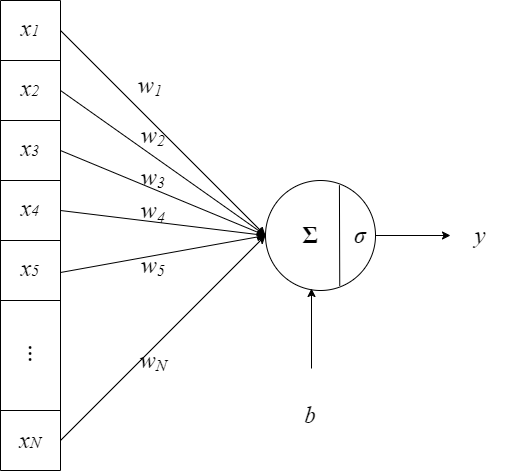
\includegraphics[width=0.5\linewidth]{figures/neuron.drawio.png}
    \caption{神經元示意圖}
    \label{fig:single-neuron}
\end{figure}

        結合數個神經元的運算,羅氏(Rosenblatt)於 1958 年 \cite{rosenblatt_perceptron_1958} 提出感知器(Perceptron)模型。根據通用近似定理(Universal Approximation Theorem)\cite{funahashi_approximate_1989} ,感知器理論上可逼近任意函數。然而,後續研究發現單層的感知器具有如「線性不可分」\footnote{例如無法貼合異或(Exclusive OR,XOR)運算等函數} 等先天限制,使其曾經一度不被看好。

        為了突破該缺陷,人們嘗試在輸入與輸出層之間增加「隱藏層(Hidden Layer)」,成為「多層感知器(Multilayer Perceptron,MLP)」,如圖 \ref{fig:mlp} 所示。藉助隱藏層的幫助,多層感知器可對輸入進行多次非線性轉換,大大拓展了模型的適用範圍。此模型是透過「加深隱藏層」得來,現今為人們熟知的「深層類神經網路(Deep Neural Network)」即由此得名。

\begin{figure}
    \centering
    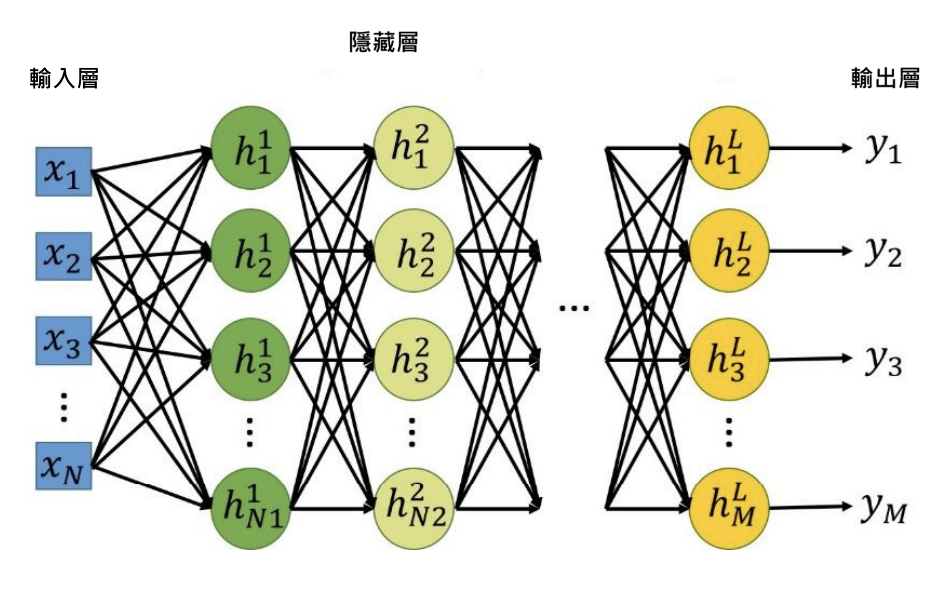
\includegraphics[width=0.8\linewidth]{figures/nnout.png}
    \caption{多層感知器/深層類神經網路示意圖}
    \label{fig:mlp}
\end{figure}

        % 確認那個「大量」跟「應用」有沒有掉字
        藉助深層類神經網路的彈性,我們可以透過大量訓練資料來訓練模型,藉此逼近應用任務中欲近似的函數 $f$,該函數蘊藏在資料集 $\mathcal{D} = \{(x_i, y_i)\}_{i=1}^N$ 中,其中每個資料點 $(x_i, y_i)$ 為輸入與輸出間的配對,即對於 $N$ 個資料點都有 
\begin{align}
    y_i = f(x_i) \ \  \forall i \in \{1, \cdots\cdots, N\}
\end{align}
之關係。為了使這個函數更加逼近目標函數 $f$,類神經網路會構建一個逼近中的函數 $f_{\theta_t}(\cdot)$ 。透過不停的迭代,模型對資料集 $\mathcal{D}$ 的每一筆資料 $x$ 給出預測 $f_{\theta_t}(x)$ 。透過某個減損函數(Loss Function)$\mathcal{L}$ 計算出誤差(Error),此誤差對參數 $\theta_t$ 求出梯度(Gradient)後將指示模型更新的方向,以此乘上學習率(Learning Rate)$\eta$ 後從參數  $\theta_t$ 減去,便能對整個模型進行更新,使之更有機會接近目標函數 $f$。由於此過程是依照梯度使得函數 $\mathcal{L}$ 逐步降低,以此獲名「梯度下降法(Gradient Descent)」,其公式如下:
\begin{align}
    \theta_{t+1} \leftarrow \theta_{t} - \eta \nabla_\theta\mathcal{L}(\mathcal{D}, f_{\theta_t}(\cdot))
\end{align}
其中,$t$ 為當前的迭代數,$\theta_t$ 為當前模型參數,$\theta_{t+1}$ 為更新後的模型參數。

        在此模型更新的過程中,減損函數承擔著指引模型逼近的角色,因此根據應用的任務不同,常見的減損函數包括
\begin{itemize}
    \item 均方誤差(Mean Squared Error,MSE):一般用於迴歸(Regression)問題,直接計算兩數值之間的差距的平方和
          \begin{align}
              \mathcal{L}_{\text{MSE}}(y_i, \hat{y}_i) = \frac{1}{N} \sum_{i=1}^{N} (y_i - \hat{y}_i)^2
          \end{align}
          \textcolor{red}{\(\hat{y}_i\) 是……??????????}
    \item 交叉熵(Cross-entropy,CE):一般用於分類(Classification)問題,著重計算兩個機率分佈之間的差異
          \begin{align}
              \mathcal{L}_{\text{CE}}(y_i, \hat{y}_i) = - \sum_{i=1}^{N} \left[ y_i \log(\hat{y}_i) + (1 - y_i) \log(1 - \hat{y}_i) \right]
          \end{align}
\end{itemize}

        透過上述的訓練方式可以得知,類神經網路的訓練需要相當龐大且複雜的運算過程,因此剛提出時仍舊難以應用於現實應用中。

        為了提高函數貼合的效率,魯氏(Rumelhart)與辛氏(Hinton)等人 \cite{rumelhart_learning_1986, rumelhart_learning_1987} 提出了反向傳播(Backpropagation)演算法,旨在將上述的更新過程,藉助鏈鎖率(Chain Rule)的幫助,由隱藏層逐層反向傳播至輸入層,對整個類神經網路進行修正。

        反向傳播演算法的設計,正好能配合圖形處理器(Graphics Processing Unit,GPU)等硬體裝置的優勢,以平行運算能力加速函數貼合(Fit)的效率。由此開始,這種透過深層類神經網路,從大量資料集中發掘函數關係的機器學習演算法,被稱為深層學習(Deep Learning)。 類神經網路在各個領域的泛化能力(Generalizability)已經得到前所未有的效能,包含電腦視覺、語音處理和自然語言處理,因此深層學習在近年成為人工智慧發展的主流。

        然而,根據資料特性的不同,並不是所有的資料都適用簡單的「輸入與輸出配對」的模式。研究者根據任務需求,發展出了不同架構的類神經網路以適應資料特性。前述最基本的深層類神經網路,由於資料是直接由輸入層,通過逐層的矩陣運算得到輸出,因此被稱之為「前饋式類神經網路(Feed Forward Network,FFN)」。

        藉由調整各神經元之間的連接關係,發展出卷積式(Convolutional)、遞迴式(Recurrent)與轉換器(Transformer)類神經網路等架構變體,以適應如影像、語音和文字等不同型態的資料。這些架構在語音與文字處理被普遍使用,接下來將逐一分別介紹:

\subsection{卷積式類神經網路}

  卷積式類神經網路(Convolutional Neural Network,CNN)為 1998 年由楊氏(LeCun) \cite{lecun_gradient-based_1998} 提出,旨在以訊號處理的卷積(Convolution)運算,模擬生物的視覺皮質感知 \cite{hubel_receptive_1959} 。

\begin{figure}
    \centering
    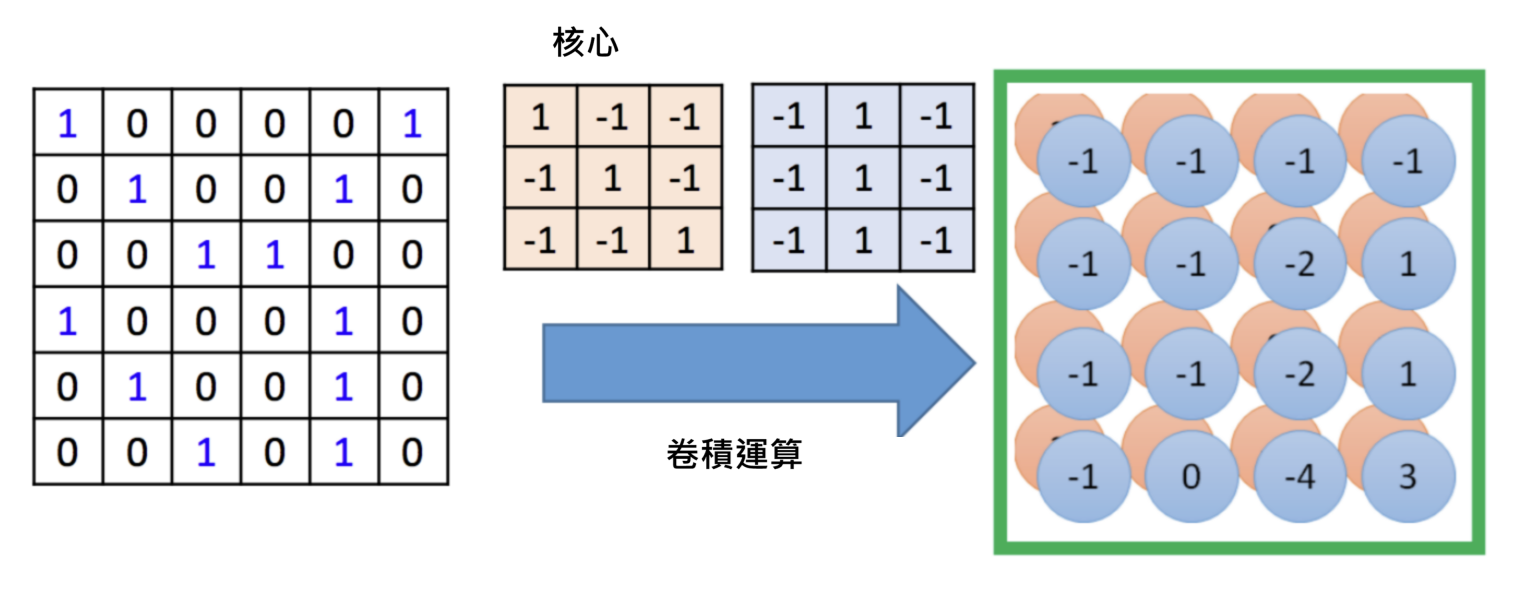
\includegraphics[width=0.9\linewidth]{figures/cnnnew.png}
    \caption{卷積式類神經網路示意圖,取自李宏毅教授的課程投影片}
    \label{fig:cnn}
\end{figure}

        如圖 \ref{fig:cnn} 所示,卷積式類神經網路透過核心(Kernel),對輸入的資料 --- 如圖中的二維矩陣 --- 進行卷積運算,獲得該輸入的特徵圖(Feature Map)。核心帶來的移動不變性(Shift-invariance)非常適用於捕捉二維影像中的局部特徵,以作為類神經網路分辨資料的依據。

        有別於影像處理中,資料多以二維矩陣表示像素 (Pixel)三原色的亮度數值,因此以二維的卷積運算為主;由於語音時常處理時間軸之上的訊號,包含聲波波形(Waveform)、時頻譜(Spectrogram)或聲學特徵,因此一維的卷積式模型也時常出現,以模仿人耳聽覺對時變訊號的窗框(Window)的效應,進而觀察到語音中在不同解析度(Resolution)的資訊。

\subsection{遞迴式類神經網路與序列至序列模型}

\subsubsection{遞迴式類神經網路}

  遞迴式類神經網路(Recurrent Neural Network,RNN)常用於處理隨時間變化的序列資料,特別是語音與文字等等,順序資訊相當關鍵的各種語言任務。

        為了處理需要記憶和狀態的資料類型,遞迴式類神經網路的輸出會重新接回輸入層,使得前一個時間點(Timestep)的資料與內部狀態會繼續影響後續的時間點。

        常用的遞迴式類神經網路類型有長短期記憶(Long Short-term Memory,LSTM)\cite{hochreiter1997long} 和閘門循環單元(Gated Recurrent Unit,GRU)\cite{cho-etal-2014-properties} 等。

        遞迴式類神經網路通常用在處理序列至序列的應用,例如語音辨識、語音合成或機器翻譯等和語言密切相關的任務中。

\subsubsection{序列至序列模型}

  由於許多語言資料通常以兩個序列互相配對的形式呈現,因此專門處理這類資料的模型被稱為序列至序列模型(Sequence-to-sequence,Seq2seq)\cite{sutskever2014sequence}。此類模型的典型架構由編碼器(Encoder)和解碼器(Decoder)組成,旨在模擬輸入與輸出序列之間的變化與相依關係(Dependency)。

        序列到序列模型一般有兩種模式:其一是每個時間點都生成一個輸出的向量,適用於輸入與輸出序列等長的任務,這種模式被稱為符記分類(Token Classification);但更常見的情況是,輸入與輸出序列的長度並不相同。處理後者的典型作法是讓編碼器將輸入序列依據時間,一步一步輸入編碼器,將序列編碼為內部表徵(Latent Representation)。完成編碼後,編碼器將最後一個時間點的表徵用以代表整個序列,稱為「語境向量(Context Vector)」。該向量接著被傳遞給解碼器,依序生成輸出序列。

\subsection{專注機制與轉換器類神經網路}

\subsubsection{專注機制}

  由於遞迴式類神經網路需要處理整個序列的編碼和解碼資訊,對時間點距離較遠的輸入容易被遺忘,亦即難以處理長期相依性(Long-term Dependency)問題。為了解決這種困境,巴氏(Bahdanau)等人提出了「專注機制(Attention Mechanism)」\cite{bahdanau2014neural}。該機制讓解碼器將輸入序列的每個訊號都視作「部分的」語境向量,由對不同時間點的向量加權合計獲得,使得在生成輸出序列時能依據當時的需求從輸入序列中提取所需的訊息。專注機制的引入,使得序列至序列模型在處理如語音辨識、機器翻譯等任務時效能大大改善。

\subsubsection{轉換器類神經網路}

  儘管遞迴式類神經網路善於處理時序資料,但其難以平行化的架構限制了其在訓練和推理(Inference)時的效率。2017 年,瓦氏(Vaswani)等人 \cite{vaswani2017attention} 提出了完全由專注機制構成、不依賴遞迴運算的序列至序列模型,並稱之為「轉換器(Transformer)」,以解決機器翻譯等任務。

        轉換器類神經網路一般包含編碼器和解碼器兩部分,均為多層架構。圖 \ref{fig:tfm_arch} 展示完整的轉換器架構圖,以下分別介紹其主要元件:

\paragraph{位置編碼(Positional Encoding)}

  對於編碼器或解碼器的輸入序列,模型先對序列中不同位置的時間點進行編碼,取代遞迴式類神經網路逐步運算的過程,使其能在平行計算的同時考慮不同時間點的影響。編碼的函數可依照需求變換,如原始的轉換器採用三角函數進行位置編碼,而在語音模型中,有時也會採用卷積式網路以捕捉輸入的細微資訊。

        經過位置編碼後,向量會通過每一個轉換器層(Transformer Layer),進行以多頭專注(Multi-head Attention)為主的一連串運算:

\paragraph{多頭專注}

  轉換器層中的專注機制涉及三個輸入向量:詢向量(Query)$Q$、鑰向量(Key)$K$ 和值向量(Value)$V$。專注機制運算如下:
\begin{align}
    \text{Attention}(Q, K, V) = \text{softmax}
    \left(
    \frac{QK^\top}{\sqrt{d_k}}
    \right)
    V
\end{align}
其中 $\text{softmax}$ 為正規化指數函數,$d_k$ 為鑰向量 $K$ 的維度。這一運算首先通過鑰向量和詢向量的內積計算專注權重,而後為避免受維度過大影響而縮小為 $\sqrt{d_k}$ 分之一,最後通過正規化指數函數使得權重總和為 1 ,以此分配給值向量進行加權。

        為應對多樣的輸入訊號,每個轉換器層具備多個獨立的專注機制,對三組輸入向量先進行各自不同的 $W^Q$、$W^K$、$W^V$ 線性轉換,稱為「多頭專注(Multi-head Attention)」。對於第 $i$ 個專注頭(Head)有
\begin{align}
    \text{head}_i = \text{Attention}(QW^Q_i,KW^K_i,VW^V_i)
\end{align}
          \textcolor{red}{\(\text{Attention}(\cdot, \cdot, \cdot)\) 是……??????????} \\
最後,若有 $h$ 個專注頭,多頭專注模組會將多個頭的結果進行串接(Concatenate),經過線性轉換 $W^O$ 作為模組輸出
\begin{align}
    \text{MultiHead}(Q, K, V) = \text{Concat}(\text{head}_1, \cdots\cdots, \text{head}_h) W^O
\end{align}

\paragraph{其他層內運算}

  每層轉換器層在經過多頭專注運算後,會依序進行以下三個步驟:

\begin{enumerate}
    \item 與輸入向量透過殘差連接(Residual Connection)相加,隨後進行層正規化(Layer Normalization)以穩定訓練。
    \item 將此結果通過一個簡單的前饋式類神經網路對向量做線性轉換。
    \item 再將前饋網路的輸入與輸出再次計算殘差總和後,進行層正規化輸出。
\end{enumerate}

        以上為轉換器被提出時的最原始模型,其後對殘差連接、層正規化的安排也存在各類變體。

\paragraph{跨專注機制(Cross-atttention)}

  由於解碼器需要來自編碼器的輸入序列資訊幫助輸出,因此,原本在編碼器層中的自專注機制,在解碼器中會再經過一次跨專注機制的運算,使用編碼器提供的詢向量和鑰向量對解碼器的值向量進行專注運算。

\begin{figure}
    \centering
    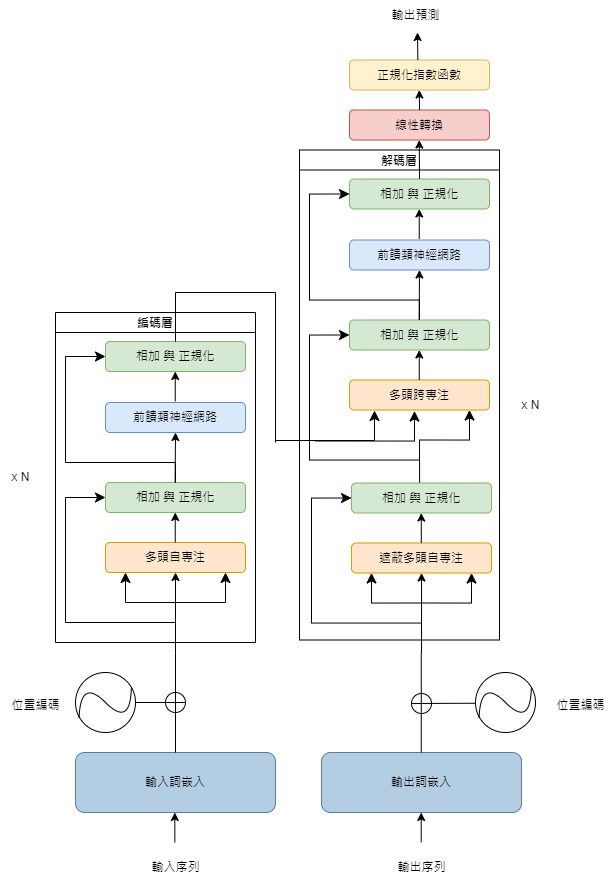
\includegraphics[width=0.9\linewidth]{figures/tfm_arch.drawio.png}
    \caption{轉換器架構圖}
    \label{fig:tfm_arch}
\end{figure}

        由於轉換器不需要對每個時間點逐一運算,使其得以實現高度平行化,類神經網路得以透過專注機制同時進行序列資料的大量訓練。這種可擴展性(Scalability)使其在自然語言和語音處理上取得了巨大的進展,幾乎取代了原先遞迴式類神經網路的應用場景,近年來甚至被應用在圖像類的資料上\cite{dosovitskiy2021image},展現了此種模型架構的彈性與泛用性,成為目前最前沿的人工智慧主流架構。

        除了模型架構,機器學習中不可或缺的另一大部分是對資料的編碼過程。如何更有效率的讓機器理解、處理和輸出資料,是機器學習乃至深層學習的一大課題。面對捉摸不定、抽象且變化萬千的人類語言,語音和文字處理中的表徵學習尤為重要。

\section{表徵與自監督式學習}

\subsection{特徵抽取與表徵學習}

  不論採用何種模型,為了讓機器可以處理並捕捉輸入資料中的訊號與模式(Pattern),包括如何對資料編碼和運算的步驟,在機器學習中稱之為特徵抽取(Feature Extraction)或表徵學習(Representation Learning),這是模型建構中不可或缺的重要步驟。

        對於抽象的語言概念,早期工程領域根據對語音和文字的理解,分別進行了不同的處理。對於離散且可計數的文字,人們使用詞頻統計衍生出如 n 連詞(n-gram)、TF-IDF(Term-Frequency Inverse Document Frequency)等特徵作為模型學習的前處理步驟;而對於連續且複雜的語音,工程師則透過聲學原理與訊號處理的知識,使用如濾波器組(Filter Bank)、梅爾倒頻譜係數(Mel-Frequency Cepstrum Coefficient,MFCC)等特徵,類比人耳捕捉語音訊號的過程。

        在深層學習逐漸發展的過程中,自然語言處理領域的一大里程碑是米氏(Mikolov)提出的「word2vec」模型 \cite{mikolov_efficient_2013},該模型以連續的向量表徵(Vector Representation)取代稀疏(Sparse)的統計數據,對離散的文字單詞進行「詞嵌入(Word Embedding)」編碼。通過大量文本運算,將各單詞之間的共現(Collocation)以跳躍詞(Skip-gram)、連續詞袋(Continuous Bag-of-Word,CBOW)等演算法轉換成高維向量空間中的點,找出每個單詞最適合的語義表徵。爾後,為了更細緻地捕捉同一單詞在不同句子中的脈絡變化,ELMo(Embeddings from Language Model)\cite{peters_deep_2018} 提出了「含上下文詞嵌入(Contextualized Embedding)」的概念,使得各單詞在運算表徵的過程中可以根據上下文進行些微調整。

\subsection{自監督學習}

  隨著轉換器模型的提出,BERT(來自轉換器的雙向編碼器表徵,Bidirectional Encoder Representations from Transformers)\cite{devlin_bert_2019} 被提出。通過自專注機制,工程師們無需依賴人工標記,透過預先設定任務(Pretext Task)引導模型從大量文本中自行找出更細緻且考量前後文(Contextualized)的語義關係,並在許多文字任務上獲得了優異的成績。

        自此,楊氏(LeCun)將這種以特定任務作為引導、藉助資料本身的結構替代標註,從大量未標註資料中進行學習資料模式(Pattern)的訓練方式,稱之為「自監督學習(Self-supervised Learning,SSL)」。BERT 的成功使自監督學習得以大行其道,並出現了許多由巨量資料進行預訓練(Pre-train)的基石模型(Foundation Model),有效解決了語言處理領域中的標註資料稀缺的問題。人們在解決語言相關任務時,不需從頭蒐集資料與進行耗時耗能的訓練過程,而是可以利用基石模型優良的泛化(Generalization)能力,解決各種應用任務的需求。相比於預訓練的任務,這些更貼近日常現實的任務被稱為「下游任務(Downstream Task)」,能應對廣泛的下游任務種類,這是基石模型最大的優勢。

        有鑑於文字處理方面的成功,語音領域的研究者嘗試將相似模式應用於語音,眾多語音基石模型隨之出現。大量的語音資料庫幫助模型萃取出有助於下游任務的語音表徵(Speech Representation),在各種任務上獲得了優於傳統聲學特徵的表現。語音表徵具備的無窮潛力,逐漸成為聲學特徵之外的新選擇。

        依照這些語音自監督模型的預訓練學習模式,可大致分為重建式、預測式與對比式模型。以下分別介紹這三類模式:

\subsubsection{重建式學習(Reconstruction Learning)}

  此類模型通過對輸入訊號進行擾動(Perturb)後,期望模型將被更動的輸入重新預測回原始資料,通常減損函數表示為:
\begin{align}
    \mathcal{L}_{recon} = \mathbb{E}_x[|f_\theta(\tilde{x}) - x|]
\end{align}
其中 $\tilde{x}$ 為擾動後的資料,$f_\theta(\cdot)$ 為模型函數。擾動方式通常以遮蔽為主,在文字處理中以 BERT 為代表,稱為「遮蔽語言模型(Masked Language Model,MLM)」。在語音中,採用此方式學習的有 Mockingjay \cite{liu_mockingjay_2019}、TERA \cite{t_tera_2021} 等模型。  % NPC

\subsubsection{預測式學習(Predictive Learning)}

  此類模型通過預訂一些學習目標函數,製造類似輸入與輸出的配對資料,讓模型預測該函數的結果來學習資料中的特定結構。其訓練減損函數可表示為:
\begin{align}
    \mathcal{L}_{pred} = \mathbb{E}_x[\text{eval}(f_\theta(x), \hat{f}(x))]
\end{align}
其中 $\hat{f}$ 是期望模型學習的目標函數,$f_\theta(\cdot)$ 為模型函數,$\text{eval}$ 是用來評估預測好壞的標準。

        目標函數的典型代表是自迴歸(Autoregressive),期望模型預測未來時間點的輸入表徵。文字方面以生成式預訓練轉換器(Generative Pretrained Transformer,GPT)系列 \cite{radford_language_nodate, brown_language_2020}為代表,語音上的自迴歸預測編碼(Autoregressive Predictive Coding,APC) \cite{chung_generative_2020} 也是採用此種模式。此外,語音基石模型還可以使用其他訓練目標,如 PASE+ \cite{ravanelli_multi-task_2020} 預測其他模型的表徵,而本文著重探究的「隱藏單元 BERT(Hidden-unit BERT,HuBERT)」\cite{hsu_hubert_2021, hsu_hubert_2021-2} 則以預測分群(Cluster)後的輸入表徵為目標,這些預測目標又被視為虛擬標註(Pseudo-label),後文將著重探討。

\subsubsection{對比式學習(Contrastive Learning)}

  此學習方式的訓練目標是要求模型區分正樣本(Positive Sample)與負樣本(Negative Sample)的差異,減損函數通常定義為:
\begin{align}
    \mathcal{L}_{contr} = -\mathbb{E}_x\left[\log
        \left(
        {\frac
            {\sum_{\tilde{x} \in x_{pos}}\exp(\text{sim}(x, \tilde{x}))}
            {\sum_{\tilde{x} \in \mathcal{X}}\exp(\text{sim}(x, \tilde{x}))}
        }\right)\right]
\end{align}

        其中 $x$ 為輸入,$x_{pos}$ 為正樣本,$\mathcal{X}$ 為包含正負樣本的資料集,$\text{sim}(\cdot, \cdot)$ 是評估兩個樣本相似程度的函數,常用的相似度函數為內積運算得出的餘弦相似度(Cosine Similarity)。語音上最早使用對比式學習的模型為對比預測編碼(Contrastive Predictive Coding,CPC)\cite{maekaku2022speech},之後如 Wav2vec \cite{schneider2019wav2vec}、Modified CPC \cite{rivière2020unsupervised}、Wav2vec 2.0 \cite{baevski2020wav2vec} 等模型亦是以對比正負樣本的模式訓練,但訓練時正負樣本的定義有所差異,如 Wav2vec 僅以時間維度上相同的向量為正樣本,其餘則將固定時間內的向量皆視為正樣本。

        對比式學習通過正負樣本的定義,將預訓練任務形塑為分類問題,因此減損函數本質上為交叉熵,使模型能夠判斷訓練資料中的結構差異。

\subsection{向量量化與離散單元}

  語音訊號雖然記錄語言資訊,卻與影像資料一樣都是連續數值資料,不像離散的文字較易處理,因此發展出了許多應用廣泛的模型。為了使語音模型訓練可以套用自然語言處理領域的演算法,從連續語音中找出離散表徵逐漸成為研究趨勢,這類研究被稱為「聲學單元發掘(Acoustic Unit Discovery,AUD)」。

        由於語言概念本質上是離散符號,向量量化技術常用於涉及語言標註的情境,如電腦視覺經典的量化向量變分自編碼器(Vector-Quantized Variational Autoencoder,VQ-VAE)\cite{van2017neural},利用影像標註的離散語言單詞特性,使模型學習的表徵向量被約束在編碼簿(Codebook) 的幾個向量中。

        在語音領域,基於 Wav2vec 之上的 Vq-wav2vec \cite{baevski2019vq} 和 Wav2vec 2.0 將連續的語音特徵量化加入訓練目標中,在語音辨識等任務上取得了顯著進步。

        HuBERT \cite{hsu_hubert_2021-2} 則先對連續的 MFCC 特徵進行 K-平均(K-Means)演算法分群,以所得的群心(Centroid)或碼字(Code Word)編號作為訓練目標,實施類似 BERT 的遮蔽語言模型訓練,並改以此次訓練得到的語音表徵為目標,再次分群後實施第二次訓練。這些經過兩輪訓練後,從模型表徵分群得到的群心,被視為「隱藏單元(Hidden Unit)」,呈現了語音訊號中的代表性聲學特徵。透過找出隱藏單元的過程,HuBERT 在低資源情況下達到與 Wav2vec 2.0 相近的語音辨識成績。

\subsection{無文字(Textless)架構}

  奠基於 HuBERT 等語音基石模型的成功,利用隱藏單元的概念,將大量語音資料表徵進行 K-平均演算法,作為這些語音訊號的虛擬標註。如此得到的大量離散隱藏單元形成了「虛擬文字(Pseudo-text)」的語料庫,基於這些離散單元訓練的語言模型,稱為「生成式口語語言模型(Generative Spoken Language Model,GSLM)」\cite{lakhotia_generative_2021-1}。配合反向語音合成訓練基於離散單元的語音生成模型,整體架構完全不依賴文字標註,訓練出純語音語言模型,稱為「無文字(Textless)架構」\cite{noauthor_textless_2021}。

        無文字模式在語音問答(Spoken Question Answering)\cite{lin2022dual}和語音到語音翻譯 (Speech-to-speech Translation)\cite{chen_speech--speech_2023}中取得了前所未有的進展。這些「離散單元(Discrete Unit)」被視為類似文字卻不依賴人類文字標記的語音表徵,具有儲存位元率低和可套用文字語言模型訓練模式的優勢,受到語音社群的廣泛借鑑,後續也帶出了許多如\cite{zhang2024speechtokenizer} 等將語音以離散表徵編碼的研究。

        雖然在系統與應用任務上取得了成功,但這些離散單元本身與文字的差異,及其對語音語言模型訓練的幫助,仍是領域內探討的焦點。有鑑於此,本論文基於語言知識,從最接近文字且與語音訊號最相關的「音位(Phoneme)」開始探討,期望了解離散單元能帶來的特徵及其對後續應用的幫助。

\section{本章節總結}

  本章節首先介紹了深層學習模型的核心部件 --- 類神經網路的基本原理,隨後對本論文研究的核心 --- 「語音表徵」與「離散單元」的發展與歷史進行了梳理。接下來的章節將緊扣這些基石模型得到的離散特徵,對其與「音位」這類語音學標記之間的統計關係進行更深入分析。


\chapter{背景知識}

\section{深層類神經網路}

\subsection{簡介}

  深層類神經網路(Deep Neural Network,DNN)是由神經科學家麥氏(McCulloch)與皮氏(Pitts)於 1943 年提出 \cite{mcculloch_logical_1943} 的計算模型,靈感取自連結主義(Connectionism)的核心主張 --- 以模仿生物神經網路的連結方式模擬複雜的心智活動。

        為模擬神經細胞處理訊號的過程,深層類神經網路最基本的單位稱為「神經元(Neuron)」,其本質為線性分類器。每個神經元接收的輸入數值 $x = (x_1, x_2, \cdots\cdots, x_N)$ 是一個 $N$ 維向量,每一維會被賦予一個權重(Weight) $w = (w_1, w_2, \cdots\cdots, w_N)$  ,加權後總和再加上偏差值(Bias) $b$,得到線性輸出值。為了模擬神經細胞的觸發過程,該分類器常被加上非線性的激發函數(Activation Function)$\sigma$ 的轉換,才得到最終輸出值 $y$。如圖 \ref{fig:single-neuron}所示,神經元的運算規則以下列數學式描述:
\begin{align}
    y = \sigma(w^T x + b)
\end{align}
常見的激發函數包含線性整流單元(Rectified Linear Unit,ReLU)、S 函數(Sigmoid Function)或雙曲正切函數(Hyperbolic Tangent Function,$\tanh$)等等。

\begin{figure}
    \centering
    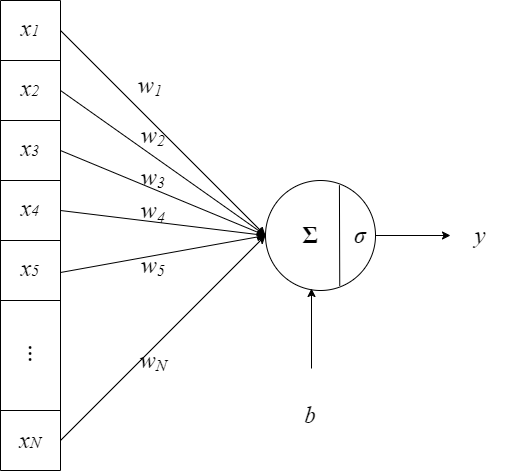
\includegraphics[width=0.5\linewidth]{figures/neuron.drawio.png}
    \caption{神經元示意圖}
    \label{fig:single-neuron}
\end{figure}

        結合數個神經元的運算,羅氏(Rosenblatt)\cite{rosenblatt_perceptron_1958} 於 1958 年提出感知器(Perceptron)模型。根據通用近似定理(Universal Approximation Theorem)\cite{funahashi_approximate_1989} ,感知器理論上可逼近任意函數。然而,後續研究發現單層的感知器具有如「線性不可分」\footnote{例如無法貼合異或(Exclusive OR,XOR)運算等函數} 等先天限制,使其曾經一度不被看好。

        為了突破該缺陷,人們嘗試在輸入與輸出層之間增加「隱藏層(Hidden Layer)」,成為「多層感知器(Multilayer Perceptron,MLP)」,如圖 \ref{fig:mlp} 所示。藉助隱藏層的幫助,多層感知器可對輸入進行多次非線性轉換,大大拓展了模型的適用範圍。此模型是透過「加深隱藏層」得來,現今為人們熟知的「深層類神經網路」即由此得名。

\begin{figure}
    \centering
    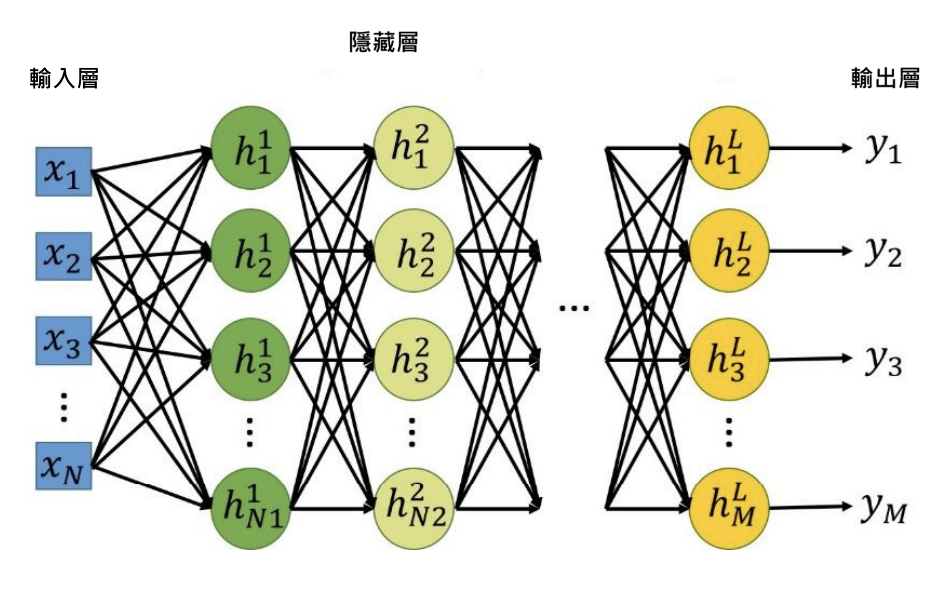
\includegraphics[width=0.8\linewidth]{figures/nnout.png}
    \caption{多層感知器/深層類神經網路示意圖}
    \label{fig:mlp}
\end{figure}
        % 確認那個「大量」跟「應用」有沒有掉字
        藉助深層類神經網路的彈性,我們可以透過大量訓練資料來訓練模型,藉此逼近應用任務中欲近似的函數 $f$,該函數蘊藏在資料集 $\mathcal{D} = \{(x_i, y_i)\}_{i=1}^N$ 中,其中每個資料點 $(x_i, y_i)$ 為輸入與輸出間的配對,即對於 $N$ 個資料點都有 
\begin{align}
    y_i = f(x_i) \ \  \forall i \in \{1, \cdots\cdots, N\}
\end{align}
之關係。為了使這個函數更加逼近目標函數 $f$,類神經網路會構建一個逼近中的函數 $f_{\theta_t}(\cdot)$ 。透過不停的迭代,模型對資料集 $\mathcal{D}$ 的每一筆資料 $x$ 給出預測 $f_{\theta_t}(x)$ 。透過某個減損函數(Loss Function)$\mathcal{L}$ 計算出誤差(Error),此誤差對參數 $\theta_t$ 求出梯度(Gradient)後將指示模型更新的方向,以此乘上學習率(Learning Rate)$\eta$ 後從參數  $\theta_t$ 減去,便能對整個模型進行更新,使之更有機會接近目標函數 $f$。由於此過程是依照梯度使得函數 $\mathcal{L}$ 逐步降低,以此獲名「梯度下降法(Gradient Descent)」,其公式如下:
\begin{align}
    \theta_{t+1} \leftarrow \theta_{t} - \eta \nabla_\theta\mathcal{L}(\mathcal{D}, f_{\theta_t}(\cdot))
\end{align}
其中,$t$ 為當前的迭代數,$\theta_t$ 為當前模型參數,$\theta_{t+1}$ 為更新後的模型參數。

        在此模型更新的過程中,減損函數承擔著指引模型逼近的角色,因此根據應用的任務不同,常見的減損函數包括
\begin{itemize}
    \item 均方誤差(Mean Squared Error,MSE):一般用於迴歸(Regression)問題,直接計算兩數值之間的差距的平方和
          \begin{align}
              \mathcal{L}_{\text{MSE}}(y_i, \hat{y}_i) = \frac{1}{N} \sum_{i=1}^{N} (y_i - \hat{y}_i)^2
              \label{eq:mse}
          \end{align}
          % \textcolor{red}{\(\hat{y}_i\) 是……??????????}

          式 \eqref{eq:mse} 中的 \(\hat{y}_i\) 是模型預測的輸出值,理想上希望愈接近資料標註 \(y_i\) 愈好。
    \item 交叉熵(Cross-entropy,CE):一般用於分類(Classification)問題,著重計算兩個機率分佈之間的差異
          \begin{align}
              \mathcal{L}_{\text{CE}}(y_i, \hat{y}_i) = - \sum_{i=1}^{N} \left[ y_i \log(\hat{y}_i) + (1 - y_i) \log(1 - \hat{y}_i) \right]
          \end{align}
          式中的 \(\hat{y}_i\) 與 \(y_i\) 所代表的意義和式 \eqref{eq:mse} 相同,分別表示模型預測值與資料標註,只是計算兩者差距的方式有異。
\end{itemize}

        透過上述的訓練方式可以得知,類神經網路的訓練需要相當龐大且複雜的運算過程,因此剛提出時仍舊難以應用於現實應用中。

        為了提高函數貼合的效率,魯氏(Rumelhart) \cite{rumelhart_learning_1986} 與辛氏(Hinton) \cite{rumelhart_learning_1987} 等人提出了反向傳播(Back-Propagation)演算法,旨在將上述的更新過程,藉助鏈鎖率(Chain Rule)的幫助,由隱藏層逐層反向傳播至輸入層,對整個類神經網路進行修正。

        反向傳播演算法的設計,正好能配合圖形處理器(Graphics Processing Unit,GPU)等硬體裝置的優勢,以平行運算能力加速函數貼合(Fit)的效率。由此開始,這種透過深層類神經網路,從大量資料集中發掘函數關係的機器學習演算法,被稱為「深層學習(Deep Learning)」。 類神經網路在各個領域的泛化能力(Generalizability)已經得到前所未有的效能,包含電腦視覺、語音處理和自然語言處理,因此深層學習在近年成為人工智慧發展的主流。

        然而,根據資料特性的不同,並不是所有的資料都適用簡單的「輸入與輸出配對」的模式。研究者根據任務需求,發展出了不同架構的類神經網路以適應資料特性。前述最基本的深層類神經網路,由於資料是直接由輸入層,通過逐層的矩陣運算得到輸出,因此被稱之為「前饋式類神經網路(Feed-Forward Network,FFN)」。

        藉由調整各神經元之間的連接關係,發展出卷積式(Convolutional)、遞迴式(Recurrent)與轉換器(Transformer)類神經網路等架構變體,以適應如影像、語音和文字等不同型態的資料。這些架構在語音與文字處理被普遍使用,接下來將逐一分別介紹:

\subsection{卷積式類神經網路}

  卷積式類神經網路(Convolutional Neural Network,CNN)為 1998 年由楊氏(LeCun) \cite{lecun_gradient-based_1998} 提出,旨在以訊號處理的卷積(Convolution)運算,模擬生物的視覺皮質感知 \cite{hubel_receptive_1959} 。

\begin{figure}
    \centering
    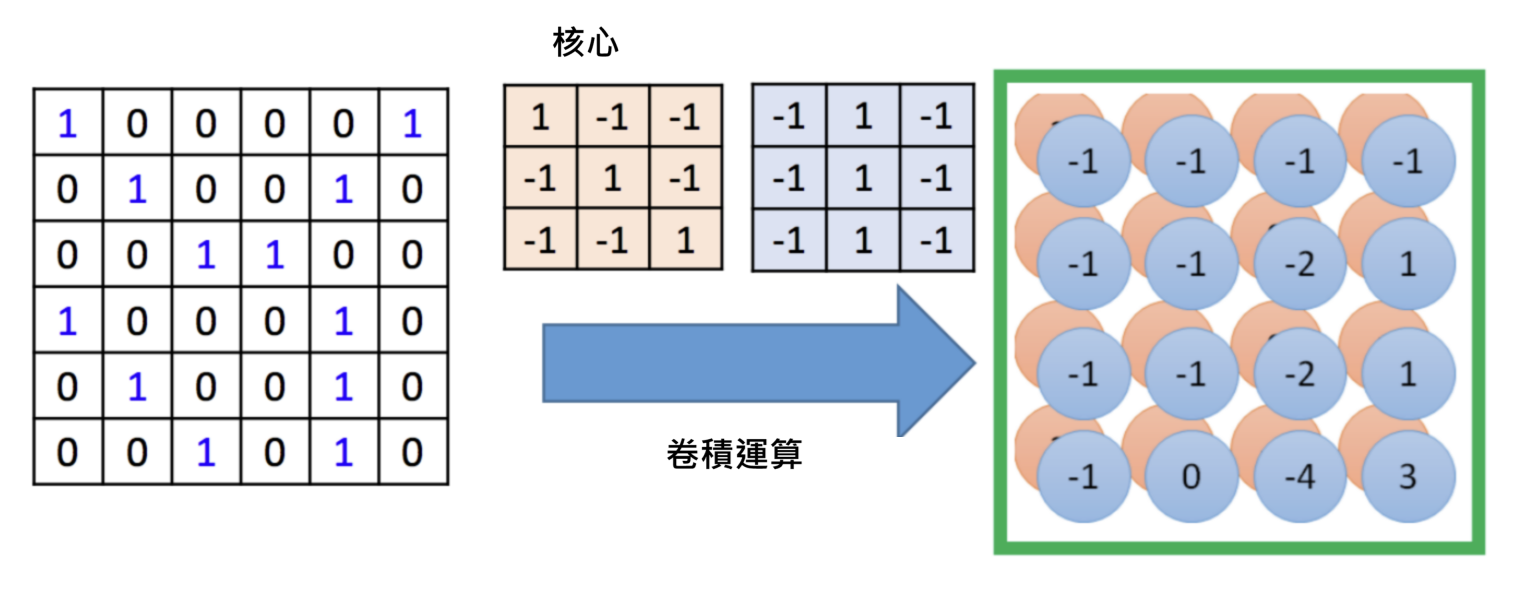
\includegraphics[width=0.9\linewidth]{figures/cnnnew.png}
    \caption{卷積式類神經網路示意圖,取自李宏毅教授的課程投影片}
    \label{fig:cnn}
\end{figure}

        如圖 \ref{fig:cnn} 所示,卷積式類神經網路透過核心(Kernel),對輸入的資料 --- 如圖中的二維矩陣 --- 進行卷積運算,獲得該輸入的特徵圖(Feature Map)。核心帶來的移動不變性(Shift-invariance)非常適用於捕捉二維影像中的局部特徵,以作為類神經網路分辨資料的依據。

        有別於影像處理中,資料多以二維矩陣表示像素 (Pixel)三原色的亮度數值,因此以二維的卷積運算為主;由於語音時常處理時間軸之上的訊號,包含聲波波形(Waveform)、時頻譜(Spectrogram)或聲學特徵,因此一維的卷積式模型也時常出現,以模仿人耳聽覺對時變訊號的窗框(Window)的效應,進而觀察到語音中在不同解析度(Resolution)的資訊。

\subsection{遞迴式類神經網路與序列至序列模型}

\subsubsection{遞迴式類神經網路}

  遞迴式類神經網路(Recurrent Neural Network,RNN)常用於處理隨時間變化的序列資料,特別是語音與文字等等,順序資訊相當關鍵的各種語言任務。為了處理需要記憶和狀態的資料類型,遞迴式類神經網路的輸出會重新接回輸入層,使得前一個時間點(Timestep)的資料與內部狀態會繼續影響後續的時間點。常用的遞迴式類神經網路類型有長短期記憶(Long Short-term Memory,LSTM)\cite{hochreiter1997long} 和閘門循環單元(Gated Recurrent Unit,GRU)\cite{cho-etal-2014-properties} 等。

        遞迴式類神經網路通常用在處理序列至序列的應用,例如語音辨識、語音合成或機器翻譯等和語言密切相關的任務中。

\subsubsection{序列至序列模型}

  由於許多語言資料通常以兩個序列互相配對的形式呈現,因此專門處理這類資料的模型被稱為「序列至序列模型(Sequence-to-sequence,Seq2seq)」\cite{sutskever2014sequence}。此類模型的典型架構由編碼器(Encoder)和解碼器(Decoder)組成,旨在模擬輸入與輸出序列之間的變化與相依關係(Dependency)。

        序列到序列模型一般有兩種模式:其一是每個時間點都生成一個輸出的向量,適用於輸入與輸出序列等長的任務,這種模式被稱為「符記分類(Token Classification)」;但更常見的情況是,輸入與輸出序列的長度並不相同。處理後者的典型作法是讓編碼器將輸入序列依據時間,一步一步輸入編碼器,將序列編碼為內部表徵(Latent Representation)。完成編碼後,編碼器將最後一個時間點的表徵用以代表整個序列,稱為「語境向量(Context Vector)」。該向量接著被傳遞給解碼器,依序生成輸出序列。

\subsection{專注機制與轉換器類神經網路}

\subsubsection{專注機制(Attention Mechanism)}

  由於遞迴式類神經網路需要處理整個序列的編碼和解碼資訊,對時間點距離較遠的輸入容易被遺忘,亦即難以處理長期相依性(Long-term Dependency)問題。為了解決這種困境,巴氏(Bahdanau)等人\cite{bahdanau2014neural} 提出了「專注機制」。該機制讓解碼器將輸入序列的每個訊號都視作「部分的」語境向量,由對不同時間點的向量加權合計獲得,使得在生成輸出序列時能依據當時的需求從輸入序列中提取所需的訊息。專注機制的引入,使得序列至序列模型在處理如語音辨識、機器翻譯等任務時效能大大改善。

\subsubsection{轉換器類神經網路}

  儘管遞迴式類神經網路善於處理時序資料,但其難以平行化的架構限制了其在訓練和推理(Inference)時的效率。2017 年,瓦氏(Vaswani)等人 \cite{vaswani2017attention} 提出了完全由專注機制構成、不依賴遞迴運算的序列至序列模型,並稱之為「轉換器(Transformer)」,以解決機器翻譯等任務。

        轉換器類神經網路一般包含編碼器和解碼器兩部分,均為多層架構。圖 \ref{fig:tfm_arch} 展示完整的轉換器架構圖,以下分別介紹其主要元件:

\paragraph{位置編碼(Positional Encoding)} \hfill \break
%
  對於編碼器或解碼器的輸入序列,模型先對序列中不同位置的時間點進行編碼,取代遞迴式類神經網路逐步運算的過程,使其能在平行計算的同時考慮不同時間點的影響。編碼的函數可依照需求變換,如原始的轉換器採用三角函數進行位置編碼,而在語音模型中,有時也會採用卷積式網路以捕捉輸入的細微資訊。

        經過位置編碼後,向量會通過每一個轉換器層(Transformer Layer),進行以「多頭專注」為主的一連串運算:

\paragraph{多頭專注(Multi-head Attention)} \hfill \break
%
  轉換器層中的專注機制涉及三個輸入向量:詢向量(Query)$Q$、鑰向量(Key)$K$ 和值向量(Value)$V$。專注機制運算如下:
\begin{align}
    \text{Attention}(Q, K, V) = \text{softmax}
    \left(
    \frac{QK^\top}{\sqrt{d_k}}
    \right)
    V
                \label{eq:attn}
\end{align}
其中 $\text{softmax}$ 為正規化指數函數,$d_k$ 為鑰向量 $K$ 的維度。這一運算首先通過鑰向量和詢向量的內積計算專注權重,而後為避免受維度過大影響而縮小為 $\sqrt{d_k}$ 分之一,最後通過正規化指數函數使得權重總和為 1 ,以此分配給值向量進行加權。

        為應對多樣的輸入訊號,每個轉換器層具備多個獨立的專注機制,對三組輸入向量先進行各自不同的 $W^Q$、$W^K$、$W^V$ 線性轉換,稱為「多頭專注」。對於第 $i$ 個專注頭(Head)有
\begin{align}
    \text{head}_i = \text{Attention}(QW^Q_i,KW^K_i,VW^V_i)
\end{align}
          % \textcolor{red}{\(\text{Attention}(\cdot, \cdot, \cdot)\) 是……??????????} \\
也就是每個專注頭分別透過前述式 \eqref{eq:attn} 的 \(\text{Attention}(\cdot, \cdot, \cdot)\) 運算,使模型針對不同輸入訊號可以入進行不一樣的運算處理。最後,若有 $h$ 個專注頭,多頭專注模組會將多個頭的結果進行串接(Concatenate,即式 \eqref{eq:multihead} 描述之 \( \text{Concat} \)),經過線性轉換 $W^O$ 作為模組輸出,運算式表示為
\begin{align}
    \text{MultiHead}(Q, K, V) = \text{Concat}(\text{head}_1, \cdots\cdots, \text{head}_h) W^O
    \label{eq:multihead}
\end{align}
最終將 \(\text{MultiHead}(Q, K, V)\) 作為整個多頭專注模組的輸出值。

\paragraph{其他層內運算} \hfill \break
%
  每層轉換器層在經過多頭專注運算後,會依序進行以下三個步驟:

\begin{enumerate}
    \item 與輸入向量透過殘差連接(Residual Connection)相加,隨後進行層正規化(Layer Normalization)以穩定訓練。
    \item 將此結果通過一個簡單的前饋式類神經網路對向量做線性轉換。
    \item 再將前饋網路的輸入與輸出再次計算殘差總和後,進行層正規化輸出。
\end{enumerate}

        以上為轉換器被提出時的最原始模型,其後對殘差連接、層正規化的安排也存在各類變體。

\paragraph{跨專注機制(Cross-atttention)} \hfill \break
%
  解碼器為了輸出資訊,需要來自編碼器的輸入序列,因此原本在編碼器層中的自專注機制,在解碼器中會再經過一次跨專注機制的運算,使用編碼器提供的詢向量和鑰向量對解碼器的值向量進行專注運算。
\begin{figure}
    \centering
    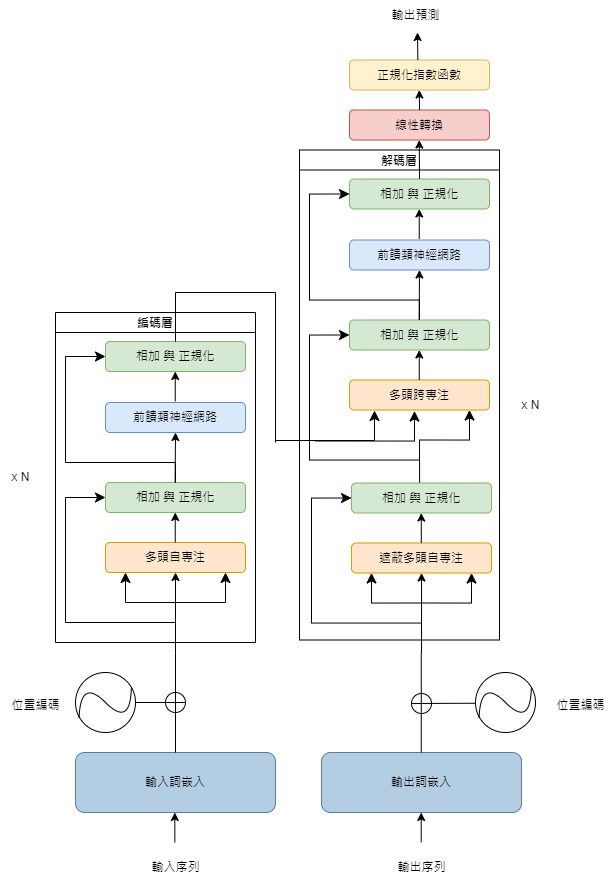
\includegraphics[width=0.9\linewidth]{figures/tfm_arch.drawio.png}
    \caption{轉換器架構圖}
    \label{fig:tfm_arch}
\end{figure}
        由於轉換器不需要對每個時間點逐一運算,使此過程能被高度平行化,類神經網路得以透過專注機制同時進行序列資料的大量訓練。這種可擴展性(Scalability)使其在自然語言和語音處理上取得了巨大的進展,幾乎取代了原先遞迴式類神經網路的應用場景,近年來甚至被應用在圖像類的資料上\cite{dosovitskiy2021image},展現了此種模型架構的彈性與泛用性,成為目前最前沿的人工智慧主流架構。

        除了模型架構,機器學習中不可或缺的另一大部分是對資料的編碼過程。如何更有效率的讓機器理解、處理和輸出資料,是機器學習乃至深層學習的一大課題。面對捉摸不定、抽象且變化萬千的人類語言,語音和文字處理中的表徵學習尤為重要。

\section{表徵與自監督式學習}

\subsection{特徵抽取與表徵學習}

  不論採用何種模型,為了讓機器可以處理並捕捉輸入資料中的訊號與規律,包括如何對資料編碼和運算的步驟,在機器學習中稱之為特徵抽取(Feature Extraction)或表徵學習(Representation Learning),這是模型建構中不可或缺的重要步驟。

        對於抽象的語言概念,早期工程領域根據對語音和文字的理解,分別進行了不同的處理。對於離散且可計數的文字,人們使用詞頻統計衍生出如 \(n\) 連詞(\(n\)-gram)、TF-IDF(詞頻-倒數文件頻率,Term-Frequency Inverse Document Frequency)等特徵作為模型學習的前處理步驟;而對於連續且複雜的語音,工程師則透過聲學原理與訊號處理的知識,使用如濾波器組(Filter Bank)、梅爾倒頻譜係數(Mel-Frequency Cepstrum Coefficient,MFCC)等特徵,類比人耳捕捉語音訊號的過程。

        在深層學習逐漸發展的過程中,自然語言處理領域的一大里程碑是米氏(Mikolov)提出的「Word2vec」模型 \cite{mikolov_efficient_2013},該模型以連續的向量表徵(Vector Representation)取代稀疏(Sparse)的統計數據,對離散的文字單詞進行「詞嵌入(Word Embedding)」編碼。通過大量文本運算,將各單詞之間的共現(Collocation)以跳躍詞(Skip-gram,SG)、連續詞袋(Continuous Bag-of-Word,CBOW)等演算法轉換成高維向量空間中的點,找出每個單詞最適合的語義表徵。爾後,為了更細緻地捕捉同一單詞在不同句子中的脈絡變化,ELMo(來自語言模型的詞嵌入,Embeddings From Language Model)\cite{peters_deep_2018} 提出了「含上下文詞嵌入(Contextualized Embedding)」的概念,使得各單詞在運算表徵的過程中可以根據上下文進行些微調整。

\subsection{自監督學習}

  隨著轉換器模型的提出,BERT(來自轉換器的雙向編碼器表徵,Bidirectional Encoder Representations From Transformers)\cite{devlin_bert_2019} 被提出。通過自專注機制,工程師們無需依賴人工標記,透過預先設定任務(Pretext Task)引導模型從大量文本中自行找出更細緻且考量前後文的語義關係,並在許多文字任務上獲得了優異的成績。

        自此,楊氏(LeCun)將這種以特定任務作為引導、藉助資料本身的結構替代標註,從大量未標註資料中學習資料規律的訓練方式,稱之為「自監督學習(Self-supervised Learning,SSL)」。BERT 的成功使自監督學習得以大行其道,並出現了許多由巨量資料進行預訓練(Pre-train)的基石模型(Foundation Model),有效解決了語言處理領域中的標註資料稀缺的問題。人們在解決語言相關任務時,不需從頭蒐集資料與進行耗時耗能的訓練過程,而是可以利用基石模型優良的泛化(Generalization)能力,解決各種應用任務的需求。相比於預訓練的任務,這些更貼近日常現實的任務被稱為「下游任務(Downstream Task)」,能應對廣泛的下游任務種類,這是基石模型最大的優勢。

        有鑑於文字處理方面的成功,語音領域的研究者嘗試將相似模式應用於語音,眾多語音基石模型隨之出現。大量的語音資料庫幫助模型萃取出有助於下游任務的語音表徵(Speech Representation),在各種任務上獲得了優於傳統聲學特徵的表現。語音表徵具備的無窮潛力,逐漸成為聲學特徵之外的新選擇。

        依照這些語音自監督模型的預訓練學習模式,可大致分為重建式、預測式與對比式模型。以下分別介紹這三類模式:

\subsubsection{重建式學習(Reconstruction Learning)}

  此類模型通過對輸入訊號進行擾動(Perturb)後,期望模型將被更動的輸入重新預測回原始資料,通常減損函數表示為:
\begin{align}
    \mathcal{L}_{recon} = \mathbb{E}_x[|f_\theta(\tilde{x}) - x|]
\end{align}
其中 $\tilde{x}$ 為擾動後的資料,$f_\theta(\cdot)$ 為模型函數。擾動方式通常以遮蔽為主,在文字處理中以 BERT 為代表,稱為「遮蔽語言模型(Masked Language Model,MLM)」。在語音中,採用此方式學習的有 Mockingjay \cite{liu_mockingjay_2019}、TERA \cite{t_tera_2021} 等模型。  % NPC

\subsubsection{預測式學習(Predictive Learning)}

  此類模型通過預訂一些學習目標函數,製造類似輸入與輸出的配對資料,讓模型預測該函數的結果來學習資料中的特定結構。其訓練減損函數可表示為:
\begin{align}
    \mathcal{L}_{pred} = \mathbb{E}_x[\text{eval}(f_\theta(x), \hat{f}(x))]
\end{align}
其中 $\hat{f}$ 是期望模型學習的目標函數,$f_\theta(\cdot)$ 為模型函數,$\text{eval}$ 是用來評估預測好壞的標準。

        目標函數的典型代表是自迴歸(Autoregressive),期望模型預測未來時間點的輸入表徵。文字方面以「GPT(生成式預訓練轉換器,Generative Pretrained Transformer)」系列 \cite{radford_language_nodate, brown_language_2020} 為代表,語音上的「自迴歸預測編碼(Autoregressive Predictive Coding,APC)」 \cite{chung_generative_2020} 也是採用此種模式。此外,語音基石模型還可以使用其他訓練目標,如 PASE+ \cite{ravanelli_multi-task_2020} 預測其他模型的表徵,而本文著重探究的「HuBERT(隱藏單元 BERT,Hidden-unit BERT)」\cite{hsu_hubert_2021, hsu_hubert_2021-2} 則以預測分群(Cluster)後的輸入表徵為目標,這些預測目標又被視為虛擬標註(Pseudo-label),後文將著重探討。

\subsubsection{對比式學習(Contrastive Learning)}

  此學習方式的訓練目標是要求模型區分正樣本(Positive Sample)與負樣本(Negative Sample)的差異,減損函數通常定義為:
\begin{align}
    \mathcal{L}_{contr} = -\mathbb{E}_x\left[\log
        \left(
        {\frac
            {\sum_{\tilde{x} \in x_{pos}}\exp(\text{sim}(x, \tilde{x}))}
            {\sum_{\tilde{x} \in \mathcal{X}}\exp(\text{sim}(x, \tilde{x}))}
        }\right)\right]
\end{align}

        其中 $x$ 為輸入,$x_{pos}$ 為正樣本,$\mathcal{X}$ 為包含正負樣本的資料集,$\text{sim}(\cdot, \cdot)$ 是評估兩個樣本相似程度的函數,常用的相似度函數為內積運算得出的餘弦相似度(Cosine Similarity)。語音上最早使用對比式學習的模型為「對比預測編碼(Contrastive Predictive Coding,CPC)」\cite{maekaku2022speech},之後如 Wav2vec \cite{schneider2019wav2vec}、Modified CPC \cite{rivière2020unsupervised}、Wav2vec 2.0 \cite{baevski2020wav2vec} 等模型亦是以對比正負樣本的模式訓練,但訓練時正負樣本的定義有所差異,如 Wav2vec 僅以時間維度上相同的向量為正樣本,其餘則將固定時間內的向量皆視為正樣本。

        對比式學習通過正負樣本的定義,將預訓練任務形塑為分類問題,因此減損函數本質上為交叉熵,使模型能夠判斷訓練資料中的結構差異。

\subsection{向量量化與離散單元}

  語音訊號雖然記錄語言資訊,卻與影像資料一樣都是連續數值資料,不像離散的文字較易處理,因此發展出了許多應用廣泛的模型。為了使語音模型訓練可以套用自然語言處理領域的演算法,從連續語音中找出離散表徵逐漸成為研究趨勢,這類研究被稱為「聲學單元發掘(Acoustic Unit Discovery,AUD)」。

        由於語言概念本質上是離散符號,向量量化技術常用於涉及語言標註的情境,如電腦視覺經典的量化向量變分自編碼器(Vector-Quantized Variational Autoencoder,VQ-VAE)\cite{van2017neural},利用影像標註的離散語言單詞特性,使模型學習的表徵向量被約束在編碼簿(Codebook) 的幾個向量中。

        在語音領域,基於 Wav2vec 之上的 Vq-wav2vec \cite{baevski2019vq} 和 Wav2vec 2.0 將連續的語音特徵量化加入訓練目標中,在語音辨識等任務上取得了顯著進步。

        HuBERT \cite{hsu_hubert_2021-2} 則先對連續的 MFCC 特徵進行 K-平均(K-Means)演算法分群,以所得的群心(Centroid)或碼字(Code Word)編號作為訓練目標,實施類似 BERT 的遮蔽語言模型訓練,並改以此次訓練得到的語音表徵為目標,再次分群後實施第二次訓練。這些經過兩輪訓練後,從模型表徵分群得到的群心,被視為「隱藏單元(Hidden Unit)」,呈現了語音訊號中的代表性聲學特徵。透過找出隱藏單元的過程,HuBERT 在低資源情況下達到與 Wav2vec 2.0 相近的語音辨識成績。

\subsection{無文字(Textless)架構}

  奠基於 HuBERT 等語音基石模型的成功,利用隱藏單元的概念,將大量語音資料表徵進行 K-平均演算法,作為這些語音訊號的虛擬標註。如此得到的大量離散隱藏單元形成了「虛擬文字(Pseudo-text)」的語料庫,基於這些離散單元訓練的語言模型,稱為「生成式口語語言模型(Generative Spoken Language Model,GSLM)」\cite{lakhotia_generative_2021-1}。配合反向語音合成訓練基於離散單元的語音生成模型,整體架構完全不依賴文字標註,訓練出純語音語言模型,稱為「無文字(Textless)架構」\cite{noauthor_textless_2021}。

        無文字模式在語音問答(Spoken Question Answering)\cite{lin2022dual}和語音到語音翻譯 (Speech-to-speech Translation)\cite{chen_speech--speech_2023}中取得了前所未有的進展。這些「離散單元(Discrete Unit)」被視為類似文字卻不依賴人類文字標記的語音表徵,具有儲存位元率低和可套用文字語言模型訓練模式的優勢,受到語音社群的廣泛借鑑,後續也帶出了許多如\cite{zhang2024speechtokenizer} 等將語音以離散表徵編碼的研究。

        雖然在系統與應用任務上取得了成功,但這些離散單元本身與文字的差異,及其對語音語言模型訓練的幫助,仍是領域內探討的焦點。有鑑於此,本論文基於語言知識,從最接近文字且與語音訊號最相關的「音位(Phoneme)」開始探討,期望了解離散單元能帶來的特徵及其對後續應用的幫助。

\section{本章節總結}

  本章節首先介紹了深層學習模型的核心部件 --- 類神經網路的基本原理,隨後對本論文研究的核心 --- 「語音表徵」與「離散單元」的發展與歷史進行了梳理。接下來的章節將緊扣這些基石模型得到的離散特徵,對其與「音位」這類語音學標記之間的統計關係進行更深入分析。

% \section{相關研究}  

\subsection{無文字與離散語音表徵}

  自 HuBERT 帶起的研究之後,出現了愈來愈多離散表徵相關的研究,例如 \cite{10097097, abdullah23_interspeech, chang_exploration_2023, liu2024dinosr, zhang2024speechtokenizer, huang2023repcodec} 等等。它們在提出自己的離散表徵時,也會採取 HuBERT 的衡量方式,來驗證這些離散單元與語音中的內容及人類對語音的詮釋之間具有一定程度的相關性,並從資訊理論(Information Theory)的角度,證明這些離散單元確實具備區分不同語音資訊的能力。

\subsection{語音學分析}

  由於語音處理本身最終是針對人類語音,因此有一群研究者通過對人類語音的理解,將這些知識應用在分析模型如何對語音訊號建構表徵之上。例如 \cite{deseyssel22_interspeech, wells_phonetic_2022, 10097097, abdullah23_interspeech} 等研究。\par
        基於這些作品對語音離散表徵的興趣和探討,本論文也先透過過往幾個常用來分析語音表徵的方式,特別是HuBERT \cite{hsu_hubert_2021-2} 提出的標準進行初步的分析。

% 
\section{分析結果}

\subsection{基於各自音位的分析}
\begin{table}[!htbp]
    \centering
    \begin{subtable}[t]{\textwidth}
        \centering
        \begin{tabular}{|c|c|c|c|c|c|} \hline
                        & 音位純度   & 分群純度   & 音位熵    & 離散單元熵  & PNMI   \\ \hline
            HuBERT      & 0.5256 & 0.3382 & 3.3152 & 3.8681 & 0.4993 \\ \hline    %% 1.6552 h
            Wav2vec 2.0 & 0.4006 & 0.2676 & 3.3152 & 3.8215 & 0.3706 \\ \hline    %% 1.2286 w
            CPC         & 0.5188 & 0.3812 & 3.3146 & 3.7918 & 0.4992 \\ \hline    %% 1.6545 c
            LogMel      & 0.3253 & 0.1473 & 3.3158 & 3.8630 & 0.2647 \\ \hline    %% 0.8776 l 
        \end{tabular}
        \caption{群數 = 50}
        \label{tab:ch3-clu050-phn}
    \end{subtable}

    \vspace{0.5cm}

    \begin{subtable}[t]{\textwidth}
        \centering
        \begin{tabular}{|c|c|c|c|c|c|} \hline
                        & 音位純度   & 分群純度   & 音位熵    & 離散單元熵  & PNMI   \\ \hline
            HuBERT      & 0.6097 & 0.2553 & 3.3152 & 4.5704 & 0.5786 \\ \hline    %% 1.9181 h
            Wav2vec 2.0 & 0.4877 & 0.2118 & 3.3152 & 4.5284 & 0.4596 \\ \hline    %% 1.5235 w
            CPC         & 0.5895 & 0.2674 & 3.3146 & 4.5034 & 0.5557 \\ \hline    %% 1.8418 c
            LogMel      & 0.3348 & 0.0931 & 3.3158 & 4.5591 & 0.2789 \\ \hline    %% 0.9247 l 
        \end{tabular}
        \caption{群數 = 100}
        \label{tab:ch3-clu100-phn}
    \end{subtable}

    \vspace{0.5cm}

    \begin{subtable}[t]{\textwidth}
        \centering
        \begin{tabular}{|c|c|c|c|c|c|} \hline
                        & 音位純度   & 分群純度   & 音位熵    & 離散單元熵  & PNMI   \\ \hline
            HuBERT      & 0.6474 & 0.1644 & 3.3152 & 5.2681 & 0.6289 \\ \hline    %% 2.0849 h
            Wav2vec 2.0 & 0.5427 & 0.1467 & 3.3152 & 5.2173 & 0.5188 \\ \hline    %% 1.7199 w
            CPC         & 0.6098 & 0.1789 & 3.3146 & 5.1885 & 0.5882 \\ \hline    %% 1.9497 c
            LogMel      & 0.3474 & 0.0569 & 3.3158 & 5.2322 & 0.2955 \\ \hline    %% 0.9798 l 
        \end{tabular}
        \caption{群數 = 200}
        \label{tab:ch3-clu200-phn}
    \end{subtable}

    \caption{不同群數在四種基石模型的音位分析數據}
    \label{tab:single-cluster-results}
\end{table}
  由表 \ref{tab:single-cluster-results} 中可以看出,分群的群數愈多時,音位的純度確實有所上升,但這可能是犧牲分群純度得來的。因此再看 PNMI 的指標可以發現,整體離散單元和音位標註的相關性還是有所提升的。此外,從不同模型來觀察,HuBERT 的表現是四種語音表徵中最好的,一定程度上可以證實 HuBERT 在找出語音中有意義單位上的效能,及其為什麼無文字架構通常以 HuBERT 作為抽取語音離散表徵的模型。

\subsection{基於語音學分類的分析}
\begin{table}[!htbp]
    \centering
    \begin{subtable}[t]{\textwidth}
        \centering
        \begin{tabular}{|c|c|c|c|c|c|} \hline
                        & 標註純度   & 分群純度   & 標註熵    & 離散單元熵  & NMI    \\ \hline
            HuBERT      & 0.7466 & 0.1422 & 1.7530 & 3.8681 & 0.5742 \\ \hline    %% h  1.0065
            Wav2vec 2.0 & 0.6913 & 0.1570 & 1.7530 & 3.8215 & 0.4682 \\ \hline    %% w  0.8208
            CPC         & 0.7418 & 0.1953 & 1.7530 & 3.7918 & 0.5644 \\ \hline    %% c  0.9894
            LogMel      & 0.5980 & 0.0953 & 1.7530 & 3.8630 & 0.3403 \\ \hline    %% l  0.5966 
        \end{tabular}
        \caption{群數 = 50}
        \label{tab:ch3-clu050-pcls}
    \end{subtable}

    \vspace{0.2cm}

    \begin{subtable}[t]{\textwidth}
        \centering
        \begin{tabular}{|c|c|c|c|c|c|} \hline
                        & 標註純度   & 分群純度   & 標註熵    & 離散單元熵  & NMI    \\ \hline
            HuBERT      & 0.7804 & 0.0856 & 1.7530 & 4.5704 & 0.6148 \\ \hline    %% h  1.0778
            Wav2vec 2.0 & 0.7219 & 0.0889 & 1.7530 & 4.5284 & 0.5252 \\ \hline    %% w  0.9207
            CPC         & 0.7790 & 0.0997 & 1.7530 & 4.5034 & 0.6046 \\ \hline    %% c  1.0599
            LogMel      & 0.6032 & 0.0567 & 1.7530 & 4.5591 & 0.3512 \\ \hline    %% l  0.6157 
        \end{tabular}
        \caption{群數 = 100}
        \label{tab:ch3-clu100-pcls}
    \end{subtable}

    \vspace{0.2cm}

    \begin{subtable}[t]{\textwidth}
        \centering
        \begin{tabular}{|c|c|c|c|c|c|} \hline
                        & 標註純度   & 分群純度   & 標註熵    & 離散單元熵  & NMI    \\ \hline
            HuBERT      & 0.8004 & 0.0464 & 1.7530 & 5.2681 & 0.6563 \\ \hline    %% h  1.1504
            Wav2vec 2.0 & 0.7490 & 0.0527 & 1.7530 & 5.2173 & 0.5671 \\ \hline    %% w  0.9941
            CPC         & 0.7947 & 0.0644 & 1.7530 & 5.1885 & 0.6345 \\ \hline    %% c  1.1123
            LogMel      & 0.6107 & 0.0335 & 1.7530 & 5.2322 & 0.3652 \\ \hline    %% l  0.6401 
        \end{tabular}
        \caption{群數 = 200}
        \label{tab:ch3-clu200-pcls}
    \end{subtable}

    \caption{不同群數在四種基石模型按照語音學類別的分析數據}
    \label{tab:single-cluster-phonetype-results}
\end{table}
  將表 \ref{tab:single-cluster-phonetype-results} 與音位的表 \ref{tab:single-cluster-results} 進行比較,能看出音位數據表現的趨勢,也能在語音類別中看出來。然而,由於語音類別數明顯少於音位的種類數,因此語音類別標註的純度相較音位會較高。

\setcounter{section}{4}
\section{分析結果}

\begin{figure}
    \centering
    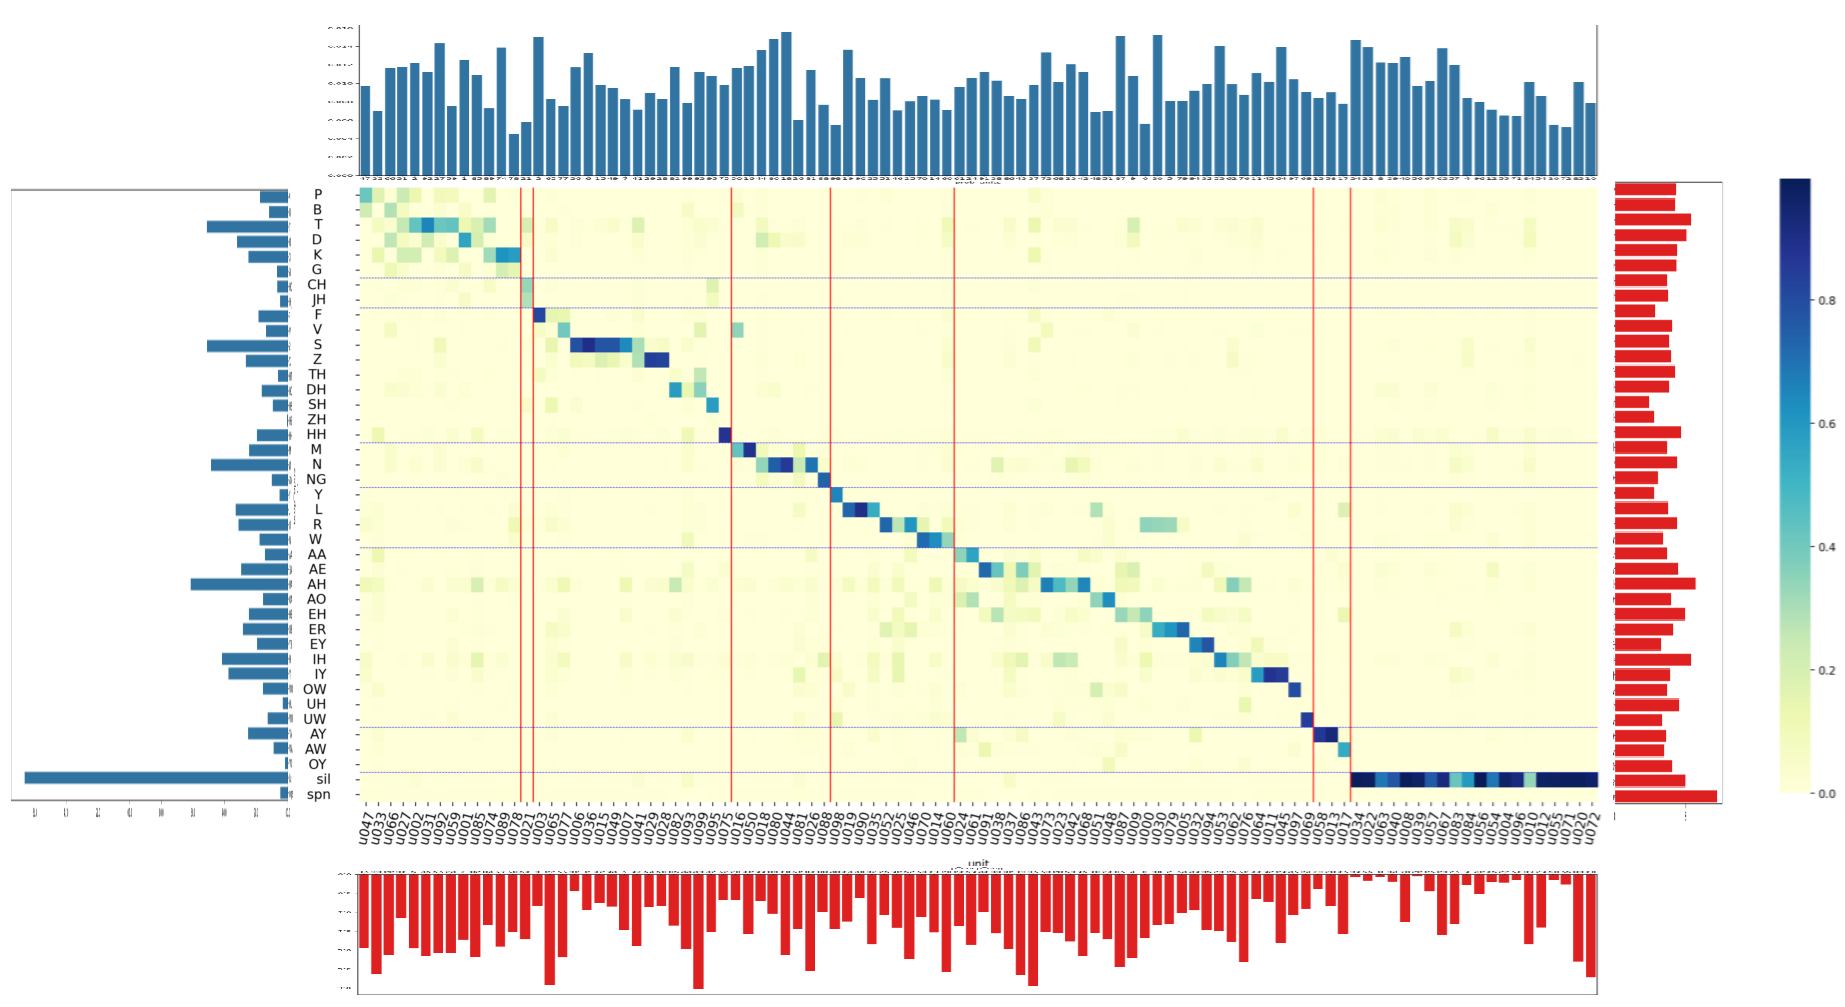
\includegraphics[width=1\linewidth]{figures/better__p_ph_given_un.png}
    \caption{HuBERT 100}
    \label{p_p_given_u-hub-100}
\end{figure}

  為了更直觀的了解模型離散單元與音素之間的對應關係,接下來的分析將把音素與單元的聯合分佈 \(p(p|u)\) 作圖呈現,如 \ref{p_p_given_u-hub-100} 所示。以下說明這張圖表的看法:\par
       橫軸是各單元,而縱軸是各音素,按照發音分組方式,輔音遵循國際音標的圖表排列,元音則按照 ARPABET (cite CMU Dict) 字母順序排列。由於離散單元編號本身並無特殊含義,因此當單元數太多時將省略。\par
       為了更好的看出各組別之間的關係,圖表上先將各組之間以橫線區分。按照語音學分組後,為了考慮單元之間的代表性,將每個單元都找出相對應最高機率的音素,接著將每個單元亦依照對應音素在縱軸的排列順序一一排列,若是遇到對應同一音素的兩種離散單元,則以 \(p(u|p) \) 由高至低排列。最後再橫軸上也以語音學分組區分。\par
       如此一來,便能夠呈現出一張由左上至右下的對應圖。這張圖在 (cite DinoSR) 等 paper 也有呈現。從圖中可以看出,用來編碼 sil 的 unit 其實佔據了不小的部分。

\mychcnt{3}
\chapter{單一語音離散表徵與音位的關係}

% 
{  % 單一語音離散表徵與音位的關係

  HuBERT \cite{hsu_hubert_2021, hsu_hubert_2021-2} 和 Wav2vec 2.0 \cite{baevski2020wav2vec} 等語音基石模型的成功,不僅在語音任務上達到了前所未有的表現,還促進了語音表徵離散化的發展。由此產生的「無文字(Textless)」架構 \cite{noauthor_textless_2021, lakhotia_generative_2021, lakhotia_generative_2021-1},讓人們在處理語音訊號時,有了連續表徵以外的新選擇。離散形式的表徵可以直接應用文字領域發展的技術,如機器翻譯、生成式模型等,為語音技術帶來新的突破。另一方面,基於離散「符記(Token)」的共同形式,離散語音表徵可以更好的整合文字資料,促成多模態領域的發展。跨模態離散表徵的成功,甚至驅使影像領域也開始發展離散表徵,\jeffcomment{\textcolor{yellow}{(要確認一下「開始」嗎?)}}如探討唇語的 AV-HuBERT \cite{shi2021learning} 等等,展現了離散表徵在資料處理上的優勢。

        此外,除了技術的角度切入,這樣的技術也可以探討離散語音表徵成功背後的可能因素,以及它們與語言學對人類語音理解之間的差異,甚至是進一步利用這些技術協助更細緻的探討人類的語音現象。因此,原先在連續語音表徵上的語音學分析,也開始關注離散表徵在多大程度上能描述語音現象,將其列入考量,成為除了連續語音特徵和時頻譜之外的另一個選擇。

}  % 單一語音離散表徵與音位的關係

\section{相關研究}  

\subsection{無文字與離散語音表徵}

  自 HuBERT 帶起的研究之後,出現了愈來愈多離散表徵相關的研究\cite{10097097, abdullah23_interspeech, chang_exploration_2023, liu2024dinosr, zhang2024speechtokenizer, huang2023repcodec} 。它們在提出自己的離散表徵時,也會採取 HuBERT 的衡量方式,來驗證這些離散單元與語音中的內容及人類對語音的詮釋之間,具有一定程度的相關性,並從資訊理論(Information Theory)的角度,證明這些離散單元確實具備區分不同語音資訊的能力。

\subsection{語音學分析}

  由於語音處理本身最終是針對人類語音,因此有一群研究者通過對人類語音的理解,將這些知識應用在分析模型如何對語音訊號建構表徵之上\cite{deseyssel22_interspeech, wells_phonetic_2022, 10097097, abdullah23_interspeech} 。基於這些作品對語音離散表徵的興趣和探討,本論文也先透過過往幾個常用來分析語音表徵的方式,特別是HuBERT \cite{hsu_hubert_2021-2} 提出的標準進行初步的分析。


\section{衡量方式}

  本次研究主要探討純度(Purity)、熵(Entropy)和相互資訊(Mutual Information,MI)等指標,這些指標在 HuBERT 中被採用 \cite{hsu_hubert_2021, hsu_hubert_2021-2},用以比對機器學習過程中得到的虛擬標註與人類標註之間的相關性(Correlation)。以下對各標準進行詳細解釋:

        不論是何種語音基石模型,語音表徵的基本單位是音框(Frame)。因此一段語句(Utterance)的語音離散單元被表示為 $[y_1, \cdots\cdots, y_T]$。其中 $T$ 是該段語句的音框總數。對於該段語句,若給予一段在音框上對齊的音素標註(Phonetic Label) $[z_1, \cdots\cdots, z_T]$,此時我們可以將離散單元與標註之間配對的出現次數,寫為一個雙變數的共同分佈(Joint Distribution)
\begin{align}
    p_{yz} = \frac{\sum^T_{t=1}[{y_t = i \wedge z_t = j}]}{T}
\end{align}

其中 $i$ 是第 $i$ 個音位類別,而 $j$ 指編號為$j$的離散單元。兩個變數的邊際機率(Marginal Probability)分別為
\begin{align}
    p_z(j) & =\sum_i{p_{yz}(i, j)} \\
    p_y(i) & =\sum_j{p_{yz}(i, j)}
\end{align}
因此,對於每一個音位 $i$ 而言,這個音位最可能的對應離散單元為
\begin{align}
    z^\ast(i) = \arg\max_j p_{yz}(i, j)
\end{align}
與之相對應的,對於每一個離散單元的類別 $j$ 則可以找到機率最高的音位
\begin{align}
    y^\ast(j) = \arg\max_i p_{yz}(i,j)
\end{align}
透過這些定義,以下分節介紹將要用來分析的指標:

\subsection{純度}

  本指標考慮音位和離散單元兩個序列之間對應的最高機率,因此從音位與離散單元的角度出發,可以得到以下兩項數據:

\paragraph{音位純度(Phoneme Purity)}\hfill \break
%
        考慮每個離散單元對應的音位中,最高機率音位的機率,表示為
\begin{align}
    \mathbb{E}_{p_z(j)}\left[p_{y|z}(y^*(j)|j) \right]
\end{align}
此指標表示該單元是否對其對應的音位有足夠的代表性。

\paragraph{分群純度(Cluster Purity)}\hfill \break
%
        與音位純度相對,改以每個音位的角度,考慮對應單元類別的機率
\begin{align}
    \mathbb{E}_{p_y(i)}\left[p_{z|y}(z^*(i)|i) \right]
\end{align}
        由於離散表徵進行分群演算法時的類別數是一項超參數(Hyperparameter),且通常離散單元的分群數量會比音位多,因此該統計數據本身不直接具有語音學的解釋意義,而且在分群數量很多時其數值會顯著下降。然而該指標在考量音位純度時必須一併考慮,因為當分群數非常多時,分群純度過低暗示離散單元做不到歸納音位類別的效果,使得音位純度失去其意義。一個極端的情形是每一個音框都給予不同的離散單元編號,如此音位純度可以達到100\%。

\subsection{熵和相互資訊}

  除了純度提供「最高機率」的對應關係,根據 HuBERT 論文 \cite{hsu_hubert_2021-2} 中的分析方式,我們也可以從資訊理論的角度,觀察兩個序列的熵和相互資訊。

\paragraph{熵(Entropy)} \hfill \break
%
  熵的定義按照資訊理論,衡量兩個序列中標籤類別出現機率的不確定性(Uncertainty),公式寫作:
\begin{align}
    H(y) & = \sum_i{p_y(i)\log p_y(i)} \\
    H(z) & = \sum_j{p_z(j)\log p_z(j)}
\end{align}
其中 $H(y)$ 和 $H(z)$ 分別為音位和離散單元的熵,數值愈高分別表示各種音位和離散單元出現的機率愈平均。

\paragraph{以音位標準化之相互資訊(Phone-normalized Mutual Information,PNMI)}\hfill \break
%
  本數據以「觀察到某一個離散單元,能降低多少音位標註的不確定性」,定義該離散單元的出現背後提供了多少音位的資訊。公式寫為:
\begin{align}
    \frac{I(y;z)}{H(y)} & =\cfrac{\sum_i \sum_j p_{yz}(i, j) \log \cfrac{p_{yz}(i, j)}{p_y(i)p_z(j)}}{\sum_i p_y(i) \log p_y(i)} \\
                        & =\frac{H(y)-H(y|z)}{H(y)}                                                                              \\
                        & =1-\frac{H(y|z)}{H(y)}
\end{align}
        該項數據愈高,表示離散單元的分群愈能提供語音音位的資訊,是一個品質更好的分群結果。由於離散單元是否能夠正確對應到音位才是人們所關心的問題,因此與純度不同,只以音位的角度出發,而不考慮以離散單元分群的角度。

\section{語音學的音位分類(Phoneme Type)}

  除了單一音位本身的特性以外,由於音位之間存在相似的特徵,可以分成幾個組別。這裡依照希氏(Sicherman) \cite{10097097}、阿氏(Abdullah)\cite{abdullah23_interspeech} 等前作的分組方式,對英語的音位進行分類並合併比對數據,觀察這些離散單元是否有擷取到相似的發聲特徵,而不單純只是把音位分成約 50 類完全獨立的標籤。以下簡介六個音位組別:
        
        \begin{itemize}
            \item 塞音(Plosive):以完全阻塞氣流的方式發音的音位,包含 /p/、/b/、/t/、/d/、/k/、/g/ 六種
            \item 擦音(Fricative):藉由在口腔中形成的縫隙,使氣流通過時摩擦形成的發音,包含 /f/、/v/、/s/、/z/、/\textesh/ (sh)、/\textyogh/ (如「garage」的 「-ge」)、/θ/ (無聲的 th)、/ð/ (有聲的 th)、/h/ 九種
            \item 塞擦音(Affricate):由塞音和同部位的擦音同時發出的輔音,英語中只有 /t\textesh/ 和 /d\textyogh/ 兩種,即 ch 和 j 的發音
            \item 鼻音(Nasal):使氣流通過鼻腔形成的聲音,有 /m/、/n/、/ŋ/ (ng) 三種
            \item 近音(Approximant):又稱半元音,為介於元音和輔音之間的聲音,有 /j/ (為 y 作為輔音時的發音)、/r/、/l/、/w/
            \item 元音(Vowel):可自成音節的音位,包含發音位置固定的單元音(Monophthong)和會移動的的雙元音(Diphthong),通常以 a、e、i、o、u 字母產生的聲音皆屬於此類別
        \end{itemize}
        
        透過將音位分組後,形成新的語音標註,並重新分析統計指標,觀察在純度等數據是否顯示離散單元與語音的發音方式具有更明確的關聯性。


\section{實驗集與分析模型}

  本研究的分析對象參考無文字架構 \cite{noauthor_textless_2021, lakhotia_generative_2021, lakhotia_generative_2021-1} 的研究,
採用論文中提及的四種語音表徵,簡述如下:

\begin{itemize}
    \item CPC:卷積式編碼器 + 遞迴式預測器,以對比式學習訓練。表徵來自預測器的中間層,每 10 毫秒提取一個向量表徵作為音框
    \item Wav2vec 2.0:卷積式編碼器 + 轉換器預測器,以對比式學習訓練。表徵來自轉換器第 14 層,每 20 毫秒作為一個音框
    \item HuBERT:卷積式編碼器 + 轉換器預測器,以預測式學習訓練,其訓練目標為 K-平均分群演算法的結果,透過遮蔽語言模型的方式訓練。表徵來自轉換器第 6 層,每 20 毫秒作為一個音框
    \item LogMel:為 80 維對數梅爾時頻譜的聲學特徵,在此作為比較基線(Baseline)。音框寬度為 10 毫秒
\end{itemize}

        我們使用該論文\textcolor{red}{(哪一篇?)}釋出之預訓練模型與 K-平均量化模型。預訓練模型細節詳述於 \cite{lakhotia_generative_2021-1} 中,量化模型則是該篇論文透過公開的 LibriSpeech 資料集 \cite{panayotov_librispeech_2015} 中 train-clean-100 訓練集,獲取語音表徵後執行 K-平均分群演算法所得,並釋出群數為 50、100 和 200 的三個版本。

        本論文以 LibriSpeech train-clean-100 作為分析對象,將語音語料庫的語音資料經過四個模型獲取連續表徵後,再經過量化模型得到完全由離散單元組成的「虛擬文字」語料。

        本論文針對語音學的音位標註,透過強迫對齊器(Forced-aligner)\footnote{https://github.com/MontrealCorpusTools/Montreal-Forced-Aligner}的英語預訓練模型,從語料庫的文字轉寫取得語音資料的音位標註與對應的時間範圍。最後透過語音表徵各自的時間解析度生成以音框為單位的音位標註語料。最後將兩者對語音資料集進行音位標註相關性的分析。

% 
\setcounter{section}{4}

\section{分析結果 (New)}

\input{chapters/d___ch3Figs1}

  為了更直觀的了解模型離散單元與音素之間的對應關係,接下來的分析將把音素與單元的聯合分佈 \(p(p|u)\) 作圖呈現,如 \ref{p_p_given_u-hub-100} 所示。以下說明這張圖表的看法:

        橫軸是各單元,而縱軸是各音素,按照發音分組方式,輔音遵循國際音標的圖表排列,元音則按照 ARPABET (cite CMU Dict) 字母順序排列。由於離散單元編號本身並無特殊含義,因此當單元數太多時將省略。

        為了更好的看出各組別之間的關係,圖表上先將各組之間以橫線區分。按照語音學分組後,為了考慮單元之間的代表性,將每個單元都找出相對應最高機率的音素,接著將每個單元亦依照對應音素在縱軸的排列順序一一排列,若是遇到對應同一音素的兩種離散單元,則以 \(p(u|p) \) 由高至低排列。最後再橫軸上也以語音學分組區分。

        如此一來,便能夠呈現出一張由左上至右下的對應圖。這張圖在 (cite DinoSR) 等 paper 也有呈現。從圖中可以看出,用來編碼 sil 的 unit 其實佔據了不小的部分。

\setcounter{section}{4}

\section{分析結果}

\subsection{基於各自音位的分析}

\input{tables/chapter3/chapter3-5.ztable1}

  由表 \ref{tab:single-cluster-results} 中可以看出,分群的群數愈多時,音位的純度確實有所上升,但這可能是犧牲分群純度得來的。因此再看 PNMI 的指標可以發現,整體離散單元和音位標註的相關性還是有所提升的。此外,從不同模型來觀察,HuBERT 的表現是四種語音表徵中最好的,一定程度上可以證實 HuBERT 在找出語音中有意義單位上的效能,及其為什麼無文字架構通常以 HuBERT 作為抽取語音離散表徵的模型。

\textcolor{red}{(討論太少應增加尤應增加舉例分析(某一 phoneme 對應到哪些 unit,它們如何分散或集中,不是只看平均值))}

\subsection{基於語音學及其音位分類的分析}

\input{tables/chapter3/chapter3-5.ztable2}

  將表 \ref{tab:single-cluster-phonetype-results} 與音位的表 \ref{tab:single-cluster-results} 進行比較,能看出音位數據表現的趨勢,也能在語音類別中看出來。然而,由於語音類別數明顯少於音位的種類數,因此語音類別標註的純度相較音位會較高。

\textcolor{red}{同樣太少討論,應增加尤其已有 3.3 的分類,尤可依據其 3.3 的類來分析}

\section{本章總結}

  本章節探討以音框為單位取出的語音離散表徵與對應的音位標註之間的關係,從分析結果中可以看到,HuBERT 模型的離散表徵確實與人類理解的語音單位「音位」之間具有最明顯的相似性,也進一步證明為何 HuBERT 是抽取語音離散表徵時最常使用的模型。

        然而,單一離散表徵僅能代表 10 或 20 毫秒的語音訊號,而音位的長度經常佔據不只一個離散表徵。因此,下一章節將進一步組合多個離散表徵成為符記,分析它們與音位之間的關係。

{
{  % \section{model 之間的比較}
% \subsection{個案分析}
% \subsection{分析結果}
% \subsection{本章總結}
} % \section{model、個案}
{  % 單一語音離散表徵與音位的關係

  HuBERT \cite{hsu_hubert_2021, hsu_hubert_2021-2} 和 Wav2vec 2.0 \cite{baevski2020wav2vec} 等語音基石模型的成功,不僅在語音任務上達到了前所未有的表現,還促進了語音表徵離散化的發展。由此產生的「無文字(Textless)」架構 \cite{noauthor_textless_2021, lakhotia_generative_2021, lakhotia_generative_2021-1},讓人們在處理語音訊號時,有了連續表徵以外的新選擇。離散形式的表徵可以直接應用文字領域發展的技術,如機器翻譯、生成式模型等,為語音技術帶來新的突破。另一方面,基於離散「符記(Token)」的共同形式,離散語音表徵可以更好的整合文字資料,促成多模態領域的發展。跨模態離散表徵的成功,甚至驅使影像領域也開始發展離散表徵,\jeffcomment{\textcolor{yellow}{(要確認一下「開始」嗎?)}}如探討唇語的 AV-HuBERT \cite{shi2021learning} 等等,展現了離散表徵在資料處理上的優勢。

        此外,除了技術的角度切入,這樣的技術也可以探討離散語音表徵成功背後的可能因素,以及它們與語言學對人類語音理解之間的差異,甚至是進一步利用這些技術協助更細緻的探討人類的語音現象。因此,原先在連續語音表徵上的語音學分析,也開始關注離散表徵在多大程度上能描述語音現象,將其列入考量,成為除了連續語音特徵和時頻譜之外的另一個選擇。

}  % 單一語音離散表徵與音位的關係
\section{相關研究}  

\subsection{無文字與離散語音表徵}

  自 HuBERT 帶起的研究之後,出現了愈來愈多離散表徵相關的研究\cite{10097097, abdullah23_interspeech, chang_exploration_2023, liu2024dinosr, zhang2024speechtokenizer, huang2023repcodec} 。它們在提出自己的離散表徵時,也會採取 HuBERT 的衡量方式,來驗證這些離散單元與語音中的內容及人類對語音的詮釋之間,具有一定程度的相關性,並從資訊理論(Information Theory)的角度,證明這些離散單元確實具備區分不同語音資訊的能力。

\subsection{語音學分析}

  由於語音處理本身最終是針對人類語音,因此有一群研究者通過對人類語音的理解,將這些知識應用在分析模型如何對語音訊號建構表徵之上\cite{deseyssel22_interspeech, wells_phonetic_2022, 10097097, abdullah23_interspeech} 。基於這些作品對語音離散表徵的興趣和探討,本論文也先透過過往幾個常用來分析語音表徵的方式,特別是 HuBERT \cite{hsu_hubert_2021-2} 提出的標準進行初步的分析。


\section{衡量方式}

  本次研究主要探討純度(Purity)、熵(Entropy)和相互資訊(Mutual Information,MI)等指標,這些指標在 HuBERT 中被採用 \cite{hsu_hubert_2021, hsu_hubert_2021-2},用以比對機器學習過程中得到的虛擬標註與人類標註之間的相關性(Correlation),接下來將詳細解釋這些指標的定義。

        包含聲學特徵與語音基石模型,不論採用何種方式獲得語音表徵,語音訊號皆是以音框(Frame)為基本單位進行處理。具體而言,給予一段聲音訊號,語音處理系統會將這段訊號按照固定時間切割成多個片段分別處理,這些片段的長度被稱之為時間解析度(Time Resolution)。因此,對於任意一段語句(Utterance),系統會將訊號轉換成一連串的向量 $\boldsymbol{x} = [x_1, \cdots\cdots, x_T]$ 作為語音表徵,其中 $T$ 是該段語句的音框總數,與該語句的時長成比例。其中,第 $t$ 個向量 \(x_t\) 表示第 $t$ 個音框的語音訊號內容。在離散表徵的研究中,每個語音表徵向量 $x_t$ 透過向量量化(Vector Quantization)程序,對應到編碼簿中的某個碼字 $e_{z_t}$。因此,該段語句將被表示為 $\boldsymbol{z} = [z_1, \cdots\cdots, z_T]$ 的離散單元序列。

        與此對應,藉由強迫對齊器(Forced-Aligner)或人工標註,可以獲得該段語句的音素標註(Phonetic Label)。然而,通常音素標註是以每個音位的起始至終止的時間點配上此時間段的音位類別呈現。因此,為了配合語音表徵對語句的處理方式,這段音素標註會被依照時間點對應的範圍在音框上對齊,成為 $\boldsymbol{y} = [y_1, \cdots\cdots, y_T]$ 的形式以便分析與後續處理。

        為方便具體說明,吾人從語音常用的 LibriSpeech \cite{panayotov_librispeech_2015} 公開資料集中取一段音檔\footnote{取自 train-clean-100 訓練子集,編號 89-218-0056,即編號 89 語者在章節編號 218 中第 56 句。},放上波形與音框的對照在圖 \ref{fig:enter-labelwav} 呈現。 該段語句內容為 "... what means could it..." ,上方兩個橫列為單詞標註、音位標註 \footnote{ARPABet 表示法,是以純字母表示的音位表示法}。接下來四個橫列中,可以看見第三與第五個橫列將語句切割成以 20 毫秒為單位的片段,此即前面所述之音框。第三列為 HuBERT 模型分群數 100 所得之離散單元序列,而第五列則是由第二列的音位標註片段按照所對應的時間段,分別對齊到音框上的音素標註。由於音位的長度通常長於一個音框,因此在離散單元和音框音素標註在呈現上習慣將標註類別相同的音框合在一起成為長短不一但更接近時間發音的時間段,分別標在第四與第六列之上。
        \begin{figure}
            \centering
            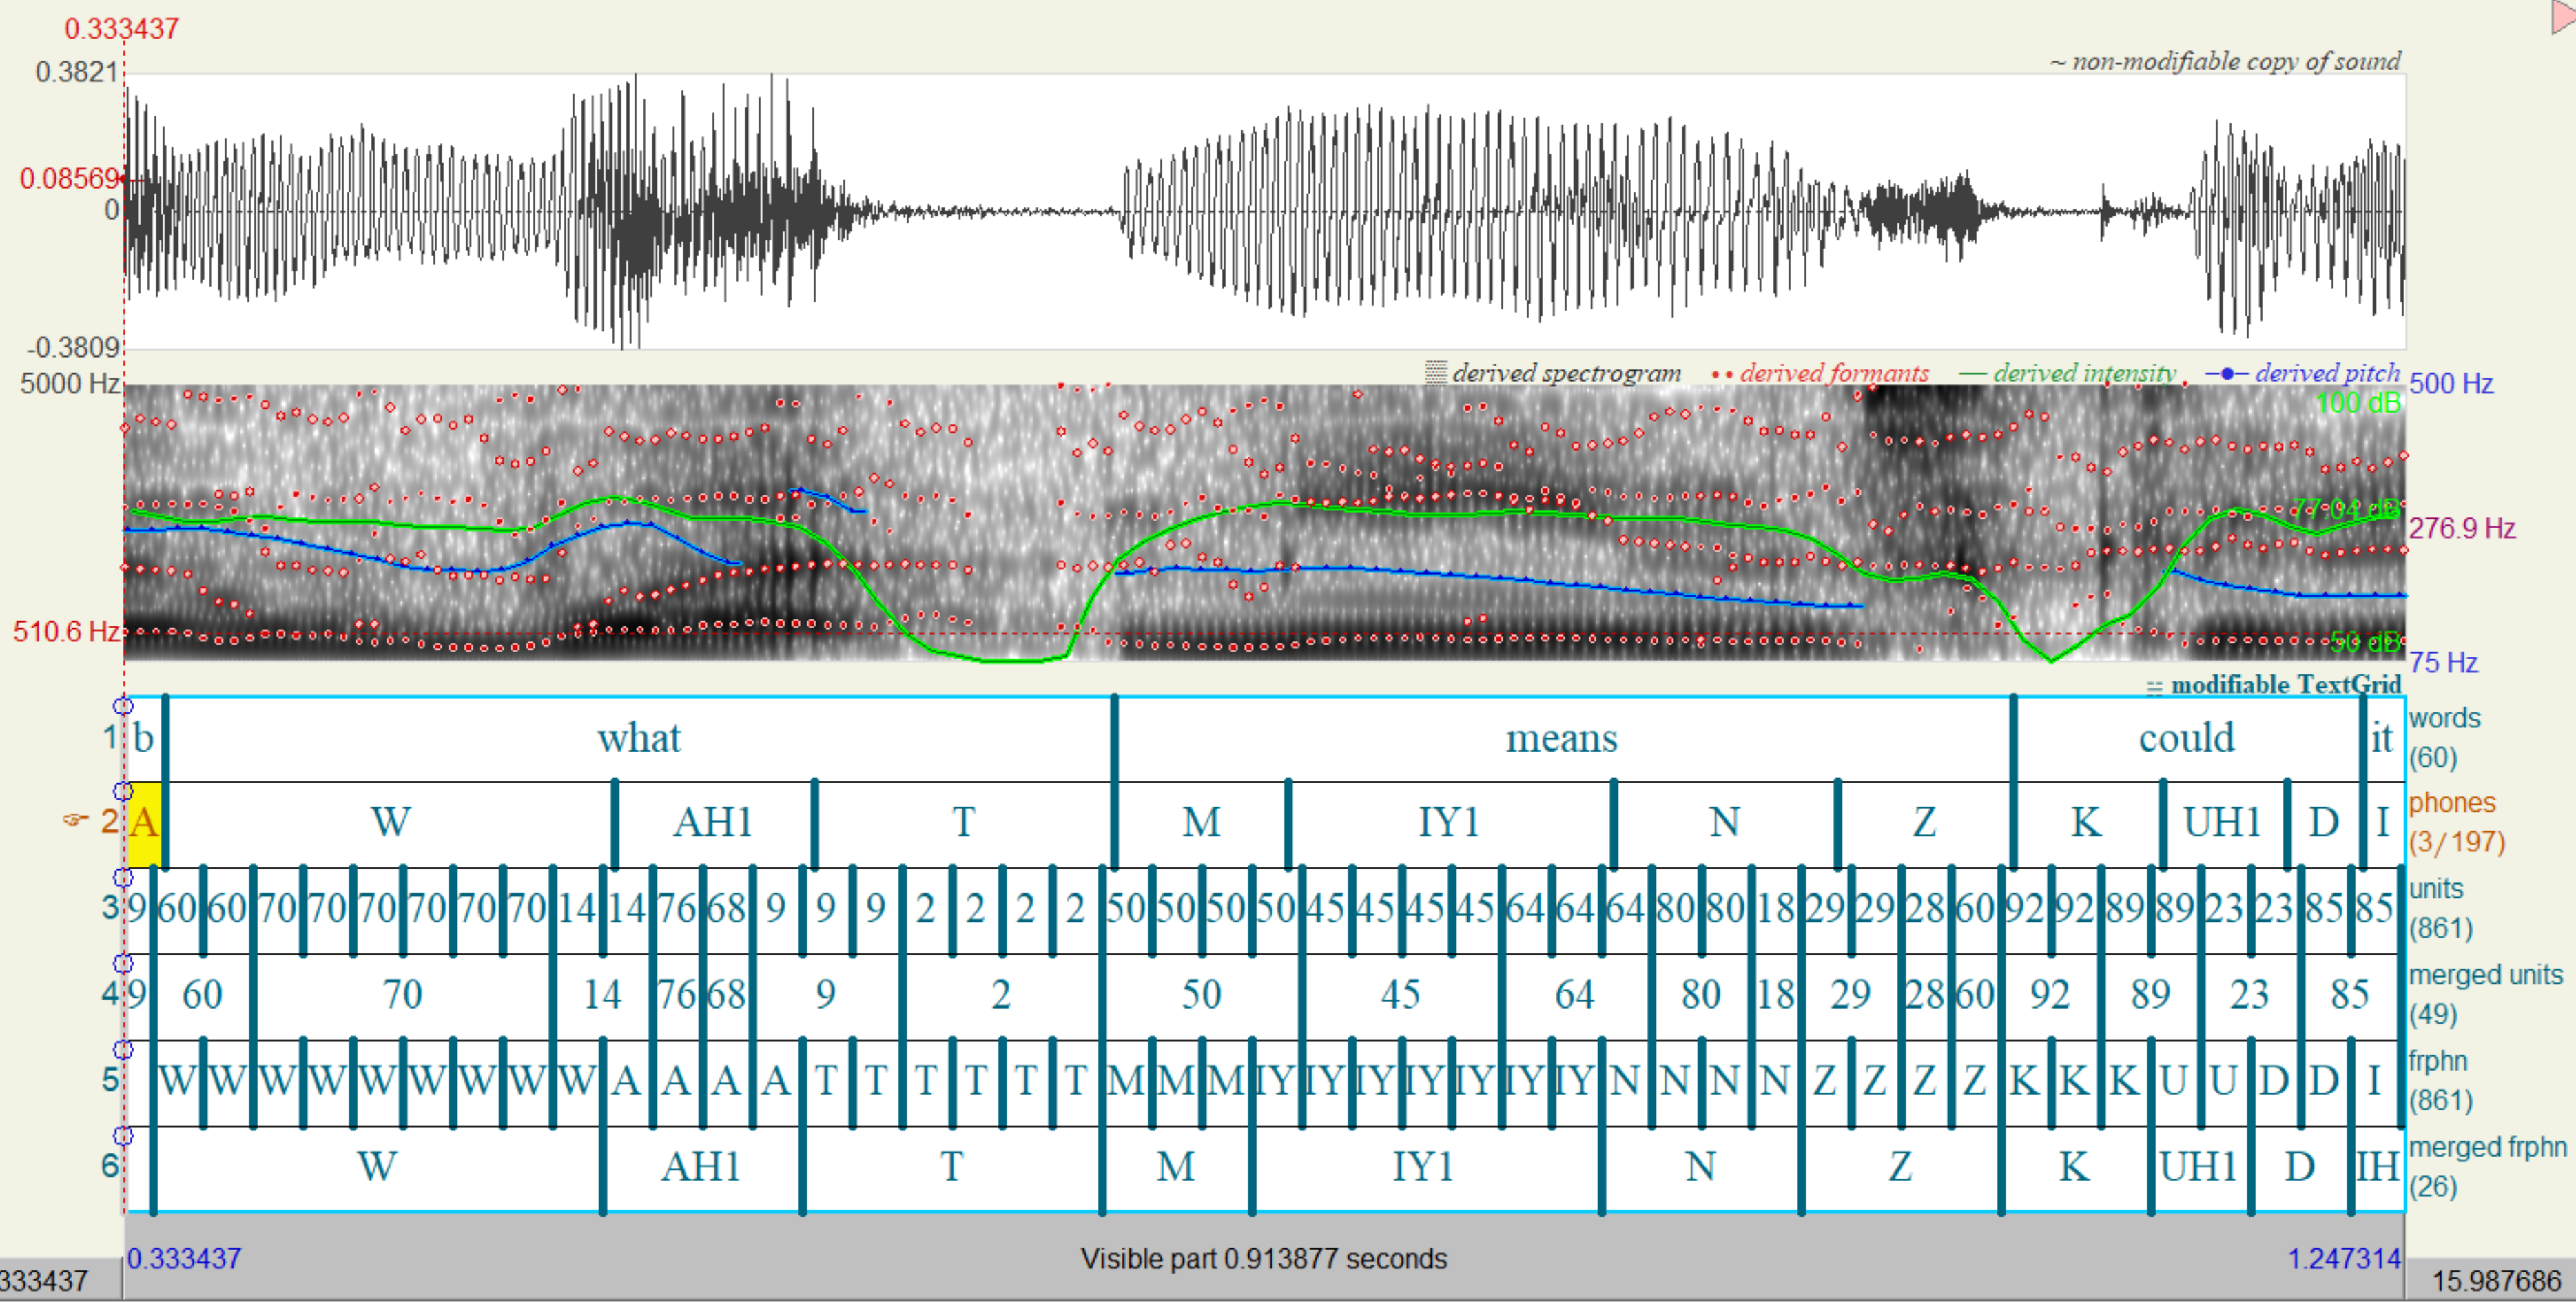
\includegraphics[width=1\linewidth]{figures/praat.png}
            \caption{以音框對齊的離散單元與音素標註範例}
            \label{fig:enter-labelwav}
        \end{figure}
        %%%%%%%%%%%%%%%%%
        
        此時若將整個待分析資料集的語音訊號全部蒐集起來,一共有 $T'$ 個音框,如此可分別獲得一個離散單元序列 $\boldsymbol{z} = \{z_t\}_{t=1}^{T'}$ 與音素標註序列 $\boldsymbol{y} = \{y_t\}_{t=1}^{T'}$ 進行統計分析。我們可以根據離散單元與標註之間配對的出現次數,寫為一個雙變數的共同分佈(Joint Distribution)
\begin{align}
    p_{yz} = \frac{\sum^{T'}_{t=1}[{y_t = i \wedge z_t = j}]}{T'}
\end{align}

其中 $i$ 是第 $i$ 個音位類別,而 $j$ 指編號為 $j$ 的離散單元。兩個變數的邊際機率(Marginal Probability)分別為
\begin{align}
    p_z(j) & =\sum_i{p_{yz}(i, j)} \\
    p_y(i) & =\sum_j{p_{yz}(i, j)}
\end{align}
因此,對於每一個音位 $i$ 而言,這個音位最可能的對應離散單元為
\begin{align}
    z^\ast(i) = \arg\max_j p_{yz}(i, j)
\end{align}
與之相對應的,對於每一個離散單元的類別 $j$ 則可以找到機率最高的音位
\begin{align}
    y^\ast(j) = \arg\max_i p_{yz}(i,j)
\end{align}
透過這些定義,以下分節介紹將要用來分析的指標。

\subsection{純度}

  本指標考慮音位和離散單元兩個序列之間對應的最高機率,因此從音位與離散單元的角度出發,可以得到以下兩項數據:

\paragraph{音位純度(Phoneme Purity)}\hfill \break
%
  考慮每個離散單元對應的音位中,最高機率音位的機率,表示為
\begin{align}
    \mathbb{E}_{p_z(j)}\left[p_{y|z}(y^*(j)|j) \right]
\end{align}
此指標表示該單元是否對其對應的音位有足夠的代表性。

\paragraph{分群純度(Cluster Purity)}\hfill \break
%
  與音位純度相對,改以每個音位的角度,考慮對應單元類別的機率
\begin{align}
    \mathbb{E}_{p_y(i)}\left[p_{z|y}(z^*(i)|i) \right]
\end{align}
        由於離散表徵進行分群演算法時的類別數是一項超參數(Hyperparameter),且通常離散單元的分群數量會比音位多,因此該統計數據本身不直接具有語音學的解釋意義,而且在分群數量很多時其數值會顯著下降。然而該指標在考量音位純度時必須一併考慮,因為當分群數非常多時,分群純度過低暗示離散單元做不到歸納音位類別的效果,使得音位純度失去其意義。一個極端的情形是每一個音框都給予不同的離散單元編號,如此音位純度可以達到100\%。

\subsection{熵和相互資訊}

  除了純度提供「最高機率」的對應關係,根據 HuBERT 論文 \cite{hsu_hubert_2021-2} 中的分析方式,我們也可以從資訊理論的角度,觀察兩個序列的熵和相互資訊。

\paragraph{熵(Entropy)} \hfill \break
%
  熵的定義按照資訊理論,衡量兩個序列中標籤類別出現機率的不確定性(Uncertainty),公式寫作:
\begin{align}
    H(y) & = \sum_i{p_y(i)\log p_y(i)} \\
    H(z) & = \sum_j{p_z(j)\log p_z(j)}
\end{align}
其中 $H(y)$ 和 $H(z)$ 分別為音位和離散單元的熵,數值愈高分別表示各種音位和離散單元出現的機率愈平均。

\paragraph{以音位標準化之相互資訊(Phone-normalized Mutual Information,PNMI)}\hfill \break
%
  本數據以「觀察到某一個離散單元,能降低多少音位標註的不確定性」,定義該離散單元的出現背後提供了多少音位的資訊。公式寫為:
\begin{align}
    \frac{I(y;z)}{H(y)} & =\cfrac{\sum_i \sum_j p_{yz}(i, j) \log \cfrac{p_{yz}(i, j)}{p_y(i)p_z(j)}}{\sum_i p_y(i) \log p_y(i)} \\
                        & =\frac{H(y)-H(y|z)}{H(y)}                                                                              \\
                        & =1-\frac{H(y|z)}{H(y)}
\end{align}
        該項數據愈高,表示離散單元的分群愈能提供語音音位的資訊,是一個品質更好的分群結果。由於離散單元是否能夠正確對應到音位才是人們所關心的問題,因此與純度不同,只以音位的角度出發,而不考慮以離散單元分群的角度。

\section{語音學的音位分類(Phoneme Type)}

  除了單一音位本身的特性以外,由於音位之間存在相似的特徵,可以分成幾個組別。這裡依照希氏(Sicherman) \cite{10097097}、阿氏(Abdullah)\cite{abdullah23_interspeech} 等前作的分組方式,對英語的音位進行分類。如此一來,
除了單純把音位標註以約 40 類完全獨立的標籤看待,
還能夠觀察這些離散單元是否有擷取到相似的發聲特徵。
首先,按照發音過程氣流是否受到阻礙,因此可否形成獨立的音節,音位可以分為輔音與元音兩大類。

\paragraph{輔音(Consonant)} \hfill \break
%
  
輔音是指透過阻擋氣流發聲的音位,因此通常不單獨構成音節,
按照發音方式可分為以下五個類別:
        
        \begin{itemize}
            \item 塞音(Plosive):以完全阻塞氣流的方式發音的音位,包含 /p/、/b/、/t/、/d/、/k/、/g/ 六種。
            \item 擦音(Fricative):藉由在口腔中形成的縫隙,使氣流通過時摩擦形成的發音,包含 /f/、/v/、/s/、/z/、/\textesh/ (sh)、/\textyogh/ (如「garage」的 「-ge」)、/θ/ (無聲的 th)、/ð/ (有聲的 th)、/h/ 九種。
            \item 塞擦音(Affricate):由塞音和同部位的擦音同時發出的輔音,英語中只有 /t\textesh/ 和 /d\textyogh/ 兩種,即 ch 和 j 的發音。
            \item 鼻音(Nasal):使氣流通過鼻腔形成的聲音,有 /m/、/n/、/ŋ/ (ng) 三種。
            \item 近音(Approximant):又稱半元音,為介於元音和輔音之間的聲音,有 /j/ (為 y 作為輔音時的發音)、/r/、/l/、/w/ 四種。
        \end{itemize}

\paragraph{元音(Vowel)} \hfill \break
%
  
與之相對,元音則是不阻礙氣流通過,因此可自成音節的音位。其中又可分為發音位置固定的單元音(Monophthong)和會移動發音位置的的雙元音(Diphthong)兩類。通常以 a、e、i、o、u 字母產生的聲音皆屬於此類別。


        
        透過將音位分成以上七組後,並重新分析統計指標,以觀察這些分組的規律如何在離散單元的出現機率上呈現,進而顯示離散單元是否與語音的發音方式具有一定的關聯性。

另外,為了方便統計與作圖,這些音位在圖中並非以語言學慣用之國際音標(International Phonetic Alphabet,IPA)\cite{international1999handbook},而是參考語音處理領域常用的「卡內基梅隆大學發音辭典(Carnegie Mellon University Pronouncing Dictionary,CMUDict)\cite{noauthor_cmu_nodate}」,取用其中的 ARPABet 表示法 \cite{klautau2001arpabet},以避免字母以外的符號在處理上的困難。表 \ref{tab:ipa1}、\ref{tab:ipa2} 中列有更詳細的音位資訊\footnote{範例單詞取自 CMUDict 官網說明。}。

\newcommand{\myipatablename}[0]{英語音位的 ARPABet 表示法和音位分類資訊}

\begin{table}
    \centering
    \begin{tabular}{ccccc}
        音位 & ARPABet 表示法 & 音位分類 & 範例單詞 & 範例單詞的音位\\
/\textipa{A}/ & AA & 單元音 & odd  &   AA D \\
/\textipa{\ae}/ & AE & 單元音 & at & AE T \\
/\textipa{2}/ & AH & 單元音 & hut &     HH AH T \\
/\textipa{O}/ & AO & 單元音 & ought &   AO T \\
/a\textipa{U}/ & AW & 雙元音 & cow &     K AW \\
/a\textipa{I}/ & AY & 雙元音 & hide &    HH AY D \\
/b/  & B  & 塞音 & be & B IY \\
/t\textesh/ & CH & 塞擦音 & cheese &  CH IY Z \\
/d/  & D  & 塞音 & dee &     D IY \\
/\textipa{\dh}/ & DH & 擦音 & thee &    DH IY \\
/\textipa{E}/ & EH & 單元音 & Ed & EH D \\
/\textrhookrevepsilon/ & ER & 單元音 & hurt &    HH ER T \\
/\textipa{E}\textipa{I}/ & EY & 雙元音 & ate &     EY T \\
/f/  & F  & 擦音 & fee &     F IY \\
/\textscriptg/  & G  & 塞音 & green &   G R IY N \\
/h/ & HH & 擦音 & he & HH IY \\
/\textipa{I}/ & IH & 單元音 & it & IH T \\
/i/ & IY & 單元音 & eat &     IY T \\
/d\textyogh/ & JH & 塞擦音 & gee &     JH IY \\
    \end{tabular}
    \caption{\myipatablename }
    \label{tab:ipa1}
\end{table}

\begin{table}
    \centering
    \begin{tabular}{ccccc}
        音位 & ARPABet 表示法 & 音位分類 & 範例單詞 & 範例單詞的音位\\
/k/  & K  & 塞音 & key &     K IY \\
/l/  & L  & 近音 & lee &     L IY \\
/m/  & M  & 鼻音 & me & M IY \\
/n/  & N  & 鼻音 & knee &    N IY \\
/\textipa{N}/ & NG & 鼻音 & ping &    P IH NG \\
/\textschwa\textipa{U}/ & OW & 雙元音 & oat &     OW T \\
/\textipa{O}\textipa{I}/ & OY & 雙元音 & toy &     T OY \\
/p/  & P  & 塞音 & pee &     P IY \\
/r/  & R  & 近音 & read &    R IY D \\
/s/  & S  & 擦音 & sea &     S IY \\
/\textesh/ & SH & 擦音 & she &     SH IY \\
/t/  & T  & 塞音 & tea &     T IY \\
/\texttheta/ & TH & 擦音 & theta &   TH EY T AH \\
/\textipa{U}/ & UH & 單元音 & hood &    HH UH D \\
/u/ & UW & 單元音 & two &     T UW \\
/v/  & V  & 擦音 & vee &     V IY \\
/w/  & W  & 近音 & we & W IY \\
/j/  & Y  & 近音 & yield &   Y IY L D \\
/z/  & Z  & 擦音 & zee &     Z IY \\
/\textyogh/ & ZH & 擦音 & seizure & S IY ZH ER \\

    \end{tabular}
    \caption{\myipatablename(續)}
    \label{tab:ipa2}
\end{table}

\section{實驗集與分析模型}

  本研究的分析對象參考無文字架構 \cite{noauthor_textless_2021, lakhotia_generative_2021, lakhotia_generative_2021-1} 的研究,
採用論文中提及的四種語音表徵,簡述如下:

\begin{itemize}
    \item CPC \cite{rivière2020unsupervised}:卷積式編碼器 + 遞迴式預測器,以對比式學習訓練。表徵來自預測器的中間層,每 10 毫秒提取一個向量表徵作為音框
    \item Wav2vec 2.0 \cite{baevski2020wav2vec}:卷積式編碼器 + 轉換器預測器,以對比式學習訓練。表徵來自轉換器第 14 層,每 20 毫秒作為一個音框
    \item HuBERT \cite{hsu_hubert_2021-2}:卷積式編碼器 + 轉換器預測器,以預測式學習訓練,其訓練目標為 K-平均分群演算法的結果,透過遮蔽語言模型的方式訓練。表徵來自轉換器第 6 層,每 20 毫秒作為一個音框
    \item LogMel:為 80 維對數梅爾時頻譜的聲學特徵,在此作為比較基線(Baseline)。音框寬度為 10 毫秒
\end{itemize}

        我們跟隨拉氏等人所提出的無文字架構 \cite{lakhotia_generative_2021-1} ,使用該篇論文中釋出之預訓練模型與 K-平均量化模型,預訓練模型的設定細節於原論文有更詳細的描述,而量化模型則是拉氏等人透過公開的 LibriSpeech 資料集 \cite{panayotov_librispeech_2015} 中之 train-clean-100 訓練子集,獲取語音表徵後執行 K-平均分群演算法所得,並釋出群數為 50、100 和 200 的三個版本。

        本論文以 LibriSpeech 之 train-clean-100 訓練子集作為分析對象,將語音語料庫的語音資料經過四個模型得到連續表徵後,再經過量化模型得到完全由離散單元組成的「虛擬文字」語料。
        至於音位標註的取得,則是透過強迫對齊器\footnote{https://github.com/MontrealCorpusTools/Montreal-Forced-Aligner}的英語預訓練模型,將語料庫的文字轉寫
        轉換為帶有對應時間範圍的音位標註資料,並依據各自語音表徵的時間解析度,生成以音框對齊的音位標註語料,隨後進行相關性的分析。



}  % \section{model、個案}

\section{⚛️ 分析方式 ⚛️}

  針對模型得出之離散單元與音位標註之間的對應關係,為了使得分析可以更直觀的展示,我們將音位與離散單元的共同機率分佈 \(p_{yz}\) 用熱圖(Heatmap)呈現。這裡以 HuBERT 為基石模型、離散單元分群數為 100 的統計數據為例,圖 \ref{fig:joint-byprob-hub100} 說明我們如何分析語音離散表徵與音位標註的關係。
    {    
        \begin{figure}[ht]
            \centering
            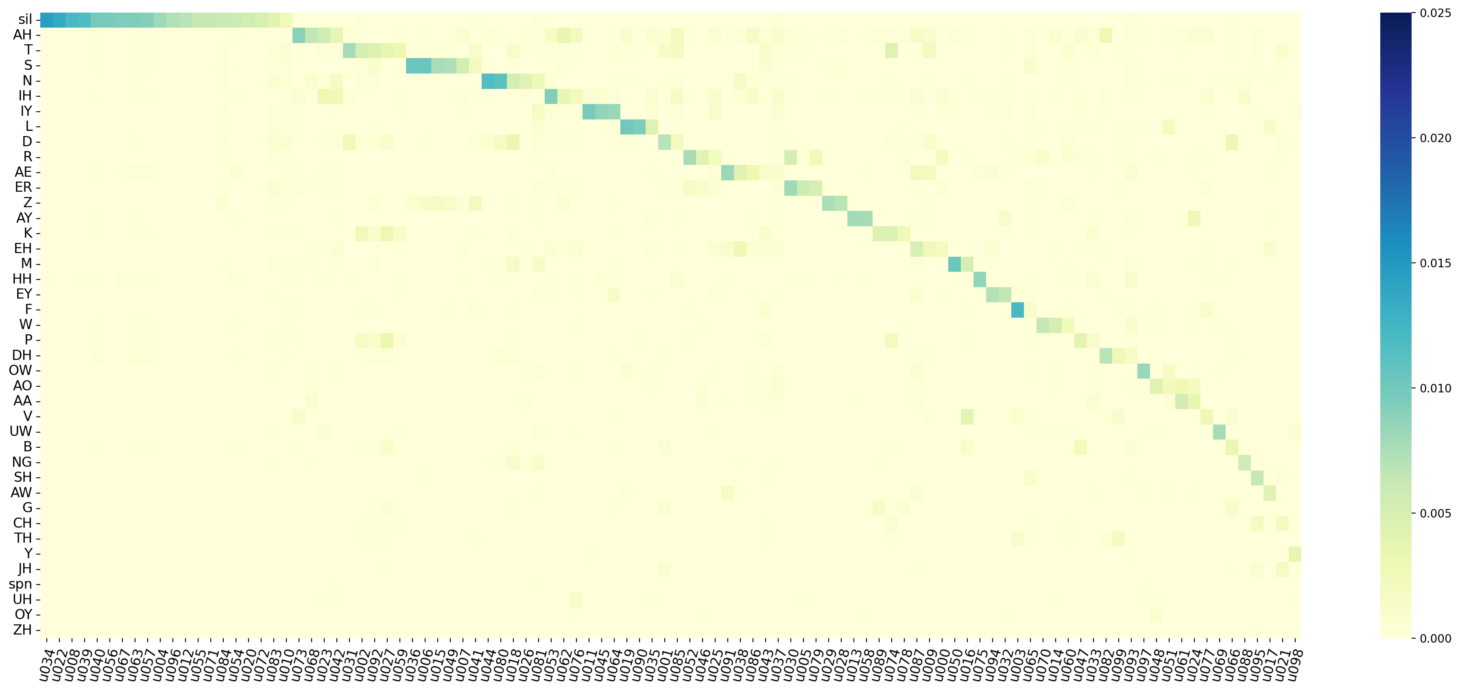
\includegraphics[width=1\linewidth]{figures/joint_sortby_prphn-hub-100.png}
            \caption{HuBERT 模型、群數 = 100 之 \\ 
            離散單元與音位標註的共同機率分佈圖}
            \label{fig:joint-byprob-hub100}
        \end{figure} 
    }
        圖中的縱軸表示各個音位,橫軸表示各個離散單元。在這張圖中,縱軸的音位是按照其邊際機率 \(p_y(i)\) 由高至低排序;橫軸的離散單元則是依據其對應的最高機率音位 \(y^\ast(j)\) 的縱軸排序位置進行排列。\footnote{如果兩個離散單元 \(j_1\) 和 \(j_2\) 對應到相同的音位 \(y^\ast = y^\ast(j_1) = y^\ast(j_2)\),則依照機率值 \(p_{yz}(y^\ast, j_1)\) 和 \(p_{yz}(y^\ast, j_2)\) 由高到低進行排序,對於多個離散單元的情況以此類推。} 這樣可以在熱圖上呈現出由左上至右下的對應關係。

        對於離散單元抽取的過程,
我們會希望模型的離散單元可以更加集中的

% 
\chapter{多個語音離散表徵與音位的關係}

\textcolor{red}{tokenization 的翻譯需要調整!}

\section{動機}

  如前一章所述,一個文字或音位往往對應到上百毫秒的語音訊號,然而單一離散單元所對應的聲音訊號為 10 或 20 毫秒,亦即同一段語音所對應的離散單元數目將比音位或文字多出許多。本章節從自然語言處理中獲取靈感,將分詞演算法(Tokenization)應用於離散單元序列上,並應用上一章節的分析方法檢驗將多個離散單元所組成之符記。探討分詞後,離散單元是否可以同時擁有無文字(Textless)\cite{lakhotia_generative_2021, lakhotia_generative_2021-1, noauthor_textless_2021} 的特性,且更接近音位的序列,成為更好的語音表徵。

\section{相關研究} 

  在無文字架構被提出後的約兩年後,藉分詞方法組合離散單元的研究逐步出現。最初提出「聲學片段(Acoustic Piece)」的是任氏(Ren)等人 \cite{ren_speech_2022}\citetag{1-22A4-Pretrain-ap}),該論文比對離散單元序列及對應的文字轉寫,從中觀察到許多相似的模式(Pattern),而且不限於單一語者。受此啟發,本論文首先將離散單元使用句子片段(SentencePiece) \cite{kudo_sentencepiece_2018} 分詞,獲得新的符記 --- 「聲學片段(Acoustic Piece)」,並用於語音辨識的預訓練上。

        不久,由吳氏(Wu)提出的 Wav2seq \cite{wu_wav2seq_2023}\citetag{2-22A5-wav2seq}論文中,考量文字與語音的序列長度差異,並基於離散單元和音位的關聯性,將離散單元視為字符(Character),嘗試將這些字符透過分詞方法組成「虛擬語言(Pseudo-language\footnote{偽語言對應之離散單元被視為「虛擬文字(Pseudo-text)」})」,來幫助語音到文字的模型。因為解碼器在實際應用時需要生成的序列多是文字的符記 --- 次詞單位(Subword Unit),因此該篇研究旨在讓模型在預訓練後可以快速適應下游任務。與前一篇呼應,「聲學片段」對語音預訓練的效果在\cite{10096788}\citetag{3-23A-coarser-grain}中被探討,此後聲學片段更被應用於縮短資料序列長度\cite{chang_exploration_2023}\citetag{4-23B-Exploration of Efficient End-to-End ASR using Discretized Input from Self-Supervised Learning} 、語音生成\cite{shen2024acoustic}\citetag{5-24A-speech-gen},或學習更穩健(Robust)的語音表徵\cite{chang2023r}\citetag{6-23B-rspin-acousticpiece}。

        近期,張氏(Chang)等人\cite{chang_exploring_2024}\citetag{7-23B-shinji-hsiuhsuan}將以分詞方法處理離散單元的流程(Pipeline)納入 ESPNet 套件 \cite{watanabe2018espnet} 中,並在語音辨識、語音翻譯等任務中獲得了超越以往的表現,進一步證明了這個方法的效果。

\section{分詞方法}

  在以文字為主體的自然語言處理中,文字文本除了以單詞(Word)或字元(Character)為處理單位,更常見的作法是透過分詞演算法(Tokenization)將文本分段,以「次詞單位(Subword Unit)」構成詞彙表來重新編碼文本,用於文字模型的訓練與推理。

        分詞方法的優點一般包含:

\begin{enumerate}
    \item 固定詞彙表大小,避免未登錄詞(Out-of-vocabulary,OOV)
    \item 縮短資料序列的長度,提升訓練和推論的效率。
    \item 分解單詞,捕捉更細緻的語意關係,模擬如英語中的字首(Prefix)、字尾(Suffix)等等具有特定意義的文字組合。
\end{enumerate}

\subsection{常見演算法}

  以下介紹幾種常見的分詞方法:

\paragraph{位元組對編碼(Byte Pair Encoding,BPE)}\hfill \break

  位元組對編碼 \cite{10.5555/177910.177914, sennrich_neural_2016} 是一種常用的分詞方法,最初來自資料壓縮技術 \cite{10.5555/177910.177914},後來被引入到自然語言處理領域,用以處理機器翻譯問題 \cite{sennrich_neural_2016} 。
該演算法從字元開始,根據詞彙表中各個次詞單位的頻率,反覆合併常見的字元成為新的次詞單位,直到達到預定的詞彙表大小。

\paragraph{單詞片段(WordPiece)}\hfill \break

  WordPiece \cite{wu2016google} 演算法由 Google 用以訓練機器翻譯系統,並在 BERT \cite{devlin_bert_2019} 模型中被使用而廣為人知。與 BPE 同樣是透過反覆合併的策略,但合併的依據改以機率模型取代出現頻率。

\paragraph{單一詞語言模型(Unigram Language Model)}\hfill \break

  單一詞語言模型 \cite{kudo2018subword} 是基於語言模型的分詞方法,以機率分佈選擇次詞單位,並以最大化輸入文本的機率來為文本分段。

\subsection{句子片段(SentencePiece)套件}

  SentencePiece \cite{kudo_sentencepiece_2018}
是由 Google 開發的分詞套件,實作了前述的 BPE 和單一詞演算法。其優勢在於可應用於不同語言,尤其用於處理中文、日文等不使用空格分隔單詞的語言文本時,此套件大大的簡化了前處理的流程。

\section{衡量方式}

  本章節沿用上一章節 LibriSpeech 資料集的 train-clean-100 訓練子集,以及相同的分析數據以進行比對。由於與上一章節的差異僅在分詞方法的引入,因此數據結果將多紀錄分詞前後序列長度的變化;其他操控變因包含分詞方法與詞表大小。考慮到語音訊號本身不如英語等文字,在書寫時就已經具備空格分隔單詞,因此以下分析結果皆採用 SentencePiece 套件中實作之單一詞演算法為分詞方法,並比較詞表大小 500、1000、8000、10000、20000 五種設定的結果差異。(空間不足時則僅呈現 500、1000、10000 三種設定的趨勢。)

\section{分析結果}\newcommand{\jefftablesep}{\vspace{0.5cm}}\renewcommand{\arraystretch}{0.7} % 調整行高

    以下數據中的「長度壓縮比率」係指透過分詞方法後,每一個句子的「單詞」數與原先離散單元的數量相比之比值。由於長度壓縮比率是針對離散單元分詞所得到,與標註無關,因此只在音位分析的表格上呈現。

\subsection{基於各自音位的分析}

  首先,為了比較不同詞表大小對於純度、相互資訊等數據的影響,先分別固定語音模型為 HuBERT 和 Wav2vec 2.0,在離散單元的分群數量為 50、100、200 三種設定下,觀察詞表大小造成的變化。由 HuBERT (表 \ref{tab:hubert-phn-results})和 Wav2vec 2.0(表 \ref{tab:w2v2-phn-results})的數據比較可觀察到,詞表大小上升除了使得音位純度提高以外,相互資訊也是隨之提高的,可以發現使用分詞方法並給予足夠大的詞表,對於找出語音中的資訊確實有所幫助。

        接著從另一個角度切入,比較同樣都是離散單元分群數為 200 的條件下,不同語音基石模型的分析數據。由表 \ref{tab:ch4-models-phn} 可以發現,HuBERT 模型在音位純度與相互資訊勝過其他模型,這個結論與上一章節是一致的。

        有趣的是,觀察長度壓縮比率可以發現,CPC 模型在分詞演算法的引入後,能夠使序列變得最短,但同時在音位純度與相互資訊上也有所犧牲;而 HuBERT 雖然在這些分析數據上高過其他三者,卻同時達成了比 Wav2vec 2.0 和 LogMel 更好的壓縮比率。因此綜合看來,或許這是為什麼目前使用語音離散單元進行研究時,HuBERT 模型仍然是領域內的首選。

                \input{tables/chapter4/chapter4-5.ztable1-1.tex}
\input{tables/chapter4/chapter4-5.ztable1-2.tex}
\input{tables/chapter4/chapter4-5.ztable1-3.tex}

\subsection{基於語音學分類的分析}

  最後觀察將語音標註換成語音學分類的結果,一樣可以從表 \ref{tab:hubert-pcls-results}、\ref{tab:w2v2-pcls-results} 和 \ref{tab:ch4-models-pcls} 觀察到與上一小節相同的趨勢。

                
        \begin{table}[!htbp]
            \centering
            \begin{subtable}[t]{\textwidth}
                \centering
                \begin{tabular}{|c|c|c|c|c|c|} \hline 
                        詞表大小  & 標註純度 & 分群純度 & 標註熵 & 離散單元熵 &     NMI   \\ \hline 
                       50 (未分詞)&   0.7466  &  0.1422 & 1.7530 &   3.8681 &  0.5742 \\ \hline 
                           500    &  0.7510  &  0.0345  & 1.7530 &  6.0282  &     0.5789  \\ \hline 
                          1000    &  0.7492  &  0.0225  & 1.7530 &  6.6594  &     0.5756  \\ \hline 
                          8000    &  0.7288  &  0.0116  & 1.7530 &  8.5192  &     0.5630  \\ \hline 
                         10000    &  0.7248  &  0.0110  & 1.7530 &  8.7207  &     0.5606  \\ \hline 
                         20000    &  0.7109  &  0.0089  & 1.7530 &  9.3527  &     0.5537  \\ \hline 
                \end{tabular}
\caption{群數 = 50}
                \label{tab:ch4-hubert-pcls-clu050}
            \end{subtable}        

            \jefftablesep        

            \begin{subtable}[t]{\textwidth}
                \centering
                \begin{tabular}{|c|c|c|c|c|c|} \hline 
                        詞表大小  & 標註純度 & 分群純度 & 標註熵 & 離散單元熵 &     NMI   \\ \hline 
 100 (未分詞)&              0.7804 &   0.0856 &         1.7530 &     4.5704 &  0.6148\\ \hline 
                           500    &  0.7787  &  0.0300  & 1.7530 &  6.0655  &     0.6178  \\ \hline 
                          1000    &  0.7751  &  0.0210  & 1.7530 &  6.7181  &     0.6176  \\ \hline 
                          8000    &  0.7507  &  0.0095  & 1.7530 &  8.5954  &     0.6030  \\ \hline 
                         10000    &  0.7468  &  0.0087  & 1.7530 &  8.7938  &     0.6008  \\ \hline 
                         20000    &  0.7347  &  0.0072  & 1.7530 &  9.4123  &     0.5943  \\ \hline 
                \end{tabular}
\caption{群數 = 100}
                \label{tab:ch4-hubert-pcls-clu100}
            \end{subtable}        

            \jefftablesep        

            \begin{subtable}[t]{\textwidth}
                \centering
                \begin{tabular}{|c|c|c|c|c|c|} \hline 
                        詞表大小  & 標註純度 & 分群純度 & 標註熵 & 離散單元熵 &     NMI   \\ \hline 
 200 (未分詞)&              0.8004 &   0.0464 &         1.7530 &     5.2681 &  0.6563\\ \hline 
                           500    &  0.7875  &  0.0269  & 1.7530 &  6.0986  &     0.6469  \\ \hline 
                          1000    &  0.7788  &  0.0170  & 1.7530 &  6.7786  &     0.6385  \\ \hline 
                          8000    &  0.7625  &  0.0071  & 1.7530 &  8.6544  &     0.6266  \\ \hline 
                         10000    &  0.7601  &  0.0064  & 1.7530 &  8.8535  &     0.6251  \\ \hline 
                         20000    &  0.7514  &  0.0051  & 1.7530 &  9.4737  &     0.6200   \\ \hline
                \end{tabular}
\caption{群數 = 200}
                \label{tab:ch4-hubert-pcls-clu200}
            \end{subtable}        

\caption{HuBERT 模型在不同詞表大小時的語音學類別分析數據}
            \label{tab:hubert-pcls-results}
        \end{table}

\begin{table}[!htbp]
    \centering
    \begin{subtable}[t]{\textwidth}
        \centering
        \begin{tabular}{|c|c|c|c|c|c|} \hline 
                詞表大小 & 標註純度 & 分群純度 & 標註熵 & 離散單元熵 &     NMI \\ \hline 
 50 (未分詞)&      0.6913 &   0.1570 &         1.7530 &     3.8215 &  0.4682\\ \hline 
                  500  &  0.7018 &    0.0339 &   1.7530 &   6.0328 &       0.4873  \\ \hline 
                 1000  &  0.7058 &    0.0273 &   1.7530 &   6.6250 &       0.4913  \\ \hline 
                 8000  &  0.7041 &    0.0158 &   1.7530 &   8.4954 &       0.4956  \\ \hline 
                10000  &  0.7033 &    0.0152 &   1.7530 &   8.6966 &       0.4963  \\ \hline 
                20000  &  0.6961 &    0.0128 &   1.7530 &   9.3471 &       0.4954  \\ \hline 
        \end{tabular}
\caption{群數 = 50}
        \label{tab:ch4-w2v2-pcls-clu050}
    \end{subtable}        

    \jefftablesep        

    \begin{subtable}[t]{\textwidth}
        \centering
        \begin{tabular}{|c|c|c|c|c|c|} \hline 
                詞表大小 & 標註純度 & 分群純度 & 標註熵 & 離散單元熵 &     NMI \\ \hline 
 100 (未分詞)&     0.7219 &   0.0889 &         1.7530 &     4.5284 &  0.5252 \\ \hline 
                  500  &  0.7142 &    0.0288 &   1.7530 &   6.0769 &       0.5297  \\ \hline 
                 1000  &  0.7132 &    0.0197 &   1.7530 &   6.7265 &       0.5294  \\ \hline 
                 8000  &  0.7173 &    0.0108 &   1.7530 &   8.5576 &       0.5352  \\ \hline 
                10000  &  0.7171 &    0.0105 &   1.7530 &   8.7602 &       0.5360  \\ \hline 
                20000  &  0.7149 &    0.0089 &   1.7530 &   9.4070 &       0.5379  \\ \hline 
        \end{tabular}
\caption{群數 = 100}
        \label{tab:ch4-w2v2-pcls-clu100}
    \end{subtable}        

    \jefftablesep        

    \begin{subtable}[t]{\textwidth}
        \centering
        \begin{tabular}{|c|c|c|c|c|c|} \hline 
                詞表大小 & 標註純度 & 分群純度 & 標註熵 & 離散單元熵 &     NMI \\ \hline 
  200 (未分詞)&     0.7490 &   0.0527 &         1.7530 &     5.2173 &  0.5671  \\ \hline 
                  500  &  0.7465 &    0.0310 &   1.7530 &   6.0756 &       0.5685  \\ \hline 
                 1000  &  0.7451 &    0.0199 &   1.7530 &   6.7483 &       0.5692  \\ \hline 
                 8000  &  0.7405 &    0.0071 &   1.7530 &   8.6065 &       0.5725  \\ \hline 
                10000  &  0.7399 &    0.0066 &   1.7530 &   8.8136 &       0.5729  \\ \hline 
                20000  &  0.7391 &    0.0055 &   1.7530 &   9.4561 &       0.5757   \\ \hline
        \end{tabular}
\caption{群數 = 200}
        \label{tab:ch4-w2v2-pcls-clu200}
    \end{subtable}        

\caption{Wav2vec 2.0 模型在不同詞表大小時的語音學類別分析數據}
    \label{tab:w2v2-pcls-results}
\end{table}


        \begin{table}[!htbp]
            \centering
            \begin{subtable}[t]{\textwidth}
                \centering
                \begin{tabular}{|c|c|c|c|c|c|} \hline 
                        詞表大小  & 標註純度 & 分群純度 & 標註熵 & 離散單元熵 &     NMI  \\ \hline 
  200 (未分詞)&         0.8004 &   0.0464 &         1.7530 &     5.2681 &  0.6563\\ \hline 
                            500 &  0.7875 &    0.0269 &   1.7530   & 6.0986 &    0.6469 \\ \hline %%   2.0934
                           1000 &  0.7788 &    0.0170 &   1.7530   & 6.7786 &    0.6385 \\ \hline %%   2.1156
                          10000 &  0.7601 &    0.0064 &   1.7530   & 8.8535 &    0.6251 \\ \hline %%   2.1826
                \end{tabular}
\caption{HuBERT}
                \label{tab:ch4-pcls-model-hubert}
            \end{subtable}        

            \jefftablesep        

            \begin{subtable}[t]{\textwidth}
                \centering
                \begin{tabular}{|c|c|c|c|c|c|} \hline 
                        詞表大小  & 標註純度 & 分群純度 & 標註熵 & 離散單元熵 &     NMI  \\ \hline 
  200 (未分詞)&         0.7490 &   0.0527 &         1.7530 &     5.2173 &  0.5671 \\ \hline 
                            500 &  0.7465 &    0.0310 &   1.7530   & 6.0756 &    0.5685 \\ \hline %%   1.7491
                           1000 &  0.7451 &    0.0199 &   1.7530   & 6.7483 &    0.5692 \\ \hline %%   1.7727
                          10000 &  0.7399 &    0.0066 &   1.7530   & 8.8136 &    0.5729 \\ \hline %%   1.8791
                \end{tabular}
\caption{Wav2vec 2.0}
                \label{tab:ch4-pcls-model-w2v2}
            \end{subtable}        

            
            \jefftablesep        

            \begin{subtable}[t]{\textwidth}
                \centering
                \begin{tabular}{|c|c|c|c|c|c|} \hline 
                        詞表大小  & 標註純度 & 分群純度 & 標註熵 & 離散單元熵 &     NMI  \\ \hline 
 200 (未分詞)&         0.7947 &   0.0644 &         1.7530 &     5.1885 &  0.6345 \\ \hline 
                            500 &  0.7925 &    0.0369 &   1.7530   & 6.0343 &    0.6368 \\ \hline %%   1.9677
                           1000 &  0.7882 &    0.0223 &   1.7530   & 6.7245 &    0.6349 \\ \hline %%   1.9818
                          10000 &  0.7609 &    0.0096 &   1.7530   & 8.8593 &    0.6175 \\ \hline %%   2.0277
                \end{tabular}
\caption{CPC}
                \label{tab:ch4-pcls-model-cpc}
            \end{subtable}        

            \jefftablesep        

            \begin{subtable}[t]{\textwidth}
                \centering
                \begin{tabular}{|c|c|c|c|c|c|} \hline 
                詞表大小 & 標註純度 & 分群純度 & 標註熵 & 離散單元熵 &     NMI \\ \hline 
  200 (未分詞)&         0.6107 &   0.0335 &         1.7530 &     5.2322 &  0.3652 \\ \hline 
                            500 &  0.6156 &    0.0247 &   1.7530   & 6.1035 &    0.3801 \\ \hline %%   1.0166
                           1000 &  0.6189 &    0.0137 &   1.7530   & 6.7602 &    0.3875 \\ \hline %%   1.0376
                          10000 &  0.6322 &    0.0096 &   1.7530   & 8.7579 &    0.4085 \\ \hline %%   1.1211
                \end{tabular}
\caption{LogMel}
                \label{tab:ch4-pcls-model-logmel}
            \end{subtable}        

\caption{固定離散單元群數皆為 200,不同基石模型的語音學類別分析數據}
            \label{tab:ch4-models-pcls}
        \end{table}
        


\section{本章總結}

  藉由分詞演算法的引入,我們可以發現在序列長度相對縮短的前提下,音位的純度卻也獲得了提升,足以證明分詞演算法的引入,可以幫助離散單元考量多於一個音框的語音資訊,建構於精細的音框之上,找出更接近人類解讀語音最小單位資訊。期望以此發現,可以使得語音語言模型建立時,模型在處理語音語料庫時,能夠以更接近文字的序列長度與資訊進行訓練,獲得更接近文字模型的效果。

% ! TEX root = ../../realeasythesis.tex  % jeffhere

\chapter{多個語音離散表徵與音位的關係}   \newcommand{\jefftablesep}{\vspace{0.5cm}}
\renewcommand{\arraystretch}{0.7}
\newcommand{\jcm}[1]{}


% \newcommand{\jefftablesep}{\vspace{0.5cm}}\renewcommand{\arraystretch}{0.7} % 調整行高

\section{動機} %%%

  如第三章所述,一個文字或音位往往對應到上百毫秒的語音訊號,然而單一離散單元所對應的聲音訊號為 10 或 20 毫秒,亦即同一段語音所對應的離散單元數目將比音位或文字多出許多。本章節從自然語言處理中獲取靈感,將文字處理中的分詞演算法(Tokenization)應用於離散單元序列上,使得離散單元重新組合成次詞單位(Subword Units),稱之為「聲學片段(Acoustic Piece)」,以這些由多個離散單元組成的符記(Token)\footnote{指資料序列中的離散基本單位。}作為新的基本單位重新編碼語音訊號,取代原先的離散單元。為了分析聲學片段是否更接近音位的序列,在此將續用上一章節的分析方法,比對並檢驗引入次詞單位是否有機會得到更好的語音表徵,進而有機會用於無文字(Textless)架構\cite{lakhotia_generative_2021, lakhotia_generative_2021-1, noauthor_textless_2021}中。

\section{相關研究} 

  在無文字架構被提出後的約兩年後,藉助次詞單位組合離散單元的研究逐步出現。任氏(Ren)等人 \cite{ren_speech_2022}\citetag{1-22A4-Pretrain-ap})最先提出聲學片段的概念,該論文比對離散單元序列及對應的文字轉寫,從中觀察到許多相似的規律重複出現,而且不限於單一語者。受此啟發,本論文首先將離散單元,透過文字處理中常用以獲得次詞單位的「句片段(SentencePiece) \cite{kudo_sentencepiece_2018} 套件獲得新的符記 --- 「聲學片段」,並用於語音辨識的預訓練上。

        不久,由吳氏(Wu)提出的 Wav2seq \cite{wu_wav2seq_2023}\citetag{2-22A5-wav2seq}論文中,考量文字與語音的序列長度差異,並基於離散單元和音位的關聯性,將離散單元視為字符(Character),嘗試將這些字符透過次詞單位組成「虛擬語言(Pseudo-language\footnote{偽語言對應之離散單元被視為「虛擬文字(Pseudo-text)」})」,來幫助語音到文字的模型。在實際應用中,因為解碼器生成的目標文字序列亦是由次詞單位組成,因此該篇研究旨在讓模型在預訓練後可以快速適應下游任務。與前一篇呼應,聲學片段對語音預訓練的效果在\cite{10096788}\citetag{3-23A-coarser-grain}中被探討,此後聲學片段更被應用於縮短資料序列長度\cite{chang_exploration_2023}\citetag{4-23B-Exploration of Efficient End-to-End ASR using Discretized Input from Self-Supervised Learning} 、語音生成\cite{shen2024acoustic}\citetag{5-24A-speech-gen},或學習更穩健(Robust)的語音表徵\cite{chang2023r}\citetag{6-23B-rspin-acousticpiece}。

        近期,張氏(Chang)等人\cite{chang_exploring_2024}\citetag{7-23B-shinji-hsiuhsuan}將以分詞方法處理離散單元的流程(Pipeline)納入 ESPNet 套件 \cite{watanabe2018espnet} 中,並在語音辨識、語音翻譯等任務中獲得了超越以往的表現,進一步證明了這個方法的效果。

\section{文字處理中的分詞演算法}

  在以文字為主體的自然語言處理中,文字文本除了以單詞(Word)或字元(Character)為處理單位,更常見的作法是透過分詞演算法(Tokenization)將文本分段,以「次詞單位」構成詞彙表來重新編碼文本,用於文字模型的訓練與推理。

        使用次詞單位的優點包含:

\begin{enumerate}
    \item 固定詞彙表大小,避免未登錄詞(Out-of-vocabulary,OOV)。
    \item 縮短資料序列的長度,提升訓練和推論的效率。
    \item 分解單詞,捕捉更細緻的語意關係,模擬如英語中的字首(Prefix)、字尾(Suffix)等等具有特定意義的文字組合。
\end{enumerate}

\subsection{常見演算法}

  以下介紹幾種常見的分詞方法:

\paragraph{位元組對編碼(Byte Pair Encoding,BPE)} \hfill \break
%
  位元組對編碼 \cite{10.5555/177910.177914, sennrich_neural_2016} 是一種常用的分詞方法,最初來自資料壓縮技術 \cite{10.5555/177910.177914},後來被引入到自然語言處理領域,用以處理機器翻譯問題 \cite{sennrich_neural_2016} 。
該演算法從字元開始,根據詞彙表中各個次詞單位的頻率,反覆合併常見的字元成為新的次詞單位,直到達到預定的詞彙表大小。

\paragraph{單詞片段(WordPiece)} \hfill \break
%
  WordPiece \cite{wu2016google} 演算法由 Google 用以訓練機器翻譯系統,並在 BERT \cite{devlin_bert_2019} 模型中被使用而廣為人知。與位元組對編碼相似,同樣是透過反覆合併的策略,但合併的依據改以機率模型取代出現頻率。

\paragraph{單一詞語言模型(Unigram Language Model)} \hfill \break
%
  單一詞語言模型 \cite{kudo2018subword} 是基於語言模型的分詞方法,以機率分佈選擇次詞單位,並以最大化輸入文本的機率來為文本分段。

\subsection{「句片段(SentencePiece)」套件}

  「句片段(SentencePiece) \cite{kudo_sentencepiece_2018}
」是由 Google 開發的分詞套件,實作了前述的位元組對編碼和單一詞演算法。其優勢在於可應用於不同語言,尤其用於處理中文、日文等不使用空格分隔單詞的語言文本時,此套件大大的簡化了前處理的流程。
        考慮到語音訊號本身不如英語等文字,在書寫時就已經具備空格分隔單詞,因此本章節的所有次詞單位皆以句片段套件中的單一詞演算法取得。

\section{分析方式}

  本章節沿用上一章節 LibriSpeech 資料集的 train-clean-100 訓練子集,以單一詞演算法取得次詞單位,並嘗試 500、1000、8000、10000、20000 五種符記種數,對每一種語音表徵和 K-平均模型的分群數,各自取得五種聲學片段文本。

        比照第三章的分析方式,本章除了整體的純度與相互資訊數據外,亦同樣從聲學片段與音位的角度分別探討,藉由調整次詞單位的種類數量,探討引入次詞單位並改變符記數量,將如何影響這些符記序列與音位標註間的相關性。然而,為了避免結果呈現過於複雜,細部分析時將著重比對 500 和 1000 種次詞單位的結果變化。

        由於本章節探討重點為次詞單位種數變化的影響,延續第三章的發現,後續分析將以表現最好的 HuBERT 離散表徵為主。在需要比較離散單元分群數影響時,我們將比對分群數為 50 與 100 時的差異,否則為避免數據過於複雜,離散單元的分群數預設為 50 進行細部探討。

\section{分析結果} 

  承繼上一個章節的分析方法,我們先將純度等數據與條件機率熱圖 $p_{y|z}(i | j)$ \footnote{由於共同機率分佈熱圖 $p_{yz}$ 的數值對於觀察符記對應到音位的關係較不明顯,因此仿照 SpeechTokenizer \cite{zhang2024speechtokenizer}、DinoSR \cite{liu2024dinosr} 等論文使用 $p_{y|z}(i | j)$ 呈現。} 兩者互相對照,並以語音學排序呈現,觀察聲學片段與音位之間兩者的分佈關係。

\subsection{由聲學片段角度探討}
{
\subsubsection{聲學片段數量的影響}


{
\begin{table}[!htbp]
    \centering
    \begin{subtable}[t]{\textwidth}
        \centering
        \begin{tabular}{|c|c|c|c|c|c|} \hline 
                次詞單位種數& 音位純度 & 分群純度 & 音位熵 & 離散單元熵 &    PNMI \\ \hline 
離散單元& 0.5256& 0.3382& 3.3152& 3.8681& 0.4993\\ \hline 
                   500  &   0.5574   &  0.0829 &   3.3152  &  6.0282 & 0.5357 \\ \hline %%  1.7758       
                  1000  &   0.5744   &  0.0556 &   3.3152  &  6.6594 & 0.5466 \\ \hline %%  1.8120       
                  8000  &   0.5957   &  0.0257 &   3.3152  &  8.5192 & 0.5729 \\ \hline %%  1.8993       
                 10000  &   0.5955   &  0.0238 &   3.3152  &  8.7207 & 0.5750 \\ \hline %%  1.9063       
                 20000  &   0.5921   &  0.0182 &   3.3152  &  9.3527 & 0.5820 \\ \hline %%  1.9293       
        \end{tabular}
\caption{分群數 = 50}
        \label{tab:ch4-hubert-phn-clu050-}
    \end{subtable}        
    \jefftablesep        
    \begin{subtable}[t]{\textwidth}
        \centering
        \begin{tabular}{|c|c|c|c|c|c|} \hline 
                次詞單位種數& 音位純度 & 分群純度 & 音位熵 & 離散單元熵 &    PNMI \\ \hline 
離散單元& 0.6097& 0.2553& 3.3152& 4.5704& 0.5786\\ \hline 
                   500  &   0.6260   &  0.0972 &   3.3152  &  6.0655 & 0.5990 \\ \hline %%  1.9858       
                  1000  &   0.6372   &  0.0631 &   3.3152  &  6.7181 & 0.6089 \\ \hline %%  2.0186       
                  8000  &   0.6536   &  0.0237 &   3.3152  &  8.5954 & 0.6308 \\ \hline %%  2.0912       
                 10000  &   0.6527   &  0.0219 &   3.3152  &  8.7938 & 0.6324 \\ \hline %%  2.0965       
                 20000  &   0.6490   &  0.0173 &   3.3152  &  9.4123 & 0.6378 \\ \hline %%  2.1145       
        \end{tabular}
\caption{分群數 = 100}
        \label{tab:ch4-hubert-phn-clu100-}
    \end{subtable}        


\caption{HuBERT 模型在不同次詞單位種類數量時的純度分析數據}
    \label{tab:hubert-phn-results-}
\end{table}

}  % tables

{
    {
        \newcommand{\tempwidth}[0]{0.8\linewidth}
        \begin{figure}
             \centering
             \begin{subfigure}{\textwidth}
                 \centering
                 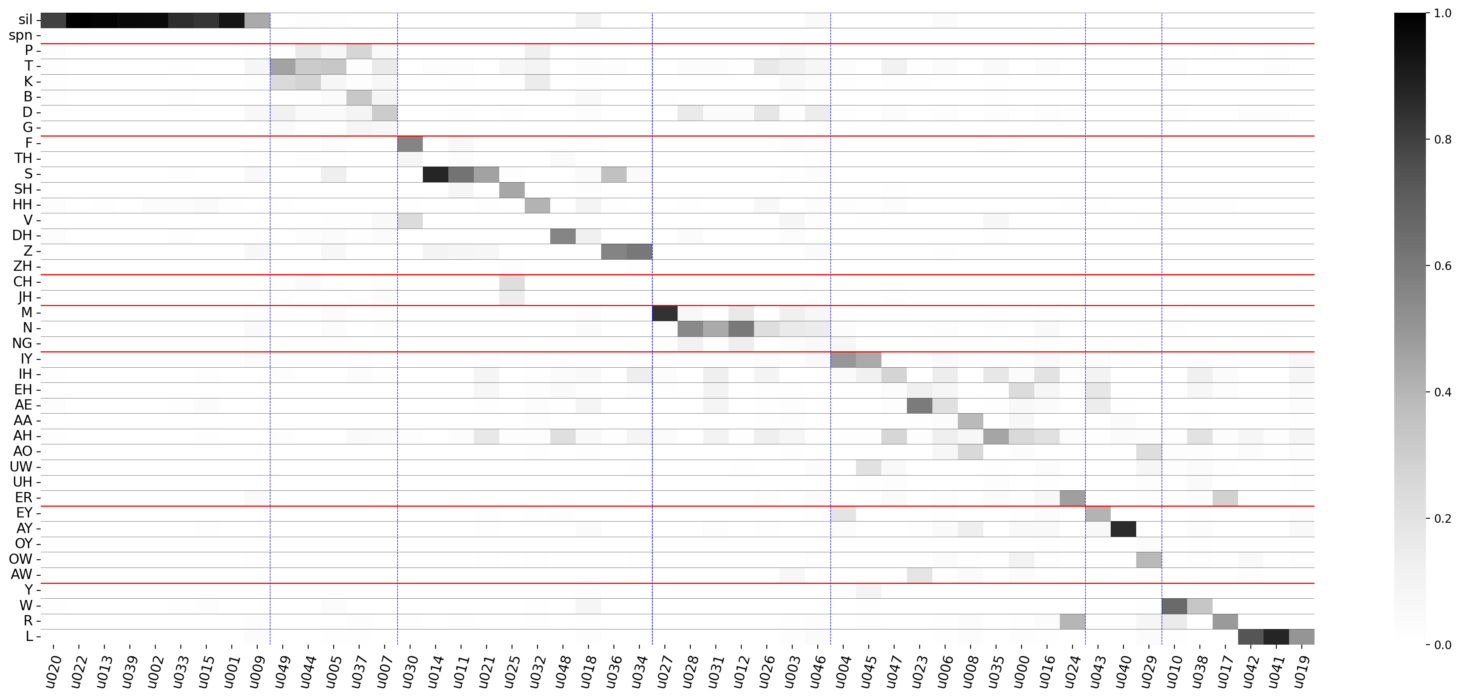
\includegraphics[width=\tempwidth]{figures/ch4figs/hub-u050-ap0000-givenunit-byphn.png}
                 \caption{離散單元}
                 \label{fig:hub-u050-ap0000-givenunit-byphn}
             \end{subfigure}
             \vfill
             \begin{subfigure}{\textwidth}
                 \centering
                 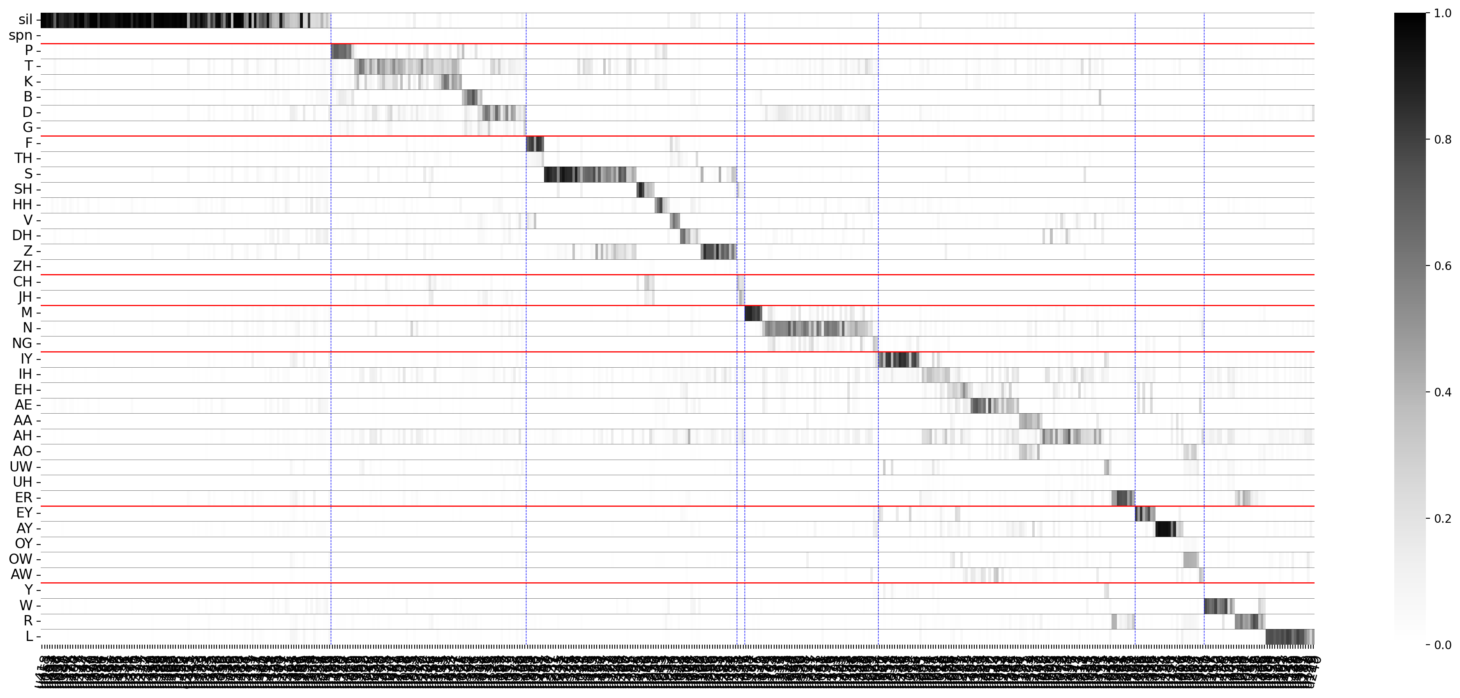
\includegraphics[width=\tempwidth]{figures/ch4figs/hub-u050-ap0500-givenunit-byphn.png}
                 \caption{500 種次詞單位}
                 \label{fig:hub-u050-ap0500-givenunit-byphn}
             \end{subfigure}
             \vfill
             \begin{subfigure}{\textwidth}
                 \centering
                 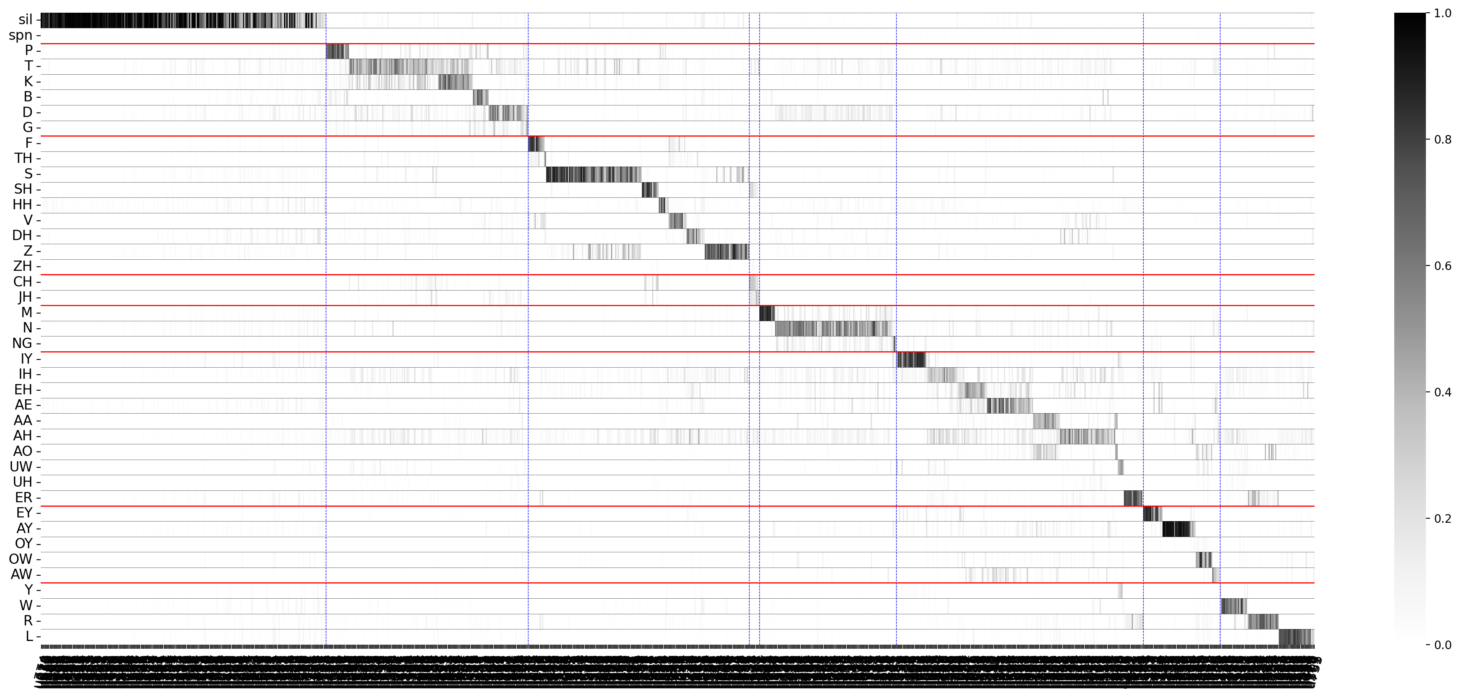
\includegraphics[width=\tempwidth]{figures/ch4figs/hub-u050-ap1000-givenunit-byphn.png}
                 \caption{1000 種次詞單位}
                 \label{fig:hub-u050-ap1000-givenunit-byphn}
             \end{subfigure}

             \caption{HuBERT 表徵在 K-平均演算法使用分群數 50 後,}
             比較不同次詞單位數量的條件機率分佈 $p_{y|z}(i | j)$ 熱圖
             \label{fig:hub-u050-comparisons}
        \end{figure}
    }
    {
        \newcommand{\tempwidth}[0]{0.8\linewidth}
        \begin{figure}
             \centering
             \begin{subfigure}{\textwidth}
                 \centering
                 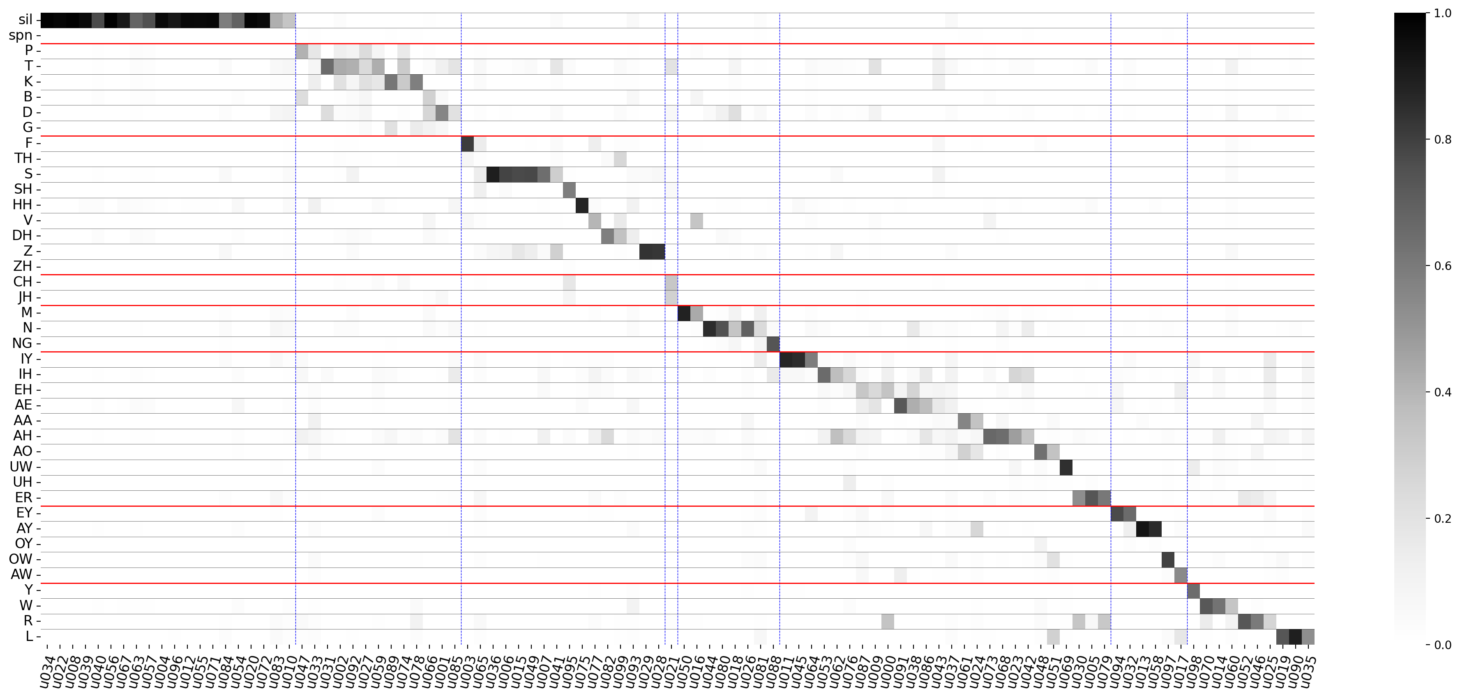
\includegraphics[width=\tempwidth]{figures/ch4figs/hub-u100-ap0000-givenunit-byphn.png}
                 \caption{離散單元}
                 \label{fig:hub-u100-ap0000-givenunit-byphn}
             \end{subfigure}
             \vfill
             \begin{subfigure}{\textwidth}
                 \centering
                 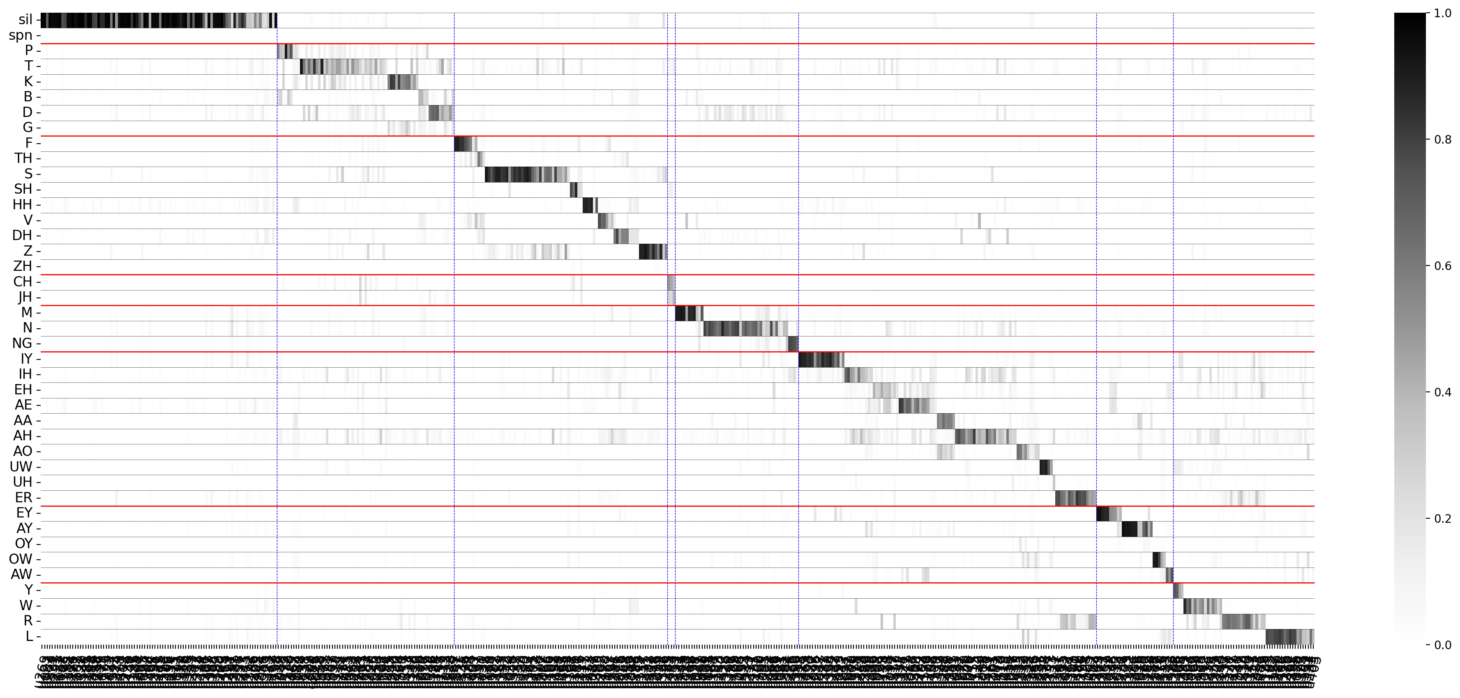
\includegraphics[width=\tempwidth]{figures/ch4figs/hub-u100-ap0500-givenunit-byphn.png}
                 \caption{500 種次詞單位}
                 \label{fig:hub-u100-ap0500-givenunit-byphn}
             \end{subfigure}
             \vfill
             \begin{subfigure}{\textwidth}
                 \centering
                 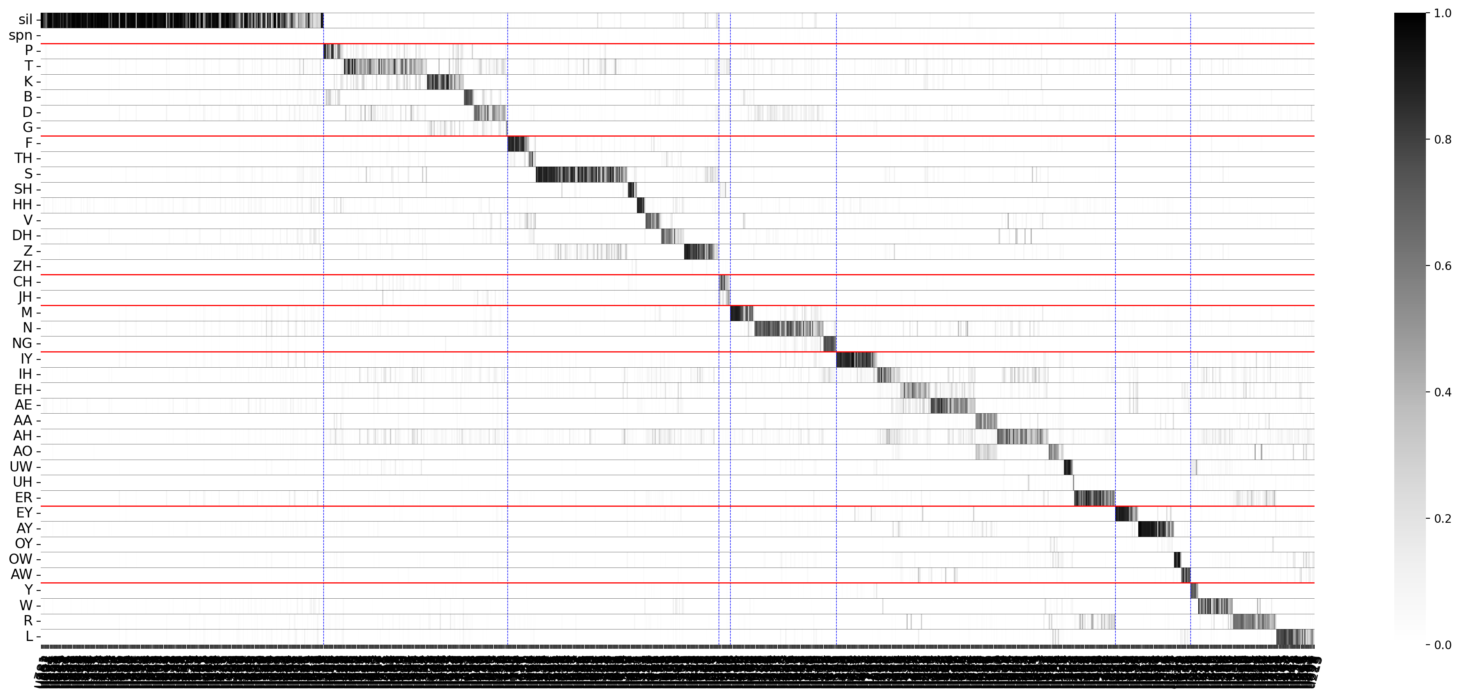
\includegraphics[width=\tempwidth]{figures/ch4figs/hub-u100-ap1000-givenunit-byphn.png}
                 \caption{1000 種次詞單位}
                 \label{fig:hub-u100-ap1000-givenunit-byphn}
             \end{subfigure}

             \caption{HuBERT 表徵在 K-平均演算法使用分群數 100 後,}
             比較不同次詞單位數量的條件機率分佈 $p_{y|z}(i | j)$ 熱圖
             \label{fig:hub-u100-comparisons}
        \end{figure}
    }
}

{
    {
        \newcommand{\tempwidth}[0]{0.7\linewidth}
        \begin{figure}
             \centering
             \begin{subfigure}{\textwidth}
                 \centering
                 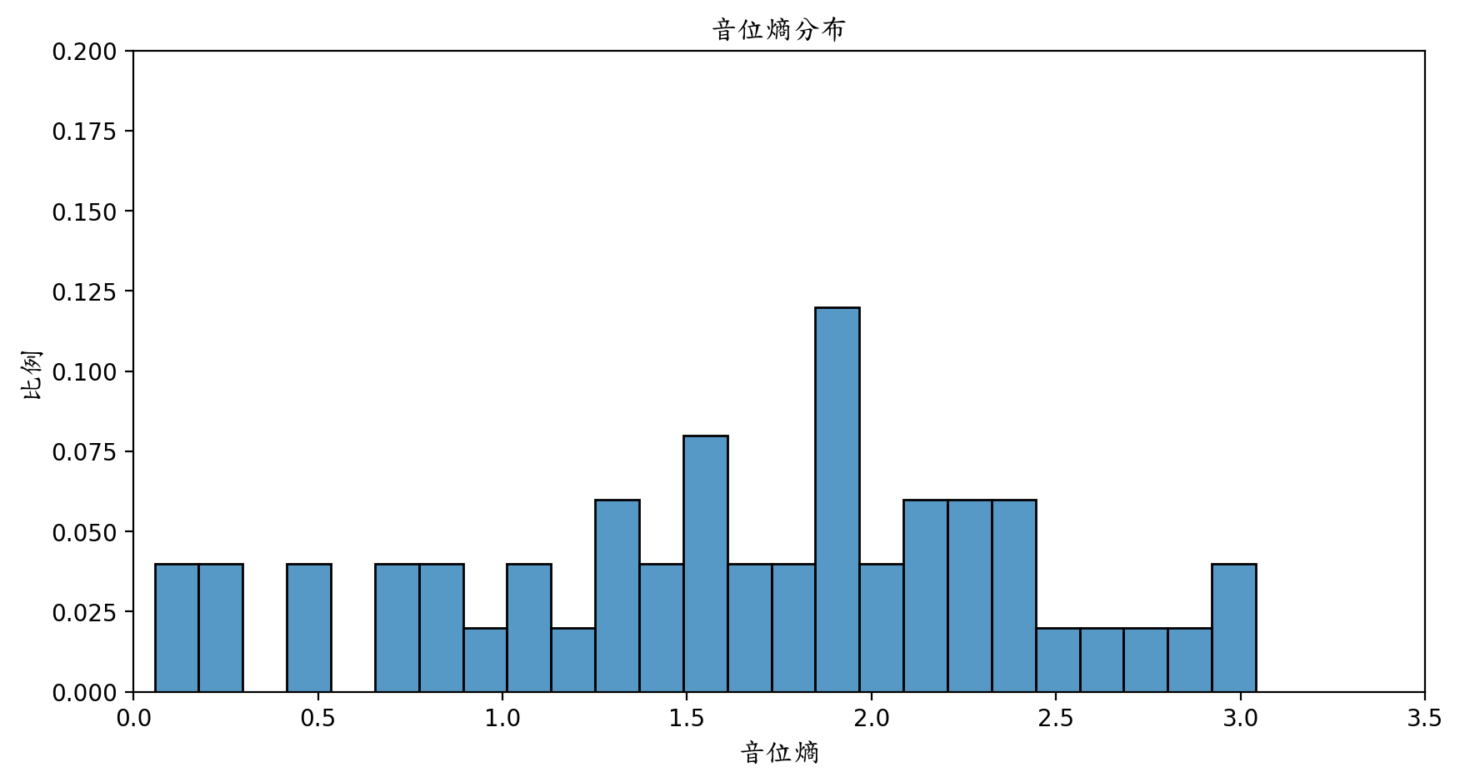
\includegraphics[width=\tempwidth]{figures/ch4figs/hub-u050-ap0000-phnent-hist.png}
                 \caption{離散單元}
                 \label{fig:hub-u050-ap0000-phnent-hist}
             \end{subfigure}
             \vfill
             \begin{subfigure}{\textwidth}
                 \centering
                 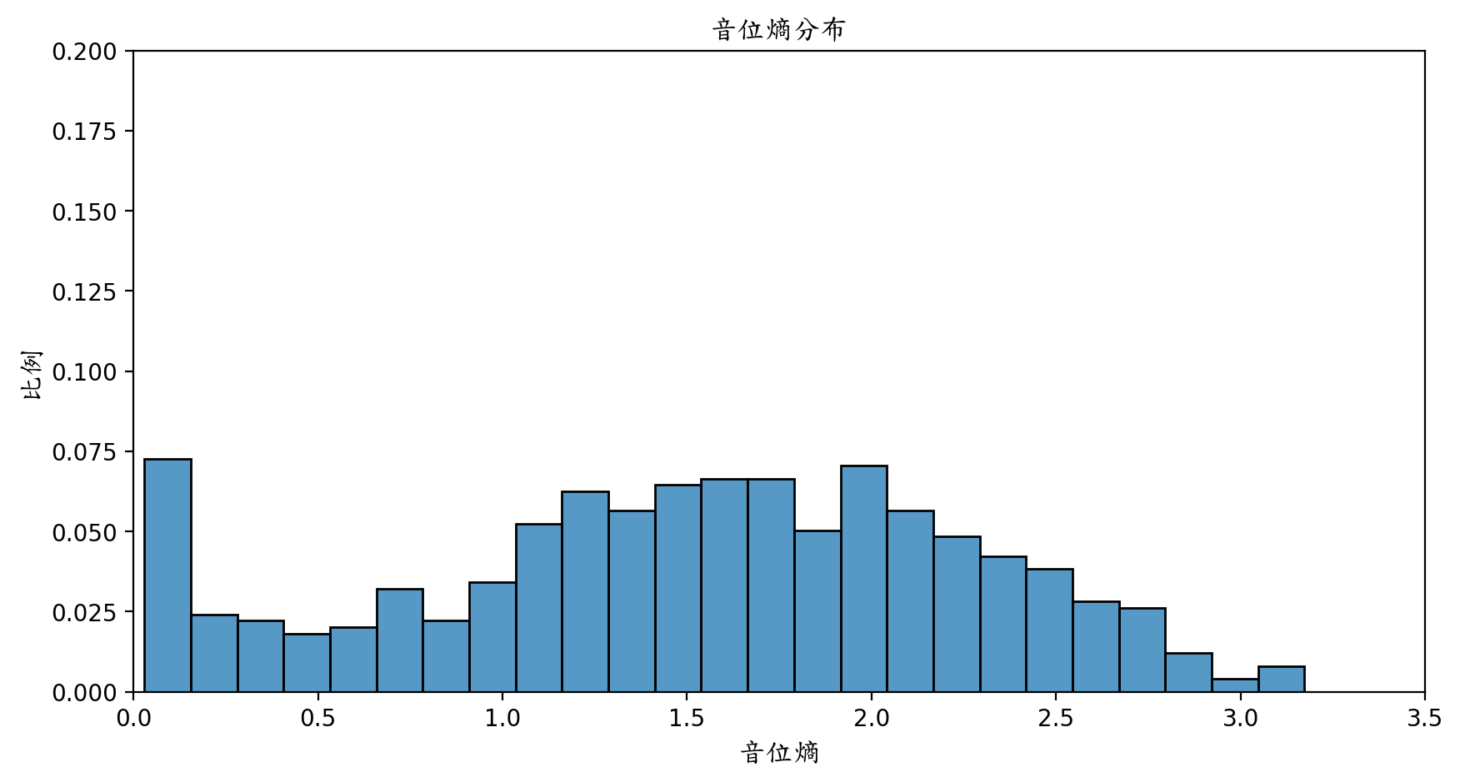
\includegraphics[width=\tempwidth]{figures/ch4figs/hub-u050-ap0500-phnent-hist.png}
                 \caption{500 種次詞單位}
                 \label{fig:hub-u050-ap0500-phnent-hist}
             \end{subfigure}
             \vfill
             \begin{subfigure}{\textwidth}
                 \centering
                 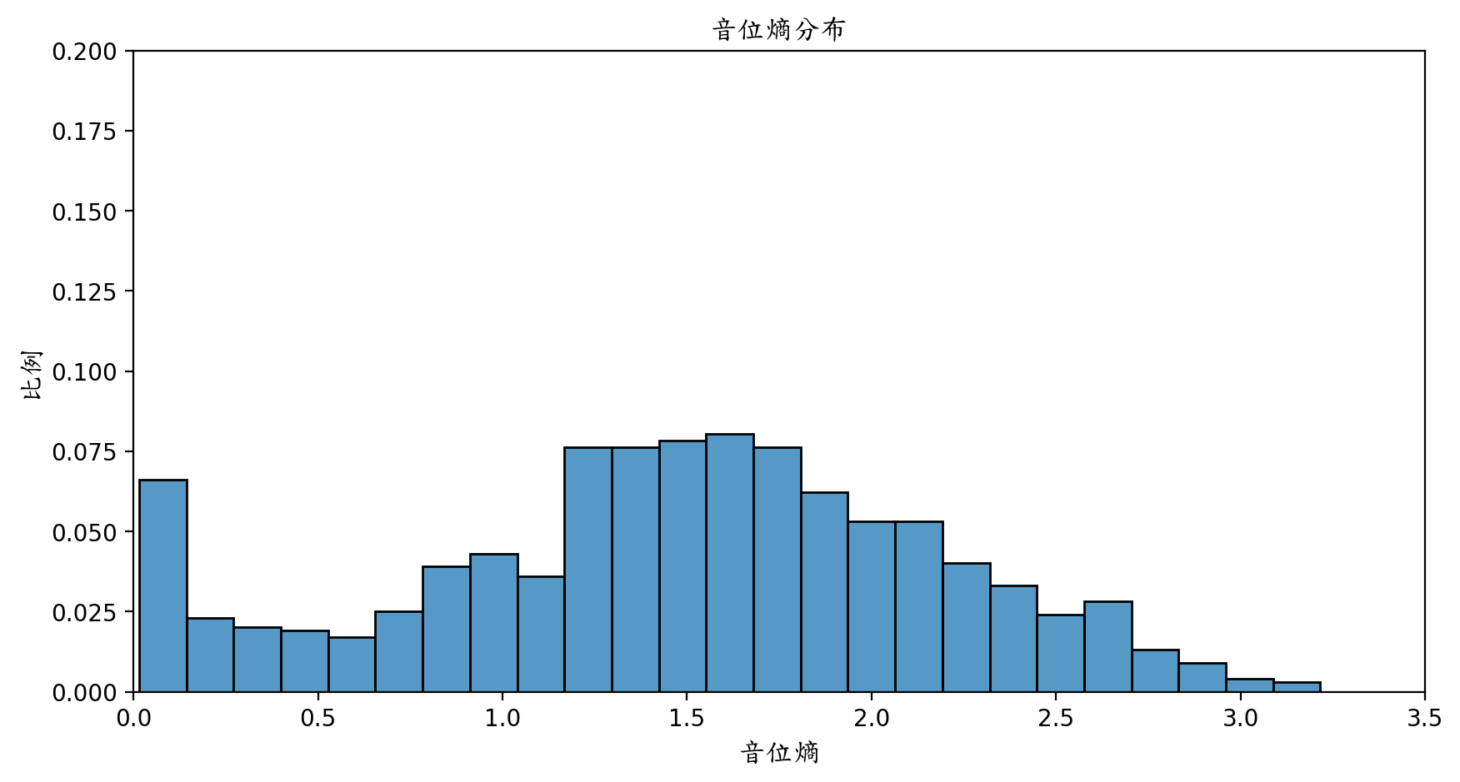
\includegraphics[width=\tempwidth]{figures/ch4figs/hub-u050-ap1000-phnent-hist.png}
                 \caption{1000 種次詞單位}
                 \label{fig:hub-u050-ap1000-phnent-hist}
             \end{subfigure}

             \caption{HuBERT 表徵在 K-平均演算法使用分群數 50 後,}
             比較不同次詞單位數量的音位條件熵 $H(y|z)$ 直方圖
             \label{fig:hub-u050-hist-comparisons}
        \end{figure}
    }
    {
        \newcommand{\tempwidth}[0]{0.7\linewidth}
        \begin{figure}
             \centering
             \begin{subfigure}{\textwidth}
                 \centering
                 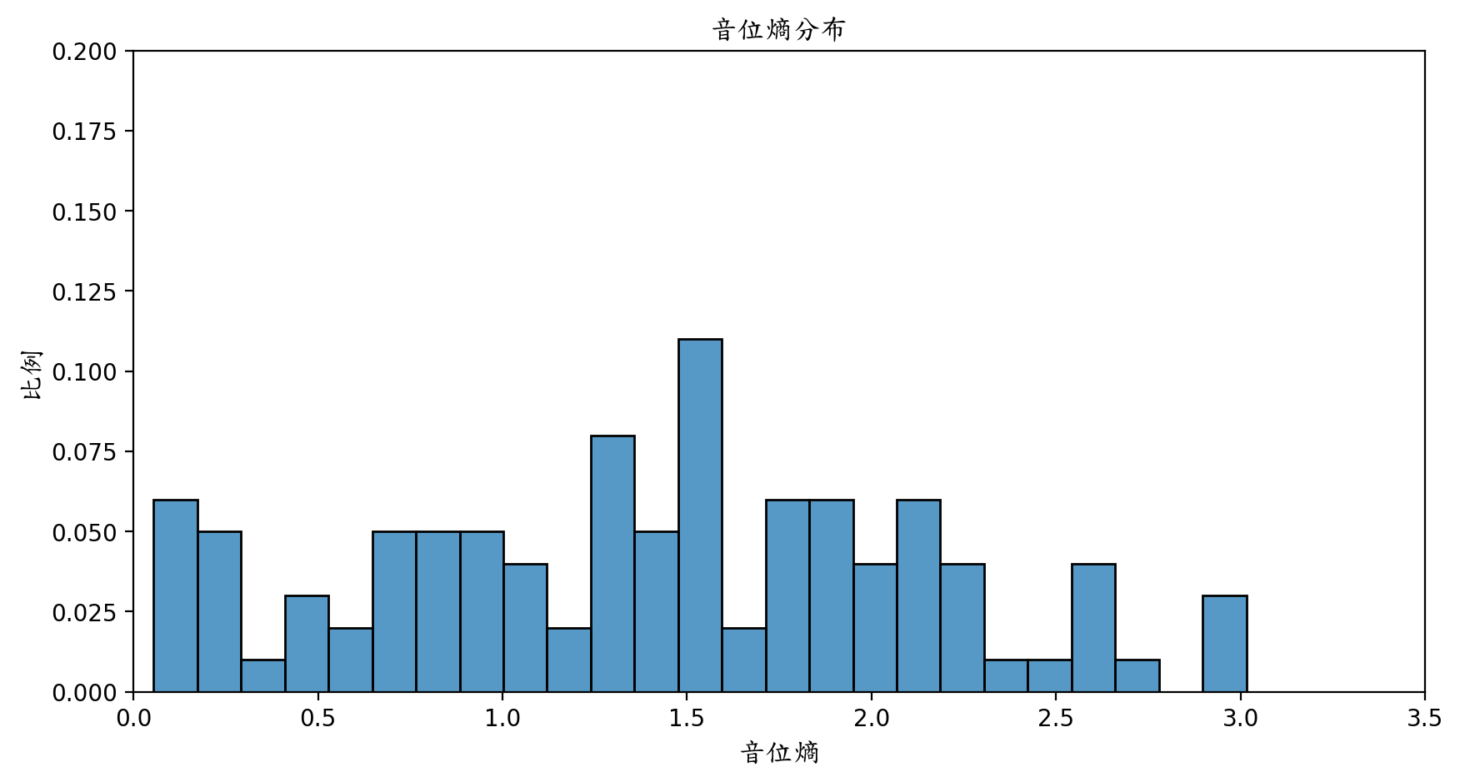
\includegraphics[width=\tempwidth]{figures/ch4figs/hub-u100-ap0000-phnent-hist.png}
                 \caption{離散單元}
                 \label{fig:hub-u100-ap0000-phnent-hist}
             \end{subfigure}
             \vfill
             \begin{subfigure}{\textwidth}
                 \centering
                 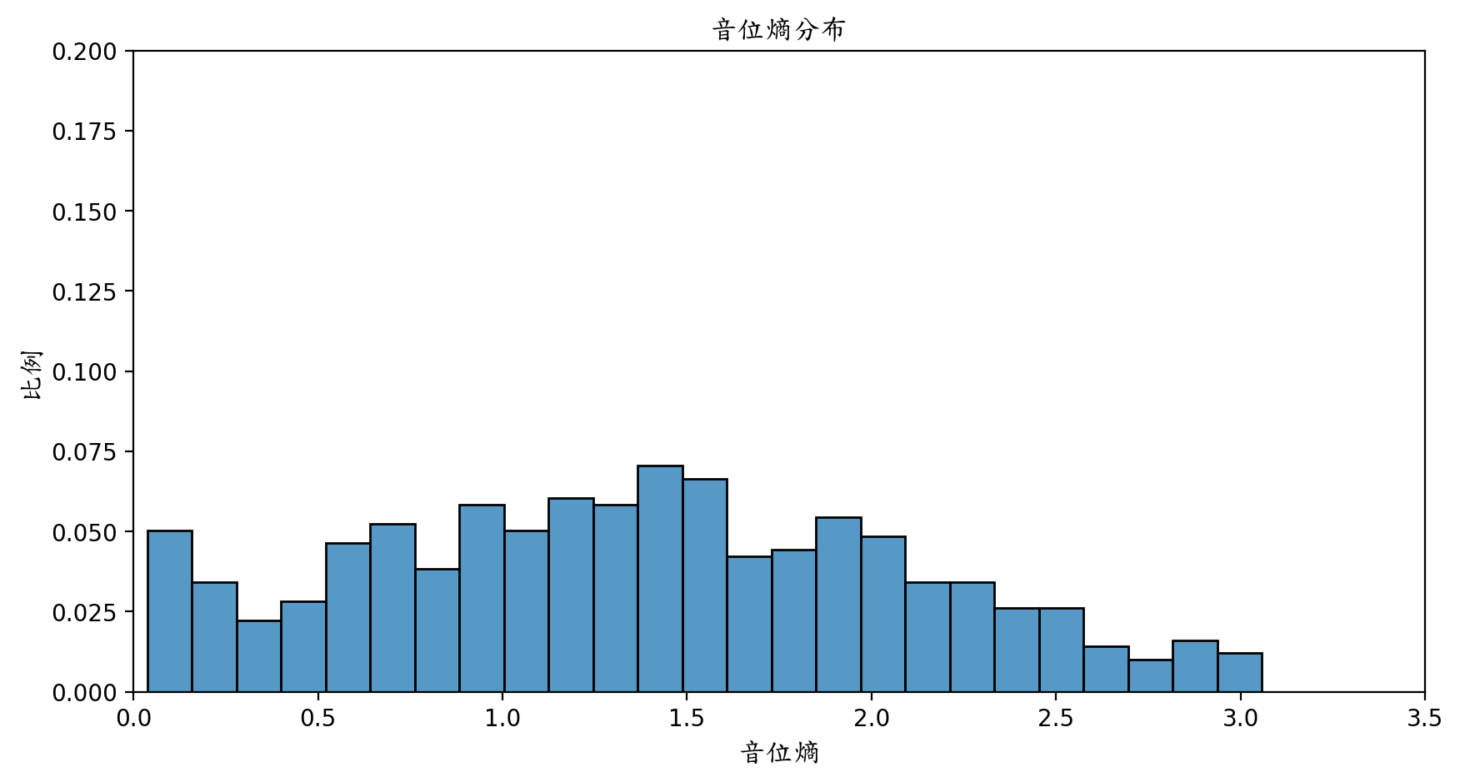
\includegraphics[width=\tempwidth]{figures/ch4figs/hub-u100-ap0500-phnent-hist.png}
                 \caption{500 種次詞單位}
                 \label{fig:hub-u100-ap0500-phnent-hist}
             \end{subfigure}
             \vfill
             \begin{subfigure}{\textwidth}
                 \centering
                 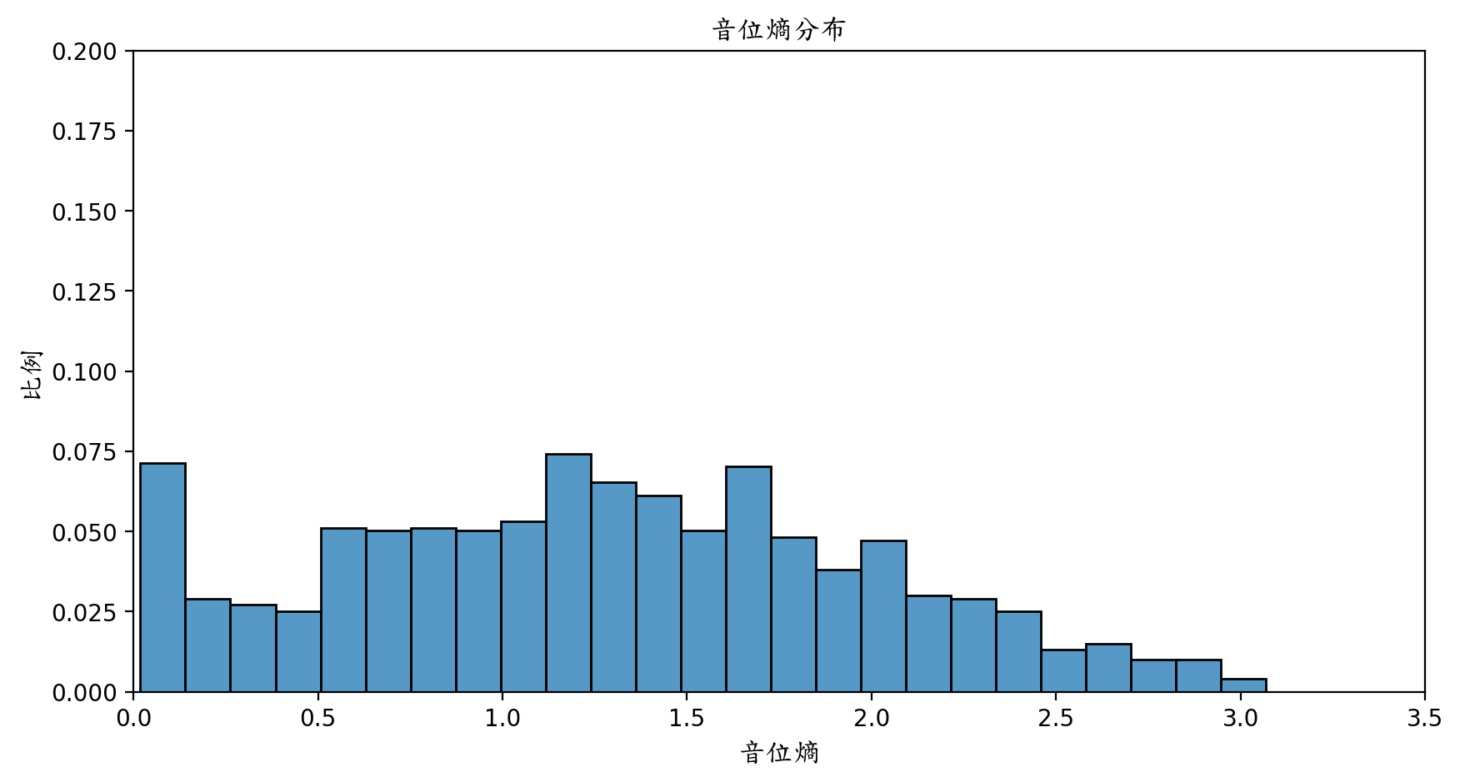
\includegraphics[width=\tempwidth]{figures/ch4figs/hub-u100-ap1000-phnent-hist.png}
                 \caption{1000 種次詞單位}
                 \label{fig:hub-u100-ap1000-phnent-hist}
             \end{subfigure}

             \caption{HuBERT 表徵在 K-平均演算法使用分群數 100 後,}
             比較不同次詞單位數量的音位條件熵 $H(y|z)$ 直方圖
             \label{fig:hub-u100-hist-comparisons}
        \end{figure}
    }
}


表 \ref{tab:hubert-phn-results-} 是 HuBERT 模型透過離散單元與不同次詞單位數量之聲學片段的純度與相互資訊數據。
首先,為了觀察聲學片段數量對於機率熱圖與純度數據的影響,圖 \ref{fig:hub-u050-comparisons} 與圖 \ref{fig:hub-u100-comparisons} 分別以
HuBERT 表徵、分群數為 50 和 100 的離散單元為基礎,比較原始離散單元、500 和 1000 種次詞單位三種設定下,不同聲學片段數量的條件機率熱圖。\jcm{它們分別是 HuBERT 模型配合分群數為 50 和 100 的離散單元模型,並將各自的離散單元使用單一詞演算法得到次詞單位數量為 500 和 1000 的聲學片段所得到的結果。}從中我們可以看出,當聲學片段數量上升時,熱圖可以觀察出許多更深的色塊,也就是有更多的聲學片段可以更集中的對應到特定音位。由此可見,有了更多樣的符記可以區別出更細節的發音差異,使整體的純度數值有所提升;然而,機率熱圖整體也變得更加破碎,因此歸類同樣音位的效果也相對變得較不明顯。

        為了確認各自聲學片段對應音位之集中狀況,我們可以考慮這些機率熱圖的條件音位熵 $H(y|z)$,以直方圖呈現來確認變化。透過觀察圖 \ref{fig:hub-u050-hist-comparisons} 與圖 \ref{fig:hub-u100-hist-comparisons} 的結果,可以確認相比第三章的離散單元,引入次詞單位確實能降低整體的條件音位熵,亦即新的符記各自能夠有更明確對應的音位,與我們從機率熱圖上所觀察到的趨勢符合。
        

        雖然改用聲學片段會使熱圖更加破碎而複雜,
% 難以觀察,
但
除純度與相互資訊的數值變化外,
觀察每個聲學片段對應之最高機率音位 $i^*(j)$ 以及它們的音位分類比例變化,
% 從符記代表性音位的比例變化,
也可以驗證「更多符記可以區別發音細節差異」這點。
再次觀察 HuBERT 在分群數 50 時的機率熱圖(圖 \ref{fig:hub-u050-comparisons}),圖 \ref{fig:hub-u050-comparisons} 中三章熱圖的藍色鉛直線
是
每個符記
在找出對應音位 $i^*(j)$ 後,按音位分類分區排序的結果。
因此,比較藍色鉛直線在橫軸上各區的比例變化,
可以知道
有多少比例的符記
能表示
特定類型的發音。
% 這些符記以多少的比例對應不同音位的發音特徵。
% \textcolor{red}{0000000000000000000000000000000000000000}
第三章結尾時提及過,在離散單元分群數為 50 時,由於符記數量較少,並沒有任何單元最能直接對應塞擦音音位。然而,當將這些離散單元以次詞單位進行重組後,不管在新符記種數為 500 或 1000 的機率熱圖上,都可以發現至少出現一個以上的符記得以對應到塞擦音。由此,我們驗證了引入次詞單位,對捕捉更細微的發音差異的確有所幫助。

\subsubsection{離散單元分群數對聲學片段表現的影響}

{
    {
        \begin{figure}
             \centering
             \begin{subfigure}{\textwidth}
                 \centering
                 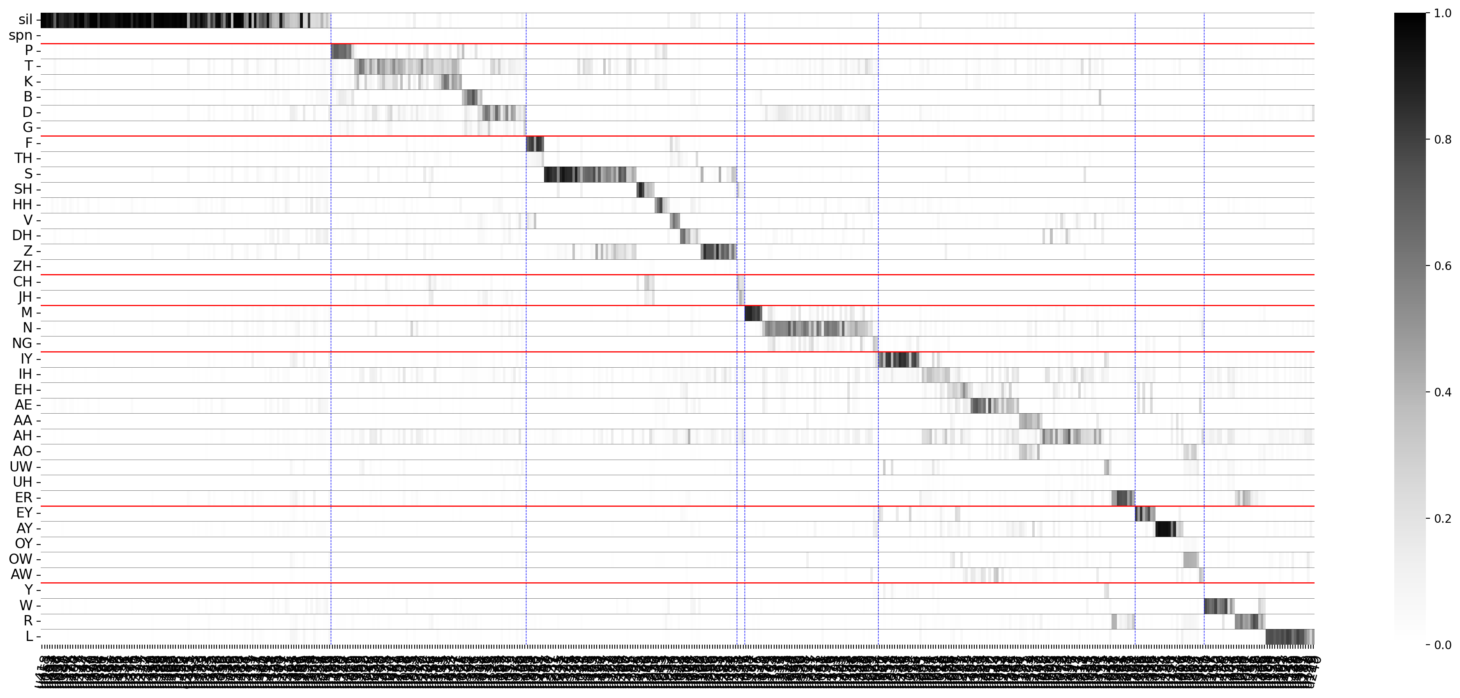
\includegraphics[width=1\linewidth]{figures/ch4figs/hub-u050-ap0500-givenunit-byphn.png}
                 \caption{分群數 50}
                 \label{fig:hub-u050-ap0500-givenunit-byphn--picked}
             \end{subfigure}
             \vfill
             \begin{subfigure}{\textwidth}
                 \centering
                 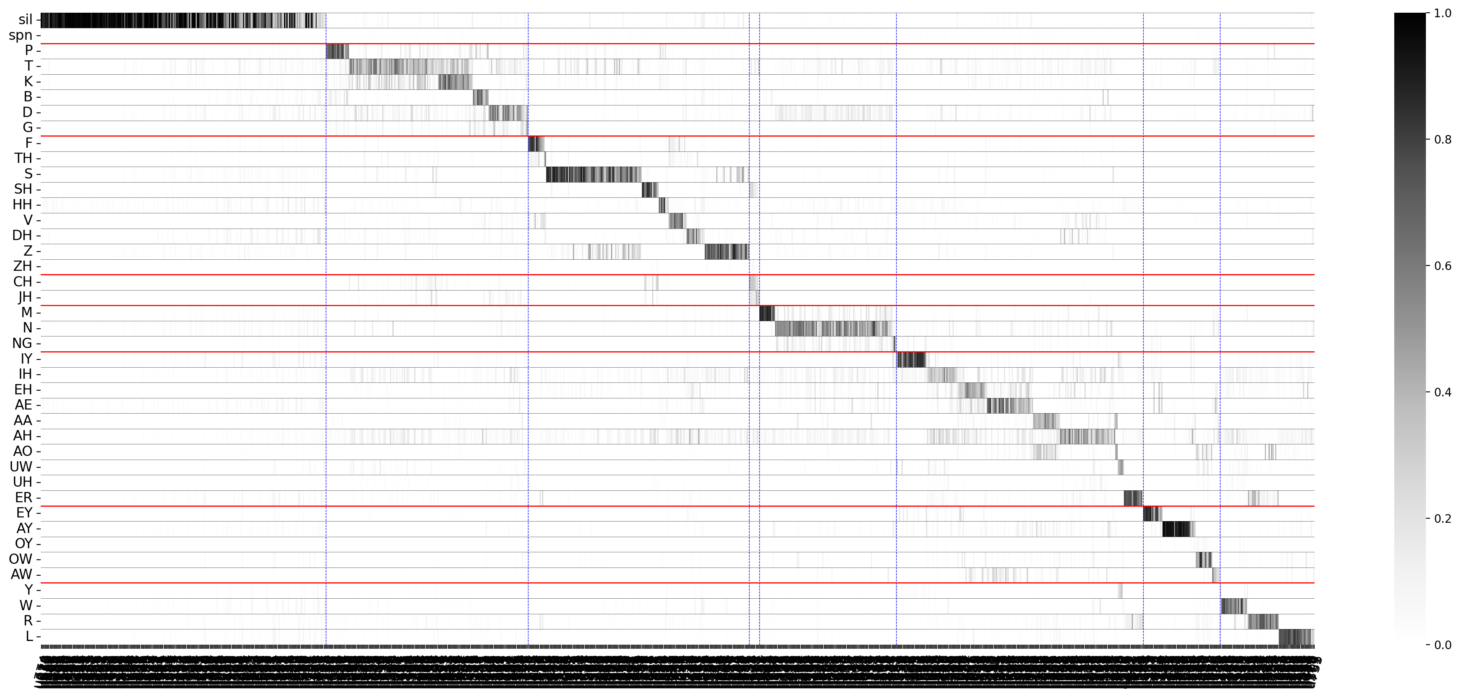
\includegraphics[width=1\linewidth]{figures/ch4figs/hub-u050-ap1000-givenunit-byphn.png}
                 \caption{分群數 100}
                 \label{fig:hub-u100-ap0500-givenunit-byphn--picked}
             \end{subfigure}
             \caption{比較同樣 500 種次詞單位的聲學片段模型,著重比較 HuBERT 表徵}
             在 K-平均演算法使用分群數 50 與 100 的條件機率熱圖 $p_{y|z}(i|j)$ 差異
             \label{fig:check-ap0500}
        \end{figure}
    }
}

  然而,儘管引入次詞單位一定程度上能幫助區別語音訊號中的細微發音差異,
% 若要更直接的改善對這件事進行改善,
在語音表徵進行離散化時,
K-平均演算法的分群數仍是決定
這些符記捕捉語音資訊
更關鍵的決定因素。
圖 \ref{fig:check-ap0500} 比較了同樣是 500 種次詞單位,K-平均演算法的離散表徵分群數選擇 50 和 100 的機率熱圖差異,不難發現分群數為 100 的機率熱圖能更加平均的對應到不同音位。然而,即便與音位的對應效果\jcm{對音位標註的歸類效果}最大取決於 K-平均的分群數,但分群演算法本身
相當消耗計算資源。因此
當遇到運算資源限制,致使 K-平均演算法的分群數難以設置得很大時,次詞單位的引入仍舊能提升整體表現。
        \jcm{藉由比較幾章機率熱圖的差異,我們可以確認這件事。 \jcm{補寫一下}}

        \jcm{
        
        我們這邊可以比較一下 50、100、50+100、50+500、100+500 的熱圖。從這邊可以驗證前面所說的:在基底分群數確定的情形之下,的確一開始分群數開得比較大,整體對語音規律的捕捉效果就會比較好,但藉由分群方法的引入,至少 50 分群數可以藉由符記數提升的機會,來重新編碼語音中的結構,也就是雖然不如 K-平均演算法那樣因為直接做用於語音表徵空間,那麼好區分出發音的差異,但藉由分詞演算法,仍然可以從捕捉語音中明顯重複的序列資訊\textcolor{red}{[這時候是不是要擺一下長度 & 常見 pattern 統計數據確認了?] } ,獲取語音序列中跟發音有關的特徵,進而模擬類似人類理解音位的過程。
        
        }
}

    {
        \newcommand{\tempwidth}[0]{0.8\linewidth}
        \begin{figure}
             \centering
             \begin{subfigure}{\textwidth}
                 \centering
                 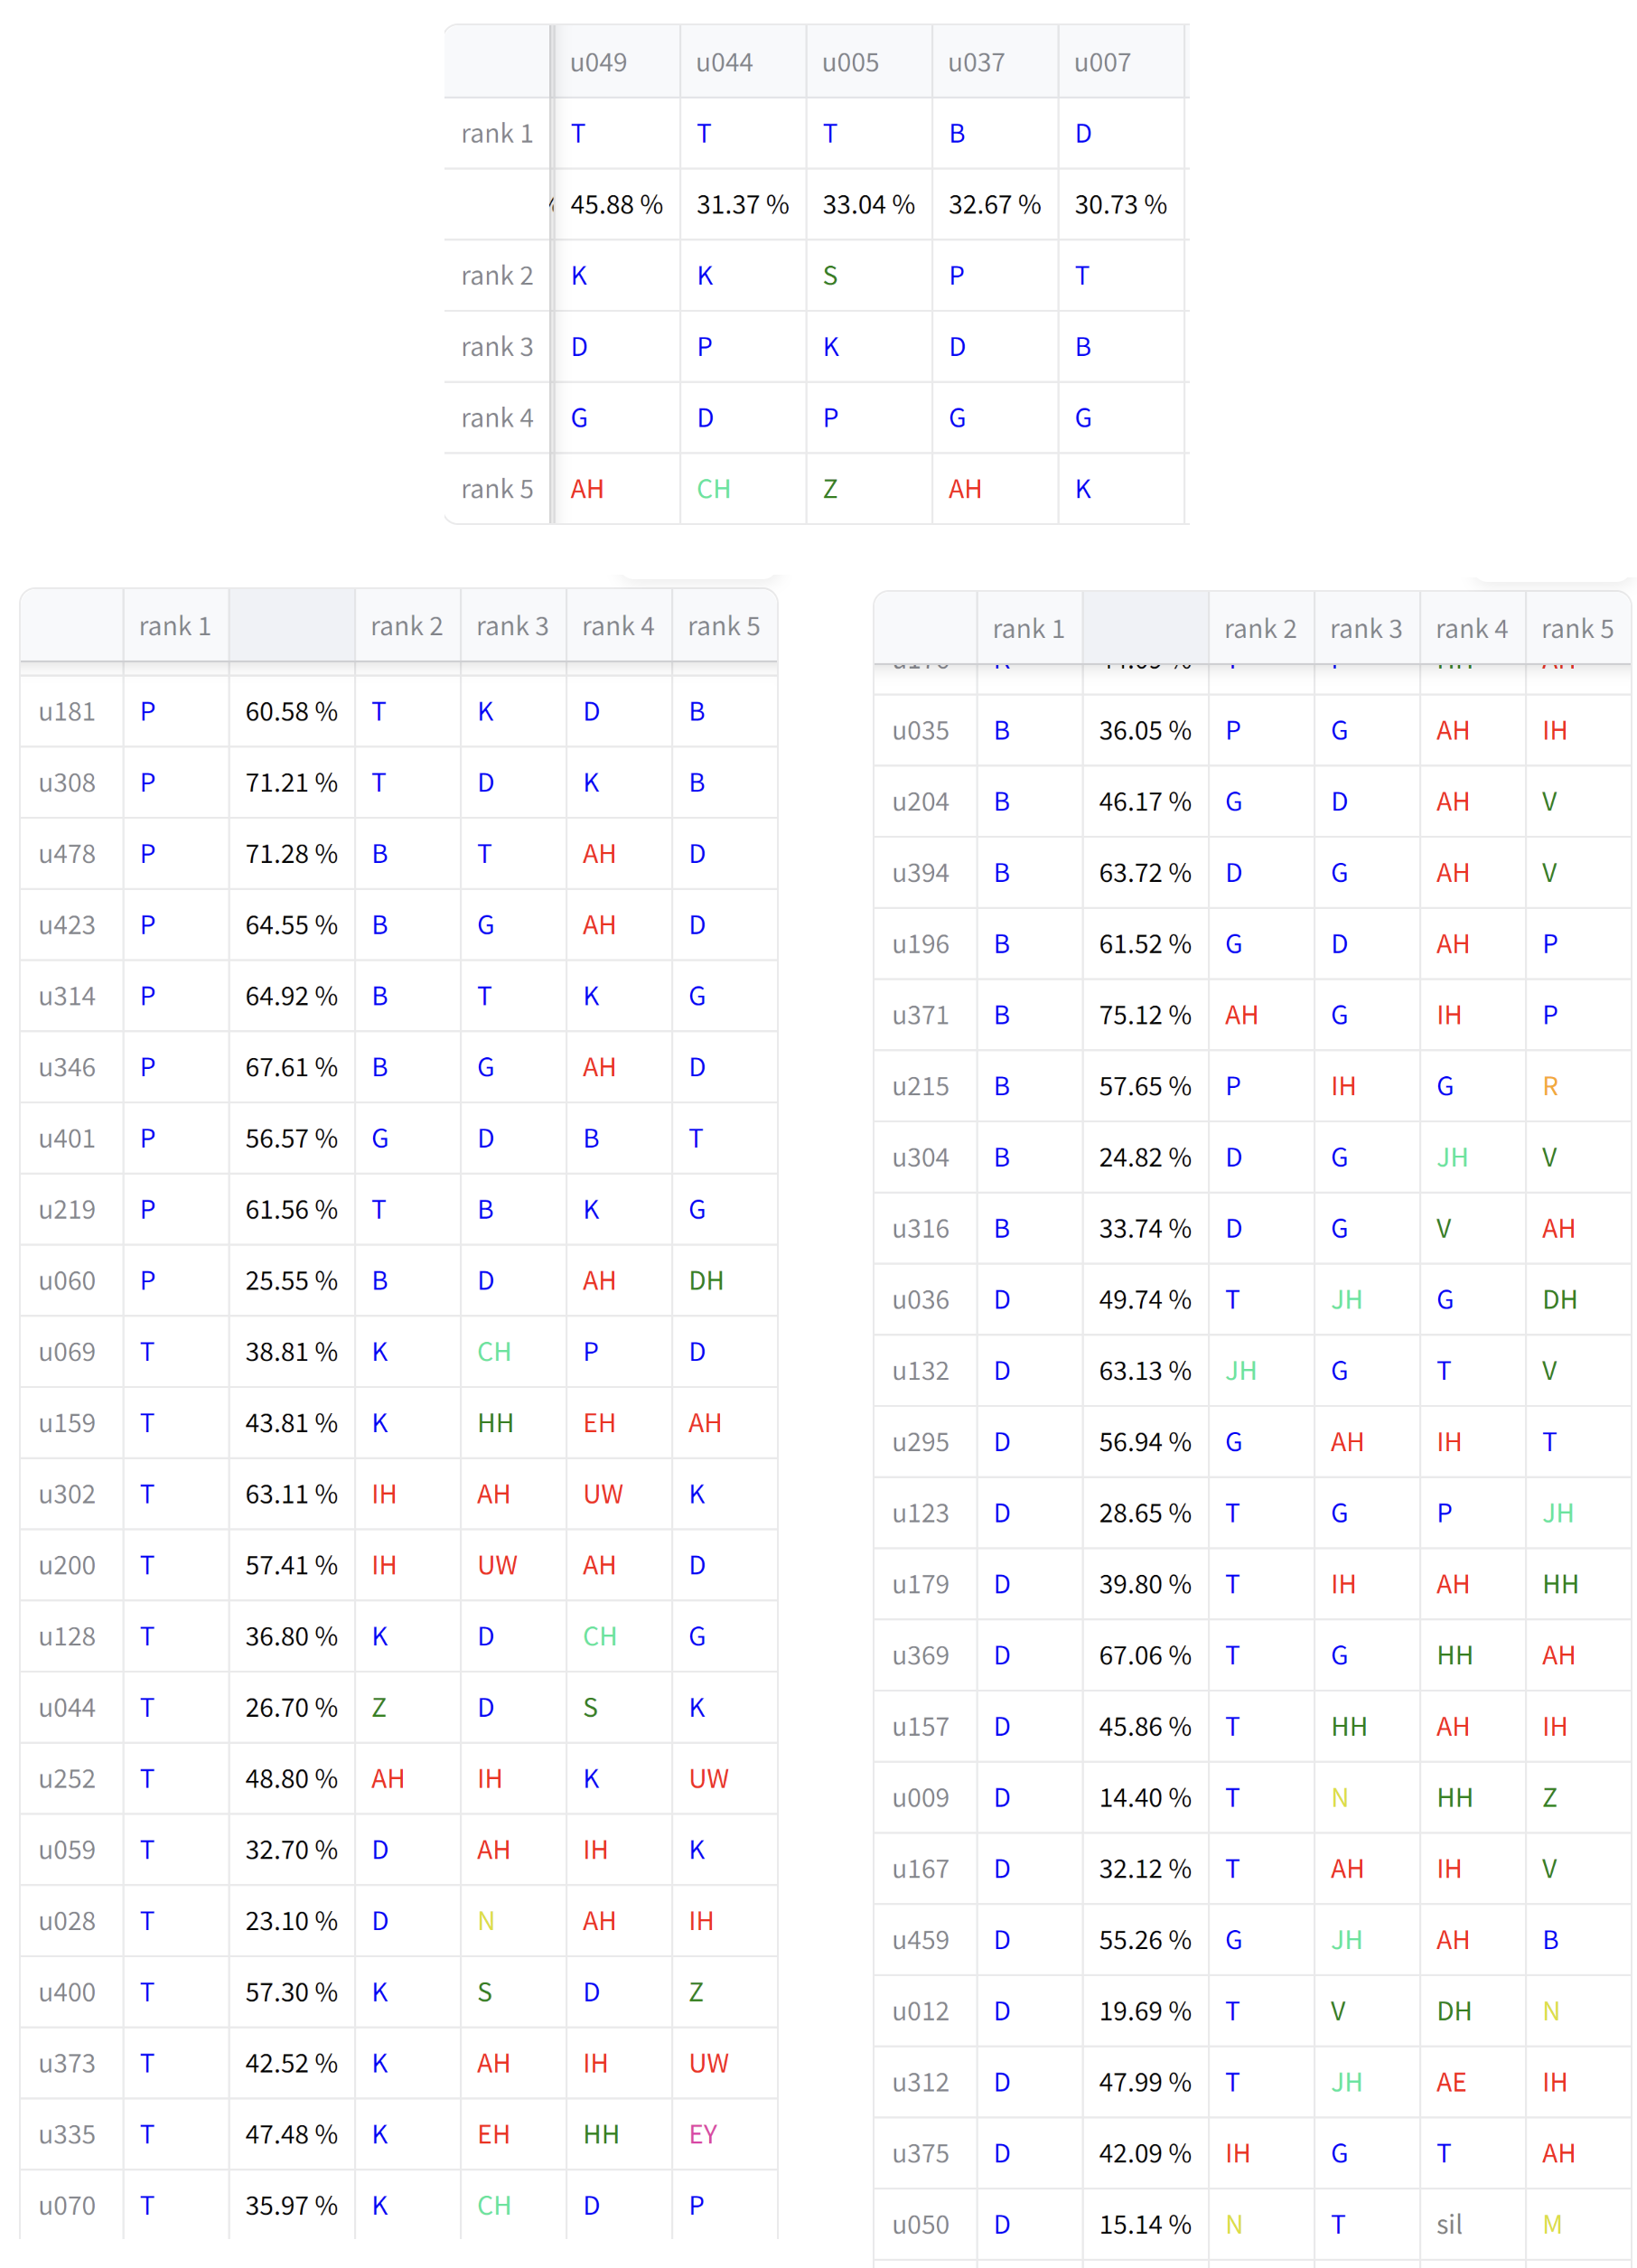
\includegraphics[width=\tempwidth]{figures/ch4figs/plo_phn.png}
                 \caption{塞音}
                 \label{fig:hub-u050-ap0500-ploobs}
             \end{subfigure}
             % \vfill
             % \begin{subfigure}{\textwidth}
             %     \centering
             %     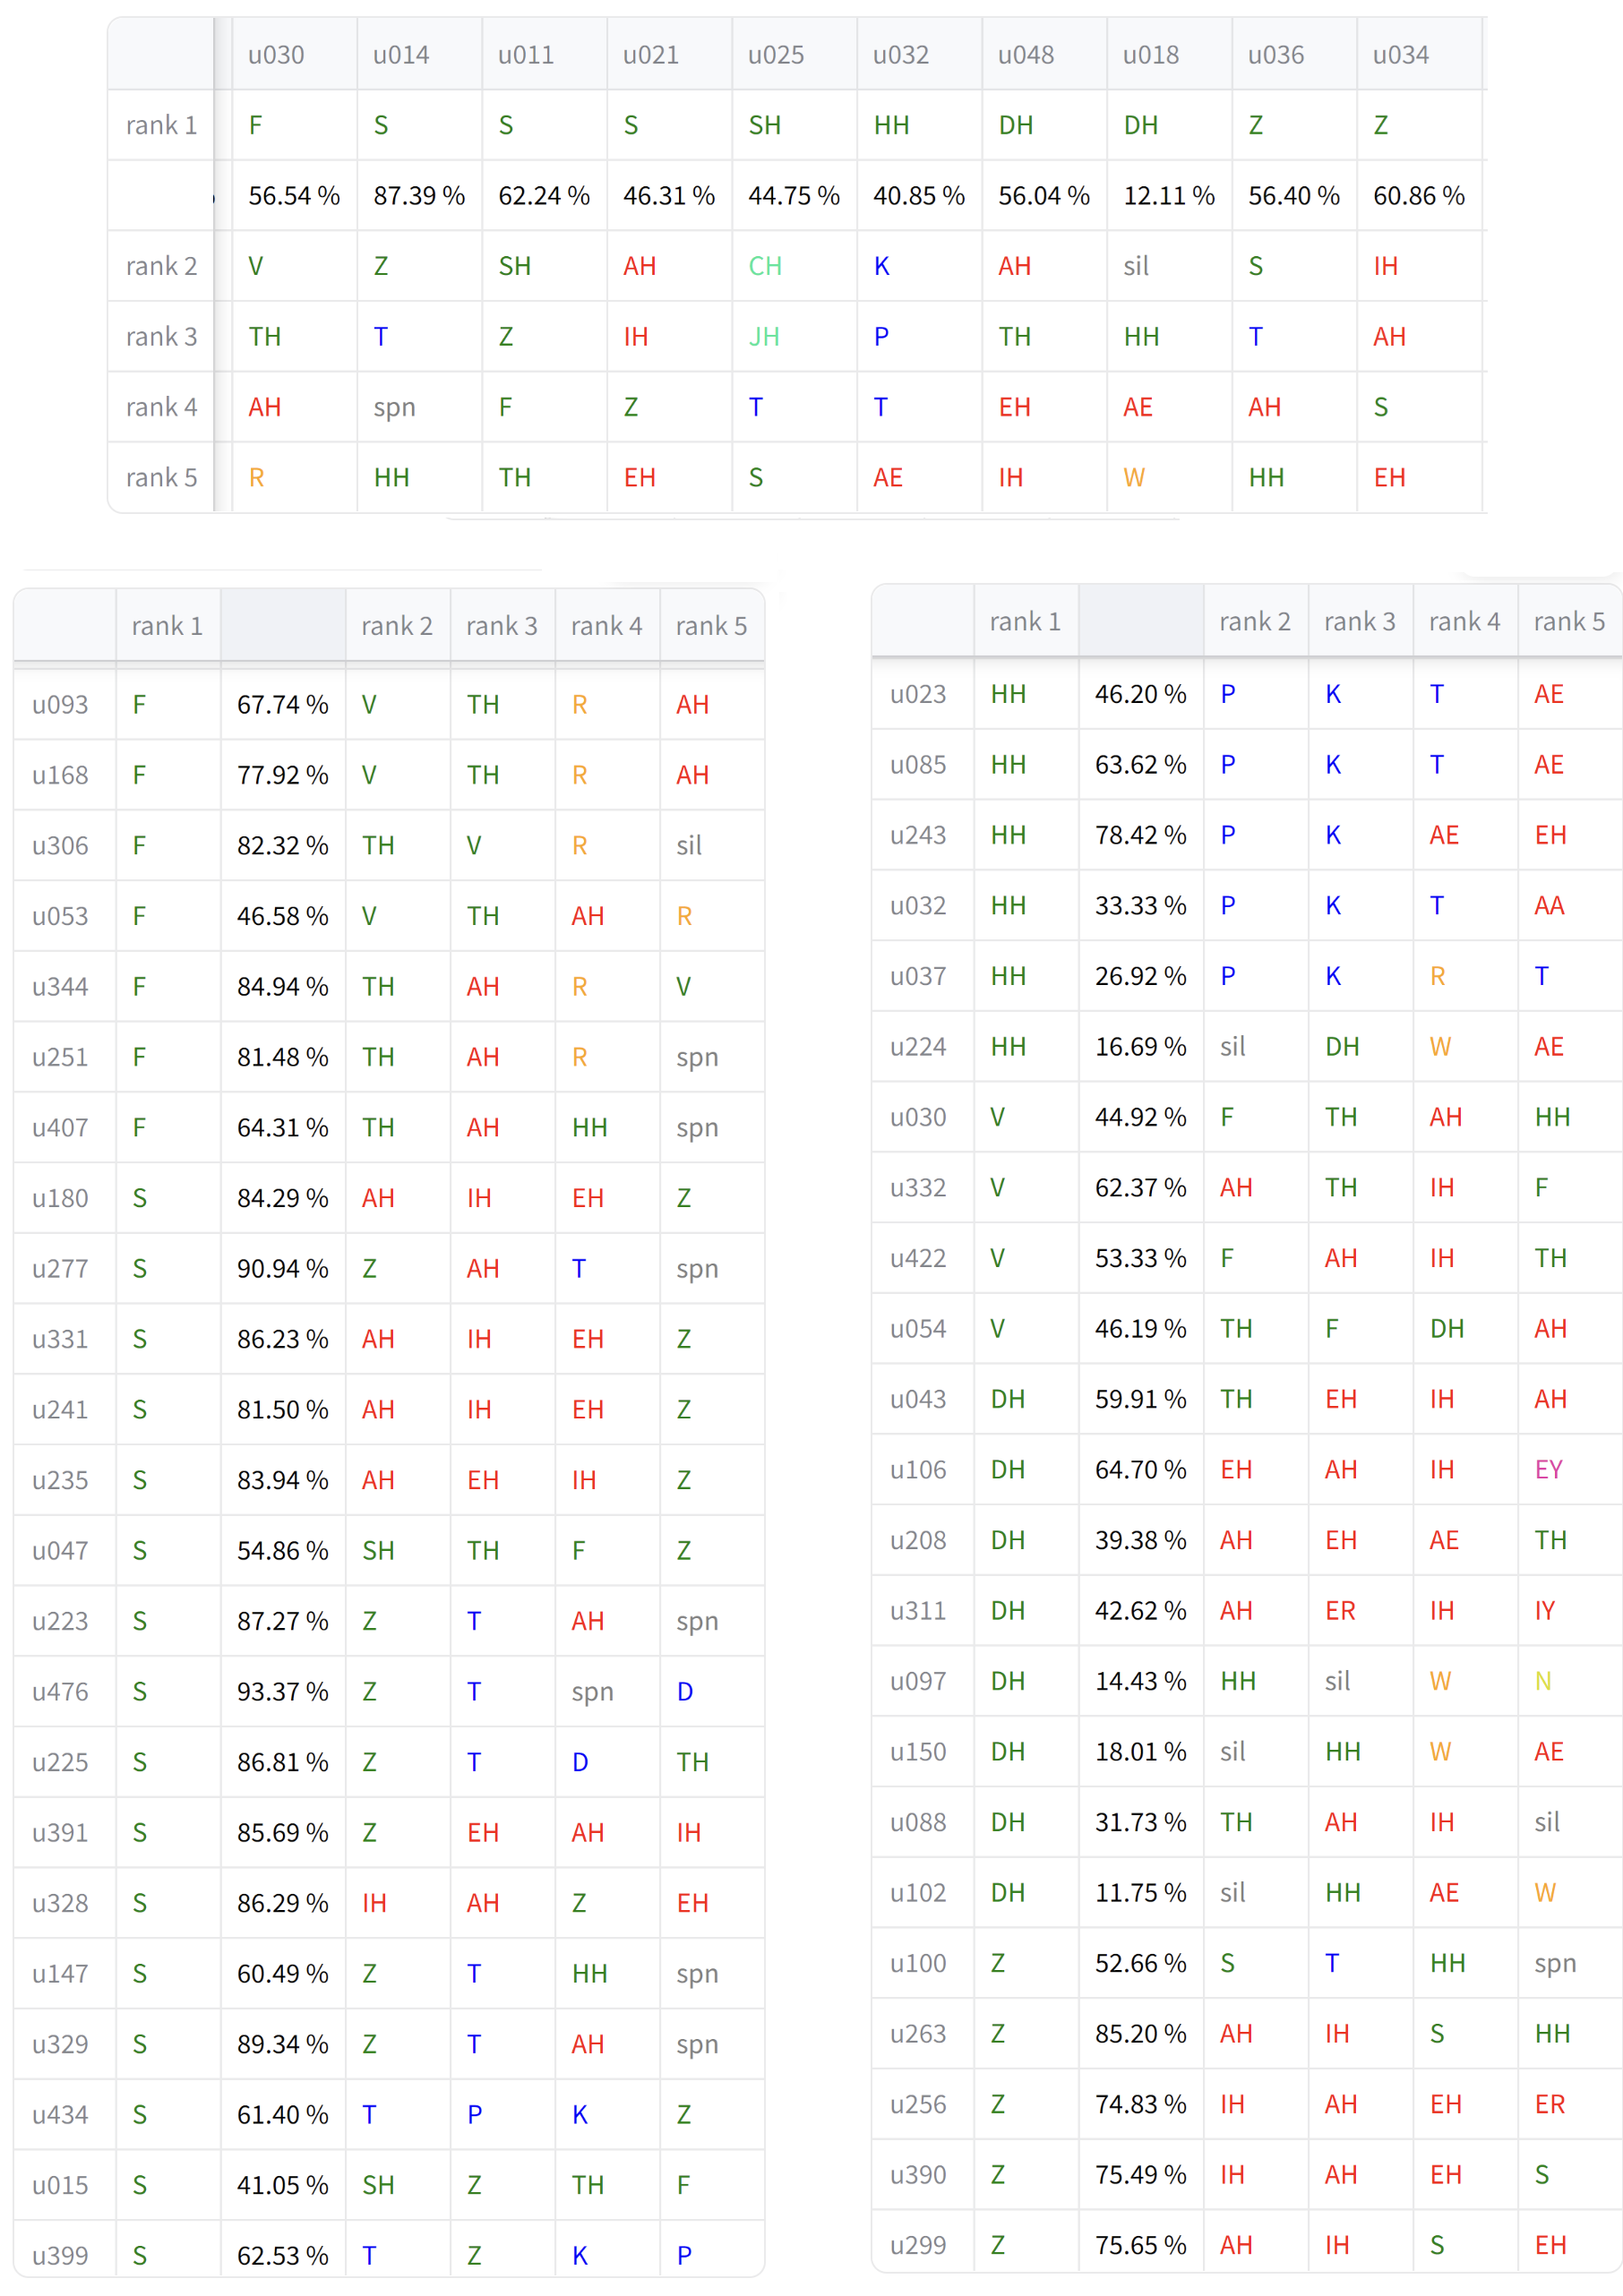
\includegraphics[width=\tempwidth]{figures/ch4figs/fri_phn.png}
             %     \caption{擦音}
             %     \label{fig:hub-u050-ap0500-friobs}
             % \end{subfigure}
             % \vfill
             % \begin{subfigure}{\textwidth}
             %     \centering
             %     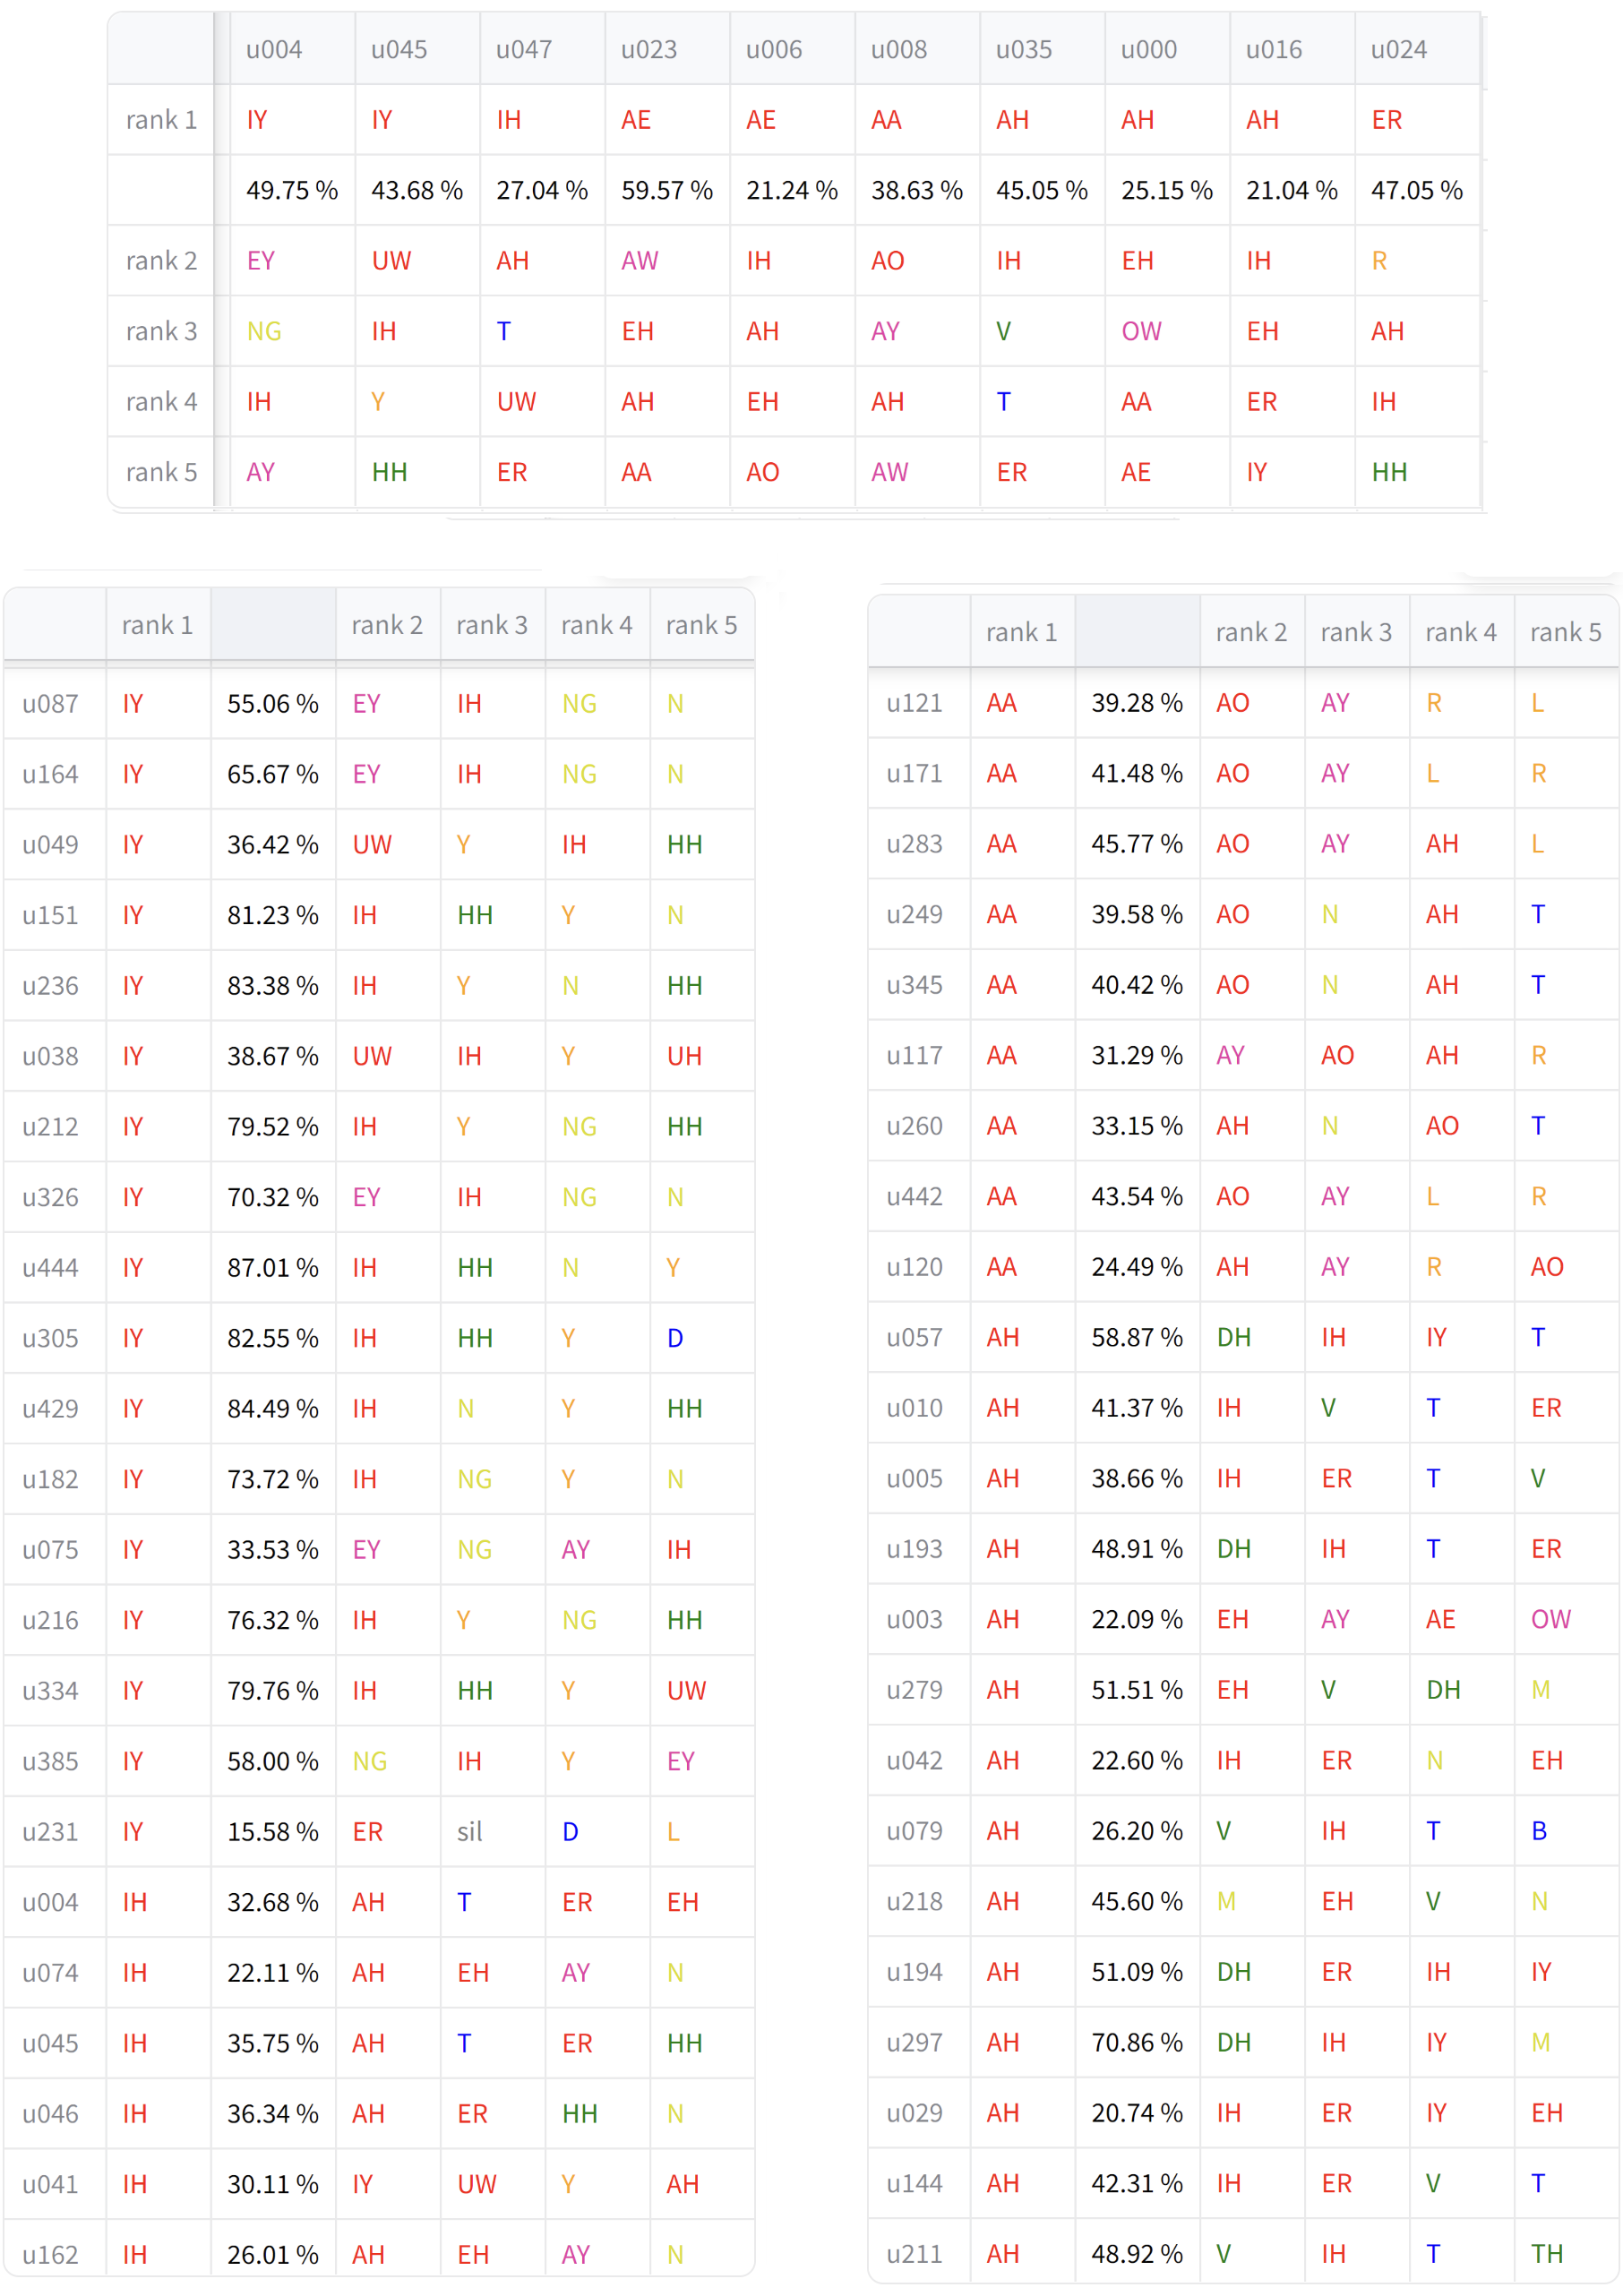
\includegraphics[width=\tempwidth]{figures/ch4figs/vow_phn.png}
             %     \caption{單元音}
             %     \label{fig:hub-u050-ap0500-vowobs}
             % \end{subfigure}

             \caption{HuBERT 表徵、K-平均演算法分群數 50,比較單一離散單元與}
             使用 500 種次詞單位,依據不同音位分類比較符記各自對應的前五高音位 \\
             上半部為離散單元,下半部為聲學片段。 \\
             圖中的百分比為最高機率音位的條件機率 $p_{y|z}(i^*(j)|j)$
                         \label{fig:hub-u050-phnobserver}
        \end{figure}
    }

        {
        \newcommand{\tempwidth}[0]{0.8\linewidth}
        \begin{figure}
        \ContinuedFloat
             \centering
             % \begin{subfigure}{\textwidth}
             %     \centering
             %     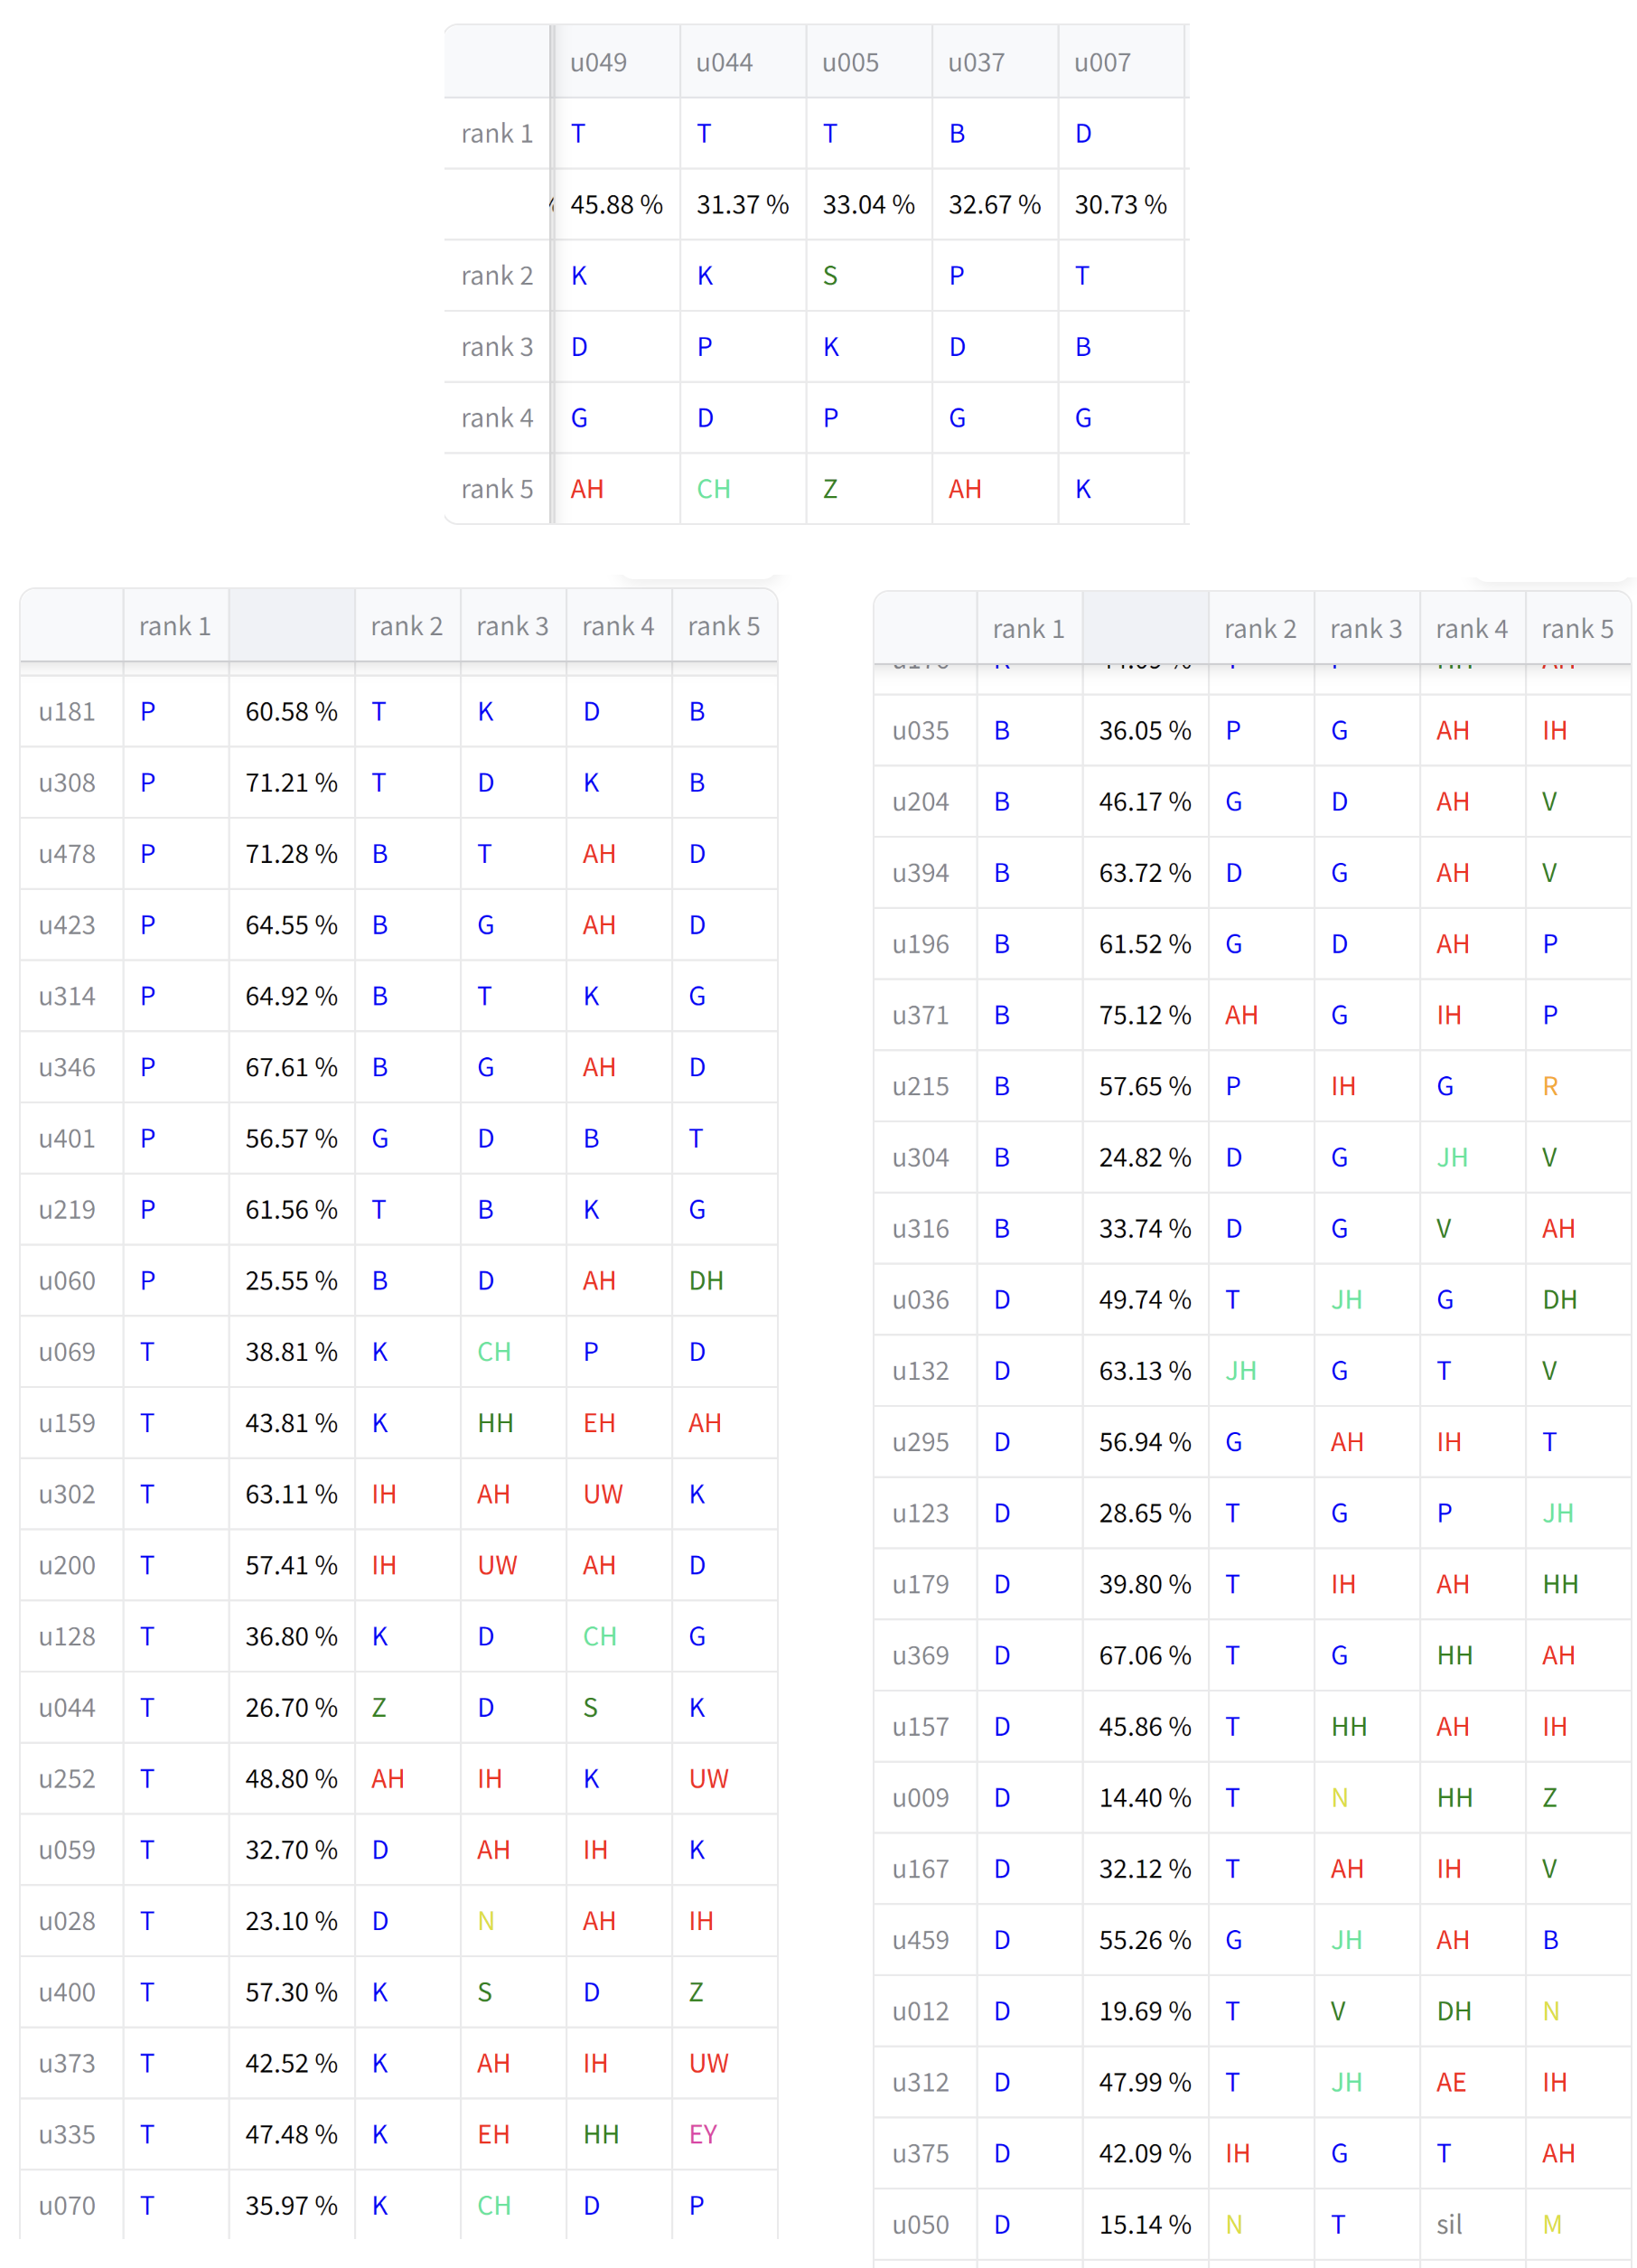
\includegraphics[width=\tempwidth]{figures/ch4figs/plo_phn.png}
             %     \caption{塞音}
             %     \label{fig:hub-u050-ap0500-ploobs}
             % \end{subfigure}
             % \vfill
             \begin{subfigure}{\textwidth}
                 \centering
                 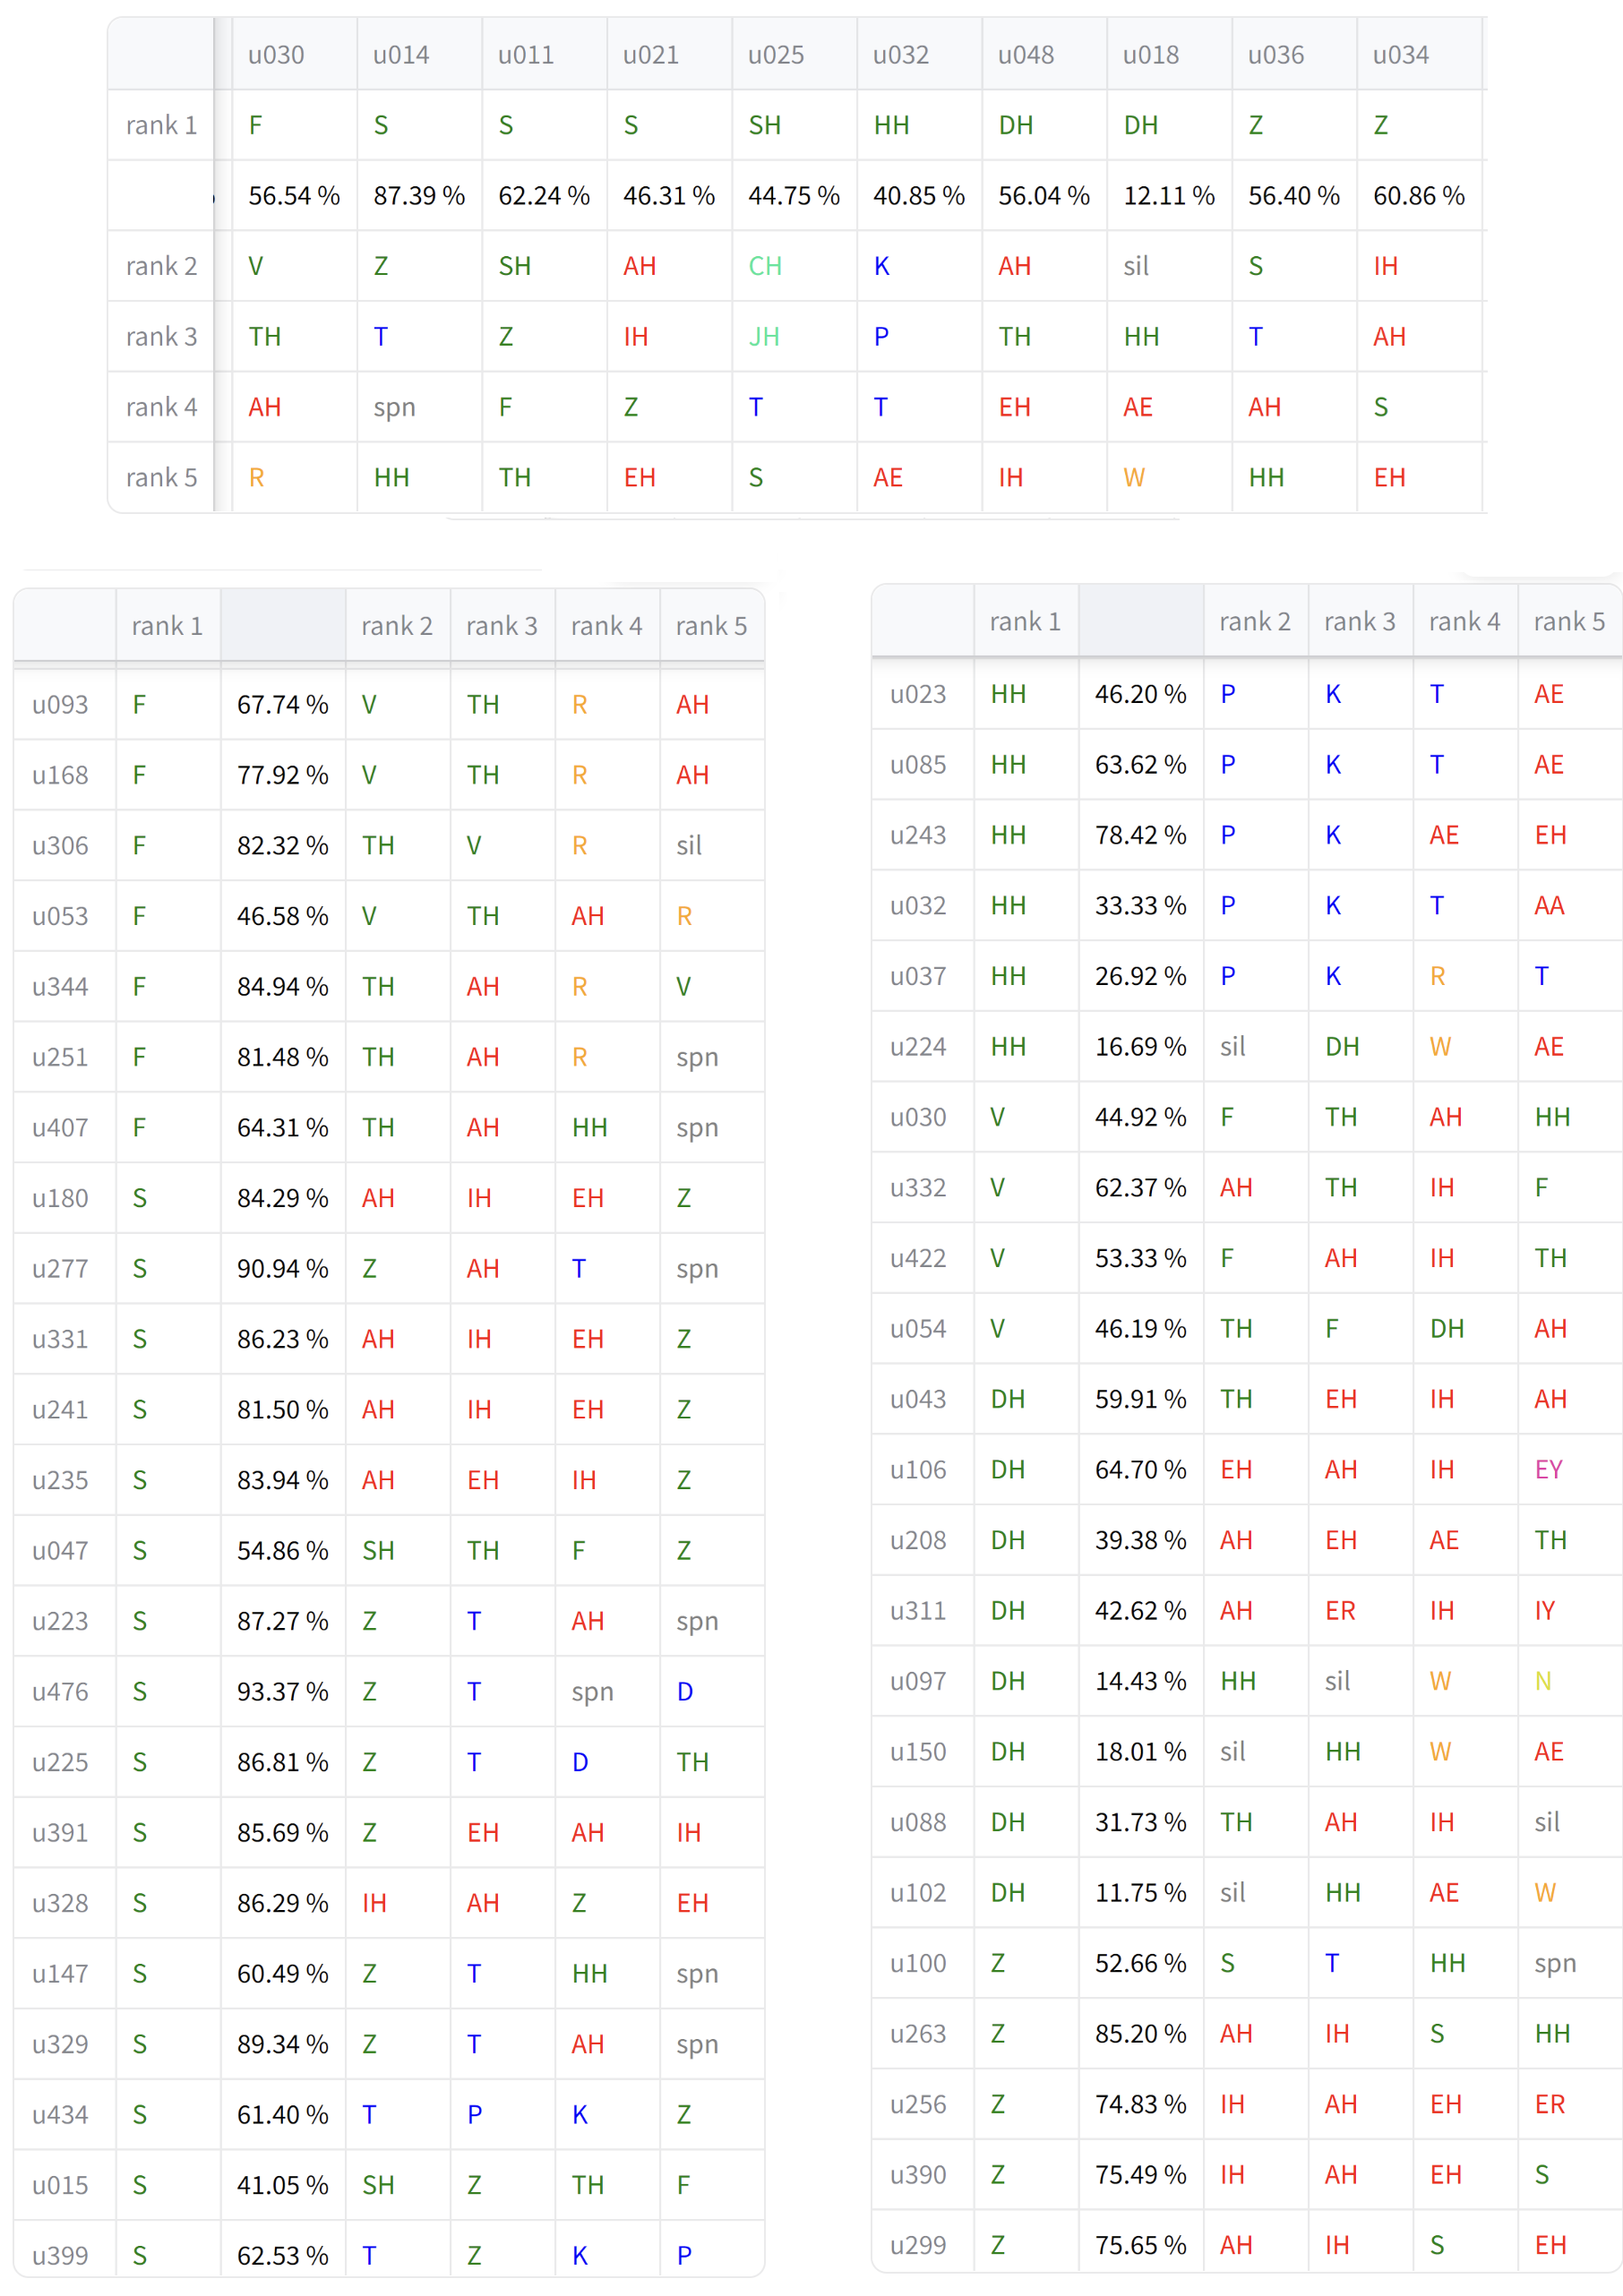
\includegraphics[width=\tempwidth]{figures/ch4figs/fri_phn.png}
                 \caption{擦音}
                 \label{fig:hub-u050-ap0500-friobs}
             \end{subfigure}
             % \vfill
             % \begin{subfigure}{\textwidth}
             %     \centering
             %     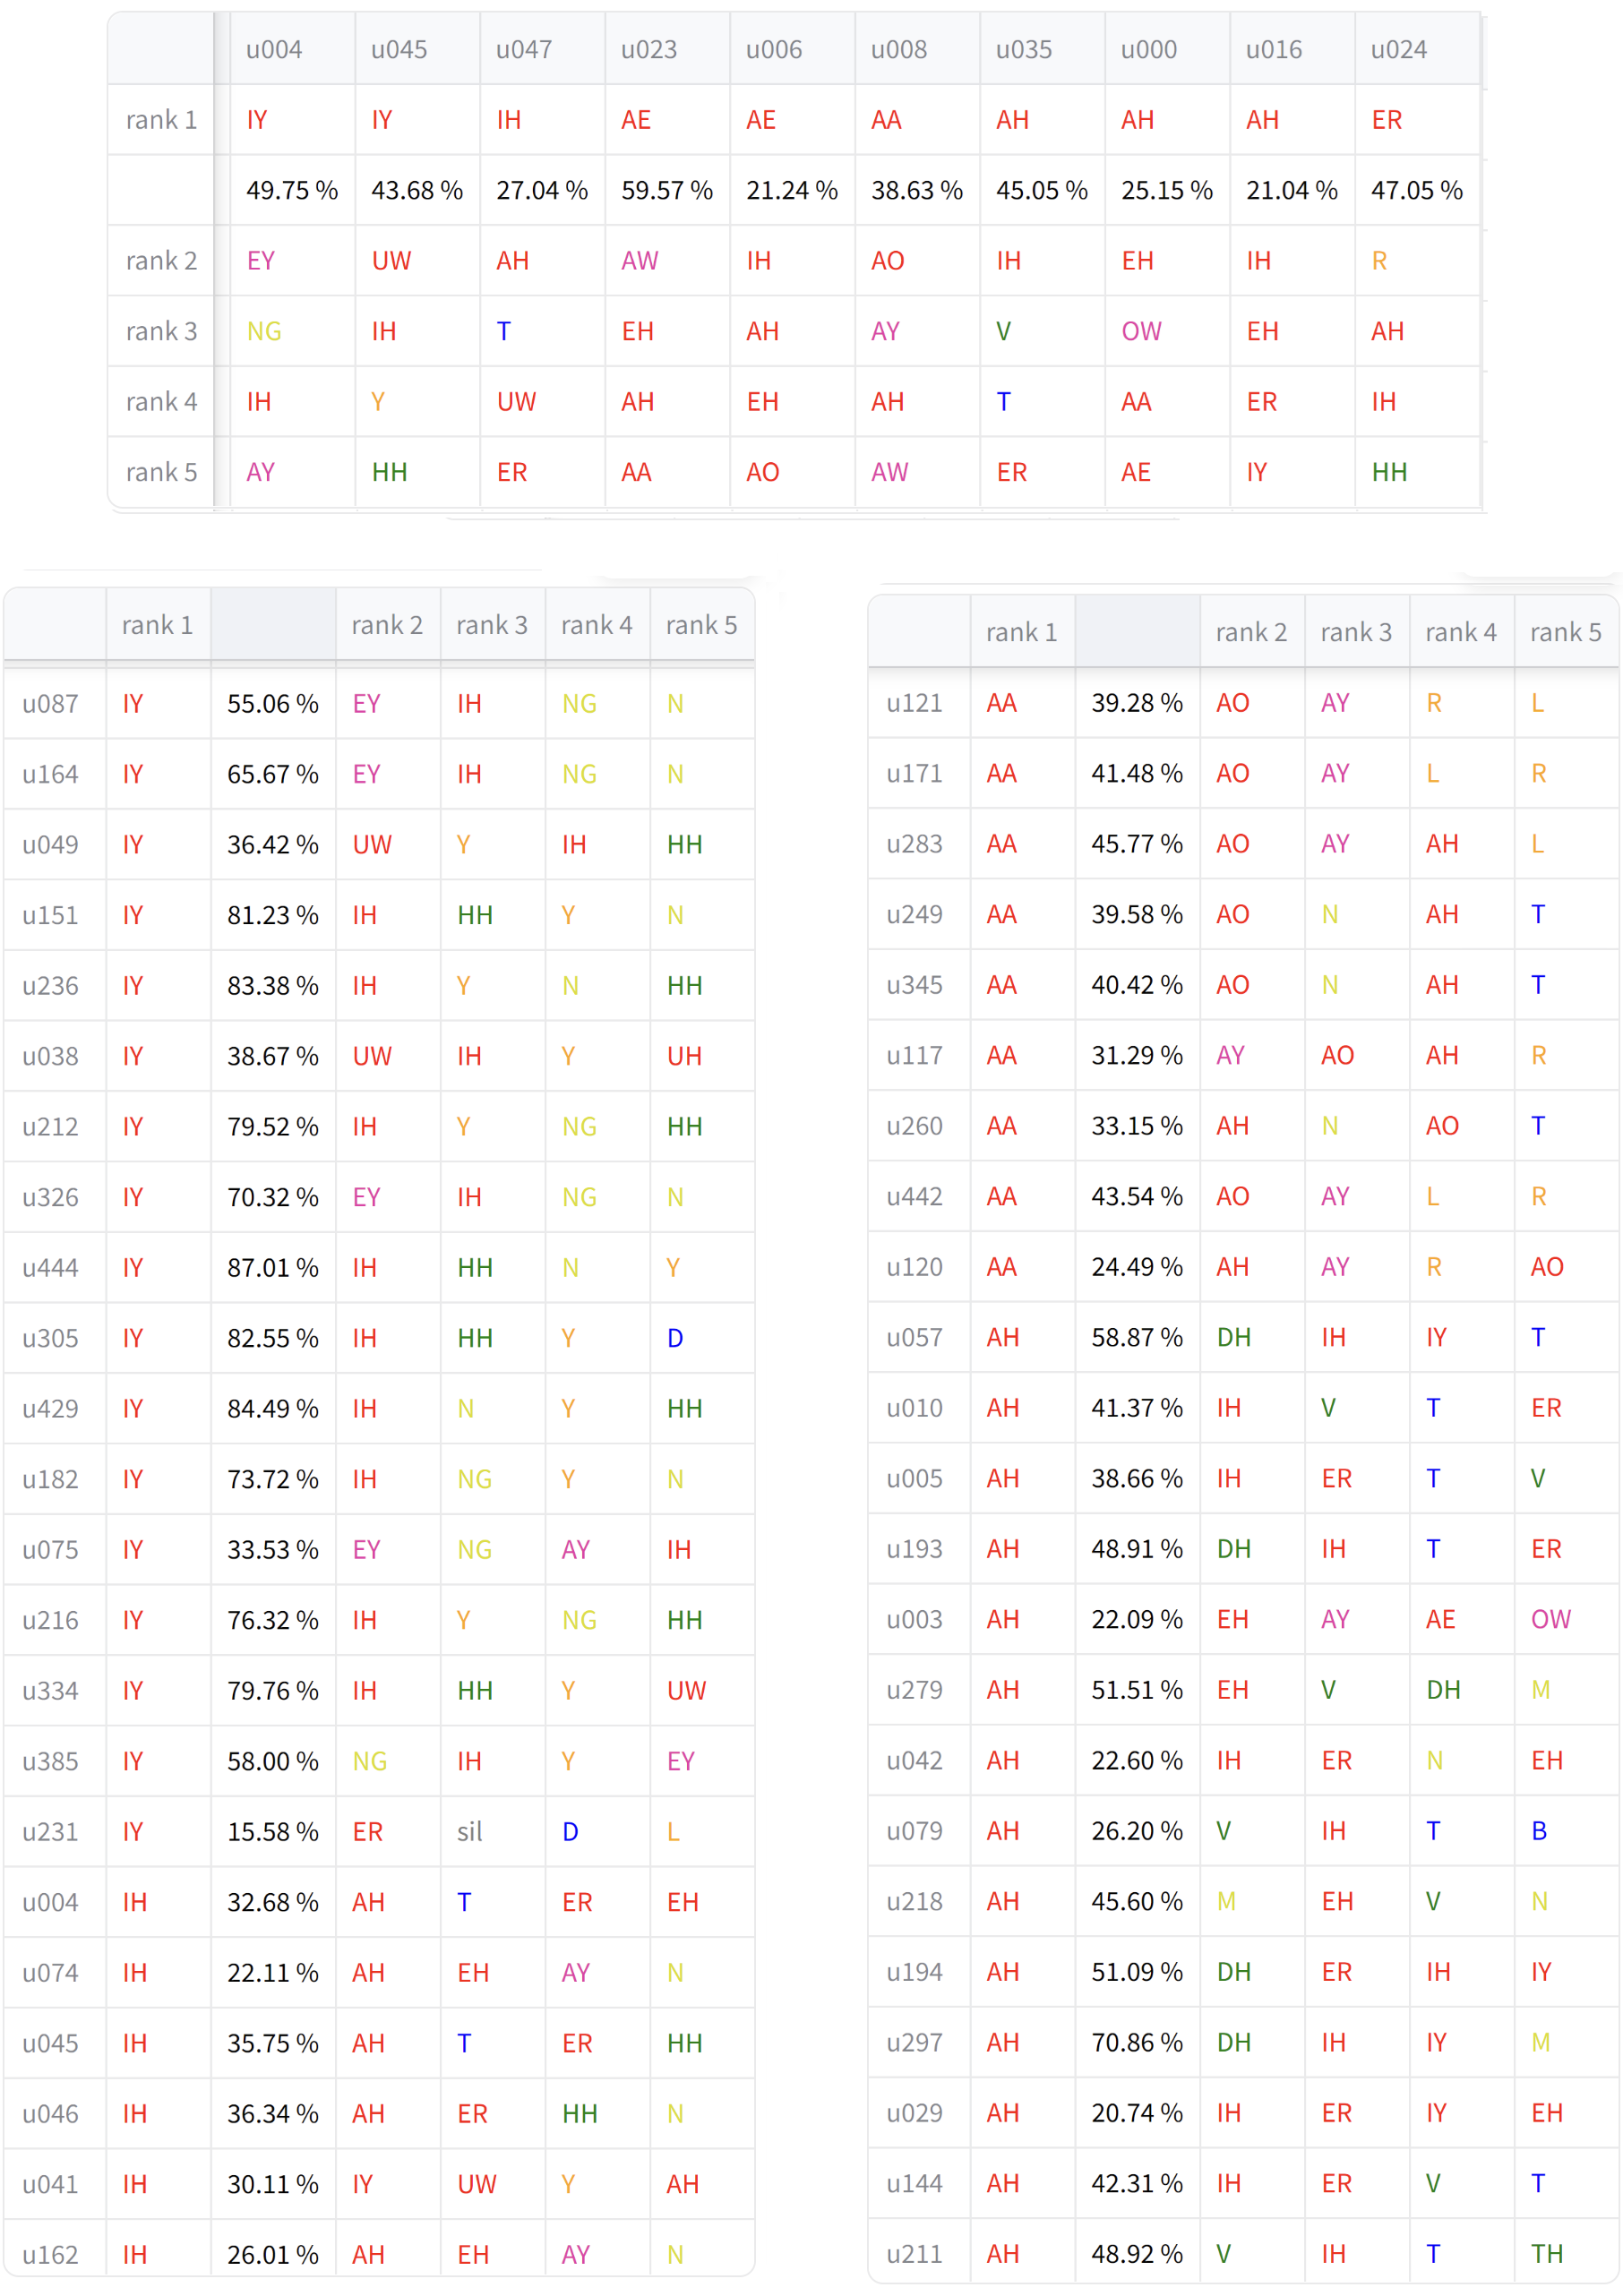
\includegraphics[width=\tempwidth]{figures/ch4figs/vow_phn.png}
             %     \caption{單元音}
             %     \label{fig:hub-u050-ap0500-vowobs}
             % \end{subfigure}

             % \caption{HuBERT 表徵、K-平均演算法分群數 50,比較單一離散單元與使用 500 種次詞單位,}
             % 依據不同音位分類比較符記各自對應的前五高音位
             % (上半部為離散單元,下半部為聲學片段。圖中的百分比為最高機率音位的條件機率 $p_{y|z}(i^*(j)|j)$)
                         \label{fig:hub-u050-phnobserver--2}
        \end{figure}
    }

        {
        \newcommand{\tempwidth}[0]{0.8\linewidth}
        \begin{figure}
        \ContinuedFloat
        
             \centering
             % \begin{subfigure}{\textwidth}
             %     \centering
             %     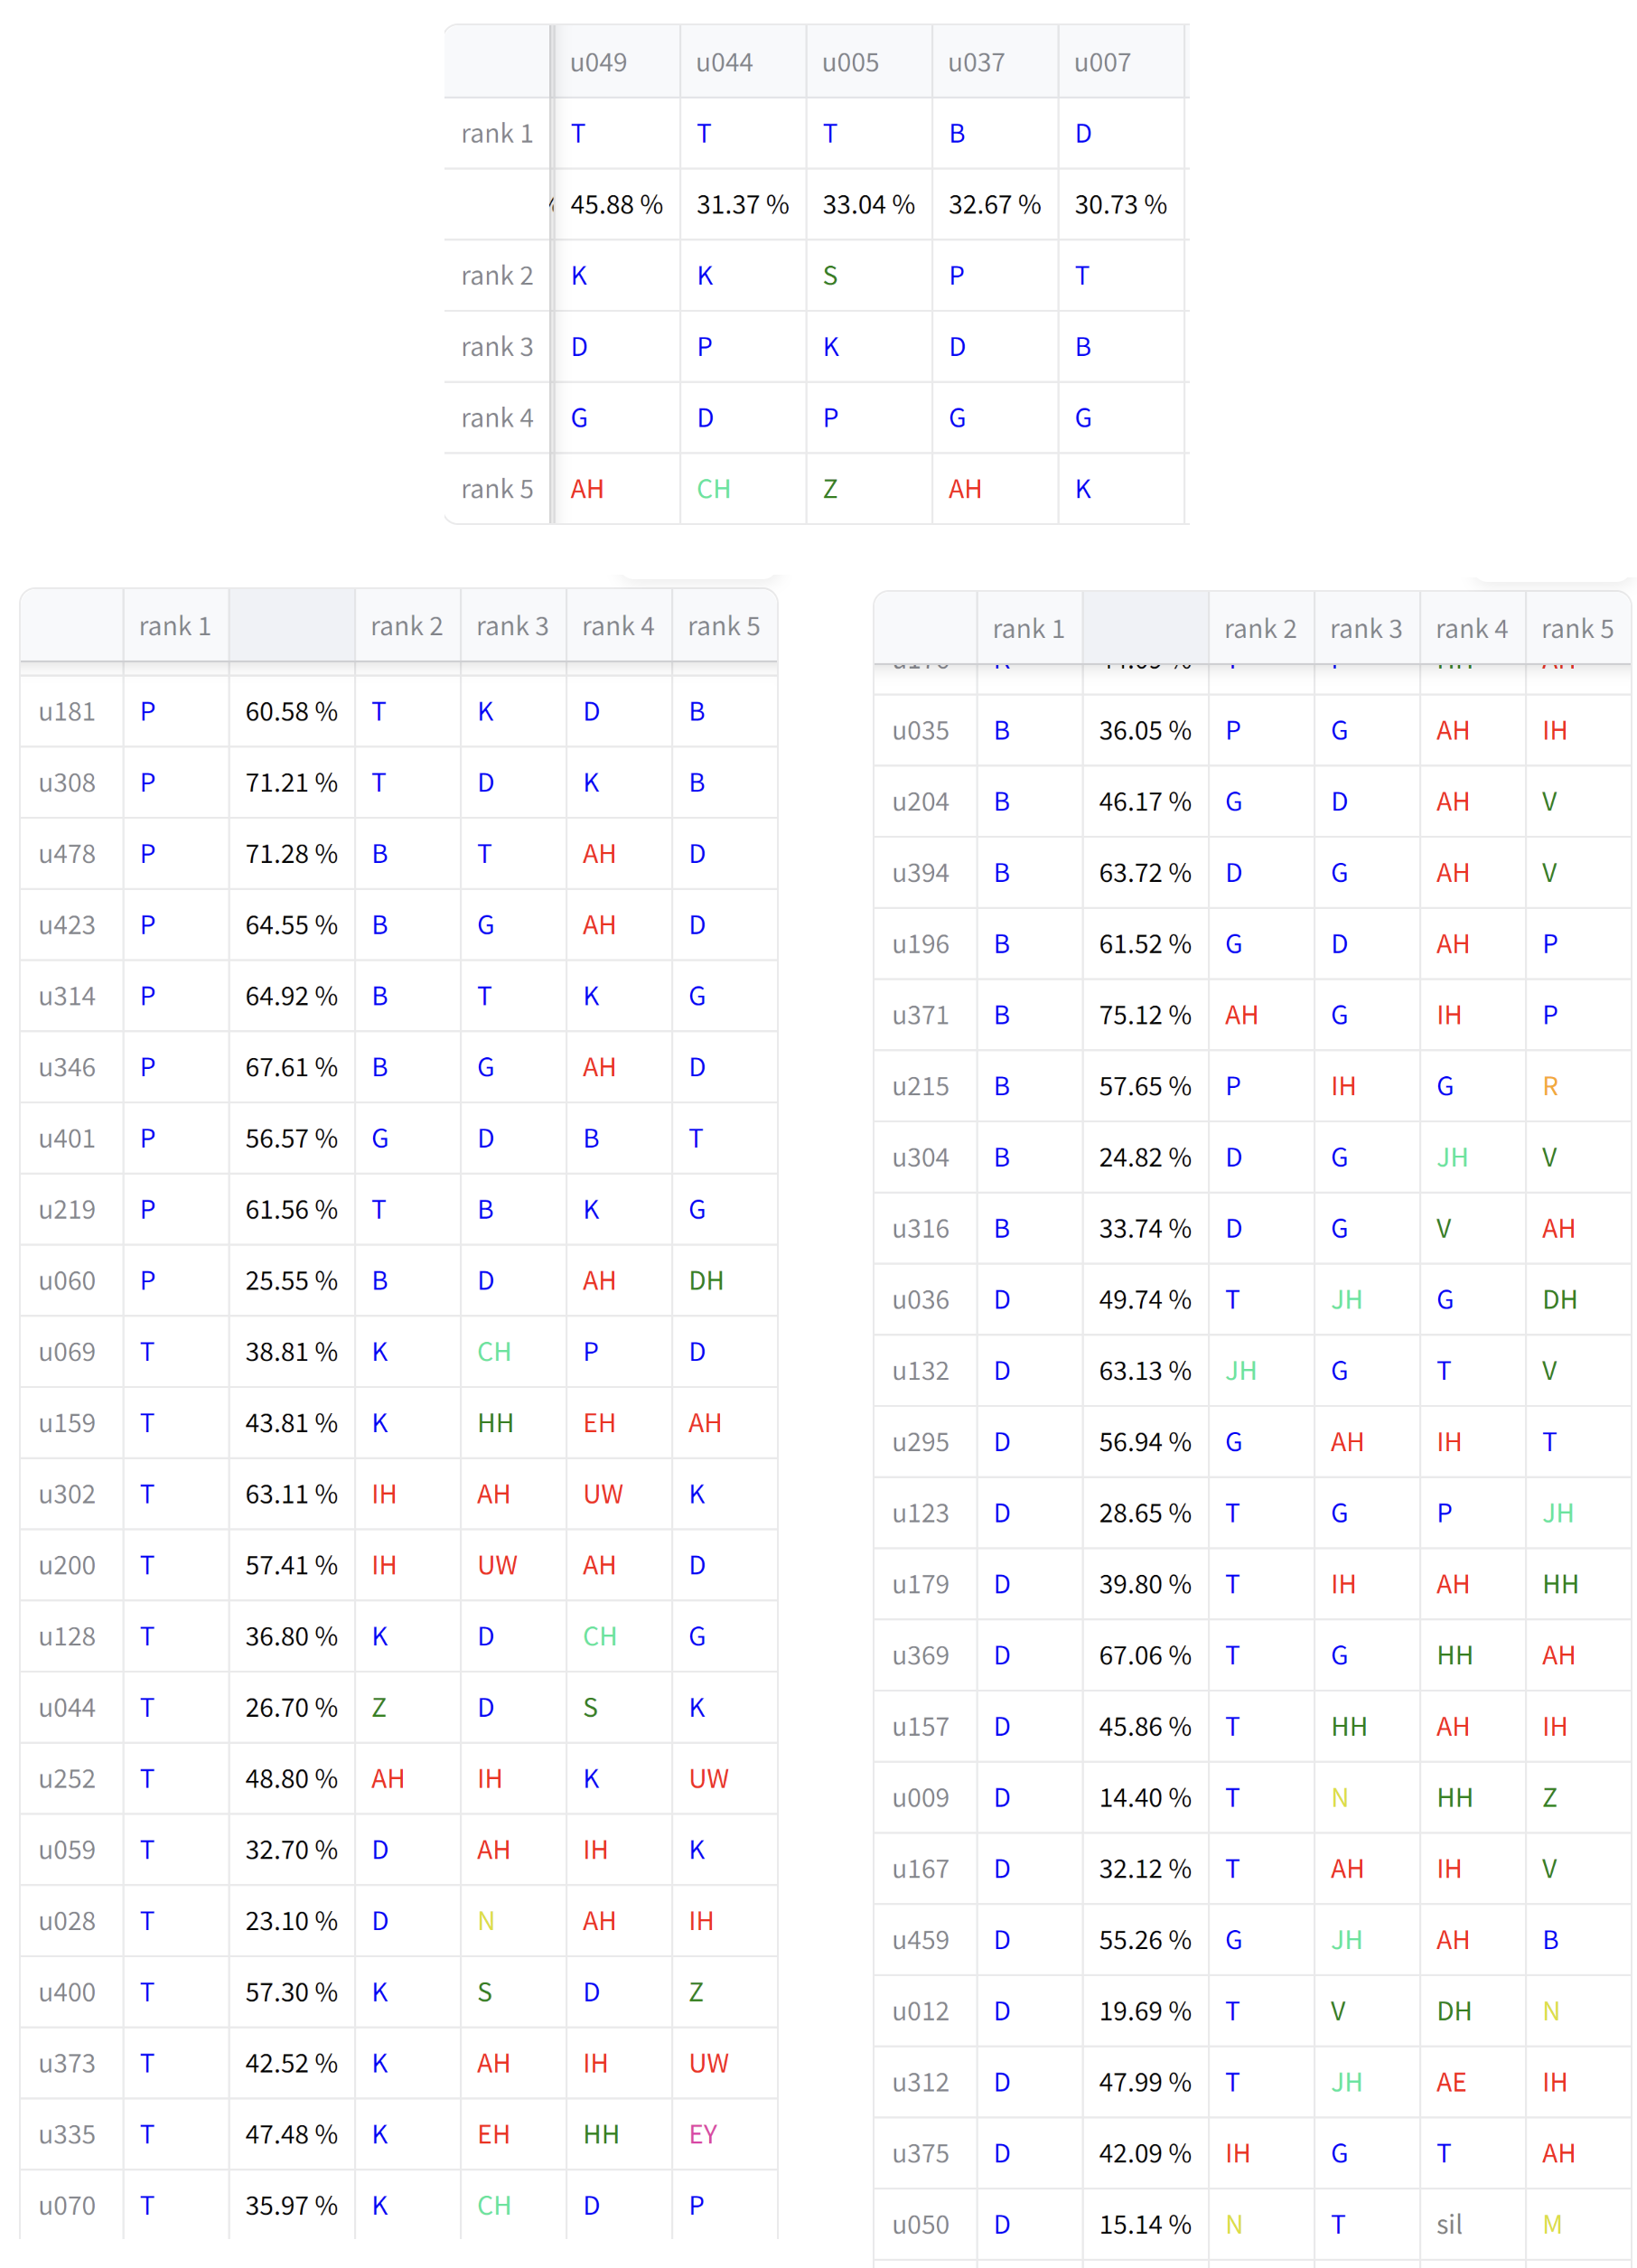
\includegraphics[width=\tempwidth]{figures/ch4figs/plo_phn.png}
             %     \caption{塞音}
             %     \label{fig:hub-u050-ap0500-ploobs}
             % \end{subfigure}
             % \vfill
             % \begin{subfigure}{\textwidth}
             %     \centering
             %     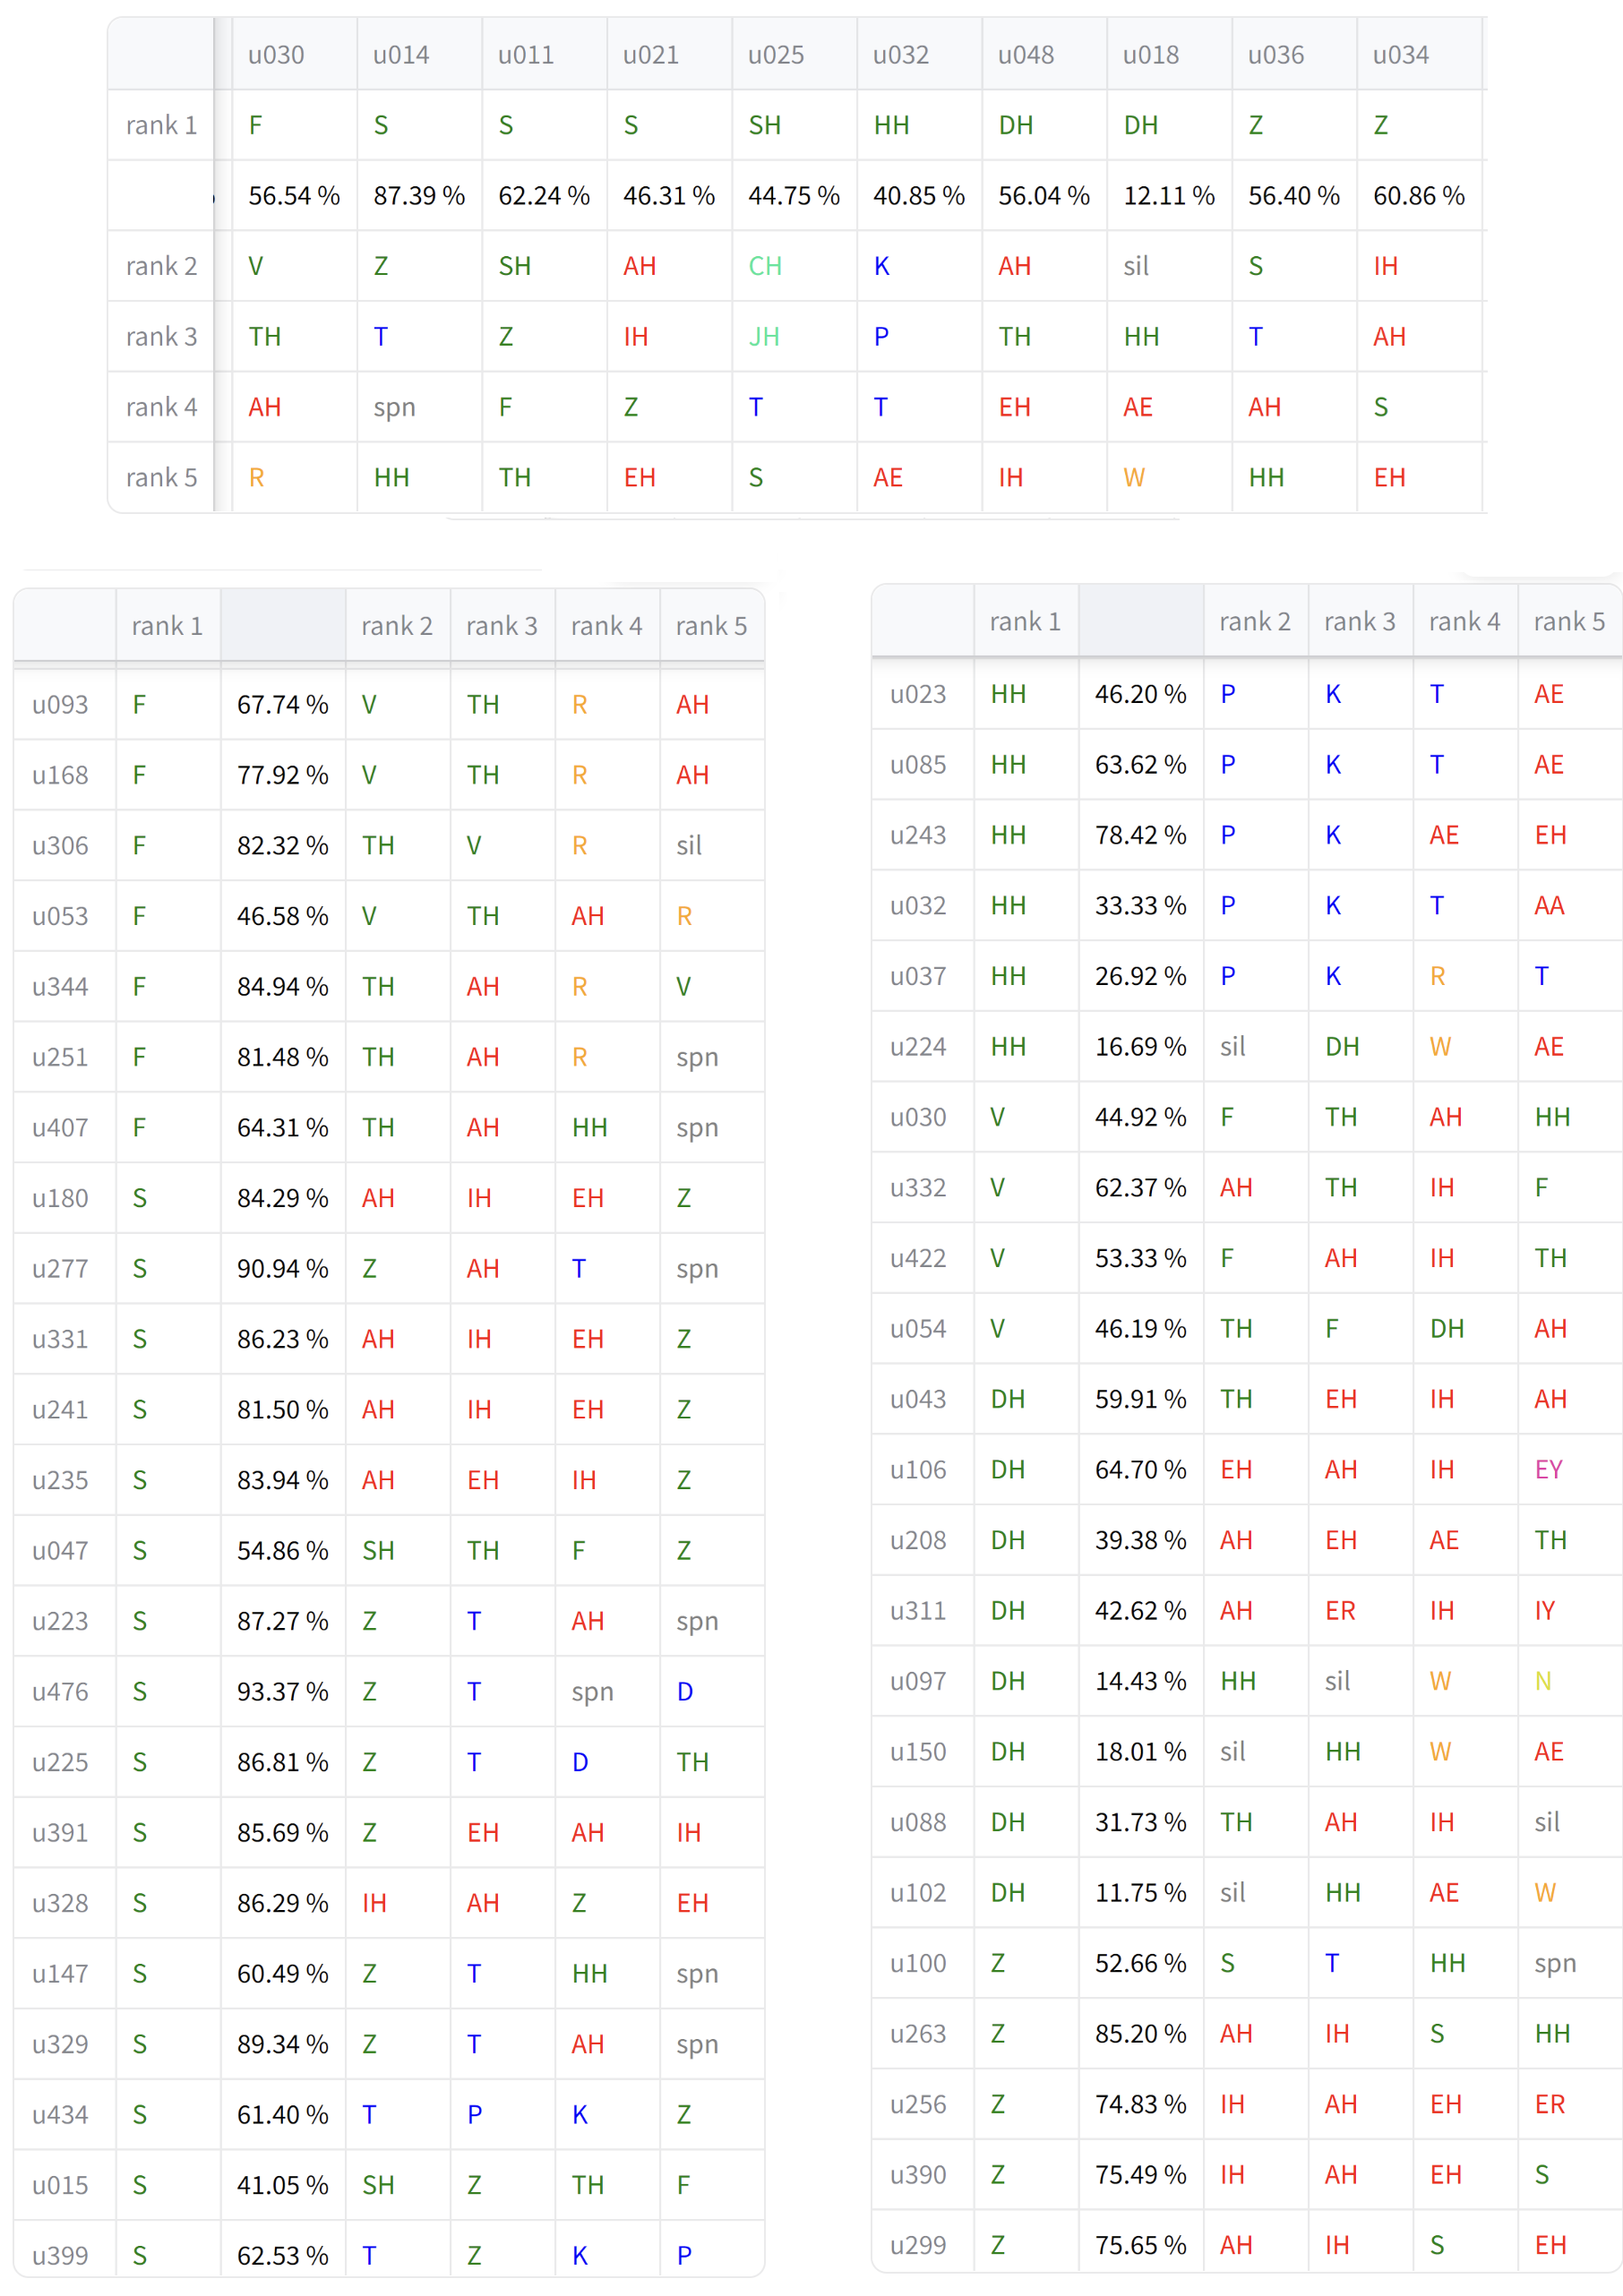
\includegraphics[width=\tempwidth]{figures/ch4figs/fri_phn.png}
             %     \caption{擦音}
             %     \label{fig:hub-u050-ap0500-friobs}
             % \end{subfigure}
             % \vfill
             \begin{subfigure}{\textwidth}
                 \centering
                 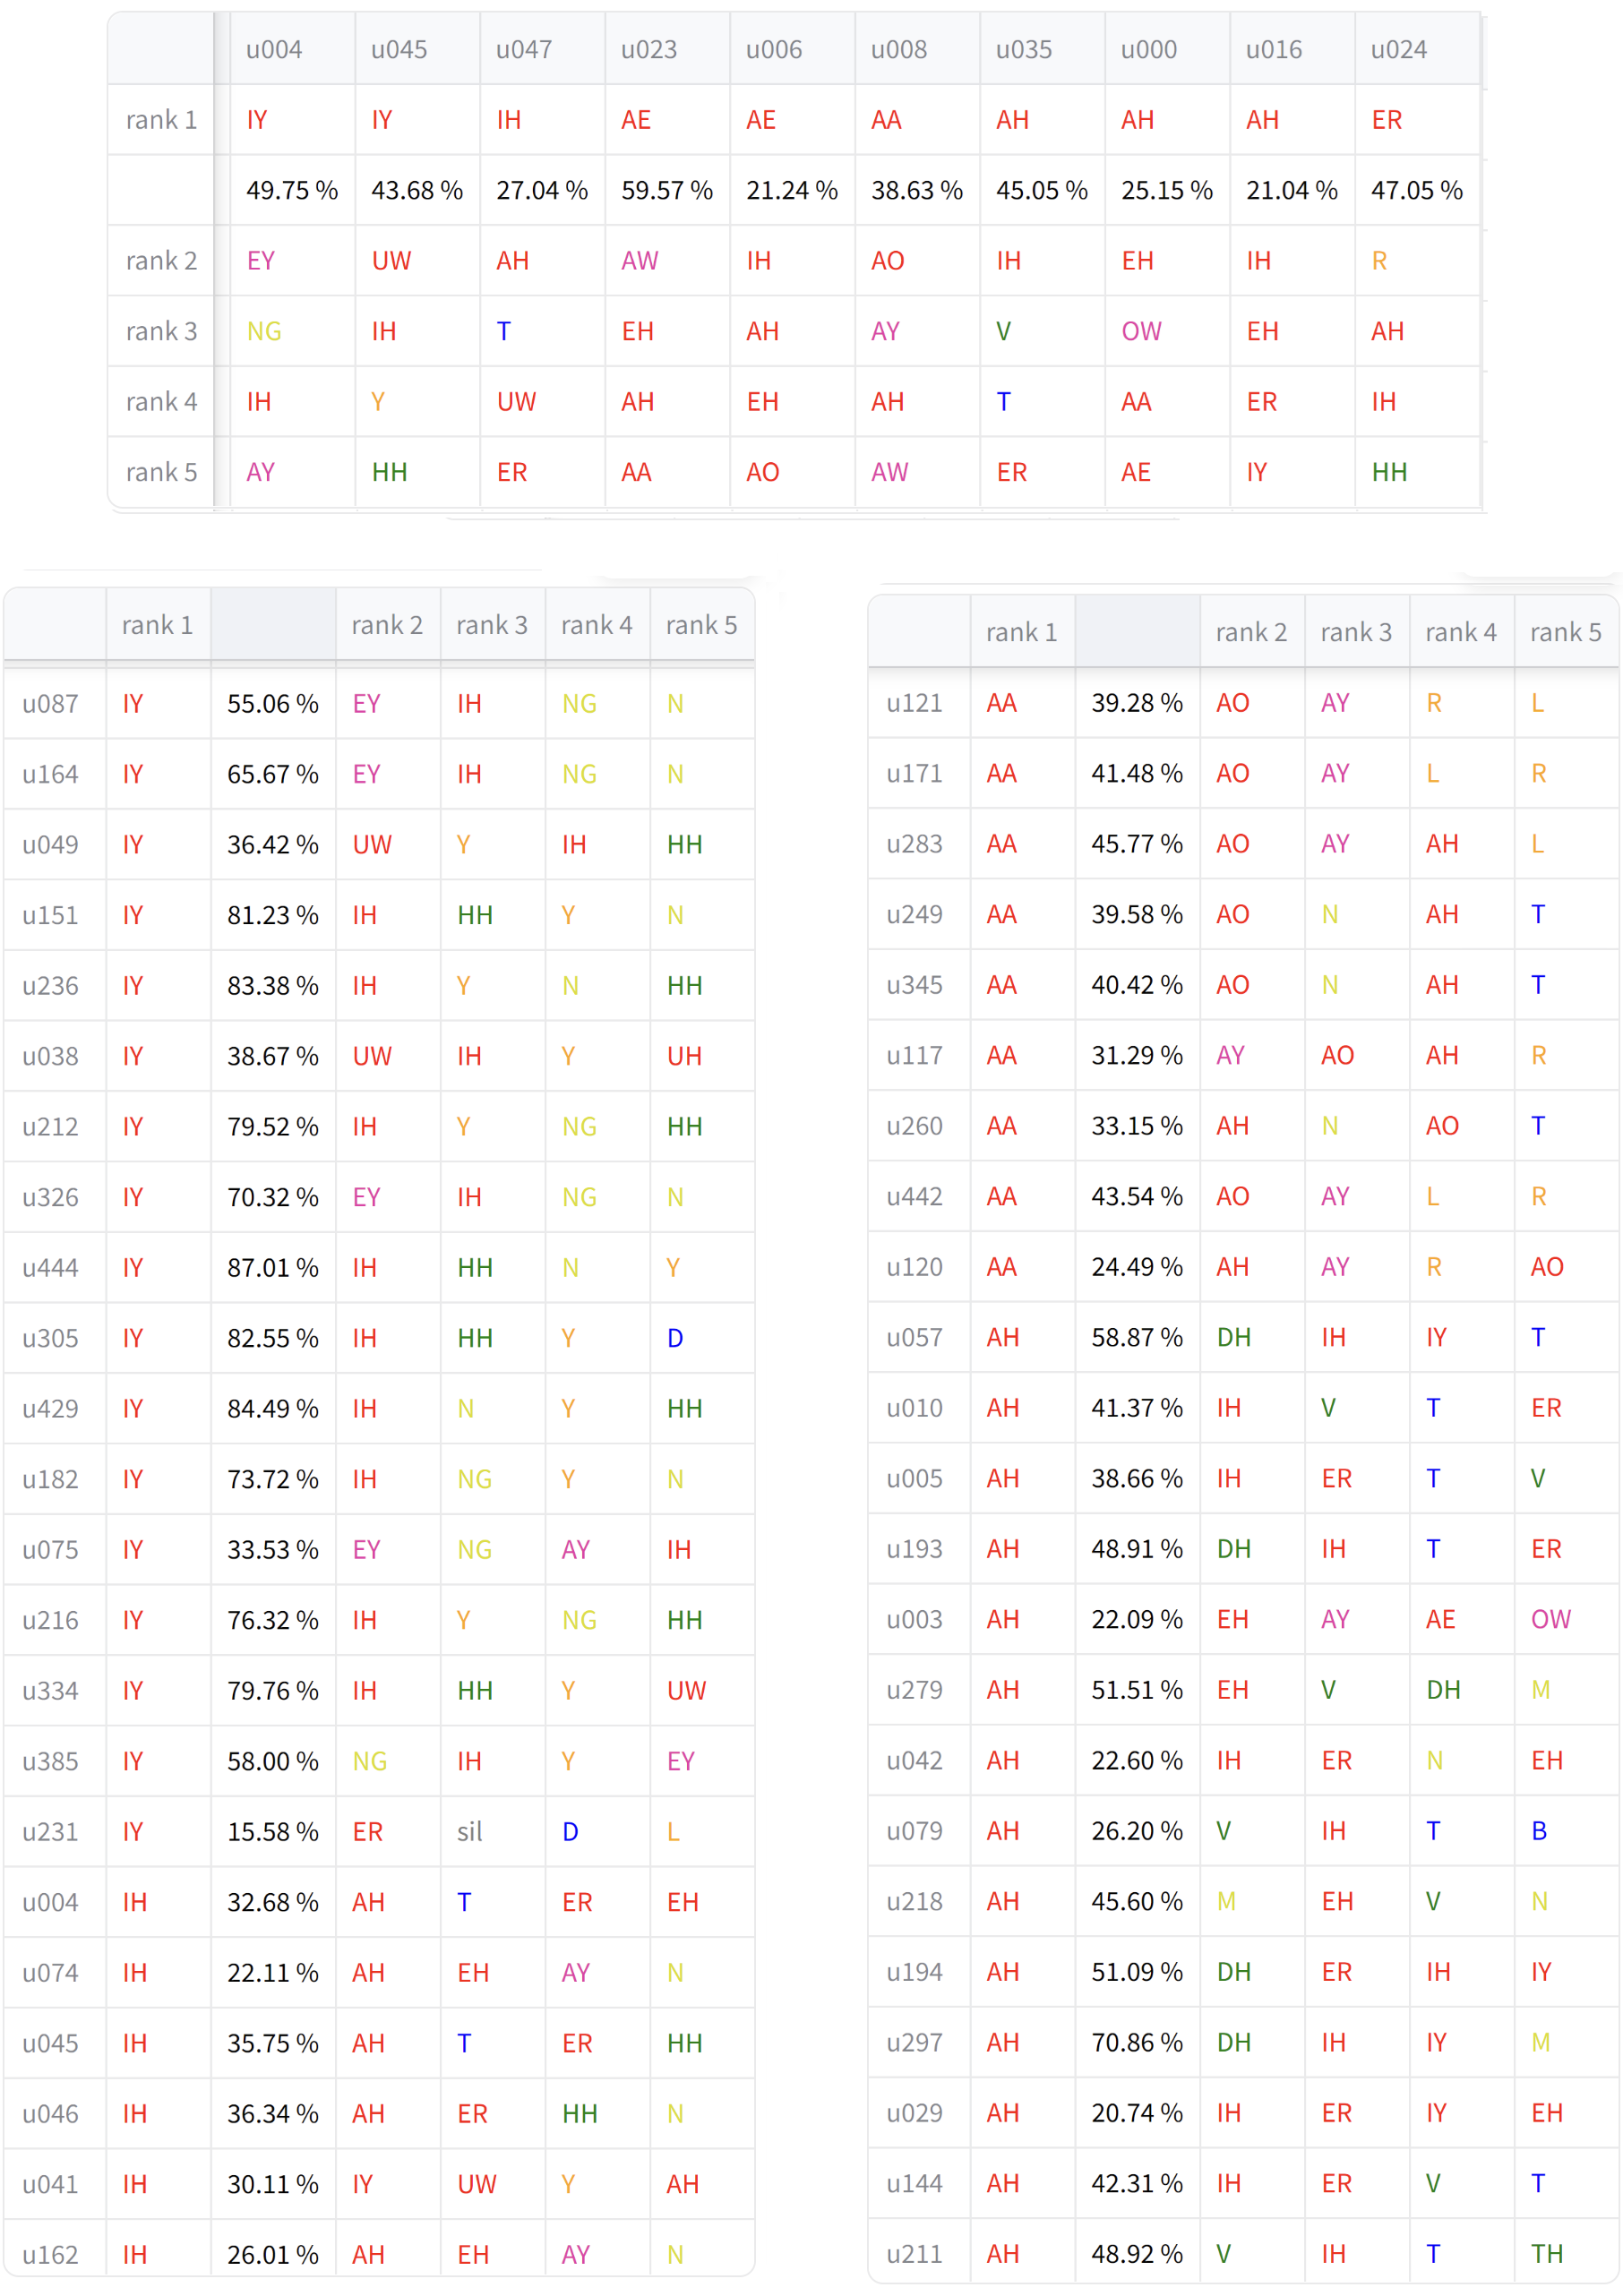
\includegraphics[width=\tempwidth]{figures/ch4figs/vow_phn.png}
                 \caption{單元音}
                 \label{fig:hub-u050-ap0500-vowobs}
             \end{subfigure}

             % \caption{HuBERT 表徵、K-平均演算法分群數 50,比較單一離散單元與使用 500 種次詞單位,}
             % 依據不同音位分類比較符記各自對應的前五高音位
             % (上半部為離散單元,下半部為聲學片段。圖中的百分比為最高機率音位的條件機率 $p_{y|z}(i^*(j)|j)$)
                         \label{fig:hub-u050-phnobserver--3}
        \end{figure}
    }

\subsubsection{聲學片段對應最高機率之音位間的比較}

  接下來,我們比較各個聲學片段與音位之間的對應關係,亦即每個符記所對應最可能的前幾個音位之間,是否依然如離散單元那樣存在特定特徵。觀察以 HuBERT 模型、分群數 50 為基礎,分別以「離散單元」與「500 種次詞單位的聲學片段」為符記的虛擬文字文本,將對應到
塞音、擦音和單元音
部分的次詞單位取出觀察,將每個符記
對應前五高機率的音位排名呈現在
圖 \ref{fig:hub-u050-phnobserver} 中(並附上最高機率音位 $i^*(j)$ 的條件機率值 $p_{y|z}(i^*(j)|j)$),圖中上半部是離散單元,下半部則是聲學片段的結果。
相互比較後可以發現,由於聲學片段的符記數量比離散單元更多,因此在維持對應音位之間相關性的同時,卻能呈現出不同音位間更細節的相關性。例如在圖 \ref{fig:hub-u050-ap0500-ploobs} 中,上半部顯示原先以離散單元為符記時,因為只有 50 種符記,因此只能看出 T、B 與 D 比較容易和哪些其他音位比較相關,但聲學片段卻可以呈現出 P、T、B、D 等更多細節的音位關係。
特別值得注意的是,圖 \ref{fig:aff} 是對應到塞擦音的幾個聲學片段,這些對應到 CH 和 JH 兩種塞擦音的聲學片段也確實給予了同樣是塞擦音的其他音位較高的機率。
    % (aff 圖)
    \begin{figure}
        \centering
        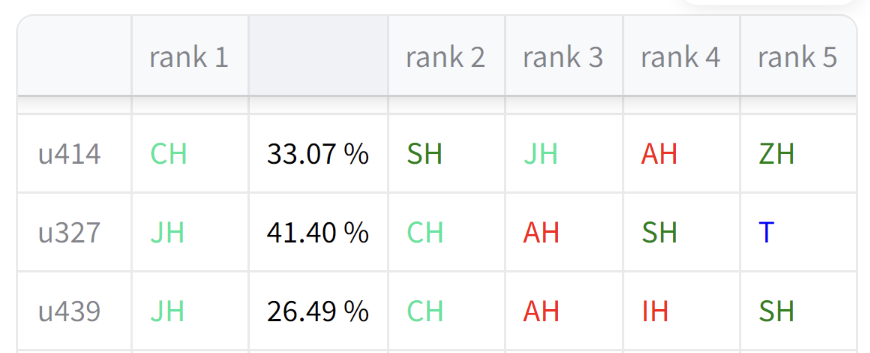
\includegraphics[width=0.8\linewidth]{figures/ch4figs/aff-hub50-500.png}
        \caption{對 HuBERT 分群數 50 離散單元取得 500 種次詞單位後,}
        對應到塞擦音的聲學片段之音位條件機率排名
        \label{fig:aff}
    \end{figure}


\begin{table}[!htbp]
    \centering
    
    \begin{subtable}[t]{\textwidth}
        \centering
        \begin{tabular}{|c|c|c|} \hline 
                符記種數& 音位分類純度& 以音位分類標註之分群純度\\ \hline 
               離散單元&   0.7006&  \textbf{0.1509}
\\ \hline 
                   500    &  0.7116&  0.0340
\\ \hline 
                  1000    &  \textbf{0.7186}&  0.0226
\\ \hline 
                  8000    &  0.7080&  0.0119
\\ \hline 
                 10000    &  0.7048&  0.0113
\\ \hline 
                 20000    &  0.6929&  0.0089\\ \hline 
        \end{tabular}
\caption{群數 = 50}
        \label{tab:ch4-new-hubert-pcls-clu050}
    \end{subtable}        

    \vfill        

    \begin{subtable}[t]{\textwidth}
        \centering
        \begin{tabular}{|c|c|c|} \hline 
                符記種數& 音位分類純度& 以音位分類標註之分群純度\\ \hline 
               離散單元&   \textbf{0.7584}&  \textbf{0.0882}\\ \hline 
                   500    &  0.7578&  0.0326
\\ \hline 
                  1000    &  0.7576&  0.0223
\\ \hline 
                  8000    &  0.7382&  0.0097
\\ \hline 
                 10000    &  0.7346&  0.0090
\\ \hline 
                 20000    &  0.7235&  0.0074
\\ \hline 
        \end{tabular}
\caption{群數 = 100}
        \label{tab:ch4-new-hubert-pcls-clu100}
    \end{subtable}    

\caption{HuBERT 模型在不同詞表大小時的語音學類別分析數據}
    \label{tab:new--hubert-pcls-results}
\end{table}

        仿照第三章,藉由以音位分類作為新的標註計算純度,我們可以確認聲學片段給予同類音位較高機率的效果。然而從表 \ref{tab:new--hubert-pcls-results} 可以發現,隨著符記種數的提升,僅有分群數 50 時在較少符記種類時,音位分類的純度有微幅提升,多數時候符記種數的提高,伴隨的反而是音位分類純度些微的降低。由此可以推斷,次詞單位的引入雖能帶來更多樣的符記,對應音位間的關係卻在 K-平均演算法得到的離散單元已經大致抵定,次詞單位帶來的效果幾乎已經沒什麼改善的空間。
        % \par
其理由很可能是源自次詞單位演算法的特性,聲學片段的計算過程可以把原先代表不同種類音位的離散單元合在一起。因此,即便整體新的符記對應音位的純度有所提升,對音位分類的相關性卻低上不少。  \jcm{phn pur up, but pcls pur down}

\subsection{由音位角度探討}


    {
        \newcommand{\tempwidth}[0]{0.8\linewidth}
        \begin{figure}
             \centering
             \begin{subfigure}{\textwidth}
                 \centering
                 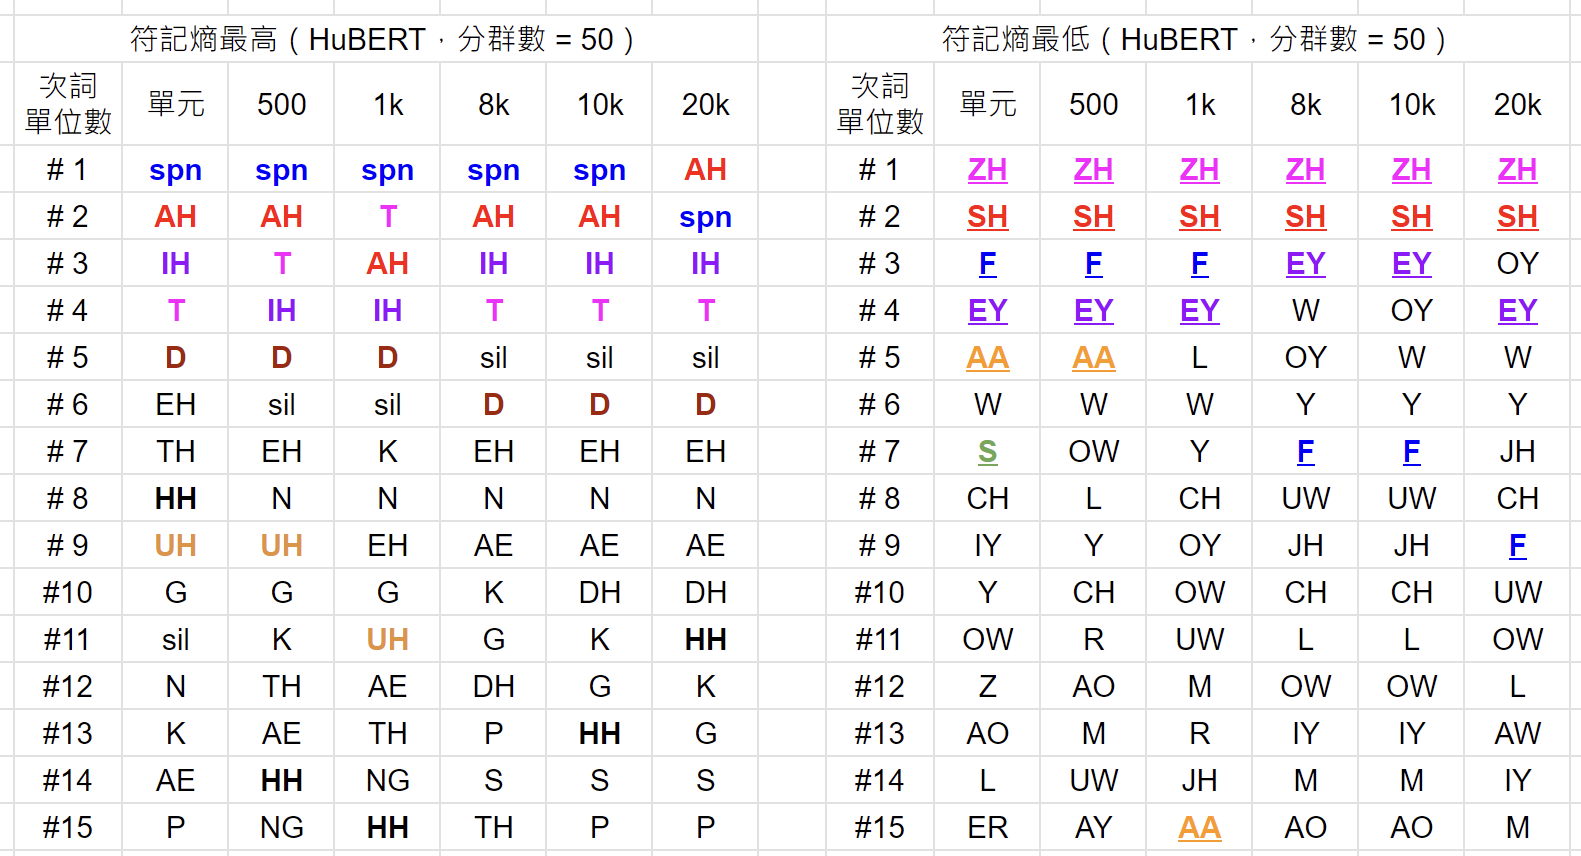
\includegraphics[width=\tempwidth]{figures/ch4figs/phnrank-hub50pcs.png}
                 \caption{分群數 = 50}
                 \label{fig:hub-u050-phnrank-hub50pcs}
             \end{subfigure}
             \vfill
             \begin{subfigure}{\textwidth}
                 \centering
                 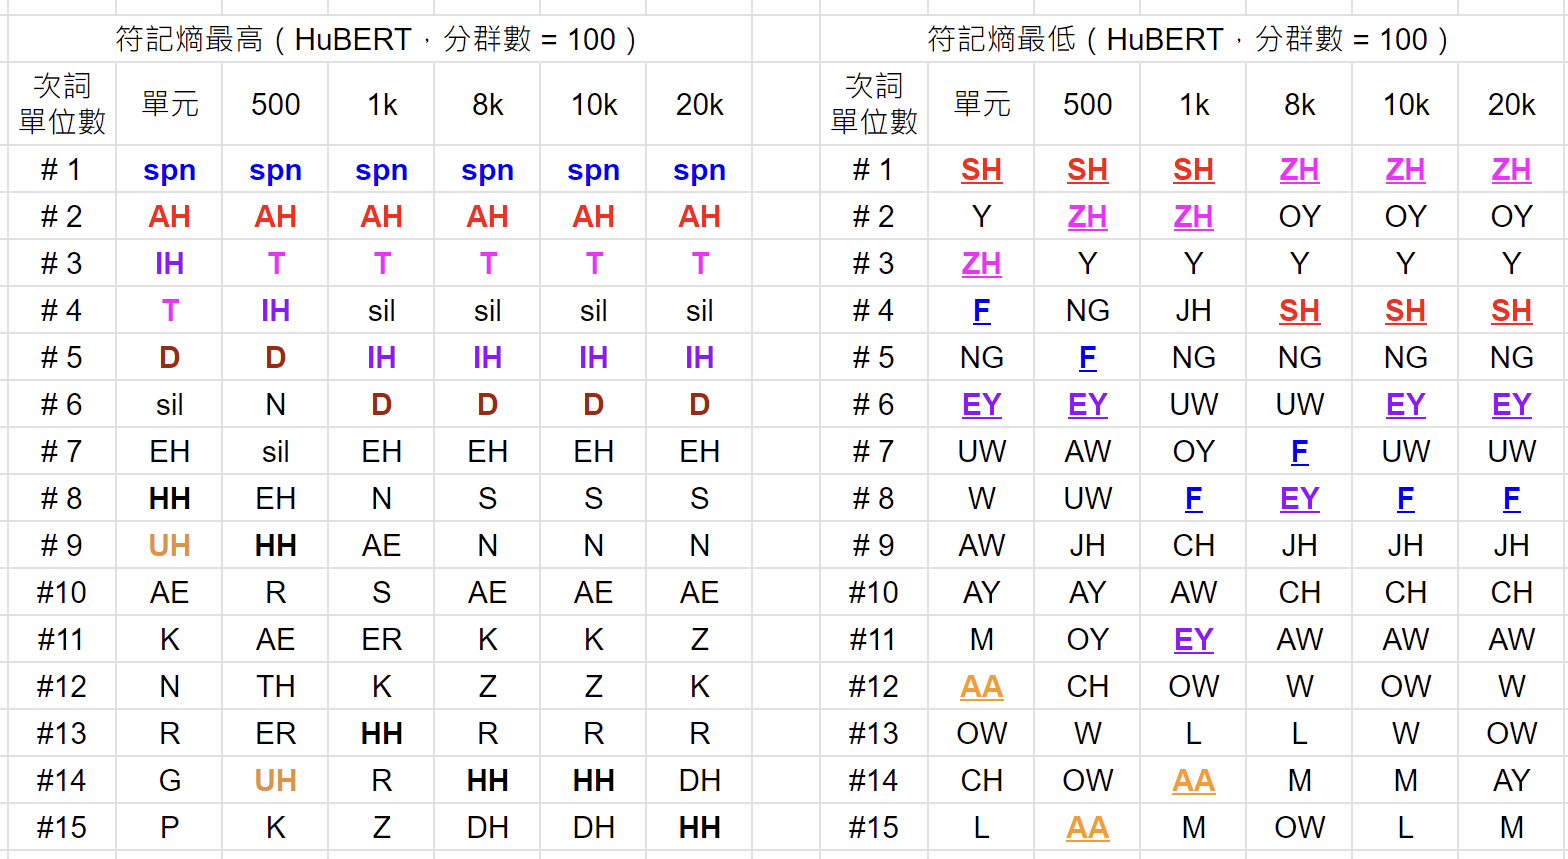
\includegraphics[width=\tempwidth]{figures/ch4figs/phnrank-hub100pcs.png}
                 \caption{分群數 = 100}
                 \label{fig:hub-u050-phnrank-hub100pcs}
             \end{subfigure}

             \caption{HuBERT 表徵、K-平均演算法分群數 50 和 100,}
             比較不同次詞單位種數時,符記熵最高與最低的音位排名
                         \label{fig:hub-u050-phnrank}
        \end{figure}
    }

    
  考慮完聲學片段,接著我們一樣以音位的角度切入,觀察各自音位的符記分佈集中程度。圖 \ref{fig:hub-u050-phnrank} 是對 HuBERT 模型所得的離散單元(比較分群數 50 和 100),以不同次詞單位種數
取得聲學片段後,
對應符記熵 $H(z|y)$ 最高與最低的排名。
比對最左側直行顯示的離散單元排名,亦即第三章不引入次詞單位的結果,可以發現整體排名趨勢雖有些微變動,但對應符記最分散的音位仍以 AH、IH、T、D 為主,而最集中的亦仍然是 ZH、SH、F、EY,與上一章的觀察接近。由此可以推論,音位本身的較容易或較難以歸類的特性,在對語音表徵進行分群時就已經大致呈現;然而,即便聲學片段的演算法允許將代表不同類別音位的離散單元重新組合成新的符記,卻仍舊維持了音位本身分散程度的趨勢。
因此,音位本身對應符記,不論是使用 K-平均演算法離散化獲得,或是以次詞單位重新歸類,這個分散程度的趨勢都是差不多的,音位本身的發音特徵確實是超出單一音框、影響範圍更廣的特性。 




{
\begin{figure}  % 有辦法再改圖
    \centering
    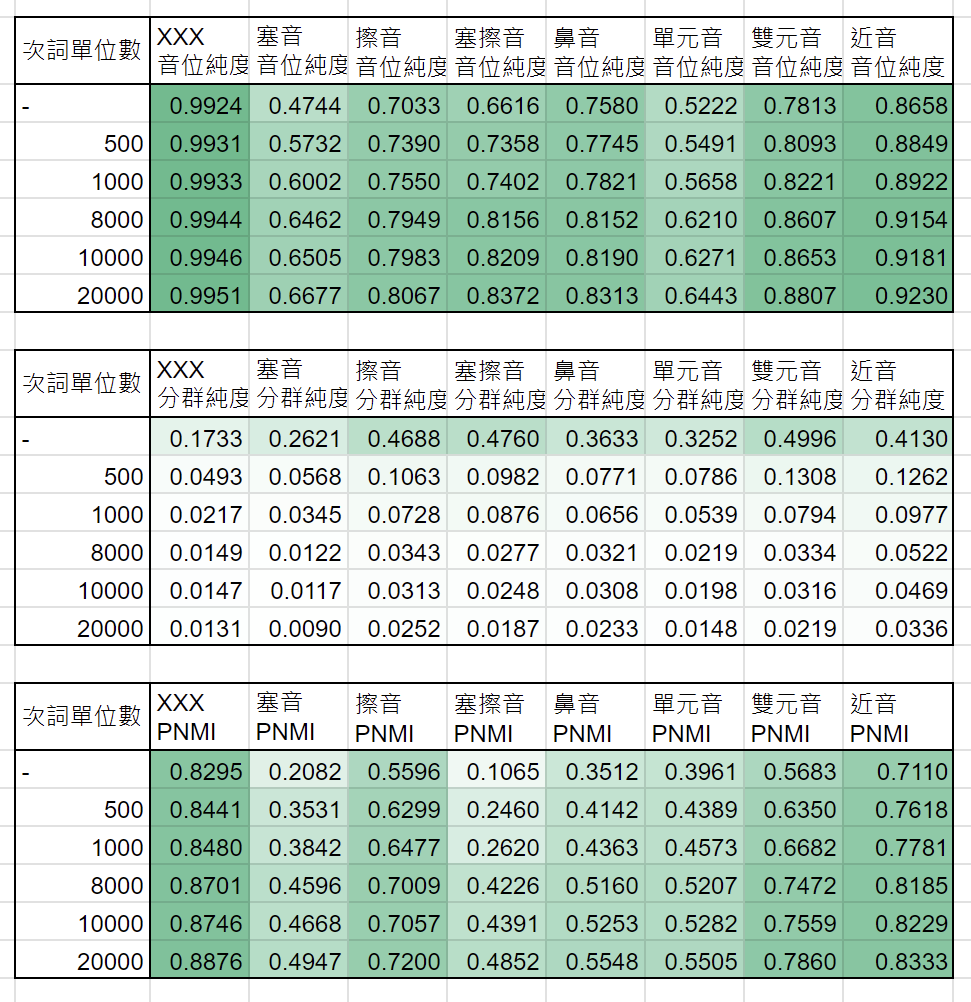
\includegraphics[width=0.6\linewidth]{figures/ch4figs/hub50-ap-detailedpur.png}
    \caption{HuBERT 分群數 50 的離散單元,以不同符記種數取得聲學片段後,}
    按照音位分類分開各自計算的純度與相互資訊
    \label{fig:hub50-ap-detailedpur}
\end{figure}
}


\begin{figure}
    \centering
    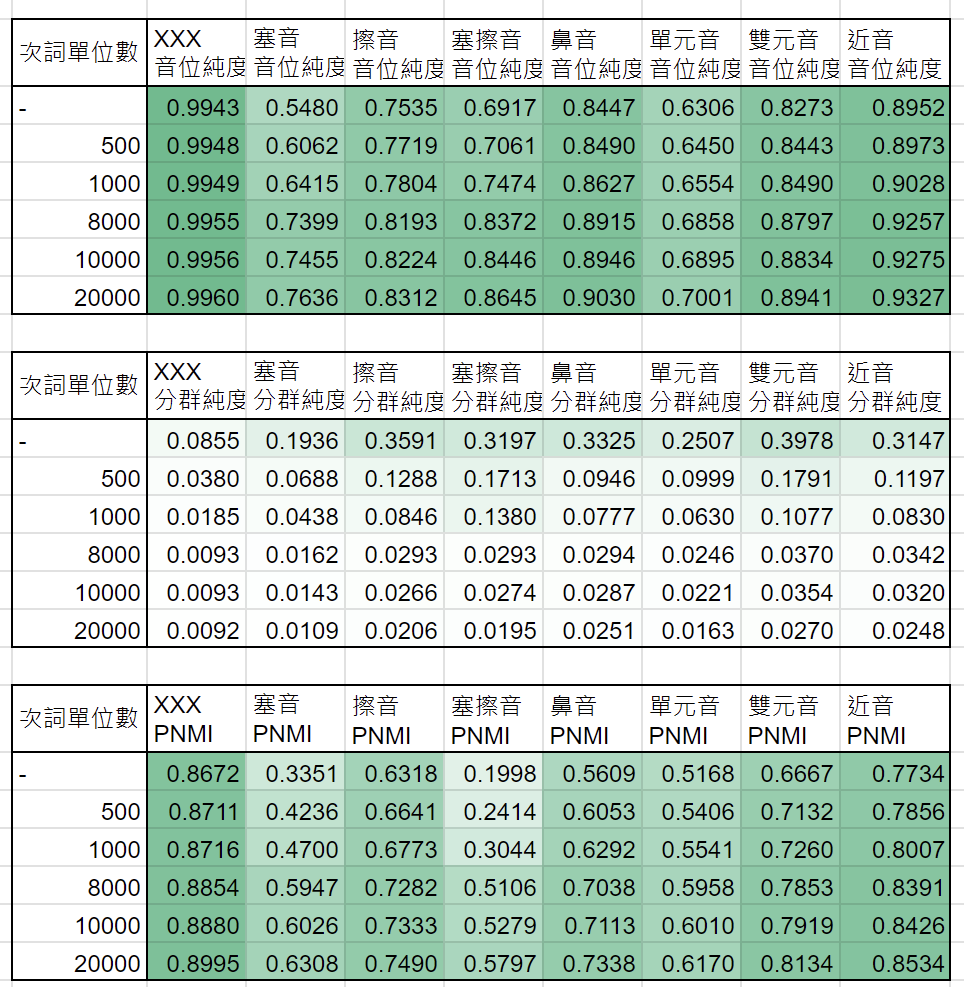
\includegraphics[width=0.6\linewidth]{figures/ch4figs/hub100-ap-detailedpur.png}
     \caption{HuBERT 分群數 100 的離散單元,以不同符記種數取得聲學片段後,}
    按照音位分類分開各自計算的純度與相互資訊
    \label{fig:hub100-ap-detailedpur}
\end{figure}


  
        最後,我們可以將音位分類分別考慮,統計其各自的純度與相互資訊數據,與上一章節比對。對 HuBERT 分群數 50 離散單元文本以不同次詞單位種數處理後,不同音位分類各自的純度與相互資訊數據以圖 \ref{fig:hub50-ap-detailedpur} 呈現。由結果可以發現,隨著次詞單位種數的增加,除了原本音位純度較低的塞音在音位純度與相互資訊的提升較為明顯外,其他音位分類的音位純度與相互資訊就已經較高,因而
雖然增加得不是很明顯,
但整體大致仍然有所改善。比較圖 \ref{fig:hub100-ap-detailedpur},可以確認此一變化在分群數改為 100 時依然可見。


% {

% \begin{figure}
%     \centering
%     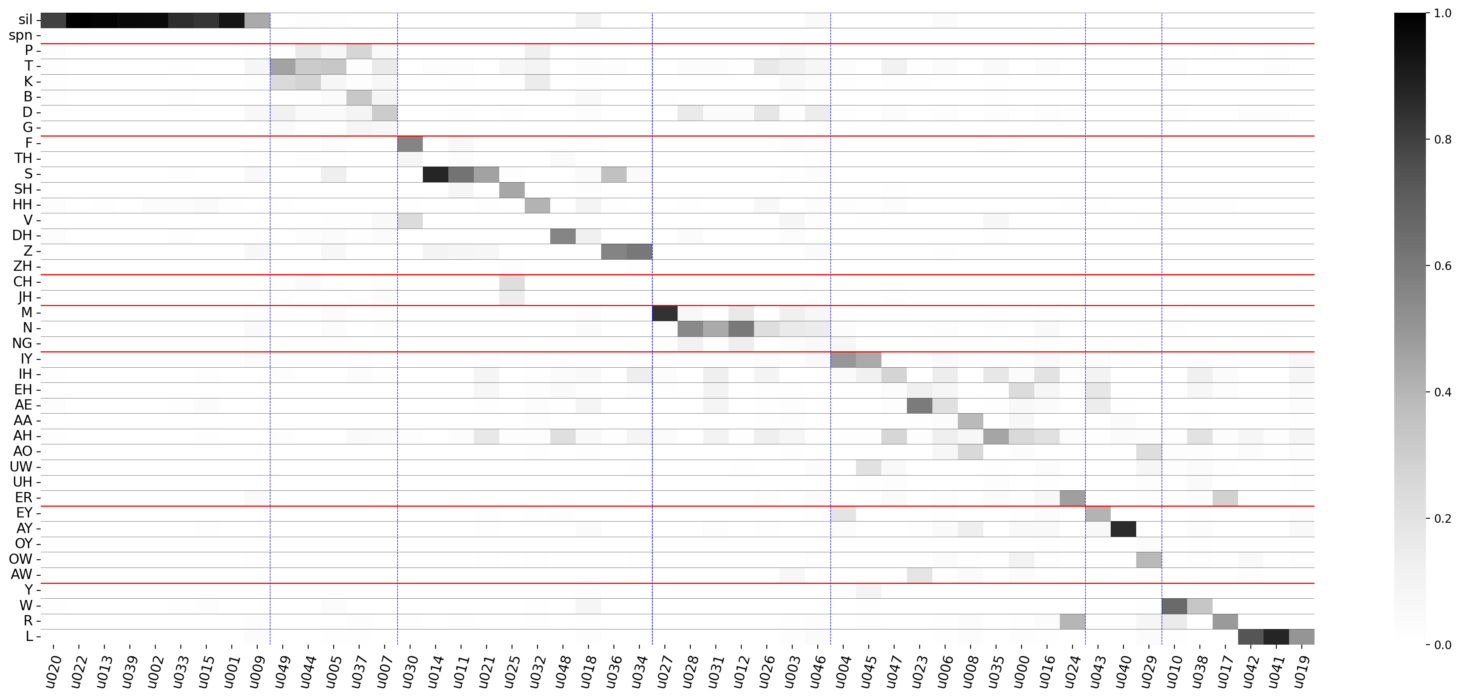
\includegraphics[width=1\linewidth]{figures/ch4figs/hub-u050-ap0000-givenunit-byphn.png}
%     \caption{hub-u050-ap0000-givenunit-byphn}
%     \label{fig:hub-u050-ap0000-givenunit-byphn--detailed}
% \end{figure}

% \begin{figure}
%     \centering
%     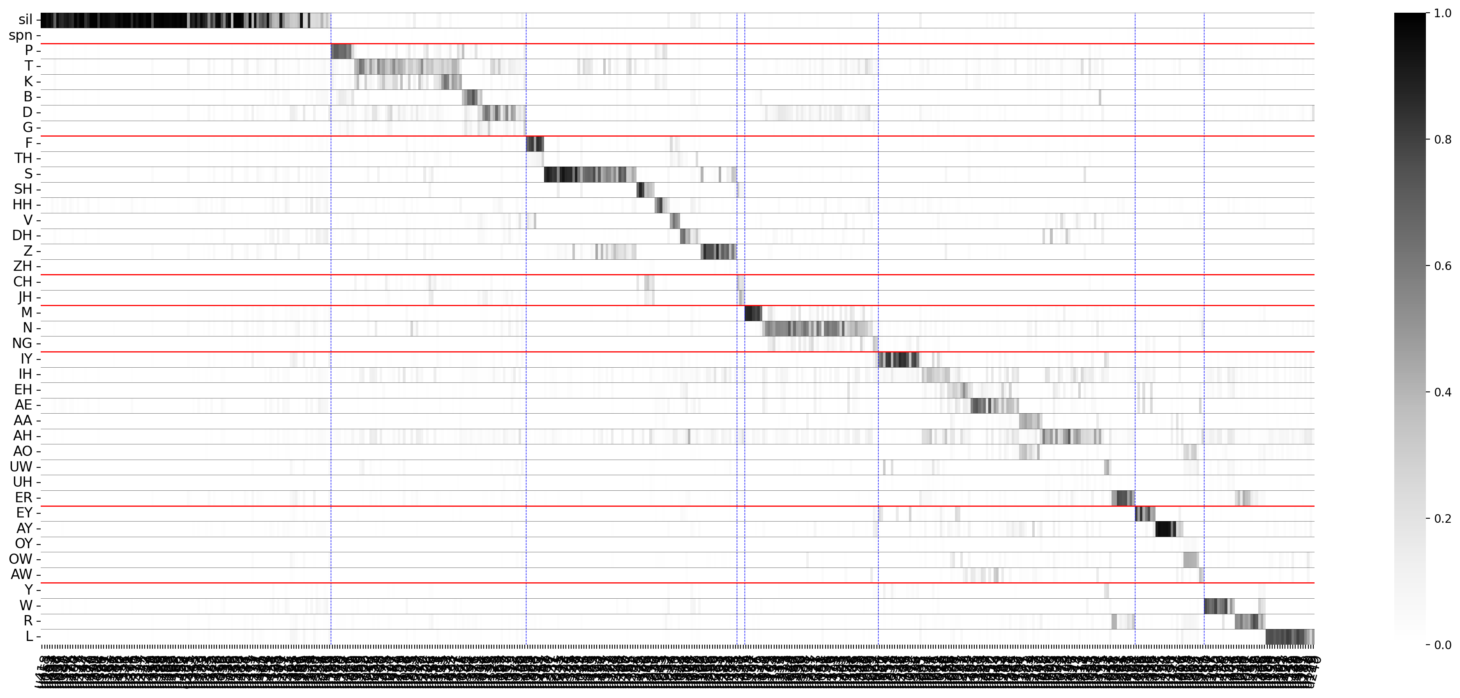
\includegraphics[width=1\linewidth]{figures/ch4figs/hub-u050-ap0500-givenunit-byphn.png}
%     \caption{hub-u050-ap0500-givenunit-byphn}
%     \label{fig:hub-u050-ap0500-givenunit-byphn--detailed}
% \end{figure}

% \begin{figure}
%     \centering
%     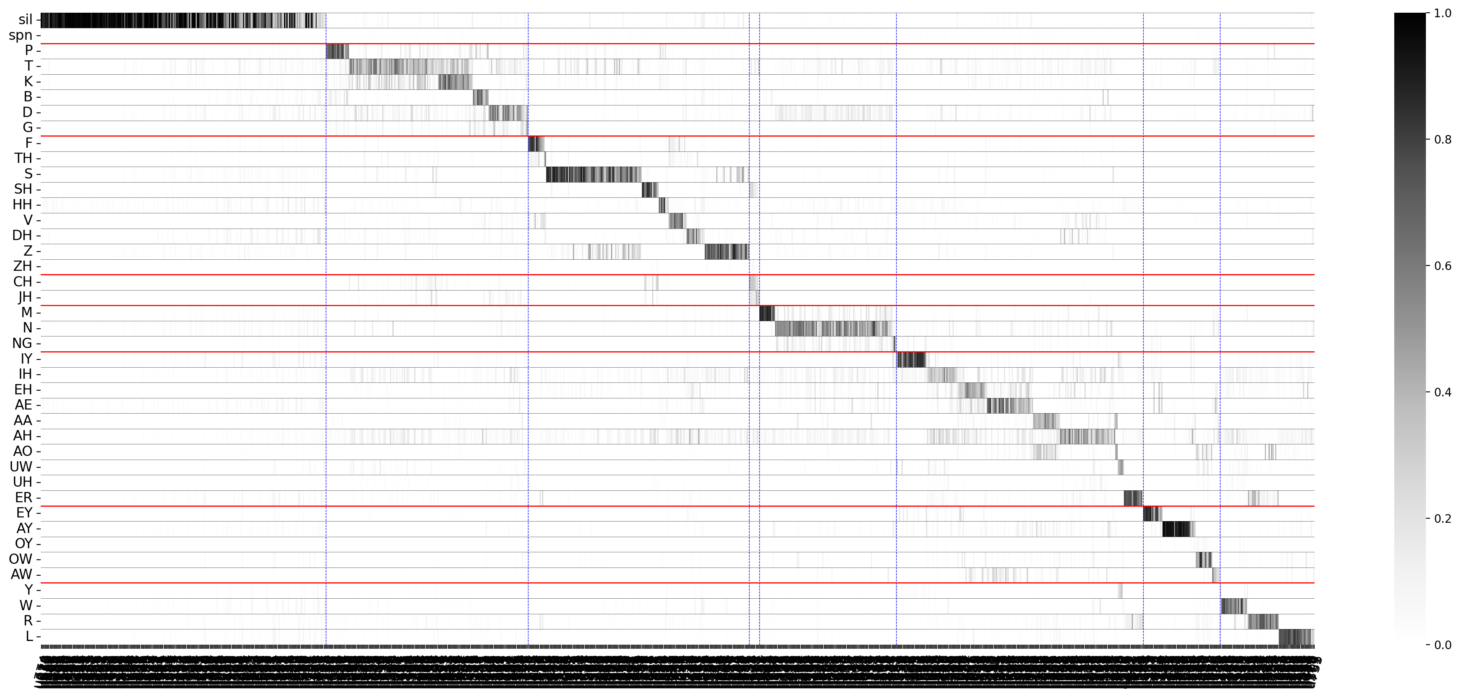
\includegraphics[width=1\linewidth]{figures/ch4figs/hub-u050-ap1000-givenunit-byphn.png}
%     \caption{hub-u050-ap1000-givenunit-byphn}
%     \label{fig:hub-u050-ap1000-givenunit-byphn--detailed}
% \end{figure}

% \begin{figure}
%     \centering
%     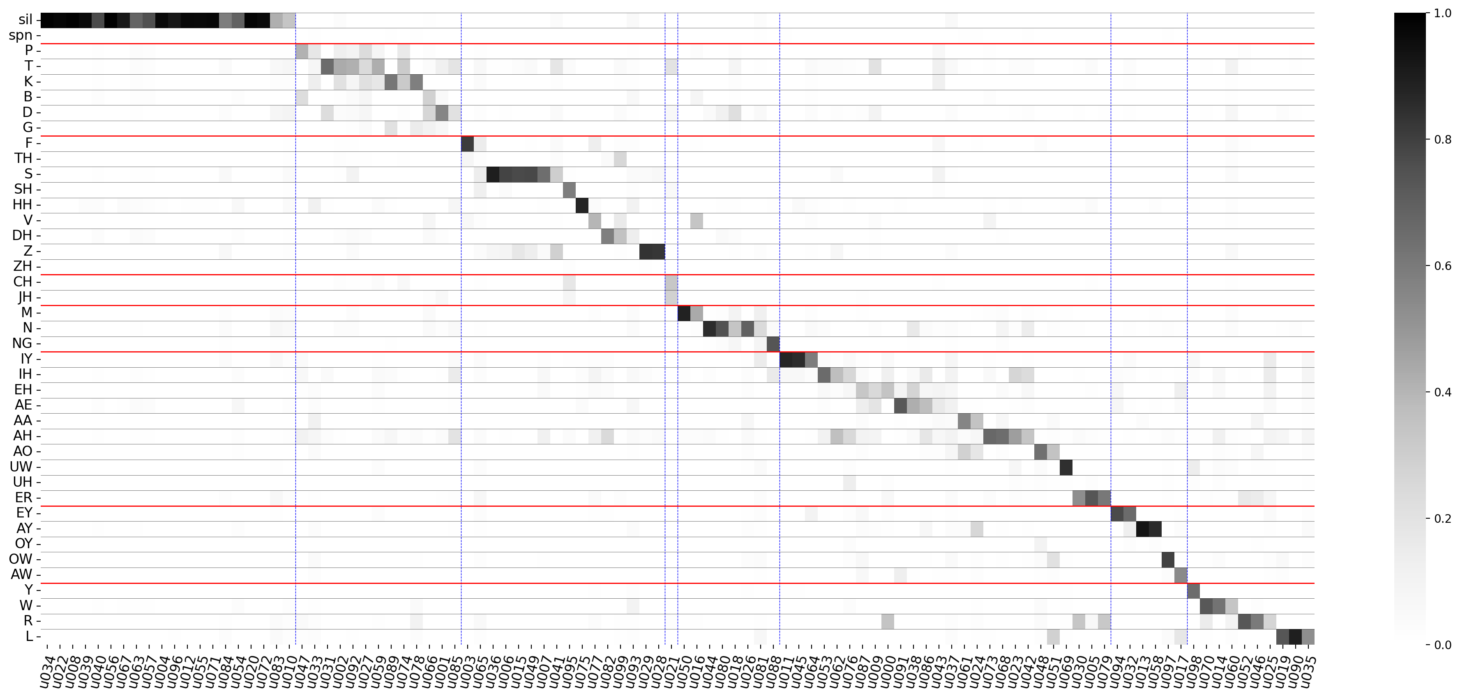
\includegraphics[width=1\linewidth]{figures/ch4figs/hub-u100-ap0000-givenunit-byphn.png}
%     \caption{hub-u100-ap0000-givenunit-byphn}
%     \label{fig:hub-u100-ap0000-givenunit-byphn--detailed}
% \end{figure}
% \begin{figure}
%     \centering
%     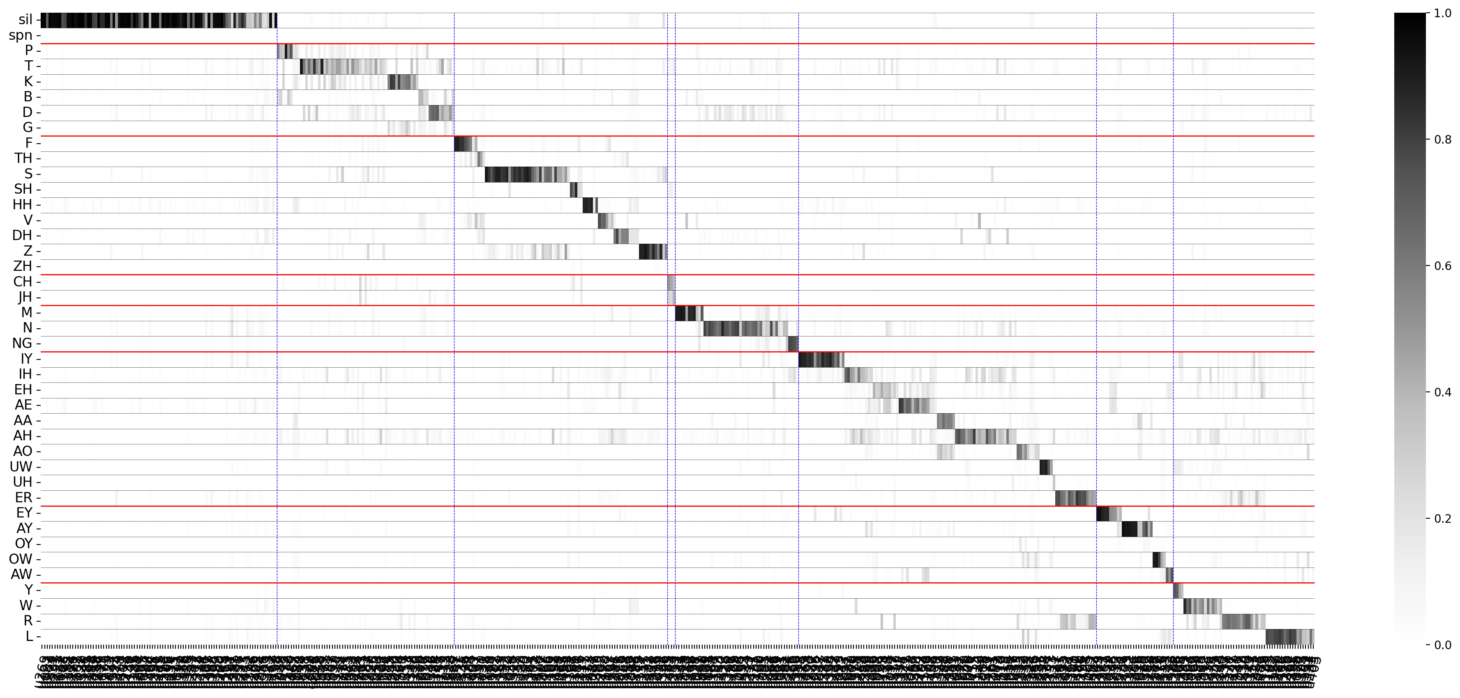
\includegraphics[width=1\linewidth]{figures/ch4figs/hub-u100-ap0500-givenunit-byphn.png}
%     \caption{hub-u100-ap0500-givenunit-byphn}
%     \label{fig:hub-u100-ap0500-givenunit-byphn--detailed}
% \end{figure}
% \begin{figure}
%     \centering
%     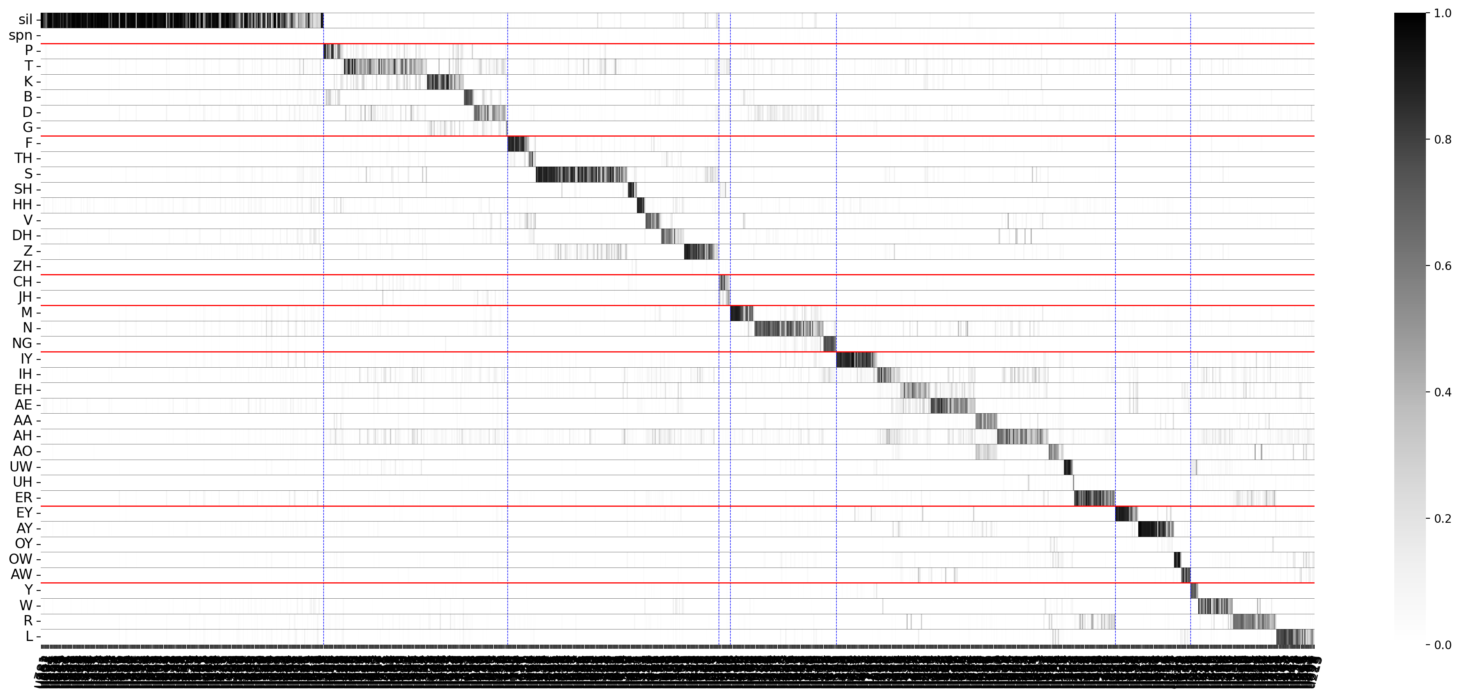
\includegraphics[width=1\linewidth]{figures/ch4figs/hub-u100-ap1000-givenunit-byphn.png}
%     \caption{hub-u100-ap1000-givenunit-byphn}
%     \label{fig:hub-u100-ap1000-givenunit-byphn--detailed}
% \end{figure}
% }  % heatmaps


\jcm{section{分析結果} }
\jcm{  以下數據中的「長度壓縮比率」係指透過分詞方法後,每一個句子的「單詞」數與原先離散單元的數量相比之比值。由於長度壓縮比率是針對離散單元分詞所得到,與標註無關,因此只在音位分析的表格上呈現。}
\jcm{subsection{基於各自音位的分析}}
\jcm{  首先,為了比較不同詞表大小對於純度、相互資訊等數據的影響,先分別固定語音模型為 HuBERT 和 Wav2vec 2.0,在離散單元的分群數量為 50、100、200 三種設定下,觀察詞表大小造成的變化。由 HuBERT (表 \ref{tab:hubert-phn-results-})和 Wav2vec 2.0(表 \ref{tab:w2v2-phn-results})的數據比較可觀察到,詞表大小上升除了使得音位純度提高以外,相互資訊也是隨之提高的,可以發現使用分詞方法並給予足夠大的詞表,對於找出語音中的資訊確實有所幫助。}
\jcm{        接著從另一個角度切入,比較同樣都是離散單元分群數為 200 的條件下,不同語音基石模型的分析數據。由表 \ref{tab:ch4-models-phn} 可以發現,HuBERT 模型在音位純度與相互資訊勝過其他模型,這個結論與上一章節是一致的。}
\jcm{        有趣的是,觀察長度壓縮比率可以發現,CPC 模型在分詞演算法的引入後,能夠使序列變得最短,但同時在音位純度與相互資訊上也有所犧牲;而 HuBERT 雖然在這些分析數據上高過其他三者,卻同時達成了比 Wav2vec 2.0 和 LogMel 更好的壓縮比率。因此綜合看來,這很可能是目前使用語音離散單元進行研究時,HuBERT 模型仍然是領域內首選的緣由。}
\jcm{                \input{tables/chapter4/chapter4-5.ztable1-1.tex}
\input{tables/chapter4/chapter4-5.ztable1-2.tex}
\input{tables/chapter4/chapter4-5.ztable1-3.tex}}
\jcm{subsection{基於語音學分類的分析}}
\jcm{  最後觀察將語音標註換成語音學分類的結果,一樣可以從表 \ref{tab:hubert-pcls-results}、\ref{tab:w2v2-pcls-results} 和 \ref{tab:ch4-models-pcls} 觀察到與上一小節相同的趨勢。}
\jcm{                
        \begin{table}[!htbp]
            \centering
            \begin{subtable}[t]{\textwidth}
                \centering
                \begin{tabular}{|c|c|c|c|c|c|} \hline 
                        詞表大小  & 標註純度 & 分群純度 & 標註熵 & 離散單元熵 &     NMI   \\ \hline 
                       50 (未分詞)&   0.7466  &  0.1422 & 1.7530 &   3.8681 &  0.5742 \\ \hline 
                           500    &  0.7510  &  0.0345  & 1.7530 &  6.0282  &     0.5789  \\ \hline 
                          1000    &  0.7492  &  0.0225  & 1.7530 &  6.6594  &     0.5756  \\ \hline 
                          8000    &  0.7288  &  0.0116  & 1.7530 &  8.5192  &     0.5630  \\ \hline 
                         10000    &  0.7248  &  0.0110  & 1.7530 &  8.7207  &     0.5606  \\ \hline 
                         20000    &  0.7109  &  0.0089  & 1.7530 &  9.3527  &     0.5537  \\ \hline 
                \end{tabular}
\caption{群數 = 50}
                \label{tab:ch4-hubert-pcls-clu050}
            \end{subtable}        

            \jefftablesep        

            \begin{subtable}[t]{\textwidth}
                \centering
                \begin{tabular}{|c|c|c|c|c|c|} \hline 
                        詞表大小  & 標註純度 & 分群純度 & 標註熵 & 離散單元熵 &     NMI   \\ \hline 
 100 (未分詞)&              0.7804 &   0.0856 &         1.7530 &     4.5704 &  0.6148\\ \hline 
                           500    &  0.7787  &  0.0300  & 1.7530 &  6.0655  &     0.6178  \\ \hline 
                          1000    &  0.7751  &  0.0210  & 1.7530 &  6.7181  &     0.6176  \\ \hline 
                          8000    &  0.7507  &  0.0095  & 1.7530 &  8.5954  &     0.6030  \\ \hline 
                         10000    &  0.7468  &  0.0087  & 1.7530 &  8.7938  &     0.6008  \\ \hline 
                         20000    &  0.7347  &  0.0072  & 1.7530 &  9.4123  &     0.5943  \\ \hline 
                \end{tabular}
\caption{群數 = 100}
                \label{tab:ch4-hubert-pcls-clu100}
            \end{subtable}        

            \jefftablesep        

            \begin{subtable}[t]{\textwidth}
                \centering
                \begin{tabular}{|c|c|c|c|c|c|} \hline 
                        詞表大小  & 標註純度 & 分群純度 & 標註熵 & 離散單元熵 &     NMI   \\ \hline 
 200 (未分詞)&              0.8004 &   0.0464 &         1.7530 &     5.2681 &  0.6563\\ \hline 
                           500    &  0.7875  &  0.0269  & 1.7530 &  6.0986  &     0.6469  \\ \hline 
                          1000    &  0.7788  &  0.0170  & 1.7530 &  6.7786  &     0.6385  \\ \hline 
                          8000    &  0.7625  &  0.0071  & 1.7530 &  8.6544  &     0.6266  \\ \hline 
                         10000    &  0.7601  &  0.0064  & 1.7530 &  8.8535  &     0.6251  \\ \hline 
                         20000    &  0.7514  &  0.0051  & 1.7530 &  9.4737  &     0.6200   \\ \hline
                \end{tabular}
\caption{群數 = 200}
                \label{tab:ch4-hubert-pcls-clu200}
            \end{subtable}        

\caption{HuBERT 模型在不同詞表大小時的語音學類別分析數據}
            \label{tab:hubert-pcls-results}
        \end{table}

\begin{table}[!htbp]
    \centering
    \begin{subtable}[t]{\textwidth}
        \centering
        \begin{tabular}{|c|c|c|c|c|c|} \hline 
                詞表大小 & 標註純度 & 分群純度 & 標註熵 & 離散單元熵 &     NMI \\ \hline 
 50 (未分詞)&      0.6913 &   0.1570 &         1.7530 &     3.8215 &  0.4682\\ \hline 
                  500  &  0.7018 &    0.0339 &   1.7530 &   6.0328 &       0.4873  \\ \hline 
                 1000  &  0.7058 &    0.0273 &   1.7530 &   6.6250 &       0.4913  \\ \hline 
                 8000  &  0.7041 &    0.0158 &   1.7530 &   8.4954 &       0.4956  \\ \hline 
                10000  &  0.7033 &    0.0152 &   1.7530 &   8.6966 &       0.4963  \\ \hline 
                20000  &  0.6961 &    0.0128 &   1.7530 &   9.3471 &       0.4954  \\ \hline 
        \end{tabular}
\caption{群數 = 50}
        \label{tab:ch4-w2v2-pcls-clu050}
    \end{subtable}        

    \jefftablesep        

    \begin{subtable}[t]{\textwidth}
        \centering
        \begin{tabular}{|c|c|c|c|c|c|} \hline 
                詞表大小 & 標註純度 & 分群純度 & 標註熵 & 離散單元熵 &     NMI \\ \hline 
 100 (未分詞)&     0.7219 &   0.0889 &         1.7530 &     4.5284 &  0.5252 \\ \hline 
                  500  &  0.7142 &    0.0288 &   1.7530 &   6.0769 &       0.5297  \\ \hline 
                 1000  &  0.7132 &    0.0197 &   1.7530 &   6.7265 &       0.5294  \\ \hline 
                 8000  &  0.7173 &    0.0108 &   1.7530 &   8.5576 &       0.5352  \\ \hline 
                10000  &  0.7171 &    0.0105 &   1.7530 &   8.7602 &       0.5360  \\ \hline 
                20000  &  0.7149 &    0.0089 &   1.7530 &   9.4070 &       0.5379  \\ \hline 
        \end{tabular}
\caption{群數 = 100}
        \label{tab:ch4-w2v2-pcls-clu100}
    \end{subtable}        

    \jefftablesep        

    \begin{subtable}[t]{\textwidth}
        \centering
        \begin{tabular}{|c|c|c|c|c|c|} \hline 
                詞表大小 & 標註純度 & 分群純度 & 標註熵 & 離散單元熵 &     NMI \\ \hline 
  200 (未分詞)&     0.7490 &   0.0527 &         1.7530 &     5.2173 &  0.5671  \\ \hline 
                  500  &  0.7465 &    0.0310 &   1.7530 &   6.0756 &       0.5685  \\ \hline 
                 1000  &  0.7451 &    0.0199 &   1.7530 &   6.7483 &       0.5692  \\ \hline 
                 8000  &  0.7405 &    0.0071 &   1.7530 &   8.6065 &       0.5725  \\ \hline 
                10000  &  0.7399 &    0.0066 &   1.7530 &   8.8136 &       0.5729  \\ \hline 
                20000  &  0.7391 &    0.0055 &   1.7530 &   9.4561 &       0.5757   \\ \hline
        \end{tabular}
\caption{群數 = 200}
        \label{tab:ch4-w2v2-pcls-clu200}
    \end{subtable}        

\caption{Wav2vec 2.0 模型在不同詞表大小時的語音學類別分析數據}
    \label{tab:w2v2-pcls-results}
\end{table}


        \begin{table}[!htbp]
            \centering
            \begin{subtable}[t]{\textwidth}
                \centering
                \begin{tabular}{|c|c|c|c|c|c|} \hline 
                        詞表大小  & 標註純度 & 分群純度 & 標註熵 & 離散單元熵 &     NMI  \\ \hline 
  200 (未分詞)&         0.8004 &   0.0464 &         1.7530 &     5.2681 &  0.6563\\ \hline 
                            500 &  0.7875 &    0.0269 &   1.7530   & 6.0986 &    0.6469 \\ \hline %%   2.0934
                           1000 &  0.7788 &    0.0170 &   1.7530   & 6.7786 &    0.6385 \\ \hline %%   2.1156
                          10000 &  0.7601 &    0.0064 &   1.7530   & 8.8535 &    0.6251 \\ \hline %%   2.1826
                \end{tabular}
\caption{HuBERT}
                \label{tab:ch4-pcls-model-hubert}
            \end{subtable}        

            \jefftablesep        

            \begin{subtable}[t]{\textwidth}
                \centering
                \begin{tabular}{|c|c|c|c|c|c|} \hline 
                        詞表大小  & 標註純度 & 分群純度 & 標註熵 & 離散單元熵 &     NMI  \\ \hline 
  200 (未分詞)&         0.7490 &   0.0527 &         1.7530 &     5.2173 &  0.5671 \\ \hline 
                            500 &  0.7465 &    0.0310 &   1.7530   & 6.0756 &    0.5685 \\ \hline %%   1.7491
                           1000 &  0.7451 &    0.0199 &   1.7530   & 6.7483 &    0.5692 \\ \hline %%   1.7727
                          10000 &  0.7399 &    0.0066 &   1.7530   & 8.8136 &    0.5729 \\ \hline %%   1.8791
                \end{tabular}
\caption{Wav2vec 2.0}
                \label{tab:ch4-pcls-model-w2v2}
            \end{subtable}        

            
            \jefftablesep        

            \begin{subtable}[t]{\textwidth}
                \centering
                \begin{tabular}{|c|c|c|c|c|c|} \hline 
                        詞表大小  & 標註純度 & 分群純度 & 標註熵 & 離散單元熵 &     NMI  \\ \hline 
 200 (未分詞)&         0.7947 &   0.0644 &         1.7530 &     5.1885 &  0.6345 \\ \hline 
                            500 &  0.7925 &    0.0369 &   1.7530   & 6.0343 &    0.6368 \\ \hline %%   1.9677
                           1000 &  0.7882 &    0.0223 &   1.7530   & 6.7245 &    0.6349 \\ \hline %%   1.9818
                          10000 &  0.7609 &    0.0096 &   1.7530   & 8.8593 &    0.6175 \\ \hline %%   2.0277
                \end{tabular}
\caption{CPC}
                \label{tab:ch4-pcls-model-cpc}
            \end{subtable}        

            \jefftablesep        

            \begin{subtable}[t]{\textwidth}
                \centering
                \begin{tabular}{|c|c|c|c|c|c|} \hline 
                詞表大小 & 標註純度 & 分群純度 & 標註熵 & 離散單元熵 &     NMI \\ \hline 
  200 (未分詞)&         0.6107 &   0.0335 &         1.7530 &     5.2322 &  0.3652 \\ \hline 
                            500 &  0.6156 &    0.0247 &   1.7530   & 6.1035 &    0.3801 \\ \hline %%   1.0166
                           1000 &  0.6189 &    0.0137 &   1.7530   & 6.7602 &    0.3875 \\ \hline %%   1.0376
                          10000 &  0.6322 &    0.0096 &   1.7530   & 8.7579 &    0.4085 \\ \hline %%   1.1211
                \end{tabular}
\caption{LogMel}
                \label{tab:ch4-pcls-model-logmel}
            \end{subtable}        

\caption{固定離散單元群數皆為 200,不同基石模型的語音學類別分析數據}
            \label{tab:ch4-models-pcls}
        \end{table}
        
}

\subsection{分析結論}

  藉由改以次詞單位重新組合離散單元得到聲學片段,
% 我們可以發現
% 可以
透過符記種類數量的提升,
聲學片段可以區別出語音訊號中更細節的語音差異,
進而得以提升音位純度與相互資訊等數據,
提高符記與音位之間的相關性。
同時,
次詞單位的特性雖然允許
對應到不同音位的離散單元重新組合,
然而如此產生的新符記
,
每個音位對應符記的集中或分散程度卻
% 卻在對應的音位分佈卻
% 不太有
差異不大。
因此,
透過將次詞單位應用在離散單元的嘗試,
結合多個離散單元重新編碼語音訊號,
聲學片段在捕捉語音訊號規律上,
儘管效果不如直接對語音表徵進行分群的離散單元好,
卻能作為需要探索更細微語音資訊差異時,
除了 K-平均演算法之外對語音訊號離散化的另一個選擇。
% ???? (delete length)

% 在序列長度相對縮短的前提下,音位的純度卻也獲得了提升,足以證明分詞演算法的引入,可以幫助離散單元考量多於一個音框的語音資訊,建構於精細的音框之上,找出更接近人類解讀語音最小單位資訊。期望以此發現,可以使得語音語言模型建立時,模型在處理語音語料庫時,能夠以更接近文字的序列長度與資訊進行訓練,獲得更接近文字模型的效果。

% 1. piece 可以 encode 更細節的資訊
% 2. 但 cls 降了
% 3. 對應的發音特性大致不變

\section{本章總結}
  本章節首先
介紹了文字處理中常用的次詞單位,並嘗試對離散單元序列重新組合成聲學片段。接著,仿照第三章的分析方式,將離散單元與聲學片段互相比較,對比兩種不同符記與音位間對應關係的變化。結果顯示,無論是使用離散單元或次詞單位,儘管兩種方式在語音資訊捕捉效果上有所不同,但隨著符記種類的增加,都能獲得更加細節的語音資訊,並提升與音位之間的相關性。
% 期望此一發現,可以在未來要以符記建立語音語言模型時,除了 K-平均演算法的離散單元以外,考慮與次詞單位的演算法配合使用,以更細緻全面的從語音訊號中,找出和音位等的語音學資訊最相關的資訊。
期望這一發現可以在未來建立語音語言模型時,除了 K-平均演算法的離散單元外,考慮與次詞單位的演算法結合使用,以更全面和細緻的從語音訊號中提取與音位相關的語音學資訊。  % 以  token? 

% \chapter{結論與展望}

\section{研究貢獻與討論}
  
本論文的主旨,在於分析語音基石模型的離散表徵,與語音標註之間的純度和相互資訊等數據的相關性,並且透過分詞方法的引入,嘗試將多個離散單元進行結合後,觀察學習到的新符記是否和音位等標註更加一致。 

首先,論文第三章介紹了與無文字架構以及語音表徵相關的分析研究,隨後簡介語音學知識中,對於不同音位之間如何按照發音特性分門別類。有了音位與語音學分類兩種語音標註後,借鑑 HuBERT 提及的純度和相互資訊的分析方式,對離散表徵與語音標註之間,兩者的相關性進行分析與觀察,比對無文字架構中不同語音離散表徵的統計特性。結果可發現,HuBERT 作為目前無文字架構最常用的語音離散表徵模型的理由,很可能來自於它們的音位純度與相互資訊都相對較高,因而更能捕捉到語音中與內容相關的重要資訊,且同樣的趨勢在語音學分類的標註也可以被觀察到。

其後在論文第四章,考慮到音位與離散單元往往是一對多的關係,
藉著嘗試引入自然語言處理常用的分詞方法,
重新對離散單元的序列進行分組,並且比較不同詞表大小對這些分析數據的影響。
考量語音不如英語的文字系統具備明確的空格提示,
本研究採取單一詞作為分詞方法進行
實驗,
並比較不同模型與不同詞表大小對第三章的分析數據是否造成影響。

結果顯示,
藉助加入分詞方法並提供足夠大的詞表,確實能夠讓不同音位的純度以及相互資訊有所提升,
讓多個離散單元之間有機會相互結合、重新分組,更能捕捉語音訊號中的內容資訊。
且在四種語音表徵之間,HuBERT 依然是所有模型中音位純度和相互資訊最高者,還達成了一定的序列長度壓縮比率,相較之下 CPC 模型雖然壓縮比率更低,卻犧牲掉過多語音資訊導致相關數據反而較差。這也解釋了為什麼目前在離散單元相關的研究中,無論是使用單一離散單元,或是使用分詞方法進行長度壓縮等,HuBERT 都仍是最有利於後續語音任務的訓練與應用的模型。

 

\section{未來展望}
  
希望這些對離散單元與分詞方法應用的嘗試,能幫助我們在訓練任務之前,決定哪種語音基石模型更適合作為離散編碼語音訊號的基礎。接下來,我們期望能針對常見的語音任務,特別是語音辨識和語音翻譯等內容處理相關的任務,比對離散單元促成的實際成效和分析數據之間的關係,並對這些任務中的錯誤案例進行統計和個案探討。

另外,對於如何結合語音離散單元,除了將其視為文字進行分詞演算法外,我們還可以使用其他方式對離散單元序列進行分組,以達成壓縮序列長度並使其與音位等語音內容更加一致的目標。例如,將此目標形塑為語音分段(Speech Segmentation)任務等,也是未來可以嘗試的離散單元分組方式。

最後,利用語音學分組的切入點,或許可以在未來分析離散單元或連續語音表徵時,不再僅限於參考音位或文字,還可以從語音學知識提供的相似性資訊出發,為錯誤發音修正等任務提供衡量的依據。


\chapter{結論與展望}

\section{研究貢獻與討論}

  本論文的主旨,在於分析語音基石模型的離散表徵,與語音標註之間的純度和相互資訊等數據的相關性,並且透過分詞方法的引入,嘗試將多個離散單元進行結合後,觀察學習到的新符記是否和音位等標註更加一致。 

        首先,論文第三章介紹了與無文字架構以及語音表徵相關的分析研究,隨後簡介語音學知識中,對於不同音位之間如何按照發音特性分門別類。有了音位與語音學分類兩種語音標註後,借鑑 HuBERT 提及的純度和相互資訊的分析方式,對離散表徵與語音標註之間,兩者的相關性進行分析與觀察,比對無文字架構中不同語音離散表徵的統計特性。結果可發現,HuBERT 作為目前無文字架構最常用的語音離散表徵模型的理由,很可能來自於它們的音位純度與相互資訊都相對較高,因而更能捕捉到語音中與內容相關的重要資訊,且同樣的趨勢在語音學分類的標註也可以被觀察到。

        其後在論文第四章,考慮到音位與離散單元往往是一對多的關係,藉著嘗試引入自然語言處理常用的分詞方法,重新對離散單元的序列進行分組,並且比較不同詞表大小對這些分析數據的影響。考量語音不如英語的文字系統具備明確的空格提示,本研究採取單一詞作為分詞方法進行實驗,並比較不同模型與不同詞表大小對第三章的分析數據是否造成影響。

        結果顯示,藉助加入分詞方法並提供足夠大的詞表,確實能夠讓不同音位的純度以及相互資訊有所提升,讓多個離散單元之間有機會相互結合、重新分組,更能捕捉語音訊號中的內容資訊。且在四種語音表徵之間,HuBERT 依然是所有模型中音位純度和相互資訊最高者,還達成了一定的序列長度壓縮比率,相較之下 CPC 模型雖然壓縮比率更低,卻犧牲掉過多語音資訊導致相關數據反而較差。這也解釋了為什麼目前在離散單元相關的研究中,無論是使用單一離散單元,或是使用分詞方法進行長度壓縮等,HuBERT 都仍是最有利於後續語音任務的訓練與應用的模型。

\section{未來展望}

  希望這些對離散單元與分詞方法應用的嘗試,能幫助我們在訓練任務之前,決定哪種語音基石模型更適合作為離散編碼語音訊號的基礎。接下來,我們期望能針對常見的語音任務,特別是語音辨識和語音翻譯等內容處理相關的任務,比對離散單元促成的實際成效和分析數據之間的關係,並對這些任務中的錯誤案例進行統計和個案探討。

        另外,對於如何結合語音離散單元,除了將其視為文字進行分詞演算法外,我們還可以使用其他方式對離散單元序列進行分組,以達成壓縮序列長度並使其與音位等語音內容更加一致的目標。例如,將此目標形塑為語音分段(Speech Segmentation)任務等,也是未來可以嘗試的離散單元分組方式。

        最後,利用語音學分組的切入點,或許可以在未來分析離散單元或連續語音表徵時,不再僅限於參考音位或文字,還可以從語音學知識提供的相似性資訊出發,為錯誤發音修正等任務提供衡量的依據。

}

% \chapter{導論}

\section{研究動機}
  
語言是人與人彼此交流最主要的橋樑,而人們互相溝通最自然的方式便是透過說話的語音(Speech)達成。人類往往是自幼就牙牙學語開始說話,直到已屆學齡左右才開始學習認字與書寫。雖然在這個資訊爆炸的時代,人們已經習慣以文字呈現的語言作為獲取資訊的主要媒介,但不論如何,各種書寫系統其背後承載的語言必定有語音的形式作為對應。更何況世界上現存大約七千多種 \cite{eberhard_ethnologue_2024} 語言中,絕大多數不見得存在成熟且普及的文字系統,卻無礙於這些語言被人們所熟悉和使用。因此,「語音」作為語言不可或缺的存在方式,了解它和研究它的價值自然不言而喻。

然而,相對於穩定、易於處理和保存的文字文本,語音訊號的變化萬千,蘊藏了大量從語者風格、表達內容到抑揚頓挫(韻律,Prosody)等不同層次的訊息,使得對它的處理、研究相比之下複雜度與難度劇增。由於語音的這種特性,過往對於語言最有興趣的語言學家們,即便明白語音作為多數語言主體的事實,也不得不藉文字符號為依託進行探索。進入資訊化時代後,藉助電腦硬體等計算設備的幫助,從語料庫、計算語言學到自然語言處理等透過科技的力量發展語言處理技術的領域,頗長一段時間也是專注於文字的處理與分析。
而嘗試結合訊號處理發展的語音技術領域,當時則是透過語言學家對語言的領域知識,例如從音位(Phoneme)、構詞(Morphology)、語法(Syntax)等等用以刻劃人類語音和語言特性的概念,將之結合機器學習建立模型,開發技術以方便人們能以語音這種更靈活的媒介,更好的讓電腦、手機等科技工具可以更接近「直接溝通」的使用方式,便利人們的日常生活。

近年來,由於圖形處理器(Graphics Processing Unit,GPU)等硬體平行運算技術的進步,深層學習(Deep Learning)快速崛起成為人工智慧的主流,有了此項機器學習的技術,模型的彈性能夠更好的萃取資料、更貼近的尋找資料背後的機制並進行預測,使得人們不再非得依賴大量費時費工的人類標注過程,進而使得利用大量語料庫發展語言技術,進一步推進語言科技發展成為可能。尤其在自監督學習(Self-supervised Learning)技術出現之後,深層學習模型可以依照人們給定的方向,更細緻的從大量未標注、相較容易取得的語音或文字的語料,找出其中的語音、語法及語義等等結構,形成帶有對人類語言有前所未見表現的基石模型(Foundation Model),是這個領域的一大里程碑。尤其在以處理文字為主體的自然語言處理領域,甚至出現了幾乎使人類真偽難辨的生成式模型,改變了人們生活的方方面面。

借鏡文字方面的成功經驗,語音處理領域的研究者們也開始嘗試將語言模型(Language Model)的概念套用於變化莫測的語音訊號之上,原先人們藉助訊號處理知識一直使用的各種語音訊號特徵(Feature)也在自監督學習的架構之下,出現了許多模型從大量語音資料中得到的「語音表徵(Speech Representation)」,作為精煉語音資訊的另外一種新選擇開始廣泛被採用。然而,相比於文字符號的穩定與單純,語音的複雜性使得它處理起來會需要更大量的資料和運算資源來擷取其中不同層次的細節,而且作為物理訊號,語音還必須處理掉環境中的雜訊等干擾。為了從紛亂的聲音中提取出最重要的訊息,向量量化(Vector Quantization)的技巧因而經常被使用在語音 \cite{chorowski_unsupervised_2019,chen_vector_2023,zhao_speech_2023} 或影像的領域中。爾後, \cite{lakhotia_generative_2021-1}  基於模仿人類學習語言的過程,藉助諸如 CPC(\cite{oord_representation_2019} )、HuBERT (\cite{hsu_hubert_2021} )、wav2vec 2.0 (\cite{baevski_wav2vec_2020} )等自監督學習模型的幫助,引入向量量化的技術,提出了「無文字(Textless)」的學習架構,轉而以語音表徵量化後的「離散單元(Discrete Unit)」作為操作對象,企圖以單純大量的語音資料中訓練出一個不依賴文字的語言模型。此種學習架構的優勢在於在能保有利用大量未標注文字轉寫語音資料的同時,與連續表徵相比資訊的位元率(Bit Rate)利用更有效率、容易儲存、處理與傳輸,以及形式上更像文字的特性,因而可以將其視為一種「機器自己學習出來的文字」,接下來借用長久以來只能在自然語言處理(Natural Language Processing,NLP)領域中各種語言模型(Language Model)的相關技術和任務的解決方法,套用在語音處理的領域中,期望可以像文字那樣從大量的語音資料中,找尋出「語音訊號版本的文字」。自此之後有一系列如應用於英語和閩南語之間的語音到語音翻譯 \cite{chen_speech--speech_2023} 等等使用離散單元(Discrete Unit)進行任務訓練的研究,一定程度的印證了這些離散單元捕捉語音內容的效果。

儘管離散單元在編碼語音之上固然有不錯的效果,並有相關研究展現了離散單元具有一定程度上與文字的相似性,然而其作為「完全文字的替代」仍然有相當的距離。借鑑過往在自監督學習的語音表徵出來之後,便嘗試重新從語言學(Linguistics)的概念汲取靈感,對其進行語音學(Phonetics)層面的分析。本論文期望初步結合原先 HuBERT 中從消息理論(Information Theory)的統計數據,結合語音學分析的視角,對於離散表徵(Discrete Representation)本身與音位(Phoneme)和語音類別(Phone Type)之間的關係進行相關性的統計與分析,期望可以對 HuBERT 等自監督學習表徵進行量化(Quantization)後所得的離散單元所編碼、擷取到的資訊是什麼有較為深入程度的了解。


% 直接快速帶過連續的 Speech Repr
% Acoustic Piece 那邊的文獻到後面再寫。到這裡已經夠承先啟後了
    
\section{研究方向}
  
本研究論文為了探究離散單元本身是否具有潛力可以單純透過大量語音資料的自監督學習與統計過程,從文本中找尋出語音中更精細的結構,乃至於類似文字或是從語言學(Linguistics)等人類知識領域定義出的「離散單位」 --- 如音素(Phone)、音位(Phoneme)、字符(Character)、「詞綴與字根」(即「詞素(Morpheme)」)或單字(Word)等等。因此,本研究取法自 HuBERT 本身為了證明其離散單元具有一定的「聲學單元(Acoustic Unit)」特性的「純度(Purity)」和「相互資訊(Mutual Information,MI)」的分析數據作為分析離散語音表徵和「音位」 --- 作為人類知識理解語音中最基礎的單位 --- 之間相關性(Correlation)的參考。

此外,基於訊號速率(如序列的長度)的考量,結合在文字處理中如 BPE 等等常見的次詞單位(Subword)分詞(Tokenization)演算法,基於形式上的相似性,因而也可以套用在像是 HuBERT離散單元這種離散的符號上,將離散單元序列中相似的規律(Pattern)發掘出來。近期如 Wav2Seq \cite{wu_wav2seq_2023}、\cite{ren_speech_2022}、\cite{chang_exploring_2024} 等作品也先進行了類似的嘗試。本論文則是在除了經驗上(Empirically)將其用於大量資料訓練的視角以外,從「將其視為另一種離散單位」的觀點進行統計數據的量化分析(Quantitative Analysis),作為在計算資源有限的前提下決策數據編碼的一個判斷標準。

\section{主要貢獻}
  
本論文達成的主要成果是以更細緻的方式,對現在愈來愈廣為使用的離散單元以音位和語音類別等語音知識的視角給出一個基礎相關性的分析方法,並將單一離散單元本身與將多個單元透過分詞演算法(Tokenization)重新編碼前後進行比較,初步試探離散單元與音位之間的關係,並期望作為「離散單元 可否一定程度上的『被視為文字』或『有機會從中發掘出文字單位』」的判斷基礎,為往後研究往語音語言模型(Spoken Language Model)中「對語音編碼」這個重要的程序,提供一個在實際上開始耗費資源的模型訓練之前,可比較的判斷標準。

\section{章節安排}

本論文將以如下的方式進行章節安排:

\begin{itemize}
  \itemsep -2pt %reduce Space Between Items
  \item  第二章:介紹後面章節所需要的與深層學習(Deep Learning)、表徵學習與自監督學習相關的基礎背景知識。
  \item  第三章:從介紹離散單元本身提出後,「無文字」的相關前作文獻開始,帶出對從無文字系列作品用到的各種自監督學習模型抽取之離散單元本身的純度(Purity)和相互資訊(Mutual Information,MI)等統計數據,進行比較與分析。
  \item  第四章:講述為何單一離散單元本身或許不全然足夠發掘出類似音位進而對應到文字的單位,以及近年人們嘗試以離散單元為基礎,透過分詞演算法(Tokenization Algorithm)發展之聲學片段(Acoustic Piece) 的進展,接著我們將單元進行分詞法重新編碼處理前後,觀察數據上與第三章結果間的差異,以論證對離散單元進行分詞是否可以找出更接近音位的單位,驗證「離散單元可被文字化」或「離散單元學到的是否為更精細的語音訊號規律或結構(Structure)」等論述。
  \item  第五章:總結前面的觀察結果,並進一步探討本研究還可以如何延伸,並怎麼幫助語音語言模型的發展。
\end{itemize}

% % 處理 units 的 Gumbel 那些

\chapter{背景知識}

\section{深層類神經網路}

\subsection{簡介}

  
深層類神經網路(Deep Neural Network,DNN)是由神經科學家麥氏(McCulloch)與皮氏(Pitts)於 1943 年提出 \cite{mcculloch_logical_1943} 的計算模型,靈感取自連結主義(Connectionism)的核心主張 --- 以模仿生物神經網路的連結方式模擬複雜的心智活動。






 
為模擬神經細胞處理訊號的過程,深層類神經網路最基本的單位稱為「神經元(Neuron)」,其本質為線性分類器。每個神經元接收的輸入數值 $x = (x_1, x_2, \cdots\cdots, x_N)$ 是一個 $N$ 維向量,每一維會被賦予一個權重(Weight) $w = (w_1, w_2, \cdots\cdots, w_N)$  ,加權後總和再加上偏差值 $b$,得到線性輸出值。為了模擬神經細胞的觸發過程,該分類器常被加上非線性的激發函數(Activation Function)$\sigma$ 的轉換,才得到最終輸出值 $y$。如圖 \ref{fig:single-neuron}所示,神經元的運算規則以下列數學式描述:
$$y = \sigma(w^T x + b)$$
常見的激發函數包含線性整流單元(Rectified Linear Unit,ReLU)、S 函數(Sigmoid Function)或雙曲正切函數(Hyperbolic Tangent Function,$\tanh$)等等。


\begin{figure}
    \centering
    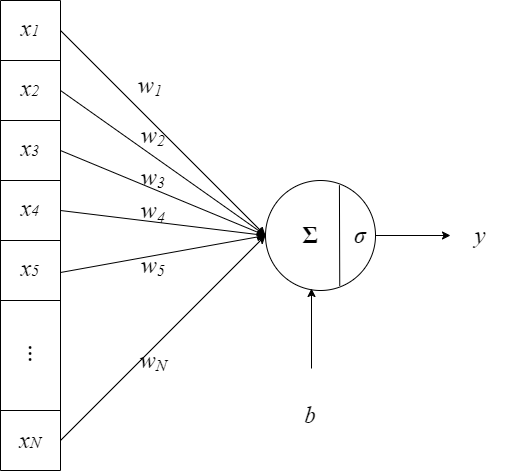
\includegraphics[width=0.5\linewidth]{figures/neuron.drawio.png}
    \caption{神經元示意圖}
    \label{fig:single-neuron}
\end{figure}


結合數個神經元的運算,羅氏(Rosenblatt)於 1958 年 \cite{rosenblatt_perceptron_1958} 提出感知器(Perceptron)模型。根據通用近似定理(Universal Approximation Theorem)\cite{funahashi_approximate_1989} ,感知器理論上可逼近任意函數。然而,後續研究發現單層的感知器具有如「線性不可分」\footnote{例如無法貼合異或(Exclusive OR,XOR)運算等函數} 等先天限制,使其曾經一度不被看好。

為了突破該缺陷,人們嘗試在輸入與輸出層之間增加「隱藏層(Hidden Layer)」,成為「多層感知器(Multilayer Perceptron,MLP)」,如圖 \ref{fig:mlp} 所示。藉助隱藏層的幫助,多層感知器可對輸入進行多次非線性轉換,大大拓展了模型的適用範圍。此模型是透過「加深隱藏層」得來,現今為人們熟知的「深層類神經網路(Deep Neural Network)」即由此得名。

\begin{figure}
    \centering
    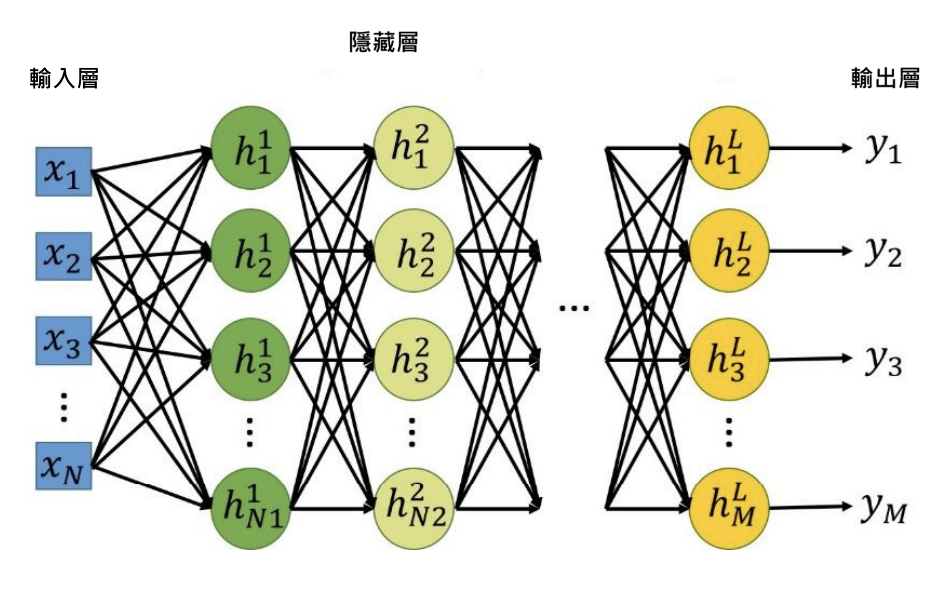
\includegraphics[width=0.8\linewidth]{figures/nnout.png}
    \caption{多層感知器/深層類神經網路示意圖}
    \label{fig:mlp}
\end{figure}


藉助深層類神經網路的彈性,我們可以透過⼤量訓練資料來訓練模型,藉此逼近應⽤任務中欲近似的函數 $f$,該函數蘊藏在資料集 $\mathcal{D} = \{(x_i, y_i)\}_{i=1}^N$ 中,其中每個資料點 $(x_i, y_i)$ 為輸入與輸出間的配對,即對於 $N$ 個資料點都有 $$y_i = f(x_i) \ \  \forall i \in \{1, \cdots\cdots, N\}$$之關係。
為了使這個函數更加逼近目標函數 $f$,
類神經網路會構建一個逼近中的函數 $f_{\theta_t}(\cdot)$ 。
透過不停的迭代,
模型對資料集 $\mathcal{D}$ 的每一筆資料 $x$ 給出預測 $f_{\theta_t}(x)$ 。
透過某個減損函數(Loss Function)$\mathcal{L}$ 計算出誤差(Error),
此誤差對參數 $\theta_t$ 求出梯度(Gradient)後將指示模型更新的方向,
以此乘上學習率(Learning Rate)$\eta$ 後從參數  $\theta_t$ 減去,便能對整個模型進行更新,使之更有機會接近目標函數 $f$。
由於此過程是依照梯度使得函數 $\mathcal{L}$ 逐步降低,以此獲名「梯度下降法(Gradient Descent)」,其公式如下:
$$\theta_{t+1} \leftarrow \theta_{t} - \eta \nabla_\theta\mathcal{L}(\mathcal{D}, f_{\theta_t}(\cdot))$$
其中,$t$ 為當前的迭代數,$\theta_t$ 為當前模型參數,$\theta_{t+1}$ 為更新後的模型參數。

在此模型更新的過程中,減損函數承擔著指引模型逼近的角色,因此根據應用的任務不同,常見的減損函數包括
\begin{itemize}
    \item 均方誤差(Mean Squared Error,MSE):一般用於迴歸(Regression)問題,直接計算兩數值之間的差距的平方和
    $$\mathcal{L}_{\text{MSE}}(y_i, \hat{y}_i) = \frac{1}{N} \sum_{i=1}^{N} (y_i - \hat{y}_i)^2$$

    \item 交叉熵(Cross-entropy,CE):一般用於分類(Classification)問題,著重計算兩個機率分佈之間的差異
    $$\mathcal{L}_{\text{CE}}(y_i, \hat{y}_i) = -  \sum_{i=1}^{N} \left[ y_i \log(\hat{y}_i) + (1 - y_i) \log(1 - \hat{y}_i) \right]$$
\end{itemize}

透過上述的訓練方式可以得知,類神經網路的訓練需要相當龐大且複雜的運算過程,因此剛提出時仍舊難以應用於現實應用中。

為了提高函數貼合的效率,魯氏(Rumelhart)與辛氏(Hinton)等人 \cite{rumelhart_learning_1986, rumelhart_learning_1987} 提出了反向傳播(Backpropagation)演算法,旨在將上述的更新過程,藉助鏈鎖率(Chain Rule)的幫助,由隱藏層逐層反向傳播至輸入層,對整個類神經網路進行修正。

反向傳播演算法的設計,正好能配合圖形處理器(Graphics Processing Unit,GPU)等硬體裝置的優勢,以平行運算能力加速函數貼合(Fit)的效率。由此開始,這種透過深層類神經網路,從大量資料集中發掘函數關係的機器學習演算法,被稱為深層學習(Deep Learning)。 類神經網路在各個領域的泛化能力(Generalizability)已經得到前所未有的效能,包含電腦視覺、語音處理和自然語言處理,因此深層學習在近年成為人工智慧發展的主流。

然而,根據資料特性的不同,並不是所有的資料都適用簡單的「輸入與輸出配對」的模式。研究者根據任務需求,發展出了不同架構的類神經網路以適應資料特性  。
前述最基本的深層類神經網路,由於資料是直接由輸入層,通過逐層的矩陣運算得到輸出,因此被稱之為「前饋式類神經網路(Feed Forward Network,FFN)」。

藉由調整各神經元之間的連接關係,發展出卷積式(Convolutional)、遞迴式(Recurrent)與轉換器(Transformer)類神經網路等架構變體,以適應如影像、語音和文字等不同型態的資料。這些架構在語音與文字處理被普遍使用,接下來將逐一分別介紹:

\subsection{卷積式類神經網路}
  
卷積式類神經網路(Convolutional Neural Network,CNN)為 1998 年由楊氏(Yann LeCun) \cite{lecun_gradient-based_1998} 提出,旨在以訊號處理的卷積(Convolution)運算,模擬生物的視覺皮質感知 \cite{hubel_receptive_1959} 。

\begin{figure}
    \centering
    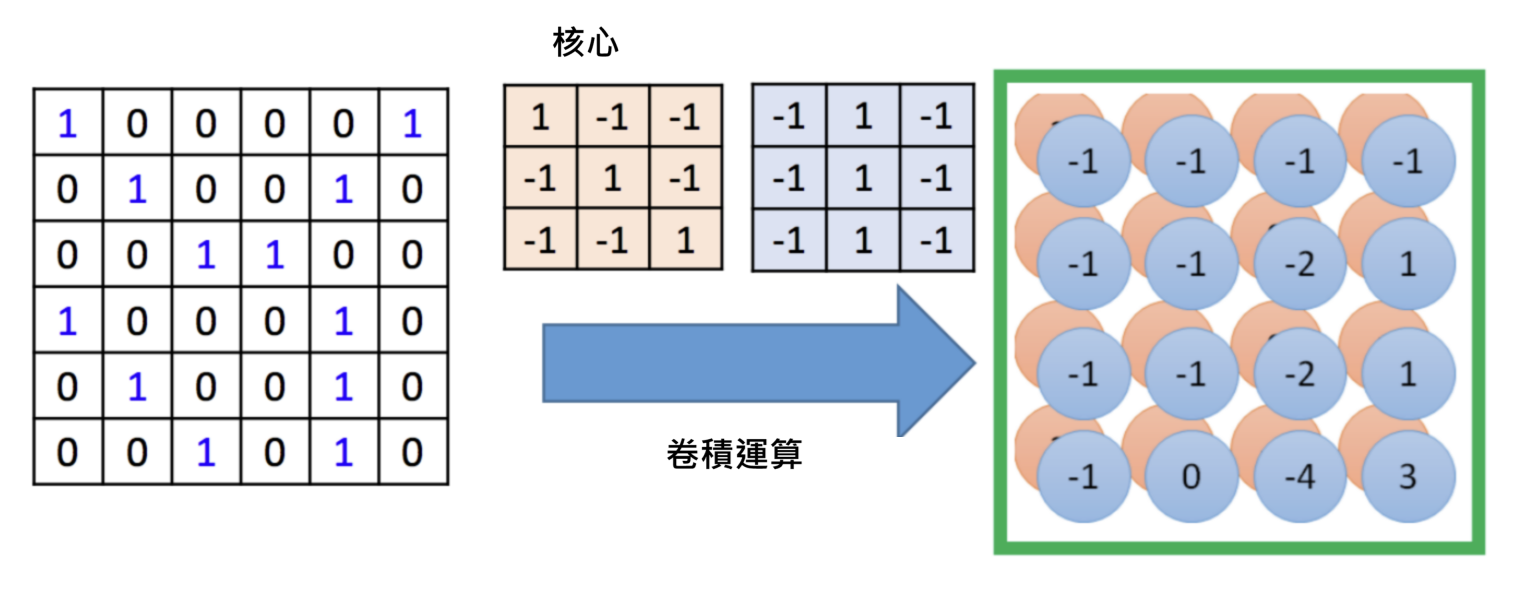
\includegraphics[width=0.9\linewidth]{figures/cnnnew.png}
    \caption{卷積式類神經網路示意圖,取自李宏毅教授的課程投影片}
    \label{fig:cnn}
\end{figure}

如圖 \ref{fig:cnn} 所示,卷積式類神經網路透過核心(Kernel),對輸入的資料 --- 如圖中的二維矩陣 --- 進行卷積運算,獲得該輸入的特徵圖(Feature Map)。核心帶來的移動不變性(Shift-invariance)非常適用於捕捉二維影像中的局部特徵,以作為類神經網路分辨資料的依據。

有別於影像處理中,資料多以二維矩陣表示像素 (Pixel)三原色的亮度數值,因此以二維的卷積運算為主;
由於語音時常處理時間軸之上的訊號,包含聲波波形(Waveform)、時頻譜(Spectrogram)或聲學特徵,因此一維的卷積式模型也時常出現,以模仿人耳聽覺對時變訊號的窗框(Window)的效應,進而觀察到語音中在不同解析度(Resolution)的資訊。


\subsection{遞迴式類神經網路與序列至序列模型}

\subsubsection{遞迴式類神經網路}
  
遞迴式類神經網路(Recurrent Neural Network,RNN)常用於處理隨時間變化的序列資料,特別是語音與文字等等,順序資訊相當關鍵的各種語言任務。

為了處理需要記憶和狀態的資料類型,
遞迴式類神經網路的輸出會重新接回輸入層,
使得前一個時間點(Timestep)的資料與內部狀態
會繼續影響後續的時間點。

常用的遞迴式類神經網路類型有長短期記憶(Long Short-term Memory,LSTM)\cite{hochreiter1997long} 和閘門循環單元(Gated Recurrent Unit,GRU)\cite{cho-etal-2014-properties} 等。

遞迴式類神經網路通常用在處理序列至序列的應用,例如語音辨識、語音合成或機器翻譯等和語言密切相關的任務中。

\subsubsection{序列至序列模型}
  
由於許多語言資料通常以兩個序列互相配對的形式呈現,因此專門處理這類資料的模型被稱為序列至序列模型(Sequence-to-sequence,Seq2seq)\cite{sutskever2014sequence}。此類模型的典型架構由編碼器(Encoder)和解碼器(Decoder)組成,旨在模擬輸入與輸出序列之間的變化與相依關係(Dependency)。

序列到序列模型一般有兩種模式:其一是每個時間點都生成一個輸出的向量,適用於輸入與輸出序列等長的任務,這種模式被稱為符記分類(Token Classification);但更常見的情況是,輸入與輸出序列的長度並不相同。處理後者的典型作法是讓編碼器將輸入序列依據時間,一步一步輸入編碼器,將序列編碼為內部表徵(Latent Representation)。完成編碼後,編碼器將最後一個時間點的表徵代表用以整個序列,稱為「語境向量(Context Vector)」。該向量接著被傳遞給解碼器,依序生成輸出序列。
\subsection{專注機制與轉換器類神經網路}

\subsubsection{專注機制}
  
由於遞迴式類神經網路需要處理整個序列的編碼和解碼資訊,對時間點距離較遠的輸入容易被遺忘,亦即難以處理長期相依性(Long-term Dependency)問題。為了解決這種困境,巴氏(Bahdanau)等人提出了「專注機制(Attention Mechanism)」\cite{bahdanau2014neural}。該機制讓解碼器將每個輸入序列的訊號都視作「部分的」語境向量,由對不同時間點的向量加權合計獲得,使得在生成輸出序列時能依據當時的需求從輸入序列中提取所需的訊息。專注機制的引入,使得序列至序列模型在處理如語音辨識、機器翻譯等任務時大大改善了效能。

\subsubsection{轉換器類神經網路}
  
儘管遞迴式類神經網路善於處理時序資料,但其難以平行化的架構限制了其在訓練和推理(Inference)時的效率。2017 年,瓦氏(Vaswani)等人 \cite{vaswani2017attention} 提出了完全由專注機制構成、不依賴遞迴運算的序列至序列模型,並稱之為「轉換器(Transformer)」,以解決機器翻譯等任務。

轉換器類神經網路一般包含編碼器和解碼器兩部分,均為多層架構。圖 \ref{fig:tfm_arch} 展示完整的轉換器架構圖,以下分別介紹其主要元件:

\paragraph{位置編碼(Positional Encoding)}

對於編碼器或解碼器的輸入序列,模型先對序列中不同位置的時間點進行編碼,取代遞迴式類神經網路逐步運算的過程,使其能在平行計算的同時考慮不同時間點的影響。編碼的函數可依照需求變換,如原始的轉換器採用三角函數進行位置編碼,而在語音模型中,有時也會採用卷積式網路以捕捉輸入的細微資訊。

經過位置編碼後,向量會通過每一個轉換器層(Transformer Layer),進行以多頭專注(Multi-head Attention)為主的一連串運算:

\paragraph{多頭專注}

轉換器層中的專注機制涉及三個輸入向量:詢向量(Query)$Q$、鑰向量(Key)$K$ 和值向量(Value)$V$。專注機制運算如下:
\[
\text{Attention}(Q, K, V) = \text{softmax}
\left(
\frac{QK^\top}{\sqrt{d_k}}
\right)
V
\]
其中 $\text{softmax}$ 為正規化指數函數,$d_k$ 為鑰向量 $K$ 的維度。這一運算首先通過鑰向量和詢向量的內積計算專注權重,而後為避免受維度過大影響而縮小為 $\sqrt{d_k}$ 分之一,最後通過正規化指數函數使得權重總和為 1 ,以此分配給值向量進行加權。

為應對多樣的輸入訊號,每個轉換器層具備多個獨立的專注機制,對三組輸入向量先進行各自不同的 $W^Q$、$W^K$、$W^V$ 線性轉換,稱為「多頭專注(Multi-head Attention)」。對於第 $i$ 個專注頭(Head)有
\[
\text{head}_i = \text{Attention}(QW^Q_i,KW^K_i,VW^V_i)
\]
最後,若有 $h$ 個專注頭,多頭專注模組會將多個頭的結果進行串接(Concatenate),經過線性轉換 $W^O$ 作為模組輸出
\[
\text{MultiHead}(Q, K, V) = \text{Concat}(\text{head}_1, \cdots\cdots, \text{head}_h) W^O
\]

\paragraph{其他層內運算}

每層轉換器層在經過多頭專注運算後,會依序進行以下三個步驟:

\begin{enumerate}
\item 與輸入向量透過殘差連接(Residual Connection)相加,隨後進行層正規化(Layer Normalization)以穩定訓練。
\item 將此結果通過一個簡單的前饋式類神經網路對向量做線性轉換。
\item 再將前饋網路的輸入與輸出再次計算殘差總和後,進行層正規化輸出。
\end{enumerate}

以上為轉換器被提出時的最原始模型,其後對殘差連接、層正規化的安排也存在各類變體。

\paragraph{跨專注機制(Cross-atttention)}

由於解碼器需要來自編碼器的輸入序列資訊幫助輸出,因此,原本在編碼器層中的自專注機制,在解碼器中會再經過一次跨專注機制的運算,使用編碼器提供的詢向量和鑰向量對解碼器的值向量進行專注運算。


\begin{figure}
    \centering
    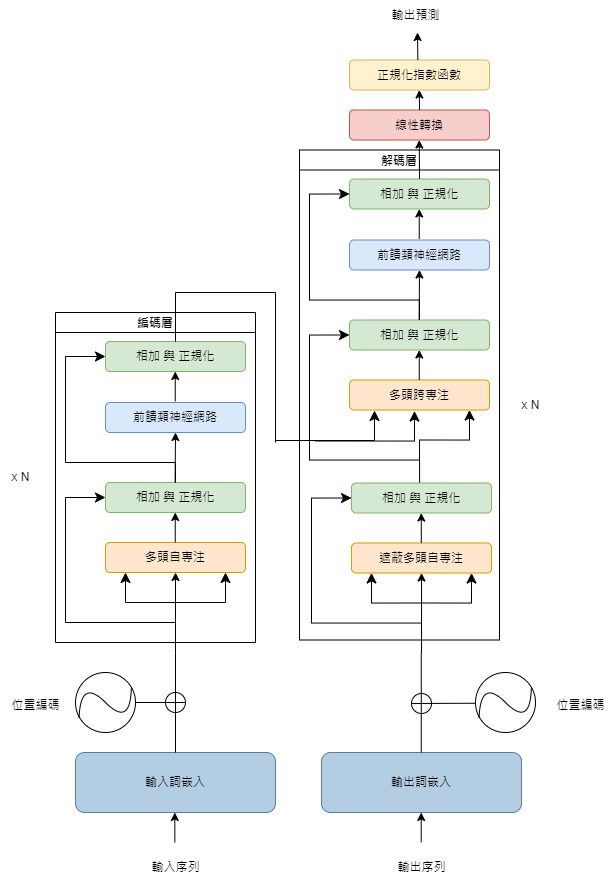
\includegraphics[width=0.9\linewidth]{figures/tfm_arch.drawio.png}
    \caption{轉換器架構圖}
    \label{fig:tfm_arch}
\end{figure}

由於轉換器不需要對每個時間點逐一運算,使其得以實現高度平行化,類神經網路得以透過專注機制同時進行序列資料的大量訓練。這種可擴展性(Scalability)使其在自然語言和語音處理上取得了巨大的進展,近乎取代了原先遞迴式類神經網路的應用場景,近年來甚至被應用在圖像類的資料上\cite{dosovitskiy2021image},展現了此種模型架構的彈性與泛用性,成為目前最前沿的人工智慧主流架構。

除了模型架構,機器學習中不可或缺的另一大部分是對資料的編碼過程。如何更有效率的讓機器理解、處理和輸出資料,是機器學習乃至深層學習的一大課題。面對捉摸不定、抽象且變化萬千的人類語言,語音和文字處理中的表徵學習尤為重要。
\section{表徵與自監督式學習}

\subsection{特徵抽取與表徵學習}
  
不論採用何種模型,為了讓機器可以處理並捕捉輸入資料中的訊號與模式(Pattern),如何對資料編碼和運算的步驟,在機器學習中稱之為特徵抽取(Feature Extraction)或表徵學習(Representation Learning),這是模型建構中不可或缺的重要步驟。

對於抽象的語言概念,早期工程領域根據對語音和文字的理解,分別進行了不同的處理。對於離散且可計數的文字,人們使用詞頻統計衍生出如 n 連詞(n-gram)、TF-IDF(Term-Frequency Inverse Document Frequency)等特徵作為模型學習的前處理步驟;而對於連續且複雜的語音,工程師則透過聲學原理與訊號處理的知識,使用如濾波器組(Filter Bank)、梅爾倒頻譜係數(Mel-Frequency Cepstrum Coefficient,MFCC)等特徵,類比人耳捕捉語音訊號的過程。

在深層學習逐漸發展的過程中,自然語言處理領域的一大里程碑是米氏(Mikolov)提出的「word2vec」模型 \cite{mikolov_efficient_2013},該模型以連續的向量表徵(Vector Representation)取代稀疏(Sparse)的統計數據,對離散的文字單詞進行「詞嵌入(Word Embedding)」編碼。通過大量文本運算,將各單詞之間的共現(Collocation)以跳躍詞(Skip-gram)、連續詞袋(Continuous Bag-of-Word,CBOW)等演算法轉換成高維向量空間中的點,找出每個單詞最適合的語義表徵。爾後,為了更細緻地捕捉同一單詞在不同句子中的脈絡變化,ELMo(Embeddings from Language Model)\cite{peters_deep_2018} 提出了「脈絡化詞嵌入(Contextualized Embedding)」的概念,使得各單詞在運算表徵的過程中可以根據上下文進行些微調整。

\subsection{自監督學習}
  
隨著轉換器模型的提出,BERT(來自轉換器的雙向編碼器表徵,Bidirectional Encoder Representations from Transformers)\cite{devlin_bert_2019} 被提出。通過自專注機制,工程師們無需依賴人工標記,透過預先設定任務(Pretext Task)引導模型從大量文本中自行找出更細緻且考量脈絡(Contextualized)的語義關係,並在許多文字任務上獲得了優異的成績。

自此,楊氏(Yann LeCun)將這種以特定任務作為引導、藉助資料本身的結構替代標註,從大量未標註資料中進行學習資料模式(Pattern)的訓練方式,稱之為「自監督學習(Self-supervised Learning,SSL)」。BERT 的成功使自監督學習得以大行其道,並出現了許多由巨量資料進行預訓練(Pre-train)的基石模型(Foundation Model),有效解決了語言處理領域中的標註資料稀缺的問題。人們在解決語言相關任務時,不需從頭蒐集資料與進行耗時耗能的訓練過程,而是可以利用基石模型優良的泛化(Generalization)能力,解決各種應用任務的需求。相比於預訓練的任務,這些更貼近日常現實的任務被稱為「下游任務(Downstream Task)」,能應對廣泛的下游任務種類,這是基石模型最大的優勢。

有鑑於文字處理方面的成功,語音領域的研究者嘗試將相似模式應用於語音,眾多語音基石模型隨之出現。這些大量的語音資料庫幫助模型萃取出有助於下游任務的語音表徵(Speech Representation),在各種任務上獲得了優於傳統聲學特徵的表現。語音表徵具備的無窮潛力,逐漸成為聲學特徵之外的新選擇。

依照這些語音自監督模型的預訓練學習模式,可大致分為重建式、預測式與對比式模型。以下分別介紹這三類模式:

\subsubsection{重建式學習(Reconstruction Learning)}

此類模型通過對輸入訊號進行擾動(Perturb)後,期望模型將被更動的輸入重新預測回原始資料,通常減損函數表示為:
$$\mathcal{L}_{recon} = \mathbb{E}_x[|f_\theta(\tilde{x}) - x|]$$
其中 $\tilde{x}$ 為擾動後的資料,$f_\theta(\cdot)$ 為模型函數。擾動方式通常以遮蔽為主,在文字處理中以 BERT 為代表,稱為「遮蔽語言模型(Masked Language Model,MLM)」。在語音中,採用此方式學習的有 Mockingjay \cite{liu_mockingjay_2019}、TERA \cite{t_tera_2021} 等模型。  % NPC

\subsubsection{預測式學習(Predictive Learning)}

此類模型通過預訂一些學習目標函數,製造類似輸入與輸出的配對資料,讓模型預測該函數的結果來學習資料中的特定結構。其訓練減損函數可表示為:
$$\mathcal{L}_{pred} = \mathbb{E}_x[\text{eval}(f_\theta(x), \hat{f}(x))]$$
其中 $\hat{f}$ 是期望模型學習的目標函數,$f_\theta(\cdot)$ 為模型函數,$\text{eval}$ 是用來評估預測好壞的標準。

目標函數的典型代表是自迴歸(Autoregressive),期望模型預測未來時間點的輸入表徵。文字方面以生成式預訓練轉換器(Generative Pretrained Transformer,GPT)系列 \cite{radford_language_nodate, brown_language_2020}為代表,語音上的自迴歸預測編碼(Autoregressive Predictive Coding,APC) \cite{chung_generative_2020} 也是採用此種模式。此外,語音基石模型還可以使用其他訓練目標,如 PASE+ \cite{ravanelli_multi-task_2020} 預測其他模型的表徵,而本文著重探究的「隱藏單元 BERT(Hidden-unit BERT,HuBERT)」\cite{hsu_hubert_2021, hsu_hubert_2021-2} 則以預測分群(Cluster)後的輸入表徵為目標,這些預測目標又被視為偽標註(Pseudo-label),後文將著重探討。

\subsubsection{對比式學習(Contrastive Learning)}

此學習方式的訓練目標是要求模型區分正樣本(Positive Sample)與負樣本(Negative Sample)的差異,減損函數通常定義為:
$$\mathcal{L}_{contr} = -\mathbb{E}_x\left[\log
\left(
{\frac
{\sum_{\tilde{x} \in x_{pos}}\exp(\text{sim}(x, \tilde{x}))}
{\sum_{\tilde{x} \in \mathcal{X}}\exp(\text{sim}(x, \tilde{x}))}
}\right)\right]$$

其中 $x$ 為輸入,$x_{pos}$ 為正樣本,$\mathcal{X}$ 為包含正負樣本的資料集,$\text{sim}(\cdot, \cdot)$ 是評估兩個樣本相似程度的函數,常用的相似度函數為內積運算得出的餘弦相似度(Cosine Similarity)。語音上最早使用對比式學習的模型為對比預測編碼(Contrastive Predictive Coding,CPC)\cite{maekaku2022speech},之後如 Wav2vec \cite{schneider2019wav2vec}、Modified CPC \cite{rivière2020unsupervised}、Wav2vec 2.0 \cite{baevski2020wav2vec} 等模型亦是以對比正負樣本的模式訓練,但訓練時正負樣本的定義有所差異,如 Wav2vec 僅以時間維度上相同的向量為正樣本,其餘則將固定時間內的向量皆視為正樣本。

對比式學習通過正負樣本的定義,將預訓練任務形塑為分類問題,因此減損函數本質上為交叉熵,使模型能夠判斷訓練資料中的結構差異。

\subsection{向量量化與離散單元}
  
語音訊號雖然記錄語言資訊,卻與影像資料一樣都是連續數值資料,不像離散的文字較易處理,因此發展出了許多應用廣泛的模型。為了使語音模型訓練可以套用自然語言處理領域的演算法,從連續語音中找出離散表徵逐漸成為研究趨勢,這類研究被稱為「聲學單元發掘(Acoustic Unit Discovery,AUD)」。

由於語言概念本質上是離散符號,向量量化技術常用於涉及語言標註的情境,如電腦視覺經典的量化向量變分自編碼器(Vector-Quantized Variational Autoencoder,VQ-VAE)\cite{van2017neural},利用影像標註的離散語言單詞特性,使模型學習的表徵向量被約束在編碼簿(Codebook) 的幾個向量中。

% 將模型的連續特徵透過甘式軟性最大化和 K-平均兩種向量量化技術
在語音領域,基於 Wav2vec 之上的 Vq-wav2vec \cite{baevski2019vq} 和 Wav2vec 2.0 將連續的語音特徵量化加入訓練目標中,在語音辨識等任務上取得了顯著進步。

HuBERT \cite{hsu_hubert_2021-2} 則應用先對連續的 MFCC 特徵進行 K-平均(K-Means)演算法分群,以所得的群心(Centroid)編號作為訓練目標,實施類似 BERT 的遮蔽語言模型訓練,
並改以此次訓練得到的語音表徵為目標,再次分群後實施第二次訓練。 
這些經過兩輪訓練後,從模型表徵分群得到的群心,被視為「隱藏單元(Hidden Unit)」,編碼了語音訊號中的代表性聲學特徵。透過找出隱藏單元的過程,HuBERT 在低資源情況下達到與 Wav2vec 2.0 相近的語音辨識成績。

\subsection{無文字(Textless)架構}
  
奠基於 HuBERT 等語音基石模型的成功,利用隱藏單元的概念,將大量語音資料表徵進行 K-平均演算法,作為這些語音訊號的偽標籤。如此得到的大量離散隱藏單元形成了「偽文字(Pseudo-text)」的語料庫,基於這些離散單元訓練語言模型,稱為「生成式口語語言模型(Generative Spoken Language Model,GSLM)」\cite{lakhotia_generative_2021-1}。配合反向語音合成訓練基於離散單元的語音生成模型,整體架構不依賴文字標註,訓練出純語音語言模型,稱為「無文字(Textless)架構」\cite{noauthor_textless_2021}。

無文字模式在語音問答(Spoken Question Answering)\cite{lin2022dual}和語音到語音翻譯 (Speech-to-speech Translation)\cite{chen_speech--speech_2023}中取得了前所未有的進展。這些「離散單元(Discrete Unit)」被視為類似文字卻不依賴人類文字標記的語音表徵,具有儲存位元率低和可套用文字語言模型訓練模式的優勢,受到語音社群的廣泛借鑑,後續也帶出了許多如\cite{zhang2024speechtokenizer} 等將語音以離散表徵編碼的研究。

雖然在系統與應用任務上取得了成功,但這些離散單元本身與文字的差異,及其對語音語言模型訓練的幫助,仍是領域內探討的焦點。有鑑於此,本論文基於語言知識,從最接近文字且與語音訊號最相關的「音位(Phoneme)」開始探討,期望了解離散單元能帶來的特徵及其對後續應用的幫助。

\section{本章節總結}
  
本章節首先介紹了深層學習模型的核心部件 --- 類神經網路的基本原理,隨後對本論文研究的核心 --- 「語音表徵」與「離散單元」的發展與歷史進行了梳理。接下來的章節將緊扣這些基石模型得到的離散特徵,對其與「音位」這類語音學標記之間的統計關係進行更深入分析。

% %% textless --> 是不是要補一下模型敘述?
% 補 citations
% 順搞,包含表格邊框
% 算 ratio 有必要嗎?
% $$ 長條圖分開討論?
% alignment
% 換 dev

%%% https://arxiv.org/pdf/2102.01192

% mycites
% 最後!處理數據作圖…!! 是要多久……啊就那樣
% phone type

\chapter{單一語音離散表徵與音位的關係}  % 與語音標記的對應模式

  HuBERT \cite{hsu_hubert_2021, hsu_hubert_2021-2} 和 Wav2vec 2.0 \cite{baevski2020wav2vec} 等語音基石模型的成功,
不僅在語音任務上達到了前所未有的表現,
還促進了語音表徵離散化的發展。
由此產生的「無文字(Textless)」架構 \cite{noauthor_textless_2021, lakhotia_generative_2021, lakhotia_generative_2021-1},讓人們在處理語音訊號時,有了連續表徵以外的新選擇。
離散形式的表徵可以直接應用文字領域發展的技術,
如機器翻譯、生成式模型等,為語音技術帶來新的突破。另一方面,基於離散「符記(Token)」的共同形式,
離散語音表徵可以更好的整合文字資料,
促成多模態領域的發展。跨模態離散表徵的成功,
甚至驅使影像領域也開始發展離散表徵,  % 要確認一下「開始」嗎?
如探討唇語的 AV-HuBERT \cite{shi2021learning} 等等,展現了離散表徵在資料處理上的優勢。
  % 不是模型運算
% 還有影像的 vokenization \cite{tan-bansal-2020-vokenization} 等等。好像更早
% TODO: 找到影像那邊的新的 token?

% 語言學那邊只有一般語音?還是包含 acoustic phon 嗎?
此外,除了技術的角度切入,為了探討離散語音表徵成功背後的可能因素,
以及它們與語言學對人類語音理解之間的差異,
甚至是進一步利用這些技術協助更細緻的探討人類的語音現象。
因此,原先在連續語音表徵上的語音學分析,
也開始關注離散表徵在多大程度上能描述語音現象,
將其列入考量,成為除了連續語音特徵和時頻譜之外的另一個選擇。
% TODO: cite  "is cont necessary? 那篇"
% 更由於這些離散表徵形式上和音位、文字的相似性,  %% 這個好像還沒?
%% 他們還是更喜歡 IPA,只是先當成一種新的 label 吧?

\section{相關研究}

\subsection{無文字與離散語音表徵}

  自 HuBERT 帶起的研究之後,
出現了愈來愈多離散表徵相關的研究,
例如 \cite{10097097, abdullah23_interspeech, chang_exploration_2023, liu2024dinosr, zhang2024speechtokenizer, huang2023repcodec} 等等。
它們在提出自己的離散表徵時,
也會採取 HuBERT 的
衡量方式,
% 例如 PNMI 等等的,
來驗證這些離散單元與語音中的內容及人類對語音的詮釋之間
具有一定程度的相關性,
並從資訊理論(Information Theory)的角度,
證明這些離散單元
確實具備區分
不同語音
% 中不同形式的
資訊
的能力
。

\subsection{語音學分析}

  
由於語音處理本身最終是針對人類語音,
因此
有一群研究者通過對人類語音的理解,
將這些知識應用在分析模型如何對語音訊號建構表徵之上。例
如 \cite{deseyssel22_interspeech, wells_phonetic_2022, 10097097, abdullah23_interspeech} 等研究。
% 就韋誠說的妹子那篇嗎?

        基於這些作品
對語音離散表徵的興趣和探討,  % 其實是我的興趣?
本論文也先透過過往幾個常用來分析語音表徵的方式,特別是
HuBERT \cite{hsu_hubert_2021-2} 提出的標準進行初步的分析。
        % 以下介紹此次分析語音表徵的衡量方式:

\section{衡量方式}

  
% 首先是
本次研究主要探討純度(Purity)、熵(Entropy)和相互資訊(Mutual Information,MI)等指標,
這些標準在 HuBERT 中採用 \cite{hsu_hubert_2021, hsu_hubert_2021-2},用於比對機器學習過程中得到的偽標註與人類標註之間的相關性(Correlation)。以下對各標準進行詳細解釋:

        不論是何種語音基石模型,
語音表徵的基本單位是音框(Frame)。因此一段語句(Utterance)的語音離散單元被表示為 $[y_1, \cdots\cdots, y_T]$。其中 $T$ 是該段語句的音框總數。對於該段語句,若給予一段在音框上對齊的語音學標註(Phonetic Label) $[z_1, \cdots\cdots, z_T]$,此時我們可以將離散單元與標註之間配對的出現次數,寫為一個雙變數的共同分佈(Joint Distribution)
    \begin{align}
      p_{yz} = \frac{\sum^T_{t=1}[{y_t = i \wedge z_t = j}]}{T}
    \end{align}

其中 $i$ 是第 $i$ 個音位類別,而 $j$ 指編號為$j$的離散單元。兩個變數的邊際機率(Marginal Probability)分別為
    \begin{align}
    p_z(j) &=\sum_i{p_{yz}(i, j)} \\
    p_y(i) &=\sum_j{p_{yz}(i, j)} 
\end{align}

因此,對於每一個音位 $i$ 而言,這個音位對應最可能的離散單元為
    \begin{align}
      z^\ast(i) = \arg\max_j p_{yz}(i, j)
    \end{align}
與之相對應的,對於每一個離散單元的類別 $j$ 則可以找到機率最高的音位
    \begin{align}
      y^\ast(j) = \arg\max_i p_{yz}(i,j)
    \end{align}

% 於是我們可以計算出以下指標:
透過這些定義,以下分節介紹將要分析的指標:

\subsection{純度}

        本指標考慮音位和離散單元兩個序列之間對應的最高機率,因此從音位與離散單元的角度出發,可以得到以下兩項數據:

\paragraph{音位純度(Phoneme Purity)}

        考慮每個離散單元對應的音位中,最高機率音位的機率,表示為
    \begin{align}
      \mathbb{E}_{p_z(j)}\left[p_{y|z}(y^*(j)|j) \right]
    \end{align}

此指標表示該單元是否對其對應的音位有足夠的代表性。

\paragraph{分群純度(Cluster Purity)}

        與音位純度相對,改以每個音位的角度,考慮對應單元類別的機率
    \begin{align}
      \mathbb{E}_{p_y(i)}\left[p_{z|y}(z^*(i)|i) \right]
    \end{align}

        由於離散表徵進行分群演算法時的類別數是一項超參數(Hyperparameter),且通常離散單元的分群數量會比音位多,因此該統計數據本身不直接具有語音學的解釋意義,而且在分群數量很多時會顯著下降。
然而該指標在考量音位純度時必須一併考慮,
因為當分群數非常多時,分群純度過低
暗示離散單元做不到歸納音位類別的效果,
使得音位純度失去其意義。一個極端的情形是每一個音框都給予不同的離散單元編號,如此音位純度可以達到
         100\%。

\subsection{熵和相互資訊}

  除了純度提供「最高機率」的對應關係,根據 HuBERT 論文 \cite{hsu_hubert_2021-2} 中的分析方式,我們也可以從資訊理論的角度,觀察兩個序列的熵和相互資訊。

\paragraph{熵(Entropy)}

  熵的定義按照資訊理論,衡量兩個序列中標籤類別出現機率的不確定性(Uncertainty),公式寫作:
    \begin{align}
        H(y) &= \sum_i{p_y(i)\log p_y(i)} \\
        H(z) &= \sum_j{p_z(j)\log p_z(j)}
    \end{align}
其中 $H(y)$ 和 $H(z)$ 分別為音位和離散單元的熵,數值愈高分別表示各種音位和離散單元出現的機率愈平均。

\paragraph{以音位標準化之相互資訊(Phone-normalized Mutual Information,PNMI)}

  本數據以「觀察到某一個離散單元,能降低多少音位標註的不確定性」,定義該離散單元的出現背後提供了多少音位的資訊。公式寫為:
    \begin{align}
        \frac{I(y;z)}{H(y)}&=\cfrac{\sum_i \sum_j p_{yz}(i, j) \log \cfrac{p_{yz}(i, j)}{p_y(i)p_z(j)}}{\sum_i p_y(i) \log p_y(i)} \\
        &=\frac{H(y)-H(y|z)}{H(y)} \\
        &=1-\frac{H(y|z)}{H(y)}
    \end{align}

        該項數據愈高,表示離散單元的分群愈能提供語音音位的資訊,是一個品質更好的分群結果。由於離散單元能多好的對應到音位才是人們所關心的問題,因此與純度不同,只以音位的角度出發,而不考慮以離散單元分群的角度。

% \input{3b}

\section{語音學分類(Phone Type)}

% \subsection{簡介}

  除了單一音位本身的特性以外,由於音位之間存在相似的特徵,可以分成幾個組別。
依照 \cite{10097097, abdullah23_interspeech} 的分組方式,對英語的音位進行分類並合併比對數據,
觀察這些離散單元是否有擷取到相似的發聲特徵,而不單純只是把音位分成約 50 類完全獨立的標籤。以下簡介六個音位組別:

% (基於語音表徵本身就是 acoustic sisgnals 來的,應該 by nature 要可以對語音特徵分組吧?)

        % 英語中的音位依照發音的方式,共分成七個類別。

\begin{itemize}
    \item 塞音(Plosive):以完全阻塞氣流的方式發音的音位,包含 /p/、/b/、/t/、/d/、/k/、/g/ 六種
    \item 擦音(Fricative):藉由在口腔中形成的縫隙,使氣流通過時摩擦形成的發音,包含 /f/、/v/、/s/、/z/、/\textesh/ (sh)、/\textyogh/ (如「garage」的 「-ge」)、/θ/ (無聲的 th)、/ð/ (有聲的 th)、/h/ 九種
    \item 塞擦音(Affricate):由塞音和同部位的擦音同時發出的輔音,英語中只有 /t\textesh/ 和 /d\textyogh/ 兩種,即 ch 和 j 的發音
    \item 鼻音(Nasal):使氣流通過鼻腔形成的聲音,有 /m/、/n/、/ŋ/ (ng) 三種
    \item 近音(Approximant):又稱半元音,為介於元音和輔音之間的聲音,有 /j/ (為 y 作為輔音時的發音)、/r/、/l/、/w/
    \item 元音(Vowel):可自成音節的音位,包含發音位置固定的單元音(Monophthong)和會移動的的雙元音(Diphthong),通常以 a、e、i、o、u 字母產生的聲音皆屬於此類別
\end{itemize}


% \paragraph{元音}

% 母音在這邊為了簡單起見,會被分在一起?

% 根據發音的位置是否發生改變,英語的元音可分為:

% \begin{itemize}

% 兩大類別。

% \paragraph{輔音}

% 而輔音按照發音的方式,可分為以下五類:

% \subsection{解釋意義}

% \begin{itemize}
    % \item 純度(Purity):換成以語音學的類別作為新的語音標籤後,有何變化(關聯性更強?)
    % \item 熵(Entropy)(放直方圖解釋) \(\rightarrow\) 語音分類更明顯?
    % \item 對齊(Alignment):是否減少分段資訊的保留(連續子音母音被合併?)
% \end{itemize}

透過將音位分組後,形成新的語音標註,並重新分析統計指標,觀察在純度等數據是否顯示離散單元與語音的發音方式具有更明確的關聯性。


\section{實驗集與分析模型}

%%%%%%%%%
%%%%%%%%%% %%%%%%%%%%%%%%%%
%%%%%%%%%% 本研究的分析對象參考無文字架構 \cite{noauthor_textless_2021, lakhotia_generative_2021, lakhotia_generative_2021-1} 的研究,採用當中提及的 CPC、Wav2vec 2.0 和 HuBERT 三個語音基石模型,並與作為比對的聲學特徵梅爾時頻譜(Mel-Spectrogram),共四種語音表徵模型。模型的詳細資訊如表 \ref{tab:model-info} 所示:
%%%%%%%%%
%%%%%%%%%% \begin{table}
%%%%%%%%%%     \centering
%%%%%%%%%%     \begin{tabular}{|c|l|c|c|} \hline 
%%%%%%%%%%          語音表徵&   模型架構&離散表徵來源層數& 時間解析度(Time Resolution)\\ \hline 
%%%%%%%%%%          HuBERT      &   CNN + Transformer&6& 20 毫秒\\ \hline 
%%%%%%%%%%          Wav2vec 2.0 &   CNN + Transformer&14& 20 毫秒\\ \hline 
%%%%%%%%%%          CPC         &   CNN + GRU&2& 10 毫秒\\ \hline 
%%%%%%%%%%          LogMel      &   聲學特徵&N/A& 10 毫秒\\ \hline
%%%%%%%%%%     \end{tabular}
%%%%%%%%%%     \caption{語音離散表徵的來源層數與音框時間解析度}
%%%%%%%%%%     \label{tab:model-info}
%%%%%%%%%% \end{table}
%%%%%%%%%
%%%%%%%%%% 以下是各語音表徵模型的簡介:
%%%%%%%%%
%%%%%%%%%% \begin{itemize}
%%%%%%%%%%     \item **CPC(對比預測編碼)**:CPC 由編碼器和預測器兩部分組成。編碼器從語音輸入生成嵌入 z。預測器基於過去預測編碼器的未來狀態,系統通過對比損失進行訓練。我們使用 Rivière 和 Dupoux(2020)訓練的 CPC 模型,該模型使用 LibriLight 數據集的6k小時“乾淨”子樣本進行訓練。我們從預測器的中間層提取表示,生成256維的嵌入(每10毫秒一個),如原始論文所述。
%%%%%%%%%%     \item **Wav2vec 2.0**:此模型使用編碼器和預測器,並通過對比性地區分編碼器輸出中的正樣本和負樣本進行訓練。我們使用 Baevski 等人(2020b)訓練的預訓練 Wav2vec 2.0 LARGE 變體,該模型在 LibriLight 數據集的60k小時上進行訓練。此模型將原始音頻編碼為1024維的向量幀(每20毫秒一個)。為了選擇最佳層,我們從模型的每一層提取10小時的 LibriLight 子集的凍結表示,並使用 CTC 損失訓練線性分類器來預測文本標籤的音素版本。第14層在 LS dev-other 上獲得了最低的 PER(Baevski 等人,2021年使用類似的方法選擇了第15層)。
%%%%%%%%%%     \item **HuBERT**:與 CPC 和 Wav2vec 2.0 使用對比損失不同,HuBERT 使用類似於 BERT(Devlin 等人,2019)的掩碼預測任務進行訓練,但輸入是掩碼連續音頻信號。目標是通過對原始語音特徵或早期迭代的學習特徵進行無監督聚類獲得的,這一方法受 DeepCluster(Caron 等人,2018)的啟發。我們使用了 Hsu 等人(2021)訓練的 BASE 12 層變壓器模型,該模型在960小時的 LibriSpeech 上進行了兩次迭代訓練。此模型在每層將原始音頻編碼為768維的向量幀(每20毫秒一個),我們從第6層提取這些向量,如原始論文所述。
%%%%%%%%%%     \item **LogMel**:作為基準,我們考慮使用80個頻帶的對數梅爾濾波銀行編碼器。
%%%%%%%%%% \end{itemize}
%%%%%%%%%% %================


%%%%%%%%%%%%%%%%
  本研究的分析對象參考無文字架構 \cite{noauthor_textless_2021, lakhotia_generative_2021, lakhotia_generative_2021-1} 的研究,
% 採用當中提及的 CPC、Wav2vec 2.0 和 HuBERT 三個語音基石模型,並與作為比對的聲學特徵梅爾時頻譜(Mel-Spectrogram),共四種語音表徵模型。
% 模型的
% 資訊簡述如下:
採用論文中提及的四種語音表徵,簡述如下:

\begin{itemize}
    \item CPC:卷積式編碼器 + 遞迴式預測器,以對比式學習訓練。表徵來自預測器的中間層,每 10 毫秒提取一個向量表徵作為音框
    \item Wav2vec 2.0:卷積式編碼器 + 轉換器預測器,以對比式學習訓練。表徵來自轉換器第 14 層,每 20 毫秒作為一個音框
    \item HuBERT:卷積式編碼器 + 轉換器預測器,以預測式學習訓練,其訓練目標為 K-平均分群演算法的結果,透過遮蔽語言模型的方式訓練。表徵來自轉換器第 6 層,每 20 毫秒作為一個音框
    \item LogMel:為 80 維對數梅爾時頻譜的聲學特徵,在此作為比較基線(Baseline)。音框寬度為 10 毫秒
    
    % CPC 由編碼器和預測器兩部分組成。編碼器從語音輸入生成嵌入 z。預測器基於過去預測編碼器的未來狀態,系統通過對比損失進行訓練。我們使用 Rivière 和 Dupoux(2020)訓練的 CPC 模型,該模型使用 LibriLight 數據集的6k小時“乾淨”子樣本進行訓練。我們從預測器的中間層提取表示,生成256維的嵌入(每10毫秒一個),如原始論文所述。
    % \item Wav2vec 2.0:此模型使用編碼器和預測器,並通過對比性地區分編碼器輸出中的正樣本和負樣本進行訓練。我們使用 Baevski 等人(2020b)訓練的預訓練 Wav2vec 2.0 LARGE 變體,該模型在 LibriLight 數據集的60k小時上進行訓練。此模型將原始音頻編碼為1024維的向量幀(每20毫秒一個)。為了選擇最佳層,我們從模型的每一層提取10小時的 LibriLight 子集的凍結表示,並使用 CTC 損失訓練線性分類器來預測文本標籤的音素版本。第14層在 LS dev-other 上獲得了最低的 PER(Baevski 等人,2021年使用類似的方法選擇了第15層)。
    % \item HuBERT:與 CPC 和 Wav2vec 2.0 使用對比損失不同,HuBERT 使用類似於 BERT(Devlin 等人,2019)的掩碼預測任務進行訓練,但輸入是掩碼連續音頻信號。目標是通過對原始語音特徵或早期迭代的學習特徵進行無監督聚類獲得的,這一方法受 DeepCluster(Caron 等人,2018)的啟發。我們使用了 Hsu 等人(2021)訓練的 BASE 12 層變壓器模型,該模型在960小時的 LibriSpeech 上進行了兩次迭代訓練。此模型在每層將原始音頻編碼為768維的向量幀(每20毫秒一個),我們從第6層提取這些向量,如原始論文所述。
    % \item LogMel:作為基準,我們考慮使用80個頻帶的對數梅爾濾波銀行編碼器。
\end{itemize}


% \ref{tab:model-info} 所示:

% \begin{table}
%     \centering
%     \begin{tabular}{|c|l|c|c|} \hline 
%          語音表徵&   模型架構&離散表徵來源層數& 時間解析度(Time Resolution)\\ \hline 
%          HuBERT      &   CNN + Transformer&6& 20 毫秒\\ \hline 
%          Wav2vec 2.0 &   CNN + Transformer&14& 20 毫秒\\ \hline 
%          CPC         &   CNN + GRU&2& 10 毫秒\\ \hline 
%          LogMel      &   聲學特徵&N/A& 10 毫秒\\ \hline
%     \end{tabular}
%     \caption{語音離散表徵的來源層數與音框時間解析度}
%     \label{tab:model-info}
% \end{table}
我們使用該論文釋出之預訓練模型與 K-平均量化模型。預訓練模型細節詳述於 \cite{lakhotia_generative_2021-1} 中,量化模型則是該篇論文透過公開的 LibriSpeech 資料集 \cite{panayotov_librispeech_2015} 中 train-clean-100 訓練集
,獲取語音表徵後執行 K-平均分群演算法所得,並釋出群數為 50、100 和 200 的三個版本。

% 此後亦跟隨該研究選用特定模型層數及其釋出之 K-平均量化模型。這些模型層數與量化模型在該研究中被證明與語音學特徵最相關,且被使用於無文字架構後續研究之語音離散表徵的抽取方法。無文字研究中 \cite{lakhotia_generative_2021-1} 已透過公開的 LibriSpeech 資料集之 train-clean-100 訓練集
% 語料
% 對四種語音表徵進行 K-平均分群演算法,分別得到群數為 50、100 和 200 的三個量化模型。

        % 本論文以公開的 LibriSpeech 資料集為分析對象,採取其 train-clean-100 為分析的語音語料庫。
        本論文亦以 LibriSpeech train-clean-100 作為分析對象,
% 因此,
% 本研究
將語音語料庫的語音資料經過四個模型獲取連續表徵後,再經過量化模型得到完全由離散單元組成的「偽文字」語料。

        針對語音學的音位標註,透過強迫對齊器(Forced-aligner)\footnote{https://github.com/MontrealCorpusTools/Montreal­Forced­Aligner}的英語預訓練模型,從語料庫的文字轉寫取得語音資料的音位標註與對應的時間範圍。最後透過語音表徵各自的時間解析度生成以音框為單位的音位標註語料。最後將兩者對語音資料集進行音位標註相關性的分析。
%================

\section{分析結果}

%% (((還是放一下長條圖說個事兒好了)))     

\subsection{基於各自音位的分析}

        \begin{table}[!htbp]
            \centering
            \begin{subtable}[t]{\textwidth}
                \centering
                \begin{tabular}{|c|c|c|c|c|c|} \hline 
                                & 音位純度 & 分群純度 & 音位熵 & 離散單元熵 &    PNMI \\ \hline 
                    HuBERT      &   0.5256 &   0.3382 & 3.3152 &     3.8681 & 0.4993 \\ \hline    %% 1.6552 h
                    Wav2vec 2.0 &   0.4006 &   0.2676 & 3.3152 &     3.8215 & 0.3706 \\ \hline    %% 1.2286 w
                    CPC         &   0.5188 &   0.3812 & 3.3146 &     3.7918 & 0.4992 \\ \hline    %% 1.6545 c
                    LogMel      &   0.3253 &   0.1473 & 3.3158 &     3.8630 & 0.2647 \\ \hline    %% 0.8776 l 
                \end{tabular}
                \caption{群數 = 50}
                \label{tab:ch3-clu050-phn}
            \end{subtable}        

            \vspace{0.5cm}        

            \begin{subtable}[t]{\textwidth}
                \centering
                \begin{tabular}{|c|c|c|c|c|c|} \hline 
                                & 音位純度 & 分群純度 & 音位熵 & 離散單元熵 &    PNMI \\ \hline 
                    HuBERT      &   0.6097 &   0.2553 & 3.3152 &     4.5704 & 0.5786 \\ \hline    %% 1.9181 h
                    Wav2vec 2.0 &   0.4877 &   0.2118 & 3.3152 &     4.5284 & 0.4596 \\ \hline    %% 1.5235 w
                    CPC         &   0.5895 &   0.2674 & 3.3146 &     4.5034 & 0.5557 \\ \hline    %% 1.8418 c
                    LogMel      &   0.3348 &   0.0931 & 3.3158 &     4.5591 & 0.2789 \\ \hline    %% 0.9247 l 
                \end{tabular}
                \caption{群數 = 100}
                \label{tab:ch3-clu100-phn}
            \end{subtable}        

            \vspace{0.5cm}        

            \begin{subtable}[t]{\textwidth}
                \centering
                \begin{tabular}{|c|c|c|c|c|c|} \hline 
                                & 音位純度 & 分群純度 & 音位熵 & 離散單元熵 &    PNMI \\ \hline 
                    HuBERT      &   0.6474 &   0.1644 & 3.3152 &     5.2681 & 0.6289 \\ \hline    %% 2.0849 h
                    Wav2vec 2.0 &   0.5427 &   0.1467 & 3.3152 &     5.2173 & 0.5188 \\ \hline    %% 1.7199 w
                    CPC         &   0.6098 &   0.1789 & 3.3146 &     5.1885 & 0.5882 \\ \hline    %% 1.9497 c
                    LogMel      &   0.3474 &   0.0569 & 3.3158 &     5.2322 & 0.2955 \\ \hline    %% 0.9798 l 
                \end{tabular}
                \caption{群數 = 200}
                \label{tab:ch3-clu200-phn}
            \end{subtable}        

            \caption{不同群數在四種基石模型的音位分析數據}
            \label{tab:single-cluster-results}
        \end{table}

  由表 \ref{tab:single-cluster-results} 中可以看出,分群的群數愈多時,音位的純度確實有所上升,但這可能是犧牲分群純度得來的。因此再看 PNMI 的指標可以發現,整體離散單元和音位標註的相關性還是有所提升的。此外,從不同模型來觀察,HuBERT 的表現是四種語音表徵中最好的,一定程度上可以證實 HuBERT 在找出語音中有意義單位上的效能,及其為什麼無文字架構通常以 HuBERT 作為抽取語音離散表徵的模型。

\subsection{基於語音學分類的分析}

        \begin{table}[!htbp]
            \centering
            \begin{subtable}[t]{\textwidth}
                \centering
                \begin{tabular}{|c|c|c|c|c|c|} \hline 
                                & 標註純度 & 分群純度 & 標註熵 & 離散單元熵 &     NMI \\ \hline 
                    HuBERT      &           0.7466 &   0.1422 &         1.7530 &     3.8681 &  0.5742 \\ \hline    %% h  1.0065
                    Wav2vec 2.0 &           0.6913 &   0.1570 &         1.7530 &     3.8215 &  0.4682 \\ \hline    %% w  0.8208
                    CPC         &           0.7418 &   0.1953 &         1.7530 &     3.7918 &  0.5644 \\ \hline    %% c  0.9894
                    LogMel      &           0.5980 &   0.0953 &         1.7530 &     3.8630 &  0.3403 \\ \hline    %% l  0.5966 
                \end{tabular}
                \caption{群數 = 50}
                \label{tab:ch3-clu050-pcls}
            \end{subtable}        

            \vspace{0.2cm}        

            \begin{subtable}[t]{\textwidth}
                \centering
                \begin{tabular}{|c|c|c|c|c|c|} \hline 
                                & 標註純度 & 分群純度 & 標註熵 & 離散單元熵 &     NMI \\ \hline 
                    HuBERT      &           0.7804 &   0.0856 &         1.7530 &     4.5704 &  0.6148 \\ \hline    %% h  1.0778
                    Wav2vec 2.0 &           0.7219 &   0.0889 &         1.7530 &     4.5284 &  0.5252 \\ \hline    %% w  0.9207
                    CPC         &           0.7790 &   0.0997 &         1.7530 &     4.5034 &  0.6046 \\ \hline    %% c  1.0599
                    LogMel      &           0.6032 &   0.0567 &         1.7530 &     4.5591 &  0.3512 \\ \hline    %% l  0.6157 
                \end{tabular}
                \caption{群數 = 100}
                \label{tab:ch3-clu100-pcls}
            \end{subtable}        

            \vspace{0.2cm}        

            \begin{subtable}[t]{\textwidth}
                \centering
                \begin{tabular}{|c|c|c|c|c|c|} \hline 
                                & 標註純度 & 分群純度 & 標註熵 & 離散單元熵 &     NMI \\ \hline 
                    HuBERT      &           0.8004 &   0.0464 &         1.7530 &     5.2681 &  0.6563 \\ \hline    %% h  1.1504
                    Wav2vec 2.0 &           0.7490 &   0.0527 &         1.7530 &     5.2173 &  0.5671 \\ \hline    %% w  0.9941
                    CPC         &           0.7947 &   0.0644 &         1.7530 &     5.1885 &  0.6345 \\ \hline    %% c  1.1123
                    LogMel      &           0.6107 &   0.0335 &         1.7530 &     5.2322 &  0.3652 \\ \hline    %% l  0.6401 
                \end{tabular}
                \caption{群數 = 200}
                \label{tab:ch3-clu200-pcls}
            \end{subtable}        

            \caption{不同群數在四種基石模型按照語音學類別的分析數據}
            \label{tab:single-cluster-phonetype-results}
        \end{table}
        將表 \ref{tab:single-cluster-phonetype-results} 與音位的表 \ref{tab:single-cluster-results} 進行比較,能看出音位數據表現的趨勢,也能在語音類別中看出來。然而,由於語音類別數明顯少於音位的種類數,因此語音類別標註的純度相較音位會較高。


\section{本章總結}

  本章節探討以音框為單位取出的語音離散表徵與對應的音位標註之間的關係,從分析結果中可以看到,HuBERT 模型的離散表徵確實與人類理解的語音單位「音位」之間具有最明顯的相似性,也進一步證明
% 以此尋找語音中的
為何 HuBERT 是抽取語音離散表徵時最常使用的模型。

%%% 其實數據有點 bug,/h/ 跟元音不分單雙

然而,單一離散表徵僅能代表 10 或 20 毫秒的語音訊號,而音位的長度經常佔據不只一個離散表徵。因此,下一章節將進一步組合多個離散表徵成為符記,分析它們與音位之間的關係。

% \chapter{多個語音離散表徵與音位的關係}
\newcommand{\myhline}{\noindent\makebox[\linewidth]{\rule{\paperwidth}{0.4pt}}}

\newcommand{\draftbegin}{\centerline{\textcolor{magenta}{\textbf{=======================以下是草稿!=======================}}}}
\newcommand{\drafttermi}{\centerline{\textcolor{blue}{\textbf{=======================以上是草稿!=======================}}}}

\renewcommand{\arraystretch}{0.7} % 調整行高
\newcommand{\jefftablesep}{\vspace{0.5cm}}


\section{動機}
  
% 如前一章所述,由於單一離散單元所代表的僅為 10 或 20 毫秒的語音訊號,而作為一種類似文字的語音內容表示,每一個音位往往都對應超過一個以上的離散單元。因此,基於使得離散單元序列可以不論在長度和對應的語音訊號兩方面都能更接近於文字,因此從自然語言處理的分詞演算法(Tokenization)得到靈感,本章節將嘗試將這些演算法應用於離散單元的序列之上,並應用上一章節的分析方式,比對將多個離散單元重新分組形成符記之後,是否可以在保有「完全從語音訊號獲得」的同時,得到更接近於音位的序列。
如前一章所述,一個文字或音位往往對應到上百毫秒的語音訊號,然而單一離散單元所對應的聲音訊號為 10 或 20 毫秒,亦即同一段語音所對應的離散單元數目將比音位或文字多出許多。本章節從自然語言處理中獲取靈感,將分詞演算法(Tokenization)應用於離散單元序列上,並應用上一章節的分析方法檢驗將多個離散單元所組成之符記。探討分詞後,離散單元是否可以同時擁有無文字(Textless)\cite{lakhotia_generative_2021, lakhotia_generative_2021-1, noauthor_textless_2021} 的特性,且更接近音位的序列,成為更好的語音表徵。
%   
% (1) 20B-21A (2) 21B-22A (3) 22B-23A (4) 23B-24A

\section{相關研究} 
  
在無文字架構被提出後的約兩年後,藉分詞方法組合離散單元的研究逐步出現。
最初提出「聲學片段(Acoustic Piece)」的是任氏(Ren)等人 \cite{ren_speech_2022}\citetag{1-22A4-Pretrain-ap}),該論文
% 基於離散單元與音位的關聯性,並透過
% 觀察
% 從
比對
離散單元序列
及對應的文字轉寫,
% 之間的,
% 中,對應轉寫文字的單詞,兩者互相比對可以
從中
觀察
到許多相似的模式(Pattern),
而且不限於單一語者
。
% ,甚至在不同語者之間也能觀察到此一現象。
% 以此
受此啟發,
本論文
首先將離散單元使用句子片段(SentencePiece) \cite{kudo_sentencepiece_2018} 分詞,獲得新的符記 --- 「聲學片段(Acoustic Piece)」,並用於語音辨識的預訓練上。

不久,由吳氏(Wu)提出的 Wav2seq \cite{wu_wav2seq_2023}\citetag{2-22A5-wav2seq}論文中,考量文字與語音的序列長度差異,並基於離散單元和音位的關聯性,將離散單元視為字符(Character),嘗試將這些字符透過分詞方法組成「偽語言(Pseudo-language\footnote{偽語言對應之離散單元被視為「偽文字(Pseudo-text)」})」,來幫助語音到文字的模型。因為解碼器在實際應用時需要生成的序列多是文字的符記 --- 次詞單位(Subword Unit),因此該篇研究旨在讓模型在預訓練
% 時可以更適應下游任務。
後可以快速適應下游任務。
與前一篇呼應,「聲學片段」對語音預訓練的效果在
\cite{10096788}\citetag{3-23A-coarser-grain}
中被探討,
此後聲學片段更被應用於
縮短資料序列長度\cite{chang_exploration_2023}\citetag{4-23B-Exploration of Efficient End-to-End ASR using Discretized Input from Self-Supervised Learning} 
、
語音生成
\cite{shen2024acoustic}\citetag{5-24A-speech-gen},
或
% 透過離散單元與可以分離語者資訊的能力學習表徵
學習更穩健(Robust)的語音表徵
\cite{chang2023r}\citetag{6-23B-rspin-acousticpiece}。

% \cite{yang2024towards}\citetag{23B-toward-universal-speech-distok-asrtts}
% \cite{ma23b_interspeech}\citetag{23A-pusinglimit}

近期,張氏(Chang)等人\cite{chang_exploring_2024}\citetag{7-23B-shinji-hsiuhsuan}將以分詞方法處理離散單元的流程(Pipeline)納入 ESPNet 套件 \cite{watanabe2018espnet} 中,並在語音辨識、語音翻譯等任務中獲得了超越以往的表現,進一步證明了這個方法的效果。

% \textbf{\#\# 對語音離散表徵的分詞研究}
% \subsection{(Version ChatGPT)}
% \section{分詞方法在語音處理中的應用}
% 在語音處理領域,這些分詞方法同樣適用。通過對離散語音單元的分詞處理,可以有效地將語音信號轉換為子詞單元,提高語音識別和翻譯模型的性能。例如,Ren 等人的方法通過句子片段化處理將高頻代碼模式合併為聲學片段,從而有效地將輸入音頻與自然語言橋接起來 \cite{ren_speech_2022}。


\section{分詞方法}

  
在以文字為主體的自然語言處理中,文字文本除了以單詞(Word)或字元(Character)為處理單位,更常見的作法是
透過
分詞演算法(Tokenization)將
文本
分段,以「次詞單位(Subword Unit)」構成詞彙表
來重新編碼文本,用於文字模型的訓練與推理。

分詞方法的優點一般包含:

\begin{enumerate}
    \item 固定詞彙表大小,避免未登錄詞(Out-of-vocabulary,OOV)
    \item 縮短資料序列的長度,提升訓練和推論的效率。
    \item 分解單詞,捕捉更細緻的語意關係,模擬如英語中的字首(Prefix)、字尾(Suffix)等等具有特定意義的文字組合。
\end{enumerate}

\subsection{常見演算法}

  
以下介紹幾種常見的分詞方法:

\paragraph{位元組對編碼(Byte Pair Encoding,BPE)}

位元組對編碼 \cite{10.5555/177910.177914, sennrich_neural_2016} 是一種常用的分詞方法,最初來自資料壓縮技術 \cite{10.5555/177910.177914},後來被引入到自然語言處理領域,用以處理機器翻譯問題 \cite{sennrich_neural_2016} 。
該演算法從字元開始,根據詞彙表中各個次詞單位的頻率,反覆合併常見的字元成為新的次詞單位,直到達到預定的詞彙表大小。

% BPE 的基本思想是通過反覆合併頻繁出現的字節對來構建子詞單元。其主要優點包括:


% \begin{enumerate}
%     \item 減少詞彙表的大小:BPE 通過將常見的子詞單元加入詞彙表,顯著減少了詞彙表的大小,提高了模型的泛化能力。
%     \item 處理罕見詞和新詞:通過使用子詞單元,BPE 能夠更好地處理罕見詞和新詞,因為這些詞可以拆分為已存在的子詞單元。
%     \item 減少數據冗餘:BPE 在減少數據冗餘方面表現出色,提升了訓練和推理的效率。
% \end{enumerate}


% \draftbegin
% \input{4-3-tokenization}
% \drafttermi
\paragraph{單詞片段(WordPiece)}

WordPiece \cite{wu2016google} 演算法由 Google 用以訓練機器翻譯系統,並在 BERT \cite{devlin_bert_2019} 模型中被使用而廣為人知。與 BPE 同樣是透過反覆合併的策略,但合併的依據改以機率模型取代出現頻率。

\paragraph{單一詞語言模型(Unigram Language Model)}

單一詞語言模型 \cite{kudo2018subword} 是基於語言模型的分詞方法,以機率分佈選擇次詞單位,並以最大化輸入文本的機率來為文本分段。


\subsection{句子片段(SentencePiece)套件}

  
SentencePiece \cite{kudo_sentencepiece_2018}
是由 Google 開發的分詞套件,實作了前述的 BPE 和單一詞演算法。其優勢在於可應用於不同語言,尤其用於處理中文、日文等不使用空格分隔單詞的語言文本時,此套件大大的簡化了前處理的流程。



\section{衡量方式}
  
本章節沿用上一章節 LibriSpeech 資料集的 train-clean-100 訓練子集,以及相同的分析數據以進行比對。由於與上一章節的差異僅在分詞方法的引入,因此
數據結果
將多紀錄分詞前後序列長度的變化
% 一個序列長度縮短的比例
;
% 另外,有兩個操控變因是分詞方法與詞表的大小。
其他操控變因包含分詞方法與詞表大小。
考慮到語音訊號本身不如英語等文字,在書寫時就已經具備空格分隔單詞,
因此以下分析結果皆
% 為了著重比較序列長度與音位之間的關聯性,以下分析結果
% 的分詞方法統一使用 SentencePiece 套件中的 BPE 演算法
採用 SentencePiece 套件中實作之
單一詞演算法為分詞方法
,並比較詞表大小 500、1000、8000、10000、20000 五種設定的結果差異。(空間不足時則僅呈現 500、1000、10000 三種設定的趨勢。)

% \section{分析結果 \textcolor{red}{(NOT FINISHED)}}
\section{分析結果}

以下數據中的「長度壓縮比率」係指透過分詞方法後,每一個句子的「單詞」數與原先離散單元的數量相比之比值。由於長度壓縮比率是針對離散單元分詞所得到,與標註無關,因此只在音位分析的表格上呈現。

\subsection{基於各自音位的分析}
  
首先,為了比較不同詞表大小對於純度、相互資訊等數據的影響,先分別固定語音模型為 HuBERT 和 Wav2vec 2.0,
在離散單元的分群數量為 50、100、200 三種設定下,
觀察詞表大小造成的變化。
由 HuBERT (表 \ref{tab:hubert-phn-results})和 Wav2vec 2.0(表 \ref{tab:w2v2-phn-results})的數據比較可觀察到,詞表大小上升除了使得音位純度提高以外,相互資訊也是隨之提高的,可以發現
% 是不是要加上沒 BPE?
使用分詞方法並給予足夠大的詞表,對於找出語音中的資訊確實有所幫助。

接著從另一個角度切入,比較同樣都是離散單元分群數為 200 的條件下,不同語音基石模型的分析數據。由表 \ref{tab:ch4-models-phn} 可以發現,HuBERT 模型在音位純度與相互資訊勝過其他模型,這個結論與上一章節是一致的。

有趣的是,觀察長度壓縮比率可以發現,CPC 模型在分詞演算法的引入後,能夠使序列變得最短,但同時在音位純度與相互資訊上也有所犧牲;而 HuBERT 雖然在這些分析數據上高過其他三者,卻同時達成了比 Wav2vec 2.0 和 LogMel 更好的壓縮比率。因此綜合看來,或許這是為什麼目前使用語音離散單元進行研究時,HuBERT 模型仍然是領域內的首選。

        \begin{table}[!htbp]
            \centering
            \begin{subtable}[t]{\textwidth}
                \centering
                \begin{tabular}{|c|c|c|c|c|c|c|} \hline 
                        詞表大小  & 音位純度 & 分群純度 & 音位熵 & 離散單元熵 &    PNMI & 長度壓縮比率 \\ \hline 
 50 (未分詞)& 0.5256& 0.3382& 3.3152& 3.8681& 0.4993&1.0000\\ \hline 
                           500  &   0.5574   &  0.0829 &   3.3152  &  6.0282 & 0.5357 & 0.3486  \\ \hline %%  1.7758       
                          1000  &   0.5744   &  0.0556 &   3.3152  &  6.6594 & 0.5466 & 0.2992  \\ \hline %%  1.8120       
                          8000  &   0.5957   &  0.0257 &   3.3152  &  8.5192 & 0.5729 & 0.2074  \\ \hline %%  1.8993       
                         10000  &   0.5955   &  0.0238 &   3.3152  &  8.7207 & 0.5750 & 0.2007  \\ \hline %%  1.9063       
                         20000  &   0.5921   &  0.0182 &   3.3152  &  9.3527 & 0.5820 & 0.1819  \\ \hline %%  1.9293       
                \end{tabular}
\caption{群數 = 50}
                \label{tab:ch4-hubert-phn-clu050}
            \end{subtable}        

            \jefftablesep        

            \begin{subtable}[t]{\textwidth}
                \centering
                \begin{tabular}{|c|c|c|c|c|c|c|} \hline 
                        詞表大小  & 音位純度 & 分群純度 & 音位熵 & 離散單元熵 &    PNMI & 長度壓縮比率 \\ \hline 
 100 (未分詞)& 0.6097& 0.2553& 3.3152& 4.5704& 0.5786&1.0000\\ \hline 
                           500  &   0.6260   &  0.0972 &   3.3152  &  6.0655 & 0.5990 & 0.4432  \\ \hline %%  1.9858       
                          1000  &   0.6372   &  0.0631 &   3.3152  &  6.7181 & 0.6089 & 0.3666  \\ \hline %%  2.0186       
                          8000  &   0.6536   &  0.0237 &   3.3152  &  8.5954 & 0.6308 & 0.2444  \\ \hline %%  2.0912       
                         10000  &   0.6527   &  0.0219 &   3.3152  &  8.7938 & 0.6324 & 0.2357  \\ \hline %%  2.0965       
                         20000  &   0.6490   &  0.0173 &   3.3152  &  9.4123 & 0.6378 & 0.2123  \\ \hline %%  2.1145       
                \end{tabular}
\caption{群數 = 100}
                \label{tab:ch4-hubert-phn-clu100}
            \end{subtable}        

            \jefftablesep        

            \begin{subtable}[t]{\textwidth}
                \centering
                \begin{tabular}{|c|c|c|c|c|c|c|} \hline 
                        詞表大小  & 音位純度 & 分群純度 & 音位熵 & 離散單元熵 &    PNMI & 長度壓縮比率 \\ \hline 
 200 (未分詞)& 0.6474& 0.1644& 3.3152& 5.2681& 0.6289&1.0000\\ \hline 
                           500  &   0.6471   &  0.0930 &   3.3152  &  6.0986 & 0.6314 & 0.5995  \\ \hline %%  2.0934       
                          1000  &   0.6540   &  0.0558 &   3.3152  &  6.7786 & 0.6382 & 0.4609  \\ \hline %%  2.1156       
                          8000  &   0.6690   &  0.0208 &   3.3152  &  8.6544 & 0.6567 & 0.2874  \\ \hline %%  2.1769       
                         10000  &   0.6693   &  0.0189 &   3.3152  &  8.8535 & 0.6584 & 0.2764  \\ \hline %%  2.1826       
                         20000  &   0.6684   &  0.0144 &   3.3152  &  9.4737 & 0.6636 & 0.2467  \\ \hline %%  2.1999      
                \end{tabular}
\caption{群數 = 200}
                \label{tab:ch4-hubert-phn-clu200}
            \end{subtable}        

\caption{HuBERT 模型在不同詞表大小時的音位分析數據}
            \label{tab:hubert-phn-results}
        \end{table}

\begin{table}[!htbp]
    \centering
    \begin{subtable}[t]{\textwidth}
        \centering
        \begin{tabular}{|c|c|c|c|c|c|c|} \hline 
                詞表大小  & 音位純度 & 分群純度 & 音位熵 & 離散單元熵 &    PNMI & 長度壓縮比率 \\ \hline 
 50 (未分詞)&  0.4006 &   0.2676 & 3.3152 &     3.8215 & 0.3706&1.0000\\ \hline 
                  500  &   0.4295&     0.0594    &3.3152 &   6.0328  &       0.4027 &0.3943 \\ \hline %%  
                 1000  &   0.4411&     0.0456    &3.3152 &   6.6250  &       0.4132 &0.3448 \\ \hline %%  
                 8000  &   0.4676&     0.0239    &3.3152 &   8.4954  &       0.4438 &0.2429 \\ \hline %%  
                10000  &   0.4705&     0.0227    &3.3152 &   8.6966  &       0.4477 &0.2352 \\ \hline %%  
                20000  &   0.4753&     0.0185    &3.3152 &   9.3471  &       0.4587 &0.2132 \\ \hline %%  
        \end{tabular}
\caption{群數 = 50}
        \label{tab:ch4-w2v2-phn-clu050}
    \end{subtable}        

    \jefftablesep        

    \begin{subtable}[t]{\textwidth}
        \centering
        \begin{tabular}{|c|c|c|c|c|c|c|} \hline 
                詞表大小  & 音位純度 & 分群純度 & 音位熵 & 離散單元熵 &    PNMI & 長度壓縮比率 \\ \hline 
 100 (未分詞)&0.4877 &   0.2118 & 3.3152 &     4.5284 & 0.4596&1.0000\\ \hline 
                  500  &   0.5016&     0.0697    &3.3152 &   6.0769  &       0.4784 &0.4926 \\ \hline %%  
                 1000  &   0.5108&     0.0444    &3.3152 &   6.7265  &       0.4867 &0.4160 \\ \hline %%  
                 8000  &   0.5427&     0.0215    &3.3152 &   8.5576  &       0.5180 &0.2895 \\ \hline %%  
                10000  &   0.5451&     0.0203    &3.3152 &   8.7602  &       0.5218 &0.2797 \\ \hline %%  
                20000  &   0.5531&     0.0162    &3.3152 &   9.4070  &       0.5345 &0.2526 \\ \hline %%  
        \end{tabular}
\caption{群數 = 100}
        \label{tab:ch4-w2v2-phn-clu100}
    \end{subtable}        

    \jefftablesep        

    \begin{subtable}[t]{\textwidth}
        \centering
        \begin{tabular}{|c|c|c|c|c|c|c|} \hline 
                詞表大小  & 音位純度 & 分群純度 & 音位熵 & 離散單元熵 &    PNMI & 長度壓縮比率 \\ \hline 
 200 (未分詞)&  0.5427 &   0.1467 & 3.3152 &     5.2173 & 0.5188 &1.0000\\ \hline 
                  500  &   0.5481&     0.0846    &3.3152 &   6.0756  &       0.5276 &0.6418 \\ \hline %%  
                 1000  &   0.5549&     0.0509    &3.3152 &   6.7483  &       0.5347 &0.5178 \\ \hline %%  
                 8000  &   0.5803&     0.0180    &3.3152 &   8.6065  &       0.5632 &0.3498 \\ \hline %%  
                10000  &   0.5828&     0.0166    &3.3152 &   8.8136  &       0.5668 &0.3373 \\ \hline %%  
                20000  &   0.5917&     0.0129    &3.3152 &   9.4561  &       0.5794 &0.3026  \\ \hline %%  
        \end{tabular}
\caption{群數 = 200}
        \label{tab:ch4-w2v2-phn-clu200}
    \end{subtable}        

\caption{Wav2vec 2.0 模型在不同詞表大小時的音位分析數據}
    \label{tab:w2v2-phn-results}
\end{table}



        \begin{table}[!htbp]
            \centering
            \begin{subtable}[t]{\textwidth}
                \centering
                \begin{tabular}{|c|c|c|c|c|c|c|} \hline 
                        詞表大小  & 音位純度 & 分群純度 & 音位熵 & 離散單元熵 &    PNMI & 長度壓縮比率 \\ \hline 
 200 (未分詞)&   0.6474 &   0.1644 & 3.3152 &     5.2681 & 0.6289 &1.0000\\ \hline 
                            500   & 0.6471   & 0.0930   & 3.3152 &  6.0986    &  0.6314 &  0.5995  \\ \hline %%   2.0934
                           1000   & 0.6540   & 0.0558   & 3.3152 &  6.7786    &  0.6382 &  0.4609  \\ \hline %%   2.1156
                          10000   & 0.6693   & 0.0189   & 3.3152 &  8.8535    &  0.6584 &  0.2764  \\ \hline %%   2.1826
                \end{tabular}
\caption{HuBERT}
                \label{tab:ch4-phn-model-hubert}
            \end{subtable}        

            \jefftablesep        

            \begin{subtable}[t]{\textwidth}
                \centering
                \begin{tabular}{|c|c|c|c|c|c|c|} \hline 
                        詞表大小  & 音位純度 & 分群純度 & 音位熵 & 離散單元熵 &    PNMI & 長度壓縮比率 \\ \hline 
 200 (未分詞)&   0.5427 &   0.1467 & 3.3152 &     5.2173 & 0.5188 &1.0000\\ \hline 
                            500   & 0.5481   & 0.0846   & 3.3152 &  6.0756    &  0.5276 &  0.6418  \\ \hline %%   1.7491
                           1000   & 0.5549   & 0.0509   & 3.3152 &  6.7483    &  0.5347 &  0.5178  \\ \hline %%   1.7727
                          10000   & 0.5828   & 0.0166   & 3.3152 &  8.8136    &  0.5668 &  0.3373  \\ \hline %%   1.8791
                \end{tabular}
\caption{Wav2vec 2.0}
                \label{tab:ch4-phn-model-w2v2}
            \end{subtable}        

            
            \jefftablesep        

            \begin{subtable}[t]{\textwidth}
                \centering
                \begin{tabular}{|c|c|c|c|c|c|c|} \hline 
                        詞表大小  & 音位純度 & 分群純度 & 音位熵 & 離散單元熵 &    PNMI & 長度壓縮比率 \\ \hline 
 200 (未分詞)&   0.6098 &   0.1789 & 3.3146 &     5.1885 & 0.5882 &1.0000\\ \hline 
                            500   & 0.6116   & 0.1048   & 3.3146 &  6.0343    &  0.5936 &  0.4951  \\ \hline %%   1.9677
                           1000   & 0.6134   & 0.0618   & 3.3146 &  6.7245    &  0.5979 &  0.3523  \\ \hline %%   1.9818
                          10000   & 0.6198   & 0.0171   & 3.3146 &  8.8593    &  0.6118 &  0.2061  \\ \hline %%   2.0277
                \end{tabular}
\caption{CPC}
                \label{tab:ch4-phn-model-cpc}
            \end{subtable}        

            \jefftablesep        

            \begin{subtable}[t]{\textwidth}
                \centering
                \begin{tabular}{|c|c|c|c|c|c|c|} \hline 
                        詞表大小  & 音位純度 & 分群純度 & 音位熵 & 離散單元熵 &    PNMI & 長度壓縮比率 \\ \hline 
 200 (未分詞)&   0.3474 &   0.0569 & 3.3158 &     5.2322 & 0.2955 &1.0000\\ \hline 
                            500   & 0.3515   & 0.0403   & 3.3158 &  6.1035    &  0.3066 &  0.6304  \\ \hline %%   1.0166
                           1000   & 0.3547   & 0.0228   & 3.3158 &  6.7602    &  0.3129 &  0.5185  \\ \hline %%   1.0376
                          10000   & 0.3699   & 0.0121   & 3.3158 &  8.7579    &  0.3381 &  0.3427  \\ \hline %%   1.1211
                \end{tabular}
\caption{LogMel}
                \label{tab:ch4-phn-model-logmel}
            \end{subtable}        

\caption{固定離散單元群數皆為 200,不同基石模型的音位分析數據}
            \label{tab:ch4-models-phn}
        \end{table}
        
\subsection{基於語音學分類的分析}

  
最後觀察將語音標註換成語音學分類的結果,一樣可以從表 \ref{tab:hubert-pcls-results}、\ref{tab:w2v2-pcls-results} 和 \ref{tab:ch4-models-pcls} 觀察到與上一小節相同的趨勢。

        \begin{table}[!htbp]
            \centering
            \begin{subtable}[t]{\textwidth}
                \centering
                \begin{tabular}{|c|c|c|c|c|c|} \hline 
                        詞表大小  & 標註純度 & 分群純度 & 標註熵 & 離散單元熵 &     NMI   \\ \hline 
                       50 (未分詞)&   0.7466  &  0.1422 & 1.7530 &   3.8681 &  0.5742 \\ \hline 
                           500    &  0.7510  &  0.0345  & 1.7530 &  6.0282  &     0.5789  \\ \hline 
                          1000    &  0.7492  &  0.0225  & 1.7530 &  6.6594  &     0.5756  \\ \hline 
                          8000    &  0.7288  &  0.0116  & 1.7530 &  8.5192  &     0.5630  \\ \hline 
                         10000    &  0.7248  &  0.0110  & 1.7530 &  8.7207  &     0.5606  \\ \hline 
                         20000    &  0.7109  &  0.0089  & 1.7530 &  9.3527  &     0.5537  \\ \hline 
                \end{tabular}
\caption{群數 = 50}
                \label{tab:ch4-hubert-pcls-clu050}
            \end{subtable}        

            \jefftablesep        

            \begin{subtable}[t]{\textwidth}
                \centering
                \begin{tabular}{|c|c|c|c|c|c|} \hline 
                        詞表大小  & 標註純度 & 分群純度 & 標註熵 & 離散單元熵 &     NMI   \\ \hline 
 100 (未分詞)&              0.7804 &   0.0856 &         1.7530 &     4.5704 &  0.6148\\ \hline 
                           500    &  0.7787  &  0.0300  & 1.7530 &  6.0655  &     0.6178  \\ \hline 
                          1000    &  0.7751  &  0.0210  & 1.7530 &  6.7181  &     0.6176  \\ \hline 
                          8000    &  0.7507  &  0.0095  & 1.7530 &  8.5954  &     0.6030  \\ \hline 
                         10000    &  0.7468  &  0.0087  & 1.7530 &  8.7938  &     0.6008  \\ \hline 
                         20000    &  0.7347  &  0.0072  & 1.7530 &  9.4123  &     0.5943  \\ \hline 
                \end{tabular}
\caption{群數 = 100}
                \label{tab:ch4-hubert-pcls-clu100}
            \end{subtable}        

            \jefftablesep        

            \begin{subtable}[t]{\textwidth}
                \centering
                \begin{tabular}{|c|c|c|c|c|c|} \hline 
                        詞表大小  & 標註純度 & 分群純度 & 標註熵 & 離散單元熵 &     NMI   \\ \hline 
 200 (未分詞)&              0.8004 &   0.0464 &         1.7530 &     5.2681 &  0.6563\\ \hline 
                           500    &  0.7875  &  0.0269  & 1.7530 &  6.0986  &     0.6469  \\ \hline 
                          1000    &  0.7788  &  0.0170  & 1.7530 &  6.7786  &     0.6385  \\ \hline 
                          8000    &  0.7625  &  0.0071  & 1.7530 &  8.6544  &     0.6266  \\ \hline 
                         10000    &  0.7601  &  0.0064  & 1.7530 &  8.8535  &     0.6251  \\ \hline 
                         20000    &  0.7514  &  0.0051  & 1.7530 &  9.4737  &     0.6200   \\ \hline
                \end{tabular}
\caption{群數 = 200}
                \label{tab:ch4-hubert-pcls-clu200}
            \end{subtable}        

\caption{HuBERT 模型在不同詞表大小時的語音學類別分析數據}
            \label{tab:hubert-pcls-results}
        \end{table}

\begin{table}[!htbp]
    \centering
    \begin{subtable}[t]{\textwidth}
        \centering
        \begin{tabular}{|c|c|c|c|c|c|} \hline 
                詞表大小 & 標註純度 & 分群純度 & 標註熵 & 離散單元熵 &     NMI \\ \hline 
 50 (未分詞)&      0.6913 &   0.1570 &         1.7530 &     3.8215 &  0.4682\\ \hline 
                  500  &  0.7018 &    0.0339 &   1.7530 &   6.0328 &       0.4873  \\ \hline 
                 1000  &  0.7058 &    0.0273 &   1.7530 &   6.6250 &       0.4913  \\ \hline 
                 8000  &  0.7041 &    0.0158 &   1.7530 &   8.4954 &       0.4956  \\ \hline 
                10000  &  0.7033 &    0.0152 &   1.7530 &   8.6966 &       0.4963  \\ \hline 
                20000  &  0.6961 &    0.0128 &   1.7530 &   9.3471 &       0.4954  \\ \hline 
        \end{tabular}
\caption{群數 = 50}
        \label{tab:ch4-w2v2-pcls-clu050}
    \end{subtable}        

    \jefftablesep        

    \begin{subtable}[t]{\textwidth}
        \centering
        \begin{tabular}{|c|c|c|c|c|c|} \hline 
                詞表大小 & 標註純度 & 分群純度 & 標註熵 & 離散單元熵 &     NMI \\ \hline 
 100 (未分詞)&     0.7219 &   0.0889 &         1.7530 &     4.5284 &  0.5252 \\ \hline 
                  500  &  0.7142 &    0.0288 &   1.7530 &   6.0769 &       0.5297  \\ \hline 
                 1000  &  0.7132 &    0.0197 &   1.7530 &   6.7265 &       0.5294  \\ \hline 
                 8000  &  0.7173 &    0.0108 &   1.7530 &   8.5576 &       0.5352  \\ \hline 
                10000  &  0.7171 &    0.0105 &   1.7530 &   8.7602 &       0.5360  \\ \hline 
                20000  &  0.7149 &    0.0089 &   1.7530 &   9.4070 &       0.5379  \\ \hline 
        \end{tabular}
\caption{群數 = 100}
        \label{tab:ch4-w2v2-pcls-clu100}
    \end{subtable}        

    \jefftablesep        

    \begin{subtable}[t]{\textwidth}
        \centering
        \begin{tabular}{|c|c|c|c|c|c|} \hline 
                詞表大小 & 標註純度 & 分群純度 & 標註熵 & 離散單元熵 &     NMI \\ \hline 
  200 (未分詞)&     0.7490 &   0.0527 &         1.7530 &     5.2173 &  0.5671  \\ \hline 
                  500  &  0.7465 &    0.0310 &   1.7530 &   6.0756 &       0.5685  \\ \hline 
                 1000  &  0.7451 &    0.0199 &   1.7530 &   6.7483 &       0.5692  \\ \hline 
                 8000  &  0.7405 &    0.0071 &   1.7530 &   8.6065 &       0.5725  \\ \hline 
                10000  &  0.7399 &    0.0066 &   1.7530 &   8.8136 &       0.5729  \\ \hline 
                20000  &  0.7391 &    0.0055 &   1.7530 &   9.4561 &       0.5757   \\ \hline
        \end{tabular}
\caption{群數 = 200}
        \label{tab:ch4-w2v2-pcls-clu200}
    \end{subtable}        

\caption{Wav2vec 2.0 模型在不同詞表大小時的語音學類別分析數據}
    \label{tab:w2v2-pcls-results}
\end{table}


        \begin{table}[!htbp]
            \centering
            \begin{subtable}[t]{\textwidth}
                \centering
                \begin{tabular}{|c|c|c|c|c|c|} \hline 
                        詞表大小  & 標註純度 & 分群純度 & 標註熵 & 離散單元熵 &     NMI  \\ \hline 
  200 (未分詞)&         0.8004 &   0.0464 &         1.7530 &     5.2681 &  0.6563\\ \hline 
                            500 &  0.7875 &    0.0269 &   1.7530   & 6.0986 &    0.6469 \\ \hline %%   2.0934
                           1000 &  0.7788 &    0.0170 &   1.7530   & 6.7786 &    0.6385 \\ \hline %%   2.1156
                          10000 &  0.7601 &    0.0064 &   1.7530   & 8.8535 &    0.6251 \\ \hline %%   2.1826
                \end{tabular}
\caption{HuBERT}
                \label{tab:ch4-pcls-model-hubert}
            \end{subtable}        

            \jefftablesep        

            \begin{subtable}[t]{\textwidth}
                \centering
                \begin{tabular}{|c|c|c|c|c|c|} \hline 
                        詞表大小  & 標註純度 & 分群純度 & 標註熵 & 離散單元熵 &     NMI  \\ \hline 
  200 (未分詞)&         0.7490 &   0.0527 &         1.7530 &     5.2173 &  0.5671 \\ \hline 
                            500 &  0.7465 &    0.0310 &   1.7530   & 6.0756 &    0.5685 \\ \hline %%   1.7491
                           1000 &  0.7451 &    0.0199 &   1.7530   & 6.7483 &    0.5692 \\ \hline %%   1.7727
                          10000 &  0.7399 &    0.0066 &   1.7530   & 8.8136 &    0.5729 \\ \hline %%   1.8791
                \end{tabular}
\caption{Wav2vec 2.0}
                \label{tab:ch4-pcls-model-w2v2}
            \end{subtable}        

            
            \jefftablesep        

            \begin{subtable}[t]{\textwidth}
                \centering
                \begin{tabular}{|c|c|c|c|c|c|} \hline 
                        詞表大小  & 標註純度 & 分群純度 & 標註熵 & 離散單元熵 &     NMI  \\ \hline 
 200 (未分詞)&         0.7947 &   0.0644 &         1.7530 &     5.1885 &  0.6345 \\ \hline 
                            500 &  0.7925 &    0.0369 &   1.7530   & 6.0343 &    0.6368 \\ \hline %%   1.9677
                           1000 &  0.7882 &    0.0223 &   1.7530   & 6.7245 &    0.6349 \\ \hline %%   1.9818
                          10000 &  0.7609 &    0.0096 &   1.7530   & 8.8593 &    0.6175 \\ \hline %%   2.0277
                \end{tabular}
\caption{CPC}
                \label{tab:ch4-pcls-model-cpc}
            \end{subtable}        

            \jefftablesep        

            \begin{subtable}[t]{\textwidth}
                \centering
                \begin{tabular}{|c|c|c|c|c|c|} \hline 
                詞表大小 & 標註純度 & 分群純度 & 標註熵 & 離散單元熵 &     NMI \\ \hline 
  200 (未分詞)&         0.6107 &   0.0335 &         1.7530 &     5.2322 &  0.3652 \\ \hline 
                            500 &  0.6156 &    0.0247 &   1.7530   & 6.1035 &    0.3801 \\ \hline %%   1.0166
                           1000 &  0.6189 &    0.0137 &   1.7530   & 6.7602 &    0.3875 \\ \hline %%   1.0376
                          10000 &  0.6322 &    0.0096 &   1.7530   & 8.7579 &    0.4085 \\ \hline %%   1.1211
                \end{tabular}
\caption{LogMel}
                \label{tab:ch4-pcls-model-logmel}
            \end{subtable}        

\caption{固定離散單元群數皆為 200,不同基石模型的語音學類別分析數據}
            \label{tab:ch4-models-pcls}
        \end{table}
        

\section{本章總結}
  
藉由分詞演算法的引入,我們可以發現在序列長度相對縮短的前提下,音位的純度卻也獲得了提升,足以證明分詞演算法的引入,可以幫助離散單元考量多於一個音框的語音資訊,建構於精細的音框之上,找出更接近人類解讀語音最小單位資訊。期望以此發現,可以使得語音語言模型建立時,模型在處理語音語料庫時,能夠以更接近文字的序列長度與資訊進行訓練,獲得更接近文字模型的效果。

% \chapter{結論與展望}

\section{研究貢獻與討論}
  
本論文的主旨,在於分析語音基石模型的離散表徵,與語音標註之間的純度和相互資訊等數據的相關性,並且透過分詞方法的引入,嘗試將多個離散單元進行結合後,觀察學習到的新符記是否和音位等標註更加一致。 

首先,論文第三章介紹了與無文字架構以及語音表徵相關的分析研究,隨後簡介語音學知識中,對於不同音位之間如何按照發音特性分門別類。有了音位與語音學分類兩種語音標註後,借鑑 HuBERT 提及的純度和相互資訊的分析方式,對離散表徵與語音標註之間,兩者的相關性進行分析與觀察,比對無文字架構中不同語音離散表徵的統計特性。結果可發現,HuBERT 作為目前無文字架構最常用的語音離散表徵模型的理由,很可能來自於它們的音位純度與相互資訊都相對較高,因而更能捕捉到語音中與內容相關的重要資訊,且同樣的趨勢在語音學分類的標註也可以被觀察到。

其後在論文第四章,考慮到音位與離散單元往往是一對多的關係,
藉著嘗試引入自然語言處理常用的分詞方法,
重新對離散單元的序列進行分組,並且比較不同詞表大小對這些分析數據的影響。
考量語音不如英語的文字系統具備明確的空格提示,
本研究採取單一詞作為分詞方法進行
實驗,
並比較不同模型與不同詞表大小對第三章的分析數據是否造成影響。

結果顯示,
藉助加入分詞方法並提供足夠大的詞表,確實能夠讓不同音位的純度以及相互資訊有所提升,
讓多個離散單元之間有機會相互結合、重新分組,更能捕捉語音訊號中的內容資訊。
且在四種語音表徵之間,HuBERT 依然是所有模型中音位純度和相互資訊最高者,還達成了一定的序列長度壓縮比率,相較之下 CPC 模型雖然壓縮比率更低,卻犧牲掉過多語音資訊導致相關數據反而較差。這也解釋了為什麼目前在離散單元相關的研究中,無論是使用單一離散單元,或是使用分詞方法進行長度壓縮等,HuBERT 都仍是最有利於後續語音任務的訓練與應用的模型。

 

\section{未來展望}
  
希望這些對離散單元與分詞方法應用的嘗試,能幫助我們在訓練任務之前,決定哪種語音基石模型更適合作為離散編碼語音訊號的基礎。接下來,我們期望能針對常見的語音任務,特別是語音辨識和語音翻譯等內容處理相關的任務,比對離散單元促成的實際成效和分析數據之間的關係,並對這些任務中的錯誤案例進行統計和個案探討。

另外,對於如何結合語音離散單元,除了將其視為文字進行分詞演算法外,我們還可以使用其他方式對離散單元序列進行分組,以達成壓縮序列長度並使其與音位等語音內容更加一致的目標。例如,將此目標形塑為語音分段(Speech Segmentation)任務等,也是未來可以嘗試的離散單元分組方式。

最後,利用語音學分組的切入點,或許可以在未來分析離散單元或連續語音表徵時,不再僅限於參考音位或文字,還可以從語音學知識提供的相似性資訊出發,為錯誤發音修正等任務提供衡量的依據。



% this file is encoded in utf-8
% v3.0 (Jun. 11, 2019)

%%% 參考文獻
\newpage
\phantomsection % for hyperref to register this
\addcontentsline{toc}{chapter}{\nameRef}
\renewcommand{\bibname}{\protect\makebox[5cm][s]{\nameRef}}
%  \makebox{} is fragile; need protect
\bibliographystyle{IEEEtran}  % 使用 IEEE Trans 期刊格式
\bibliography{thesis}


%%% 附錄
%\input{my_appendix.tex}

%%% 自傳
%\newpage
%\chapter*{\protect\makebox[5cm][s]{\nameVita}} % \makebox{} is fragile; need protect
%\phantomsection % for hyperref to register this
%\addcontentsline{toc}{chapter}{\nameVita}
%\input{my_vita.tex}



\end{document}
